\documentclass[twoside]{book}

% Packages required by doxygen
\usepackage{fixltx2e}
\usepackage{calc}
\usepackage{doxygen}
\usepackage[export]{adjustbox} % also loads graphicx
\usepackage{graphicx}
\usepackage[utf8]{inputenc}
\usepackage{makeidx}
\usepackage{multicol}
\usepackage{multirow}
\PassOptionsToPackage{warn}{textcomp}
\usepackage{textcomp}
\usepackage[nointegrals]{wasysym}
\usepackage[table]{xcolor}

% Font selection
\usepackage[T1]{fontenc}
\usepackage[scaled=.90]{helvet}
\usepackage{courier}
\usepackage{amssymb}
\usepackage{sectsty}
\renewcommand{\familydefault}{\sfdefault}
\allsectionsfont{%
  \fontseries{bc}\selectfont%
  \color{darkgray}%
}
\renewcommand{\DoxyLabelFont}{%
  \fontseries{bc}\selectfont%
  \color{darkgray}%
}
\newcommand{\+}{\discretionary{\mbox{\scriptsize$\hookleftarrow$}}{}{}}

% Page & text layout
\usepackage{geometry}
\geometry{%
  a4paper,%
  top=2.5cm,%
  bottom=2.5cm,%
  left=2.5cm,%
  right=2.5cm%
}
\tolerance=750
\hfuzz=15pt
\hbadness=750
\setlength{\emergencystretch}{15pt}
\setlength{\parindent}{0cm}
\setlength{\parskip}{3ex plus 2ex minus 2ex}
\makeatletter
\renewcommand{\paragraph}{%
  \@startsection{paragraph}{4}{0ex}{-1.0ex}{1.0ex}{%
    \normalfont\normalsize\bfseries\SS@parafont%
  }%
}
\renewcommand{\subparagraph}{%
  \@startsection{subparagraph}{5}{0ex}{-1.0ex}{1.0ex}{%
    \normalfont\normalsize\bfseries\SS@subparafont%
  }%
}
\makeatother

% Headers & footers
\usepackage{fancyhdr}
\pagestyle{fancyplain}
\fancyhead[LE]{\fancyplain{}{\bfseries\thepage}}
\fancyhead[CE]{\fancyplain{}{}}
\fancyhead[RE]{\fancyplain{}{\bfseries\leftmark}}
\fancyhead[LO]{\fancyplain{}{\bfseries\rightmark}}
\fancyhead[CO]{\fancyplain{}{}}
\fancyhead[RO]{\fancyplain{}{\bfseries\thepage}}
\fancyfoot[LE]{\fancyplain{}{}}
\fancyfoot[CE]{\fancyplain{}{}}
\fancyfoot[RE]{\fancyplain{}{\bfseries\scriptsize Generated by Doxygen }}
\fancyfoot[LO]{\fancyplain{}{\bfseries\scriptsize Generated by Doxygen }}
\fancyfoot[CO]{\fancyplain{}{}}
\fancyfoot[RO]{\fancyplain{}{}}
\renewcommand{\footrulewidth}{0.4pt}
\renewcommand{\chaptermark}[1]{%
  \markboth{#1}{}%
}
\renewcommand{\sectionmark}[1]{%
  \markright{\thesection\ #1}%
}

% Indices & bibliography
\usepackage{natbib}
\usepackage[titles]{tocloft}
\setcounter{tocdepth}{3}
\setcounter{secnumdepth}{5}
\makeindex

% Hyperlinks (required, but should be loaded last)
\usepackage{ifpdf}
\ifpdf
  \usepackage[pdftex,pagebackref=true]{hyperref}
\else
  \usepackage[ps2pdf,pagebackref=true]{hyperref}
\fi
\hypersetup{%
  colorlinks=true,%
  linkcolor=blue,%
  citecolor=blue,%
  unicode%
}

% Custom commands
\newcommand{\clearemptydoublepage}{%
  \newpage{\pagestyle{empty}\cleardoublepage}%
}

\usepackage{caption}
\captionsetup{labelsep=space,justification=centering,font={bf},singlelinecheck=off,skip=4pt,position=top}

%===== C O N T E N T S =====

\begin{document}

% Titlepage & ToC
\hypersetup{pageanchor=false,
             bookmarksnumbered=true,
             pdfencoding=unicode
            }
\pagenumbering{alph}
\begin{titlepage}
\vspace*{7cm}
\begin{center}%
{\Large Collision Course }\\
\vspace*{1cm}
{\large Generated by Doxygen 1.8.13}\\
\end{center}
\end{titlepage}
\clearemptydoublepage
\pagenumbering{roman}
\tableofcontents
\clearemptydoublepage
\pagenumbering{arabic}
\hypersetup{pageanchor=true}

%--- Begin generated contents ---
\chapter{Module Index}
\section{Modules}
Here is a list of all modules\+:\begin{DoxyCompactList}
\item \contentsline{section}{ammo}{\pageref{group__ammo}}{}
\item \contentsline{section}{circle}{\pageref{group__circle}}{}
\item \contentsline{section}{core\+\_\+game\+\_\+loop}{\pageref{group__core__game__loop}}{}
\item \contentsline{section}{core\+\_\+game\+\_\+settings}{\pageref{group__core__game__settings}}{}
\item \contentsline{section}{game}{\pageref{group__game}}{}
\item \contentsline{section}{gravity}{\pageref{group__gravity}}{}
\item \contentsline{section}{kbc}{\pageref{group__kbc}}{}
\item \contentsline{section}{keyboard}{\pageref{group__keyboard}}{}
\item \contentsline{section}{Menu}{\pageref{group___menu}}{}
\item \contentsline{section}{mouse}{\pageref{group__mouse}}{}
\item \contentsline{section}{numbers}{\pageref{group__numbers}}{}
\item \contentsline{section}{player}{\pageref{group__player}}{}
\item \contentsline{section}{projectiles}{\pageref{group__projectiles}}{}
\item \contentsline{section}{rtc}{\pageref{group__rtc}}{}
\item \contentsline{section}{timer}{\pageref{group__timer}}{}
\item \contentsline{section}{triangle}{\pageref{group__triangle}}{}
\item \contentsline{section}{utils}{\pageref{group__utils}}{}
\item \contentsline{section}{vector2}{\pageref{group__vector2}}{}
\item \contentsline{section}{video\+\_\+card}{\pageref{group__video__card}}{}
\end{DoxyCompactList}

\chapter{Data Structure Index}
\section{Data Structures}
Here are the data structures with brief descriptions\+:\begin{DoxyCompactList}
\item\contentsline{section}{\hyperlink{structammo}{ammo} \\*Struct that represents one of the ammo \char`\"{}balls\char`\"{} that give you more bullets }{\pageref{structammo}}{}
\item\contentsline{section}{\hyperlink{structgravity__object}{gravity\+\_\+object} \\*Struct that contains the position and velocity of an object }{\pageref{structgravity__object}}{}
\item\contentsline{section}{\hyperlink{structkeyboard__packet}{keyboard\+\_\+packet} \\*Struct that represents a keyboard packet }{\pageref{structkeyboard__packet}}{}
\item\contentsline{section}{\hyperlink{structmouse__packet}{mouse\+\_\+packet} \\*Struct that represents a mouse packet. This struct was provided by one of L\+C\+OM\textquotesingle{}s header files }{\pageref{structmouse__packet}}{}
\item\contentsline{section}{\hyperlink{structplayer}{player} \\*Struct that represents one of our game\textquotesingle{}s players }{\pageref{structplayer}}{}
\item\contentsline{section}{\hyperlink{structprojectile}{projectile} \\*Struct that represents one of our game\textquotesingle{}s bullets }{\pageref{structprojectile}}{}
\item\contentsline{section}{\hyperlink{structvector2}{vector2} \\*Struct that represents a vector in 2d space }{\pageref{structvector2}}{}
\end{DoxyCompactList}

\chapter{File Index}
\section{File List}
Here is a list of all files with brief descriptions\+:\begin{DoxyCompactList}
\item\contentsline{section}{/home/daniel/\+Desktop/\+L\+C\+O\+M\+\_\+root/\+M\+I\+N\+I\+X-\/\+L\+C\+O\+M/shared/proj/src/\hyperlink{ammo_8c}{ammo.\+c} }{\pageref{ammo_8c}}{}
\item\contentsline{section}{/home/daniel/\+Desktop/\+L\+C\+O\+M\+\_\+root/\+M\+I\+N\+I\+X-\/\+L\+C\+O\+M/shared/proj/src/\hyperlink{ammo_8h}{ammo.\+h} }{\pageref{ammo_8h}}{}
\item\contentsline{section}{/home/daniel/\+Desktop/\+L\+C\+O\+M\+\_\+root/\+M\+I\+N\+I\+X-\/\+L\+C\+O\+M/shared/proj/src/\hyperlink{circle_8c}{circle.\+c} }{\pageref{circle_8c}}{}
\item\contentsline{section}{/home/daniel/\+Desktop/\+L\+C\+O\+M\+\_\+root/\+M\+I\+N\+I\+X-\/\+L\+C\+O\+M/shared/proj/src/\hyperlink{circle_8h}{circle.\+h} }{\pageref{circle_8h}}{}
\item\contentsline{section}{/home/daniel/\+Desktop/\+L\+C\+O\+M\+\_\+root/\+M\+I\+N\+I\+X-\/\+L\+C\+O\+M/shared/proj/src/\hyperlink{core__game__loop_8c}{core\+\_\+game\+\_\+loop.\+c} }{\pageref{core__game__loop_8c}}{}
\item\contentsline{section}{/home/daniel/\+Desktop/\+L\+C\+O\+M\+\_\+root/\+M\+I\+N\+I\+X-\/\+L\+C\+O\+M/shared/proj/src/\hyperlink{core__game__loop_8h}{core\+\_\+game\+\_\+loop.\+h} }{\pageref{core__game__loop_8h}}{}
\item\contentsline{section}{/home/daniel/\+Desktop/\+L\+C\+O\+M\+\_\+root/\+M\+I\+N\+I\+X-\/\+L\+C\+O\+M/shared/proj/src/\hyperlink{core__game__settings_8c}{core\+\_\+game\+\_\+settings.\+c} }{\pageref{core__game__settings_8c}}{}
\item\contentsline{section}{/home/daniel/\+Desktop/\+L\+C\+O\+M\+\_\+root/\+M\+I\+N\+I\+X-\/\+L\+C\+O\+M/shared/proj/src/\hyperlink{core__game__settings_8h}{core\+\_\+game\+\_\+settings.\+h} }{\pageref{core__game__settings_8h}}{}
\item\contentsline{section}{/home/daniel/\+Desktop/\+L\+C\+O\+M\+\_\+root/\+M\+I\+N\+I\+X-\/\+L\+C\+O\+M/shared/proj/src/\hyperlink{game_8c}{game.\+c} }{\pageref{game_8c}}{}
\item\contentsline{section}{/home/daniel/\+Desktop/\+L\+C\+O\+M\+\_\+root/\+M\+I\+N\+I\+X-\/\+L\+C\+O\+M/shared/proj/src/\hyperlink{game_8h}{game.\+h} }{\pageref{game_8h}}{}
\item\contentsline{section}{/home/daniel/\+Desktop/\+L\+C\+O\+M\+\_\+root/\+M\+I\+N\+I\+X-\/\+L\+C\+O\+M/shared/proj/src/\hyperlink{gravity_8c}{gravity.\+c} }{\pageref{gravity_8c}}{}
\item\contentsline{section}{/home/daniel/\+Desktop/\+L\+C\+O\+M\+\_\+root/\+M\+I\+N\+I\+X-\/\+L\+C\+O\+M/shared/proj/src/\hyperlink{gravity_8h}{gravity.\+h} }{\pageref{gravity_8h}}{}
\item\contentsline{section}{/home/daniel/\+Desktop/\+L\+C\+O\+M\+\_\+root/\+M\+I\+N\+I\+X-\/\+L\+C\+O\+M/shared/proj/src/\hyperlink{kbc_8c}{kbc.\+c} }{\pageref{kbc_8c}}{}
\item\contentsline{section}{/home/daniel/\+Desktop/\+L\+C\+O\+M\+\_\+root/\+M\+I\+N\+I\+X-\/\+L\+C\+O\+M/shared/proj/src/\hyperlink{kbc_8h}{kbc.\+h} }{\pageref{kbc_8h}}{}
\item\contentsline{section}{/home/daniel/\+Desktop/\+L\+C\+O\+M\+\_\+root/\+M\+I\+N\+I\+X-\/\+L\+C\+O\+M/shared/proj/src/\hyperlink{keyboard_8c}{keyboard.\+c} }{\pageref{keyboard_8c}}{}
\item\contentsline{section}{/home/daniel/\+Desktop/\+L\+C\+O\+M\+\_\+root/\+M\+I\+N\+I\+X-\/\+L\+C\+O\+M/shared/proj/src/\hyperlink{keyboard_8h}{keyboard.\+h} }{\pageref{keyboard_8h}}{}
\item\contentsline{section}{/home/daniel/\+Desktop/\+L\+C\+O\+M\+\_\+root/\+M\+I\+N\+I\+X-\/\+L\+C\+O\+M/shared/proj/src/\hyperlink{_menu_8c}{Menu.\+c} }{\pageref{_menu_8c}}{}
\item\contentsline{section}{/home/daniel/\+Desktop/\+L\+C\+O\+M\+\_\+root/\+M\+I\+N\+I\+X-\/\+L\+C\+O\+M/shared/proj/src/\hyperlink{_menu_8h}{Menu.\+h} }{\pageref{_menu_8h}}{}
\item\contentsline{section}{/home/daniel/\+Desktop/\+L\+C\+O\+M\+\_\+root/\+M\+I\+N\+I\+X-\/\+L\+C\+O\+M/shared/proj/src/\hyperlink{mouse_8c}{mouse.\+c} }{\pageref{mouse_8c}}{}
\item\contentsline{section}{/home/daniel/\+Desktop/\+L\+C\+O\+M\+\_\+root/\+M\+I\+N\+I\+X-\/\+L\+C\+O\+M/shared/proj/src/\hyperlink{mouse_8h}{mouse.\+h} }{\pageref{mouse_8h}}{}
\item\contentsline{section}{/home/daniel/\+Desktop/\+L\+C\+O\+M\+\_\+root/\+M\+I\+N\+I\+X-\/\+L\+C\+O\+M/shared/proj/src/\hyperlink{numbers_8c}{numbers.\+c} }{\pageref{numbers_8c}}{}
\item\contentsline{section}{/home/daniel/\+Desktop/\+L\+C\+O\+M\+\_\+root/\+M\+I\+N\+I\+X-\/\+L\+C\+O\+M/shared/proj/src/\hyperlink{numbers_8h}{numbers.\+h} }{\pageref{numbers_8h}}{}
\item\contentsline{section}{/home/daniel/\+Desktop/\+L\+C\+O\+M\+\_\+root/\+M\+I\+N\+I\+X-\/\+L\+C\+O\+M/shared/proj/src/\hyperlink{player_8c}{player.\+c} }{\pageref{player_8c}}{}
\item\contentsline{section}{/home/daniel/\+Desktop/\+L\+C\+O\+M\+\_\+root/\+M\+I\+N\+I\+X-\/\+L\+C\+O\+M/shared/proj/src/\hyperlink{player_8h}{player.\+h} }{\pageref{player_8h}}{}
\item\contentsline{section}{/home/daniel/\+Desktop/\+L\+C\+O\+M\+\_\+root/\+M\+I\+N\+I\+X-\/\+L\+C\+O\+M/shared/proj/src/\hyperlink{proj_8c}{proj.\+c} }{\pageref{proj_8c}}{}
\item\contentsline{section}{/home/daniel/\+Desktop/\+L\+C\+O\+M\+\_\+root/\+M\+I\+N\+I\+X-\/\+L\+C\+O\+M/shared/proj/src/\hyperlink{projectiles_8c}{projectiles.\+c} }{\pageref{projectiles_8c}}{}
\item\contentsline{section}{/home/daniel/\+Desktop/\+L\+C\+O\+M\+\_\+root/\+M\+I\+N\+I\+X-\/\+L\+C\+O\+M/shared/proj/src/\hyperlink{projectiles_8h}{projectiles.\+h} }{\pageref{projectiles_8h}}{}
\item\contentsline{section}{/home/daniel/\+Desktop/\+L\+C\+O\+M\+\_\+root/\+M\+I\+N\+I\+X-\/\+L\+C\+O\+M/shared/proj/src/\hyperlink{rtc_8c}{rtc.\+c} }{\pageref{rtc_8c}}{}
\item\contentsline{section}{/home/daniel/\+Desktop/\+L\+C\+O\+M\+\_\+root/\+M\+I\+N\+I\+X-\/\+L\+C\+O\+M/shared/proj/src/\hyperlink{rtc_8h}{rtc.\+h} }{\pageref{rtc_8h}}{}
\item\contentsline{section}{/home/daniel/\+Desktop/\+L\+C\+O\+M\+\_\+root/\+M\+I\+N\+I\+X-\/\+L\+C\+O\+M/shared/proj/src/\hyperlink{timer_8c}{timer.\+c} }{\pageref{timer_8c}}{}
\item\contentsline{section}{/home/daniel/\+Desktop/\+L\+C\+O\+M\+\_\+root/\+M\+I\+N\+I\+X-\/\+L\+C\+O\+M/shared/proj/src/\hyperlink{timer_8h}{timer.\+h} }{\pageref{timer_8h}}{}
\item\contentsline{section}{/home/daniel/\+Desktop/\+L\+C\+O\+M\+\_\+root/\+M\+I\+N\+I\+X-\/\+L\+C\+O\+M/shared/proj/src/\hyperlink{triangle_8c}{triangle.\+c} }{\pageref{triangle_8c}}{}
\item\contentsline{section}{/home/daniel/\+Desktop/\+L\+C\+O\+M\+\_\+root/\+M\+I\+N\+I\+X-\/\+L\+C\+O\+M/shared/proj/src/\hyperlink{triangle_8h}{triangle.\+h} }{\pageref{triangle_8h}}{}
\item\contentsline{section}{/home/daniel/\+Desktop/\+L\+C\+O\+M\+\_\+root/\+M\+I\+N\+I\+X-\/\+L\+C\+O\+M/shared/proj/src/\hyperlink{utils_8c}{utils.\+c} }{\pageref{utils_8c}}{}
\item\contentsline{section}{/home/daniel/\+Desktop/\+L\+C\+O\+M\+\_\+root/\+M\+I\+N\+I\+X-\/\+L\+C\+O\+M/shared/proj/src/\hyperlink{utils_8h}{utils.\+h} }{\pageref{utils_8h}}{}
\item\contentsline{section}{/home/daniel/\+Desktop/\+L\+C\+O\+M\+\_\+root/\+M\+I\+N\+I\+X-\/\+L\+C\+O\+M/shared/proj/src/\hyperlink{vector2_8c}{vector2.\+c} }{\pageref{vector2_8c}}{}
\item\contentsline{section}{/home/daniel/\+Desktop/\+L\+C\+O\+M\+\_\+root/\+M\+I\+N\+I\+X-\/\+L\+C\+O\+M/shared/proj/src/\hyperlink{vector2_8h}{vector2.\+h} }{\pageref{vector2_8h}}{}
\item\contentsline{section}{/home/daniel/\+Desktop/\+L\+C\+O\+M\+\_\+root/\+M\+I\+N\+I\+X-\/\+L\+C\+O\+M/shared/proj/src/\hyperlink{video__card_8c}{video\+\_\+card.\+c} }{\pageref{video__card_8c}}{}
\item\contentsline{section}{/home/daniel/\+Desktop/\+L\+C\+O\+M\+\_\+root/\+M\+I\+N\+I\+X-\/\+L\+C\+O\+M/shared/proj/src/\hyperlink{video__card_8h}{video\+\_\+card.\+h} }{\pageref{video__card_8h}}{}
\end{DoxyCompactList}

\chapter{Module Documentation}
\hypertarget{group__ammo}{}\section{ammo}
\label{group__ammo}\index{ammo@{ammo}}


Ammo-\/related functions.  


\subsection*{Data Structures}
\begin{DoxyCompactItemize}
\item 
struct \hyperlink{structammo}{ammo}
\begin{DoxyCompactList}\small\item\em Struct that represents one of the ammo \char`\"{}balls\char`\"{} that give you more bullets. \end{DoxyCompactList}\end{DoxyCompactItemize}
\subsection*{Typedefs}
\begin{DoxyCompactItemize}
\item 
typedef struct \hyperlink{structammo}{ammo} \hyperlink{group__ammo_ga2beee330181a5b70a5c47092391bb174}{ammo}
\begin{DoxyCompactList}\small\item\em Struct that represents one of the ammo \char`\"{}balls\char`\"{} that give you more bullets. \end{DoxyCompactList}\end{DoxyCompactItemize}
\subsection*{Functions}
\begin{DoxyCompactItemize}
\item 
\hyperlink{structammo}{ammo} $\ast$ \hyperlink{group__ammo_gafd32649160360f67e00c8dc8186edeef}{get\+\_\+ammo} (uint8\+\_\+t \hyperlink{projectiles_8c_a5a648f5ec00c526b0dfa2df7a272c6c0}{n})
\item 
void \hyperlink{group__ammo_ga4d649b8b03319d3a2cdc2f171f9112ea}{draw\+\_\+ammo} (uint8\+\_\+t $\ast$base\+\_\+ptr)
\begin{DoxyCompactList}\small\item\em Draws the ammo \char`\"{}balls\char`\"{} (that are active) on the given buffer. \end{DoxyCompactList}\item 
void \hyperlink{group__ammo_gac8e56296d8320fc25379a842c74fd72e}{spawn\+\_\+ammo} ()
\begin{DoxyCompactList}\small\item\em Spawns an ammo \char`\"{}ball\char`\"{}. \end{DoxyCompactList}\item 
bool \hyperlink{group__ammo_ga05181ac613d5d6d1d1070031b5461191}{ammo\+\_\+hits\+\_\+top} (\hyperlink{structammo}{ammo} $\ast$b)
\item 
bool \hyperlink{group__ammo_gaec2edee56f7204786a3640973e4f8f7f}{ammo\+\_\+hits\+\_\+bottom} (\hyperlink{structammo}{ammo} $\ast$b)
\item 
bool \hyperlink{group__ammo_ga23525b3b56d7c2217da8179045d80db6}{ammo\+\_\+hits\+\_\+left} (\hyperlink{structammo}{ammo} $\ast$b)
\item 
bool \hyperlink{group__ammo_gabab3a68eb48f6e4f339c648f6cec5522}{ammo\+\_\+hits\+\_\+right} (\hyperlink{structammo}{ammo} $\ast$b)
\end{DoxyCompactItemize}


\subsection{Detailed Description}
Ammo-\/related functions. 



\subsection{Typedef Documentation}
\mbox{\Hypertarget{group__ammo_ga2beee330181a5b70a5c47092391bb174}\label{group__ammo_ga2beee330181a5b70a5c47092391bb174}} 
\index{ammo@{ammo}!ammo@{ammo}}
\index{ammo@{ammo}!ammo@{ammo}}
\subsubsection{\texorpdfstring{ammo}{ammo}}
{\footnotesize\ttfamily typedef struct \hyperlink{structammo}{ammo}  \hyperlink{structammo}{ammo}}



Struct that represents one of the ammo \char`\"{}balls\char`\"{} that give you more bullets. 



\subsection{Function Documentation}
\mbox{\Hypertarget{group__ammo_gaec2edee56f7204786a3640973e4f8f7f}\label{group__ammo_gaec2edee56f7204786a3640973e4f8f7f}} 
\index{ammo@{ammo}!ammo\+\_\+hits\+\_\+bottom@{ammo\+\_\+hits\+\_\+bottom}}
\index{ammo\+\_\+hits\+\_\+bottom@{ammo\+\_\+hits\+\_\+bottom}!ammo@{ammo}}
\subsubsection{\texorpdfstring{ammo\+\_\+hits\+\_\+bottom()}{ammo\_hits\_bottom()}}
{\footnotesize\ttfamily bool ammo\+\_\+hits\+\_\+bottom (\begin{DoxyParamCaption}\item[{\hyperlink{structammo}{ammo} $\ast$}]{b }\end{DoxyParamCaption})}


\begin{DoxyParams}{Parameters}
{\em b} & A pointer to the ammo we want to check \\
\hline
\end{DoxyParams}
\begin{DoxyReturn}{Returns}
true if the ammo is hitting the bottom of the screen, otherwise false 
\end{DoxyReturn}
Here is the call graph for this function\+:\nopagebreak
\begin{figure}[H]
\begin{center}
\leavevmode
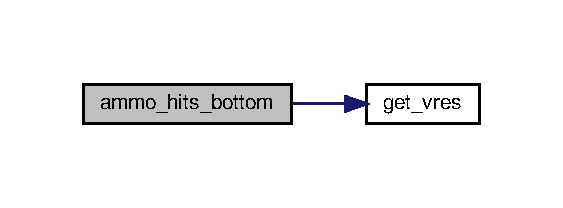
\includegraphics[width=270pt]{group__ammo_gaec2edee56f7204786a3640973e4f8f7f_cgraph}
\end{center}
\end{figure}
\mbox{\Hypertarget{group__ammo_ga23525b3b56d7c2217da8179045d80db6}\label{group__ammo_ga23525b3b56d7c2217da8179045d80db6}} 
\index{ammo@{ammo}!ammo\+\_\+hits\+\_\+left@{ammo\+\_\+hits\+\_\+left}}
\index{ammo\+\_\+hits\+\_\+left@{ammo\+\_\+hits\+\_\+left}!ammo@{ammo}}
\subsubsection{\texorpdfstring{ammo\+\_\+hits\+\_\+left()}{ammo\_hits\_left()}}
{\footnotesize\ttfamily bool ammo\+\_\+hits\+\_\+left (\begin{DoxyParamCaption}\item[{\hyperlink{structammo}{ammo} $\ast$}]{b }\end{DoxyParamCaption})}


\begin{DoxyParams}{Parameters}
{\em b} & A pointer to the ammo we want to check \\
\hline
\end{DoxyParams}
\begin{DoxyReturn}{Returns}
true if the ammo is hitting the left of the screen, otherwise false 
\end{DoxyReturn}
\mbox{\Hypertarget{group__ammo_gabab3a68eb48f6e4f339c648f6cec5522}\label{group__ammo_gabab3a68eb48f6e4f339c648f6cec5522}} 
\index{ammo@{ammo}!ammo\+\_\+hits\+\_\+right@{ammo\+\_\+hits\+\_\+right}}
\index{ammo\+\_\+hits\+\_\+right@{ammo\+\_\+hits\+\_\+right}!ammo@{ammo}}
\subsubsection{\texorpdfstring{ammo\+\_\+hits\+\_\+right()}{ammo\_hits\_right()}}
{\footnotesize\ttfamily bool ammo\+\_\+hits\+\_\+right (\begin{DoxyParamCaption}\item[{\hyperlink{structammo}{ammo} $\ast$}]{b }\end{DoxyParamCaption})}


\begin{DoxyParams}{Parameters}
{\em b} & A pointer to the ammo we want to check \\
\hline
\end{DoxyParams}
\begin{DoxyReturn}{Returns}
true if the ammo is hitting the right of the screen, otherwise false 
\end{DoxyReturn}
Here is the call graph for this function\+:\nopagebreak
\begin{figure}[H]
\begin{center}
\leavevmode
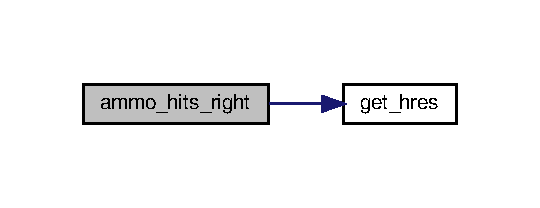
\includegraphics[width=259pt]{group__ammo_gabab3a68eb48f6e4f339c648f6cec5522_cgraph}
\end{center}
\end{figure}
\mbox{\Hypertarget{group__ammo_ga05181ac613d5d6d1d1070031b5461191}\label{group__ammo_ga05181ac613d5d6d1d1070031b5461191}} 
\index{ammo@{ammo}!ammo\+\_\+hits\+\_\+top@{ammo\+\_\+hits\+\_\+top}}
\index{ammo\+\_\+hits\+\_\+top@{ammo\+\_\+hits\+\_\+top}!ammo@{ammo}}
\subsubsection{\texorpdfstring{ammo\+\_\+hits\+\_\+top()}{ammo\_hits\_top()}}
{\footnotesize\ttfamily bool ammo\+\_\+hits\+\_\+top (\begin{DoxyParamCaption}\item[{\hyperlink{structammo}{ammo} $\ast$}]{b }\end{DoxyParamCaption})}


\begin{DoxyParams}{Parameters}
{\em b} & A pointer to the ammo we want to check \\
\hline
\end{DoxyParams}
\begin{DoxyReturn}{Returns}
true if the ammo is hitting the top of the screen, otherwise false 
\end{DoxyReturn}
\mbox{\Hypertarget{group__ammo_ga4d649b8b03319d3a2cdc2f171f9112ea}\label{group__ammo_ga4d649b8b03319d3a2cdc2f171f9112ea}} 
\index{ammo@{ammo}!draw\+\_\+ammo@{draw\+\_\+ammo}}
\index{draw\+\_\+ammo@{draw\+\_\+ammo}!ammo@{ammo}}
\subsubsection{\texorpdfstring{draw\+\_\+ammo()}{draw\_ammo()}}
{\footnotesize\ttfamily void draw\+\_\+ammo (\begin{DoxyParamCaption}\item[{uint8\+\_\+t $\ast$}]{base\+\_\+ptr }\end{DoxyParamCaption})}



Draws the ammo \char`\"{}balls\char`\"{} (that are active) on the given buffer. 


\begin{DoxyParams}{Parameters}
{\em base\+\_\+ptr} & A pointer to a buffer (must be equal in size to the frame buffer) \\
\hline
\end{DoxyParams}
Here is the call graph for this function\+:\nopagebreak
\begin{figure}[H]
\begin{center}
\leavevmode
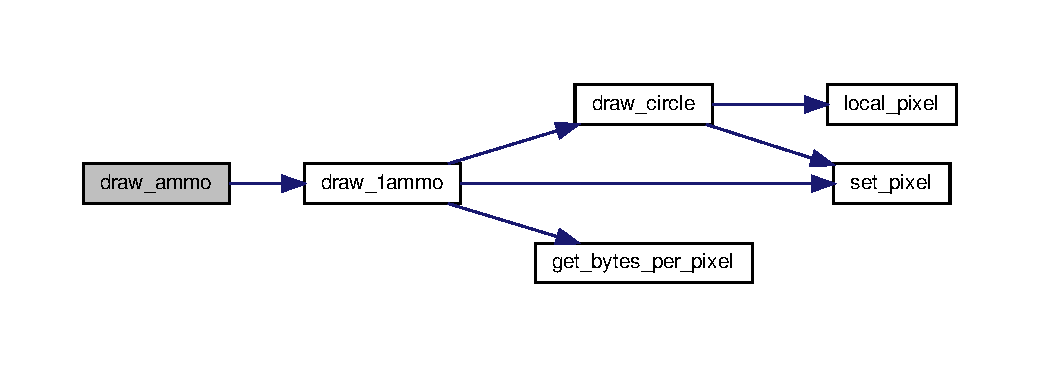
\includegraphics[width=350pt]{group__ammo_ga4d649b8b03319d3a2cdc2f171f9112ea_cgraph}
\end{center}
\end{figure}
\mbox{\Hypertarget{group__ammo_gafd32649160360f67e00c8dc8186edeef}\label{group__ammo_gafd32649160360f67e00c8dc8186edeef}} 
\index{ammo@{ammo}!get\+\_\+ammo@{get\+\_\+ammo}}
\index{get\+\_\+ammo@{get\+\_\+ammo}!ammo@{ammo}}
\subsubsection{\texorpdfstring{get\+\_\+ammo()}{get\_ammo()}}
{\footnotesize\ttfamily \hyperlink{structammo}{ammo}$\ast$ get\+\_\+ammo (\begin{DoxyParamCaption}\item[{uint8\+\_\+t}]{n }\end{DoxyParamCaption})}


\begin{DoxyParams}{Parameters}
{\em n} & either 1, 2 or 3 \\
\hline
\end{DoxyParams}
\begin{DoxyReturn}{Returns}
An ammo pointer 
\end{DoxyReturn}
\mbox{\Hypertarget{group__ammo_gac8e56296d8320fc25379a842c74fd72e}\label{group__ammo_gac8e56296d8320fc25379a842c74fd72e}} 
\index{ammo@{ammo}!spawn\+\_\+ammo@{spawn\+\_\+ammo}}
\index{spawn\+\_\+ammo@{spawn\+\_\+ammo}!ammo@{ammo}}
\subsubsection{\texorpdfstring{spawn\+\_\+ammo()}{spawn\_ammo()}}
{\footnotesize\ttfamily void spawn\+\_\+ammo (\begin{DoxyParamCaption}{ }\end{DoxyParamCaption})}



Spawns an ammo \char`\"{}ball\char`\"{}. 

Here is the call graph for this function\+:\nopagebreak
\begin{figure}[H]
\begin{center}
\leavevmode
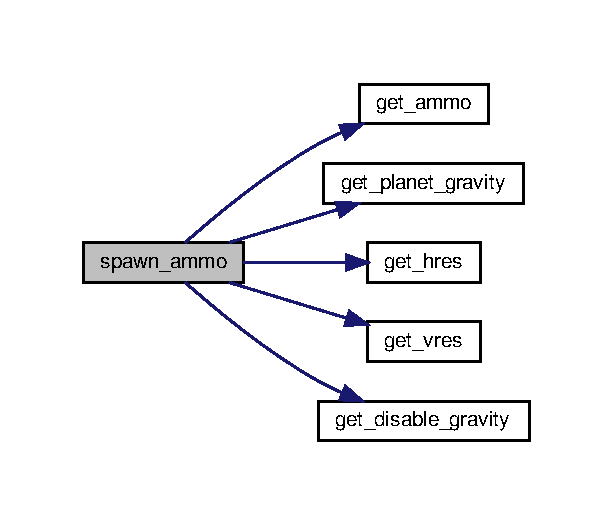
\includegraphics[width=294pt]{group__ammo_gac8e56296d8320fc25379a842c74fd72e_cgraph}
\end{center}
\end{figure}

\hypertarget{group__circle}{}\section{circle}
\label{group__circle}\index{circle@{circle}}


Circle drawing and collision-\/checking functions.  


\subsection*{Functions}
\begin{DoxyCompactItemize}
\item 
bool \hyperlink{group__circle_gaf097cd6cfd9dde8acf534b2c2e1dbabd}{local\+\_\+pixel} (uint16\+\_\+t x\+\_\+pixel, uint16\+\_\+t y\+\_\+pixel, uint16\+\_\+t x1, uint16\+\_\+t y1, uint16\+\_\+t r)
\begin{DoxyCompactList}\small\item\em Checks whether or not a given point is inside a circle. \end{DoxyCompactList}\item 
void \hyperlink{group__circle_gad0932d378de29bbdb27306adf7927591}{draw\+\_\+circle} (uint8\+\_\+t $\ast$base\+\_\+ptr, uint16\+\_\+t x1, uint16\+\_\+t y1, uint16\+\_\+t r, uint32\+\_\+t color)
\begin{DoxyCompactList}\small\item\em Draws a circle on the given buffer with the given center, radius and color. \end{DoxyCompactList}\end{DoxyCompactItemize}


\subsection{Detailed Description}
Circle drawing and collision-\/checking functions. 



\subsection{Function Documentation}
\mbox{\Hypertarget{group__circle_gad0932d378de29bbdb27306adf7927591}\label{group__circle_gad0932d378de29bbdb27306adf7927591}} 
\index{circle@{circle}!draw\+\_\+circle@{draw\+\_\+circle}}
\index{draw\+\_\+circle@{draw\+\_\+circle}!circle@{circle}}
\subsubsection{\texorpdfstring{draw\+\_\+circle()}{draw\_circle()}}
{\footnotesize\ttfamily void draw\+\_\+circle (\begin{DoxyParamCaption}\item[{uint8\+\_\+t $\ast$}]{base\+\_\+ptr,  }\item[{uint16\+\_\+t}]{x1,  }\item[{uint16\+\_\+t}]{y1,  }\item[{uint16\+\_\+t}]{r,  }\item[{uint32\+\_\+t}]{color }\end{DoxyParamCaption})}



Draws a circle on the given buffer with the given center, radius and color. 


\begin{DoxyParams}{Parameters}
{\em base\+\_\+ptr} & A pointer to a buffer (must be equal in size to the frame buffer) \\
\hline
{\em x1} & The x coordinate of the center of the circle \\
\hline
{\em y1} & The y coordinate of the center of the circle \\
\hline
{\em r} & The radius of the circle \\
\hline
{\em color} & The color of the circle \\
\hline
\end{DoxyParams}
Here is the call graph for this function\+:\nopagebreak
\begin{figure}[H]
\begin{center}
\leavevmode
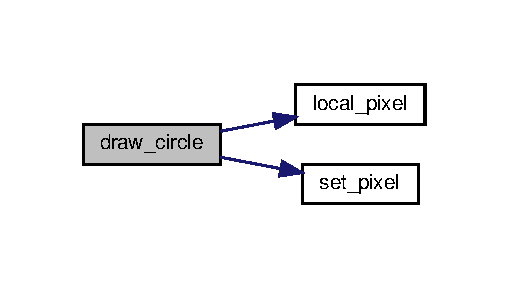
\includegraphics[width=244pt]{group__circle_gad0932d378de29bbdb27306adf7927591_cgraph}
\end{center}
\end{figure}
\mbox{\Hypertarget{group__circle_gaf097cd6cfd9dde8acf534b2c2e1dbabd}\label{group__circle_gaf097cd6cfd9dde8acf534b2c2e1dbabd}} 
\index{circle@{circle}!local\+\_\+pixel@{local\+\_\+pixel}}
\index{local\+\_\+pixel@{local\+\_\+pixel}!circle@{circle}}
\subsubsection{\texorpdfstring{local\+\_\+pixel()}{local\_pixel()}}
{\footnotesize\ttfamily bool local\+\_\+pixel (\begin{DoxyParamCaption}\item[{uint16\+\_\+t}]{x\+\_\+pixel,  }\item[{uint16\+\_\+t}]{y\+\_\+pixel,  }\item[{uint16\+\_\+t}]{x1,  }\item[{uint16\+\_\+t}]{y1,  }\item[{uint16\+\_\+t}]{r }\end{DoxyParamCaption})}



Checks whether or not a given point is inside a circle. 


\begin{DoxyParams}{Parameters}
{\em x\+\_\+pixel} & The x coordinate of the point to be checked \\
\hline
{\em y\+\_\+pixel} & The y coordinate of the point to be checked \\
\hline
{\em x1} & The x coordinate of the center of the circle \\
\hline
{\em y1} & The y coordinate of the center of the circle \\
\hline
{\em r} & The radius of the circle\\
\hline
\end{DoxyParams}
\begin{DoxyReturn}{Returns}
true if the pixel is inside of the circle, otherwise false 
\end{DoxyReturn}

\hypertarget{group__core__game__loop}{}\section{core\+\_\+game\+\_\+loop}
\label{group__core__game__loop}\index{core\+\_\+game\+\_\+loop@{core\+\_\+game\+\_\+loop}}


Houses all the game logic, physics, collisions, rendering and interrupt-\/handling functions.  


\subsection*{Functions}
\begin{DoxyCompactItemize}
\item 
void \hyperlink{group__core__game__loop_ga46e6c6f53965490e91d8629d528ec797}{gravity\+\_\+step} ()
\begin{DoxyCompactList}\small\item\em The high-\/level physics function. \end{DoxyCompactList}\item 
void \hyperlink{group__core__game__loop_ga549153b90f3cb4e43291079eb5d893bf}{explode\+\_\+player} (uint8\+\_\+t \hyperlink{structplayer}{player})
\begin{DoxyCompactList}\small\item\em Explodes one of the players Rather unsurprisingly, calls to this function usually imply the end of the game. \end{DoxyCompactList}\item 
void \hyperlink{group__core__game__loop_gadffa4aa993db001bdee35fbce31dc00b}{player\+\_\+deal\+\_\+damage} (uint8\+\_\+t \hyperlink{structplayer}{player}, uint16\+\_\+t damage)
\begin{DoxyCompactList}\small\item\em Deals damage one of the players. If the player doesn\textquotesingle{}t have enough HP to take the hit, \hyperlink{group__core__game__loop_ga549153b90f3cb4e43291079eb5d893bf}{explode\+\_\+player(uint8\+\_\+t player)} is called and the game ends. \end{DoxyCompactList}\item 
void \hyperlink{group__core__game__loop_ga7ffe05c55466ca7e6c94b73b63c22927}{player\+\_\+shoot} (\hyperlink{structplayer}{player} $\ast$p)
\begin{DoxyCompactList}\small\item\em Spawns a projectile in front of p, with a given velocity. \end{DoxyCompactList}\item 
void \hyperlink{group__core__game__loop_ga79bddd8b336f6be116bfa658dd949e2e}{shooting} ()
\begin{DoxyCompactList}\small\item\em The high-\/level shooting function. \end{DoxyCompactList}\item 
void \hyperlink{group__core__game__loop_ga53d6cc2e012c3f117efb3cd959af4af4}{collision} ()
\begin{DoxyCompactList}\small\item\em The high-\/level collision-\/checking function. \end{DoxyCompactList}\item 
void \hyperlink{group__core__game__loop_ga9f1bba2db0aa13b5749945e9679a28bc}{draw\+\_\+life\+\_\+bars} (uint8\+\_\+t $\ast$base\+\_\+ptr)
\begin{DoxyCompactList}\small\item\em Draws the players\textquotesingle{} life bars. \end{DoxyCompactList}\item 
void \hyperlink{group__core__game__loop_ga33240cb1f9e3570ad230d7e081888dd6}{draw\+\_\+transparent\+\_\+image} (uint8\+\_\+t $\ast$base\+\_\+ptr, uint16\+\_\+t x, uint16\+\_\+t y, xpm\+\_\+image\+\_\+t img, bool invert)
\begin{DoxyCompactList}\small\item\em Pretty much the same as \hyperlink{group__video__card_gacd25f5efb8e27da60488e6b317be5e12}{set\+\_\+xpm\+\_\+image(uint8\+\_\+t $\ast$base\+\_\+ptr, uint16\+\_\+t x, uint16\+\_\+t y, xpm\+\_\+image\+\_\+t img)}, with the notable exception that white pixels do not get drawn. \end{DoxyCompactList}\item 
void \hyperlink{group__core__game__loop_gade0334b547fb581566867d040aa7608a}{draw\+\_\+message} (uint8\+\_\+t $\ast$base\+\_\+ptr)
\begin{DoxyCompactList}\small\item\em If the game ended, displays a message on the top of the screen. \end{DoxyCompactList}\item 
void \hyperlink{group__core__game__loop_ga40e143893b9f0cd6ae25ab8e3017b5b2}{draw\+\_\+ammo\+\_\+numbers} (uint8\+\_\+t $\ast$base\+\_\+ptr)
\begin{DoxyCompactList}\small\item\em Draws the ammunition numbers, letting them know how many bullets they have. \end{DoxyCompactList}\item 
void \hyperlink{group__core__game__loop_ga56c5cf8a568cff737ff95520cbe6b405}{draw} ()
\begin{DoxyCompactList}\small\item\em The high-\/level frame-\/rendering function. \end{DoxyCompactList}\item 
void \hyperlink{group__core__game__loop_ga46fea93bf5d63e93090fbb95b742b881}{game\+\_\+loop} ()
\begin{DoxyCompactList}\small\item\em The high-\/level game loop function. \end{DoxyCompactList}\item 
void \hyperlink{group__core__game__loop_ga3675a504daf73491a060c7462420df07}{draw\+\_\+sun} (uint8\+\_\+t $\ast$base\+\_\+ptr, uint16\+\_\+t x, uint16\+\_\+t y, xpm\+\_\+image\+\_\+t img)
\begin{DoxyCompactList}\small\item\em Pretty much the same as \hyperlink{group__video__card_gacd25f5efb8e27da60488e6b317be5e12}{set\+\_\+xpm\+\_\+image(uint8\+\_\+t $\ast$base\+\_\+ptr, uint16\+\_\+t x, uint16\+\_\+t y, xpm\+\_\+image\+\_\+t img)}, with the notable exception that only pixels from a given distance from the center of the screen get drawn. \end{DoxyCompactList}\item 
void \hyperlink{group__core__game__loop_gac82e7d55ed069f5d0c396c20b97337e9}{load\+\_\+xpms} ()
\begin{DoxyCompactList}\small\item\em Loads the X\+P\+Ms, if they have not been already loaded. \end{DoxyCompactList}\item 
void \hyperlink{group__core__game__loop_gaa06ba1be9bd4796cb317a83db95966f2}{core\+\_\+game\+\_\+loop} ()
\begin{DoxyCompactList}\small\item\em The highest-\/level function of this module. \end{DoxyCompactList}\end{DoxyCompactItemize}


\subsection{Detailed Description}
Houses all the game logic, physics, collisions, rendering and interrupt-\/handling functions. 



\subsection{Function Documentation}
\mbox{\Hypertarget{group__core__game__loop_ga53d6cc2e012c3f117efb3cd959af4af4}\label{group__core__game__loop_ga53d6cc2e012c3f117efb3cd959af4af4}} 
\index{core\+\_\+game\+\_\+loop@{core\+\_\+game\+\_\+loop}!collision@{collision}}
\index{collision@{collision}!core\+\_\+game\+\_\+loop@{core\+\_\+game\+\_\+loop}}
\subsubsection{\texorpdfstring{collision()}{collision()}}
{\footnotesize\ttfamily void collision (\begin{DoxyParamCaption}{ }\end{DoxyParamCaption})}



The high-\/level collision-\/checking function. 

It performs collision checks and processing for each player, projectile and ammo Here is the call graph for this function\+:\nopagebreak
\begin{figure}[H]
\begin{center}
\leavevmode
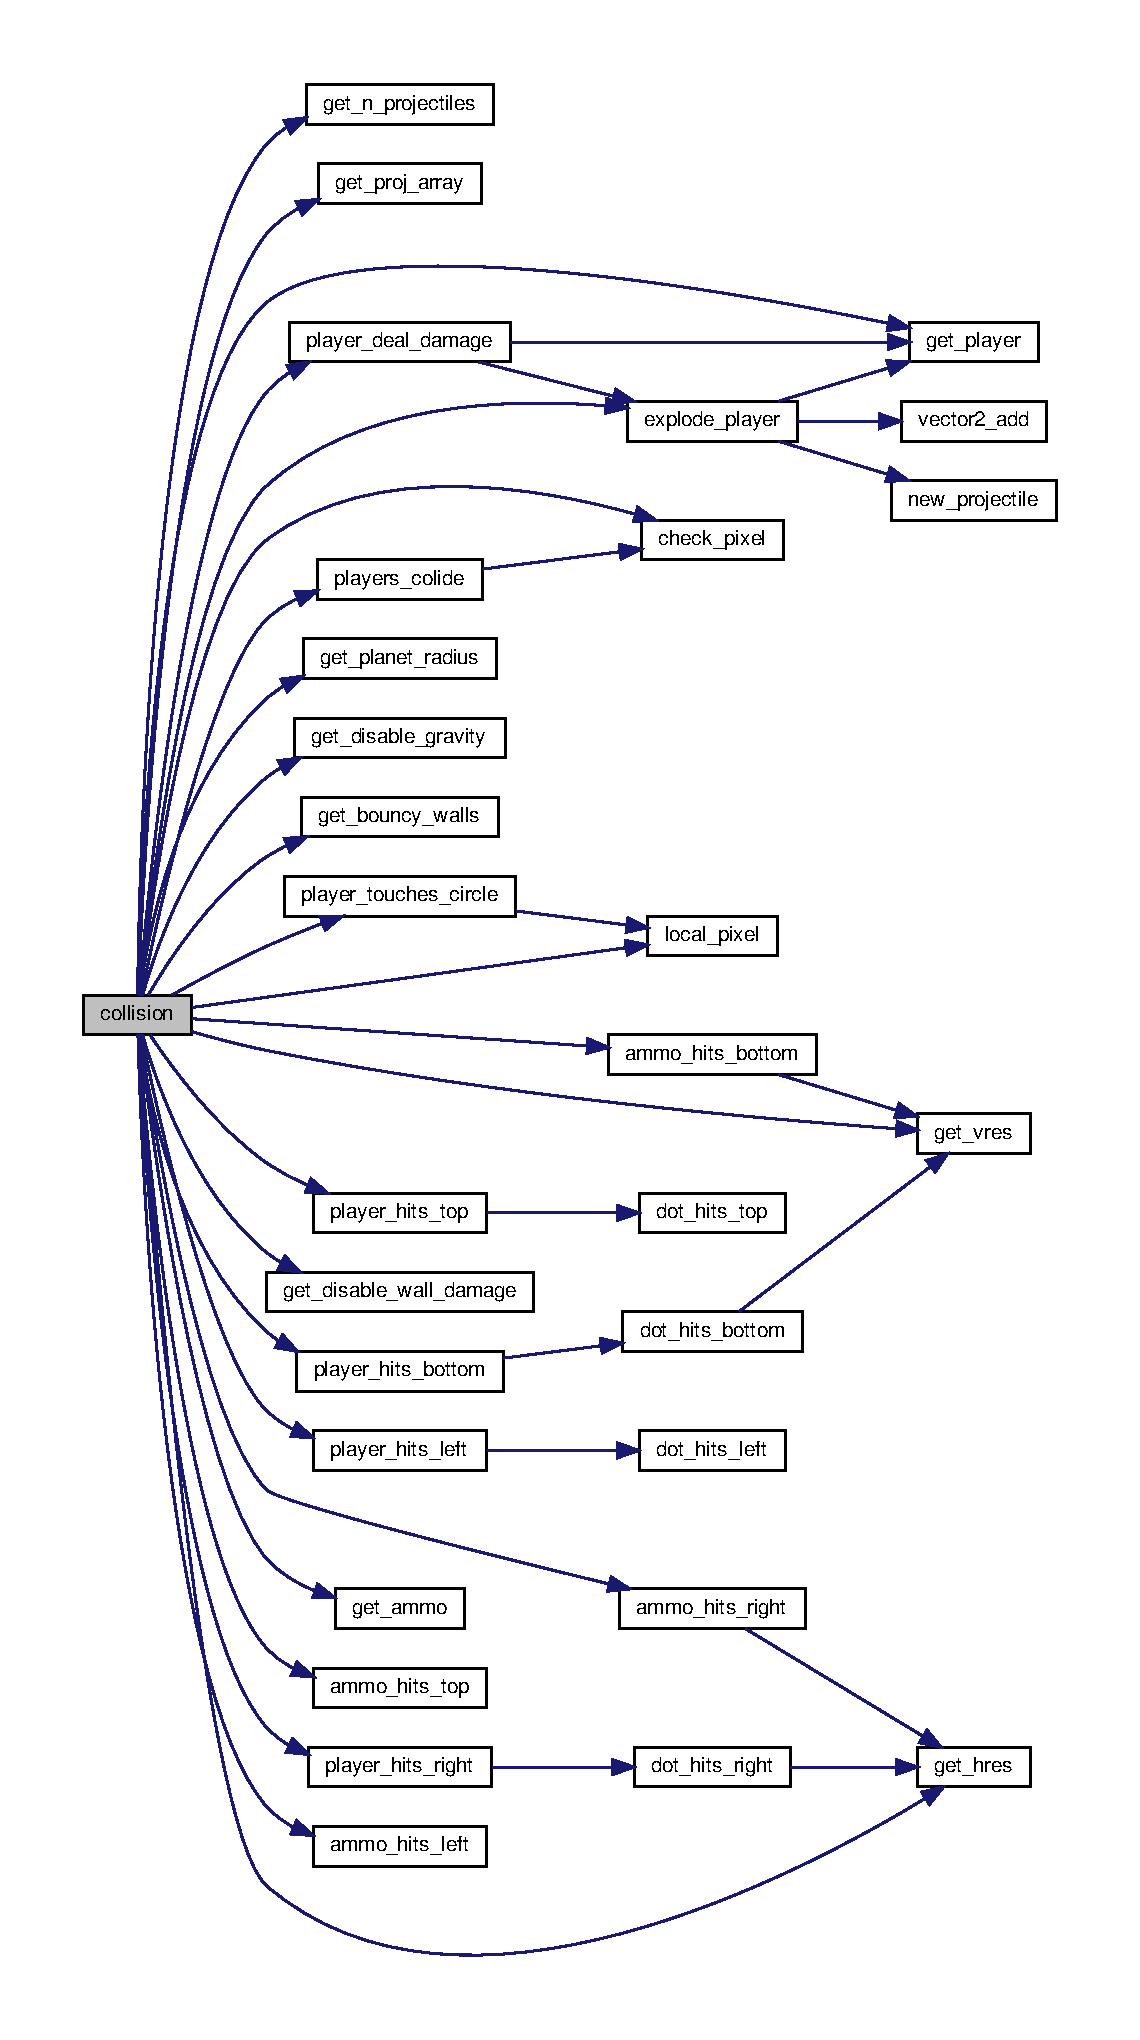
\includegraphics[height=550pt]{group__core__game__loop_ga53d6cc2e012c3f117efb3cd959af4af4_cgraph}
\end{center}
\end{figure}
\mbox{\Hypertarget{group__core__game__loop_gaa06ba1be9bd4796cb317a83db95966f2}\label{group__core__game__loop_gaa06ba1be9bd4796cb317a83db95966f2}} 
\index{core\+\_\+game\+\_\+loop@{core\+\_\+game\+\_\+loop}!core\+\_\+game\+\_\+loop@{core\+\_\+game\+\_\+loop}}
\index{core\+\_\+game\+\_\+loop@{core\+\_\+game\+\_\+loop}!core\+\_\+game\+\_\+loop@{core\+\_\+game\+\_\+loop}}
\subsubsection{\texorpdfstring{core\+\_\+game\+\_\+loop()}{core\_game\_loop()}}
{\footnotesize\ttfamily void core\+\_\+game\+\_\+loop (\begin{DoxyParamCaption}{ }\end{DoxyParamCaption})}



The highest-\/level function of this module. 

It deals not only with interruption subscribing/handling/unsubscribing but also with game related initialization Here is the call graph for this function\+:\nopagebreak
\begin{figure}[H]
\begin{center}
\leavevmode
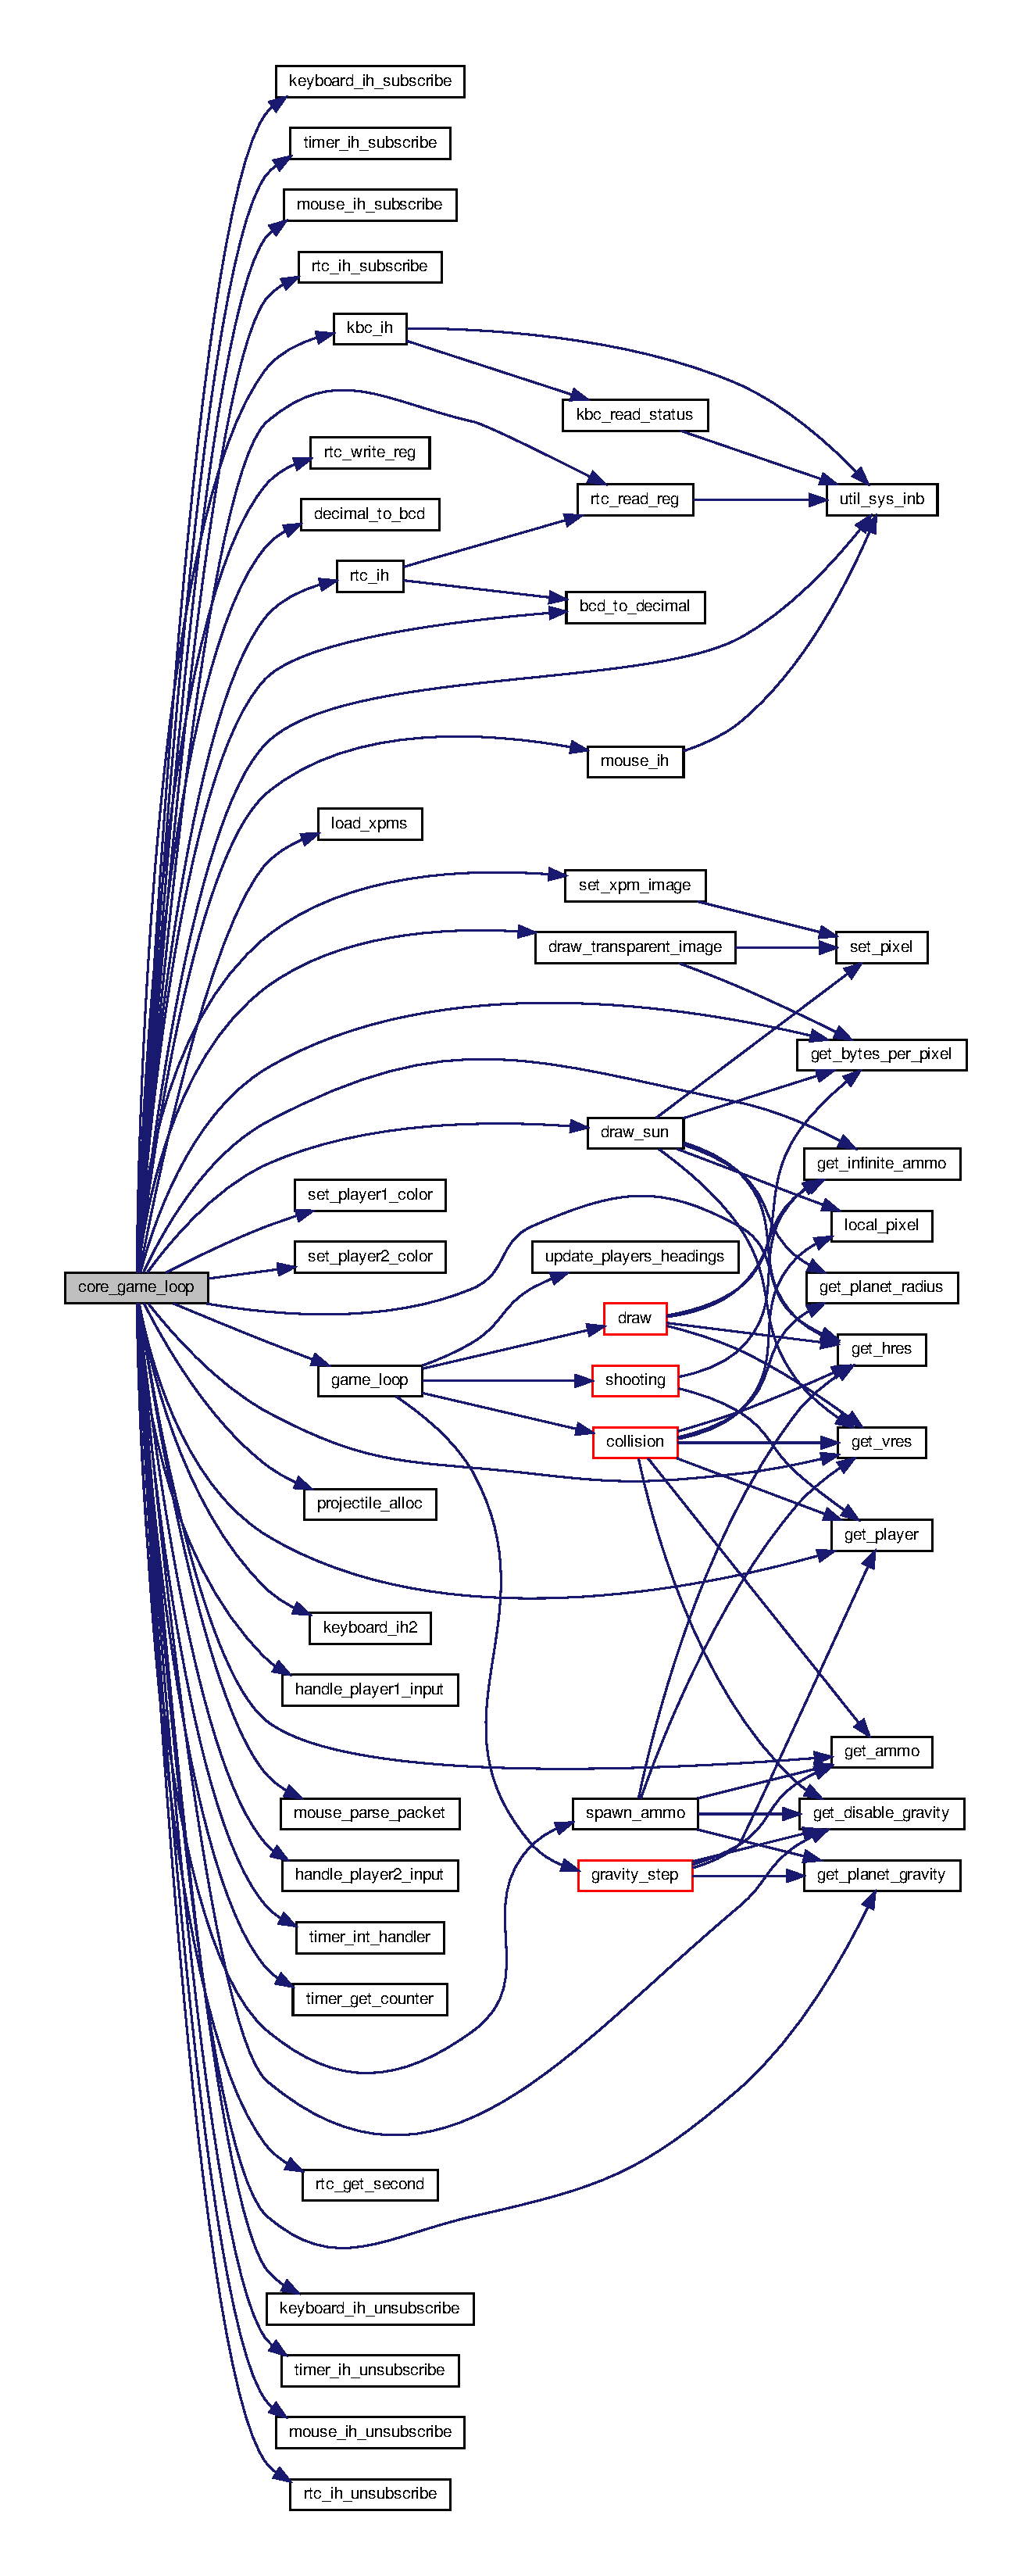
\includegraphics[height=550pt]{group__core__game__loop_gaa06ba1be9bd4796cb317a83db95966f2_cgraph}
\end{center}
\end{figure}
\mbox{\Hypertarget{group__core__game__loop_ga56c5cf8a568cff737ff95520cbe6b405}\label{group__core__game__loop_ga56c5cf8a568cff737ff95520cbe6b405}} 
\index{core\+\_\+game\+\_\+loop@{core\+\_\+game\+\_\+loop}!draw@{draw}}
\index{draw@{draw}!core\+\_\+game\+\_\+loop@{core\+\_\+game\+\_\+loop}}
\subsubsection{\texorpdfstring{draw()}{draw()}}
{\footnotesize\ttfamily void draw (\begin{DoxyParamCaption}{ }\end{DoxyParamCaption})}



The high-\/level frame-\/rendering function. 

It copies a background buffer (a buffer with background static stuff) to the double buffer, draws all the game-\/related objects and UI, and finishes off by copying the double buffer to the frame buffer. Here is the call graph for this function\+:\nopagebreak
\begin{figure}[H]
\begin{center}
\leavevmode
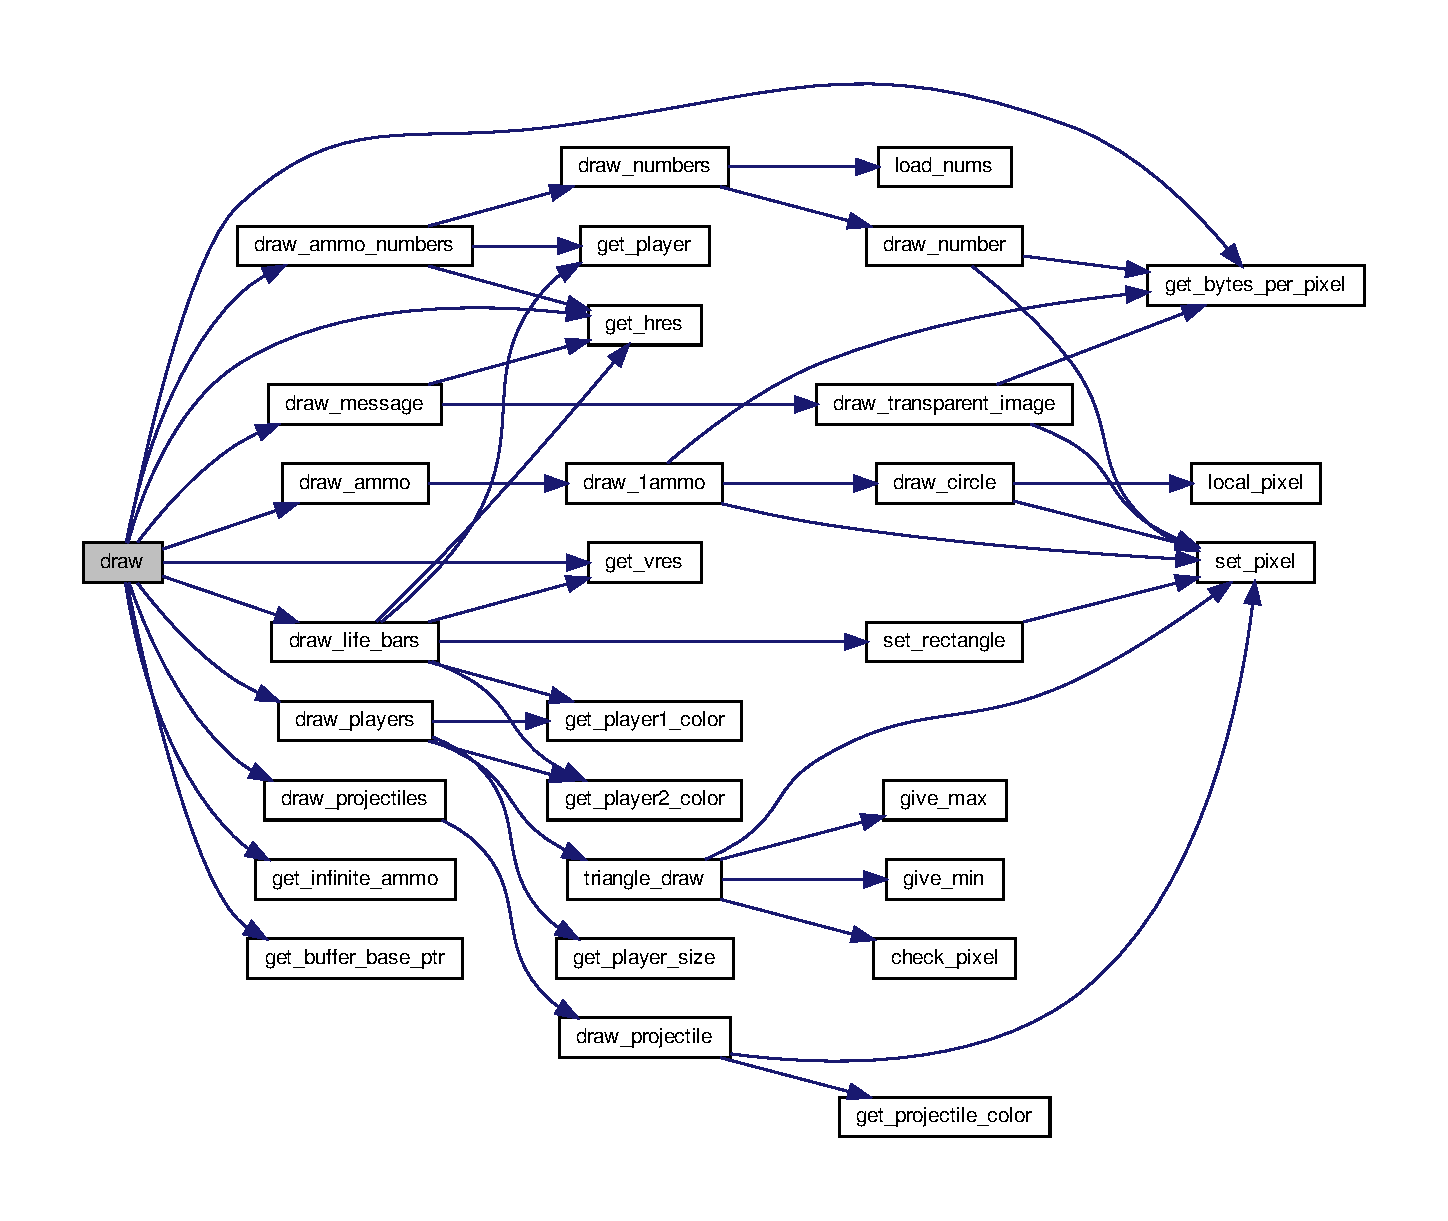
\includegraphics[width=350pt]{group__core__game__loop_ga56c5cf8a568cff737ff95520cbe6b405_cgraph}
\end{center}
\end{figure}
\mbox{\Hypertarget{group__core__game__loop_ga40e143893b9f0cd6ae25ab8e3017b5b2}\label{group__core__game__loop_ga40e143893b9f0cd6ae25ab8e3017b5b2}} 
\index{core\+\_\+game\+\_\+loop@{core\+\_\+game\+\_\+loop}!draw\+\_\+ammo\+\_\+numbers@{draw\+\_\+ammo\+\_\+numbers}}
\index{draw\+\_\+ammo\+\_\+numbers@{draw\+\_\+ammo\+\_\+numbers}!core\+\_\+game\+\_\+loop@{core\+\_\+game\+\_\+loop}}
\subsubsection{\texorpdfstring{draw\+\_\+ammo\+\_\+numbers()}{draw\_ammo\_numbers()}}
{\footnotesize\ttfamily void draw\+\_\+ammo\+\_\+numbers (\begin{DoxyParamCaption}\item[{uint8\+\_\+t $\ast$}]{base\+\_\+ptr }\end{DoxyParamCaption})}



Draws the ammunition numbers, letting them know how many bullets they have. 


\begin{DoxyParams}{Parameters}
{\em base\+\_\+ptr} & A pointer to a buffer (must be equal in size to the frame buffer) \\
\hline
\end{DoxyParams}
Here is the call graph for this function\+:\nopagebreak
\begin{figure}[H]
\begin{center}
\leavevmode
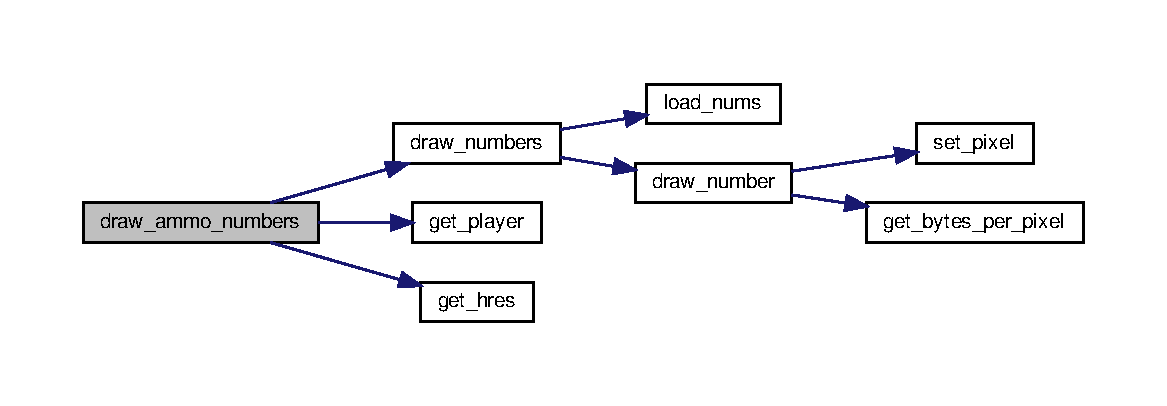
\includegraphics[width=350pt]{group__core__game__loop_ga40e143893b9f0cd6ae25ab8e3017b5b2_cgraph}
\end{center}
\end{figure}
\mbox{\Hypertarget{group__core__game__loop_ga9f1bba2db0aa13b5749945e9679a28bc}\label{group__core__game__loop_ga9f1bba2db0aa13b5749945e9679a28bc}} 
\index{core\+\_\+game\+\_\+loop@{core\+\_\+game\+\_\+loop}!draw\+\_\+life\+\_\+bars@{draw\+\_\+life\+\_\+bars}}
\index{draw\+\_\+life\+\_\+bars@{draw\+\_\+life\+\_\+bars}!core\+\_\+game\+\_\+loop@{core\+\_\+game\+\_\+loop}}
\subsubsection{\texorpdfstring{draw\+\_\+life\+\_\+bars()}{draw\_life\_bars()}}
{\footnotesize\ttfamily void draw\+\_\+life\+\_\+bars (\begin{DoxyParamCaption}\item[{uint8\+\_\+t $\ast$}]{base\+\_\+ptr }\end{DoxyParamCaption})}



Draws the players\textquotesingle{} life bars. 


\begin{DoxyParams}{Parameters}
{\em base\+\_\+ptr} & A pointer to a buffer (must be equal in size to the frame buffer) \\
\hline
\end{DoxyParams}
Here is the call graph for this function\+:\nopagebreak
\begin{figure}[H]
\begin{center}
\leavevmode
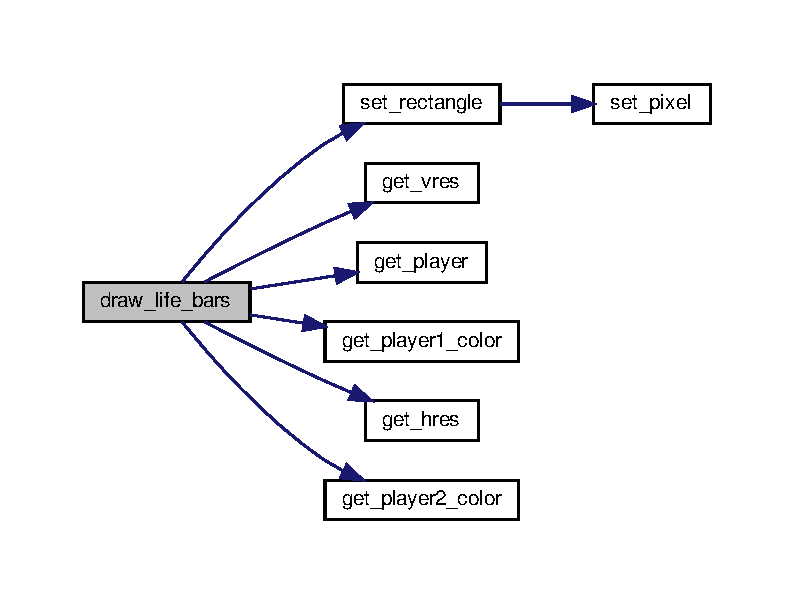
\includegraphics[width=350pt]{group__core__game__loop_ga9f1bba2db0aa13b5749945e9679a28bc_cgraph}
\end{center}
\end{figure}
\mbox{\Hypertarget{group__core__game__loop_gade0334b547fb581566867d040aa7608a}\label{group__core__game__loop_gade0334b547fb581566867d040aa7608a}} 
\index{core\+\_\+game\+\_\+loop@{core\+\_\+game\+\_\+loop}!draw\+\_\+message@{draw\+\_\+message}}
\index{draw\+\_\+message@{draw\+\_\+message}!core\+\_\+game\+\_\+loop@{core\+\_\+game\+\_\+loop}}
\subsubsection{\texorpdfstring{draw\+\_\+message()}{draw\_message()}}
{\footnotesize\ttfamily void draw\+\_\+message (\begin{DoxyParamCaption}\item[{uint8\+\_\+t $\ast$}]{base\+\_\+ptr }\end{DoxyParamCaption})}



If the game ended, displays a message on the top of the screen. 


\begin{DoxyParams}{Parameters}
{\em base\+\_\+ptr} & A pointer to a buffer (must be equal in size to the frame buffer) \\
\hline
\end{DoxyParams}
Here is the call graph for this function\+:\nopagebreak
\begin{figure}[H]
\begin{center}
\leavevmode
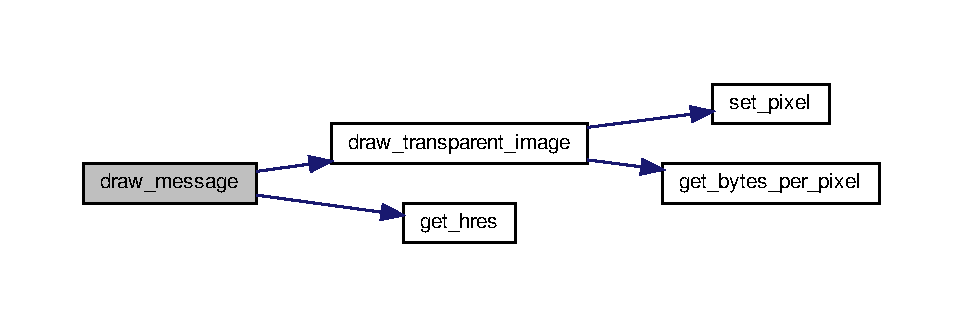
\includegraphics[width=350pt]{group__core__game__loop_gade0334b547fb581566867d040aa7608a_cgraph}
\end{center}
\end{figure}
\mbox{\Hypertarget{group__core__game__loop_ga3675a504daf73491a060c7462420df07}\label{group__core__game__loop_ga3675a504daf73491a060c7462420df07}} 
\index{core\+\_\+game\+\_\+loop@{core\+\_\+game\+\_\+loop}!draw\+\_\+sun@{draw\+\_\+sun}}
\index{draw\+\_\+sun@{draw\+\_\+sun}!core\+\_\+game\+\_\+loop@{core\+\_\+game\+\_\+loop}}
\subsubsection{\texorpdfstring{draw\+\_\+sun()}{draw\_sun()}}
{\footnotesize\ttfamily void draw\+\_\+sun (\begin{DoxyParamCaption}\item[{uint8\+\_\+t $\ast$}]{base\+\_\+ptr,  }\item[{uint16\+\_\+t}]{x,  }\item[{uint16\+\_\+t}]{y,  }\item[{xpm\+\_\+image\+\_\+t}]{img }\end{DoxyParamCaption})}



Pretty much the same as \hyperlink{group__video__card_gacd25f5efb8e27da60488e6b317be5e12}{set\+\_\+xpm\+\_\+image(uint8\+\_\+t $\ast$base\+\_\+ptr, uint16\+\_\+t x, uint16\+\_\+t y, xpm\+\_\+image\+\_\+t img)}, with the notable exception that only pixels from a given distance from the center of the screen get drawn. 


\begin{DoxyParams}{Parameters}
{\em base\+\_\+ptr} & A pointer to a buffer (must be equal in size to the frame buffer) \\
\hline
{\em x} & The x coordinate of the top left corner of the xpm image (counting downwards from the top) \\
\hline
{\em y} & The y coordinate of the top left corner of the xpm image (counting rightwards from the left) \\
\hline
{\em img} & The xpm image (see \href{https://web.fe.up.pt/~pfs/aulas/lcom2019/labs/lab5/src/doc/structxpm__image__t.html}{\tt this}) \\
\hline
\end{DoxyParams}
Here is the call graph for this function\+:\nopagebreak
\begin{figure}[H]
\begin{center}
\leavevmode
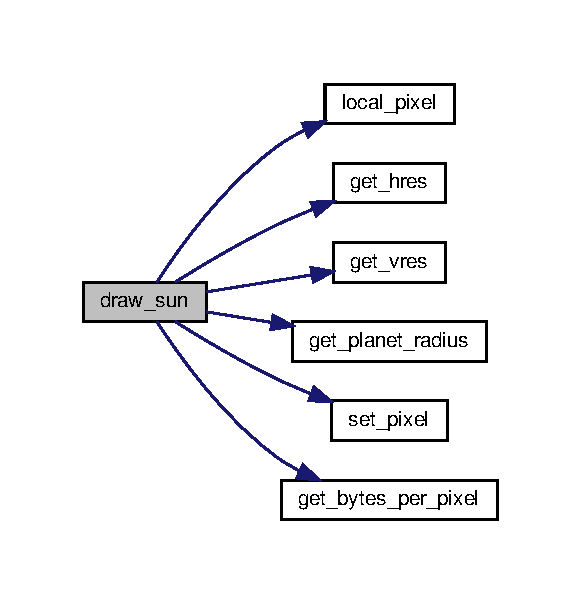
\includegraphics[width=279pt]{group__core__game__loop_ga3675a504daf73491a060c7462420df07_cgraph}
\end{center}
\end{figure}
\mbox{\Hypertarget{group__core__game__loop_ga33240cb1f9e3570ad230d7e081888dd6}\label{group__core__game__loop_ga33240cb1f9e3570ad230d7e081888dd6}} 
\index{core\+\_\+game\+\_\+loop@{core\+\_\+game\+\_\+loop}!draw\+\_\+transparent\+\_\+image@{draw\+\_\+transparent\+\_\+image}}
\index{draw\+\_\+transparent\+\_\+image@{draw\+\_\+transparent\+\_\+image}!core\+\_\+game\+\_\+loop@{core\+\_\+game\+\_\+loop}}
\subsubsection{\texorpdfstring{draw\+\_\+transparent\+\_\+image()}{draw\_transparent\_image()}}
{\footnotesize\ttfamily void draw\+\_\+transparent\+\_\+image (\begin{DoxyParamCaption}\item[{uint8\+\_\+t $\ast$}]{base\+\_\+ptr,  }\item[{uint16\+\_\+t}]{x,  }\item[{uint16\+\_\+t}]{y,  }\item[{xpm\+\_\+image\+\_\+t}]{img,  }\item[{bool}]{invert }\end{DoxyParamCaption})}



Pretty much the same as \hyperlink{group__video__card_gacd25f5efb8e27da60488e6b317be5e12}{set\+\_\+xpm\+\_\+image(uint8\+\_\+t $\ast$base\+\_\+ptr, uint16\+\_\+t x, uint16\+\_\+t y, xpm\+\_\+image\+\_\+t img)}, with the notable exception that white pixels do not get drawn. 


\begin{DoxyParams}{Parameters}
{\em base\+\_\+ptr} & A pointer to a buffer (must be equal in size to the frame buffer) \\
\hline
{\em x} & The x coordinate of the top left corner of the xpm image (counting downwards from the top) \\
\hline
{\em y} & The y coordinate of the top left corner of the xpm image (counting rightwards from the left) \\
\hline
{\em img} & The xpm image (see \href{https://web.fe.up.pt/~pfs/aulas/lcom2019/labs/lab5/src/doc/structxpm__image__t.html}{\tt this}) \\
\hline
{\em invert} & Whether or not the image pixels should be inverted while drawn (white becomes black, etc) \\
\hline
\end{DoxyParams}
Here is the call graph for this function\+:\nopagebreak
\begin{figure}[H]
\begin{center}
\leavevmode
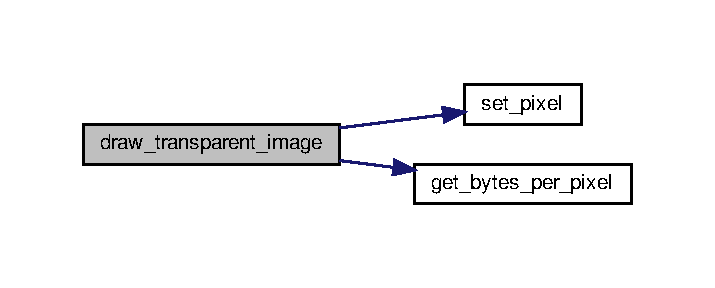
\includegraphics[width=343pt]{group__core__game__loop_ga33240cb1f9e3570ad230d7e081888dd6_cgraph}
\end{center}
\end{figure}
\mbox{\Hypertarget{group__core__game__loop_ga549153b90f3cb4e43291079eb5d893bf}\label{group__core__game__loop_ga549153b90f3cb4e43291079eb5d893bf}} 
\index{core\+\_\+game\+\_\+loop@{core\+\_\+game\+\_\+loop}!explode\+\_\+player@{explode\+\_\+player}}
\index{explode\+\_\+player@{explode\+\_\+player}!core\+\_\+game\+\_\+loop@{core\+\_\+game\+\_\+loop}}
\subsubsection{\texorpdfstring{explode\+\_\+player()}{explode\_player()}}
{\footnotesize\ttfamily void explode\+\_\+player (\begin{DoxyParamCaption}\item[{uint8\+\_\+t}]{player }\end{DoxyParamCaption})}



Explodes one of the players Rather unsurprisingly, calls to this function usually imply the end of the game. 


\begin{DoxyParams}{Parameters}
{\em player} & The number of the player about to be exploded \\
\hline
\end{DoxyParams}
Here is the call graph for this function\+:\nopagebreak
\begin{figure}[H]
\begin{center}
\leavevmode
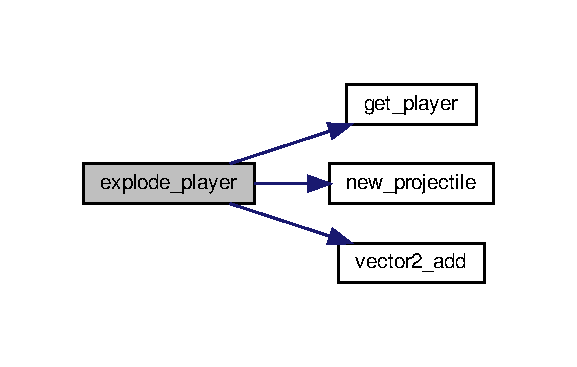
\includegraphics[width=277pt]{group__core__game__loop_ga549153b90f3cb4e43291079eb5d893bf_cgraph}
\end{center}
\end{figure}
\mbox{\Hypertarget{group__core__game__loop_ga46fea93bf5d63e93090fbb95b742b881}\label{group__core__game__loop_ga46fea93bf5d63e93090fbb95b742b881}} 
\index{core\+\_\+game\+\_\+loop@{core\+\_\+game\+\_\+loop}!game\+\_\+loop@{game\+\_\+loop}}
\index{game\+\_\+loop@{game\+\_\+loop}!core\+\_\+game\+\_\+loop@{core\+\_\+game\+\_\+loop}}
\subsubsection{\texorpdfstring{game\+\_\+loop()}{game\_loop()}}
{\footnotesize\ttfamily void game\+\_\+loop (\begin{DoxyParamCaption}{ }\end{DoxyParamCaption})}



The high-\/level game loop function. 

Gets called every frame Here is the call graph for this function\+:\nopagebreak
\begin{figure}[H]
\begin{center}
\leavevmode
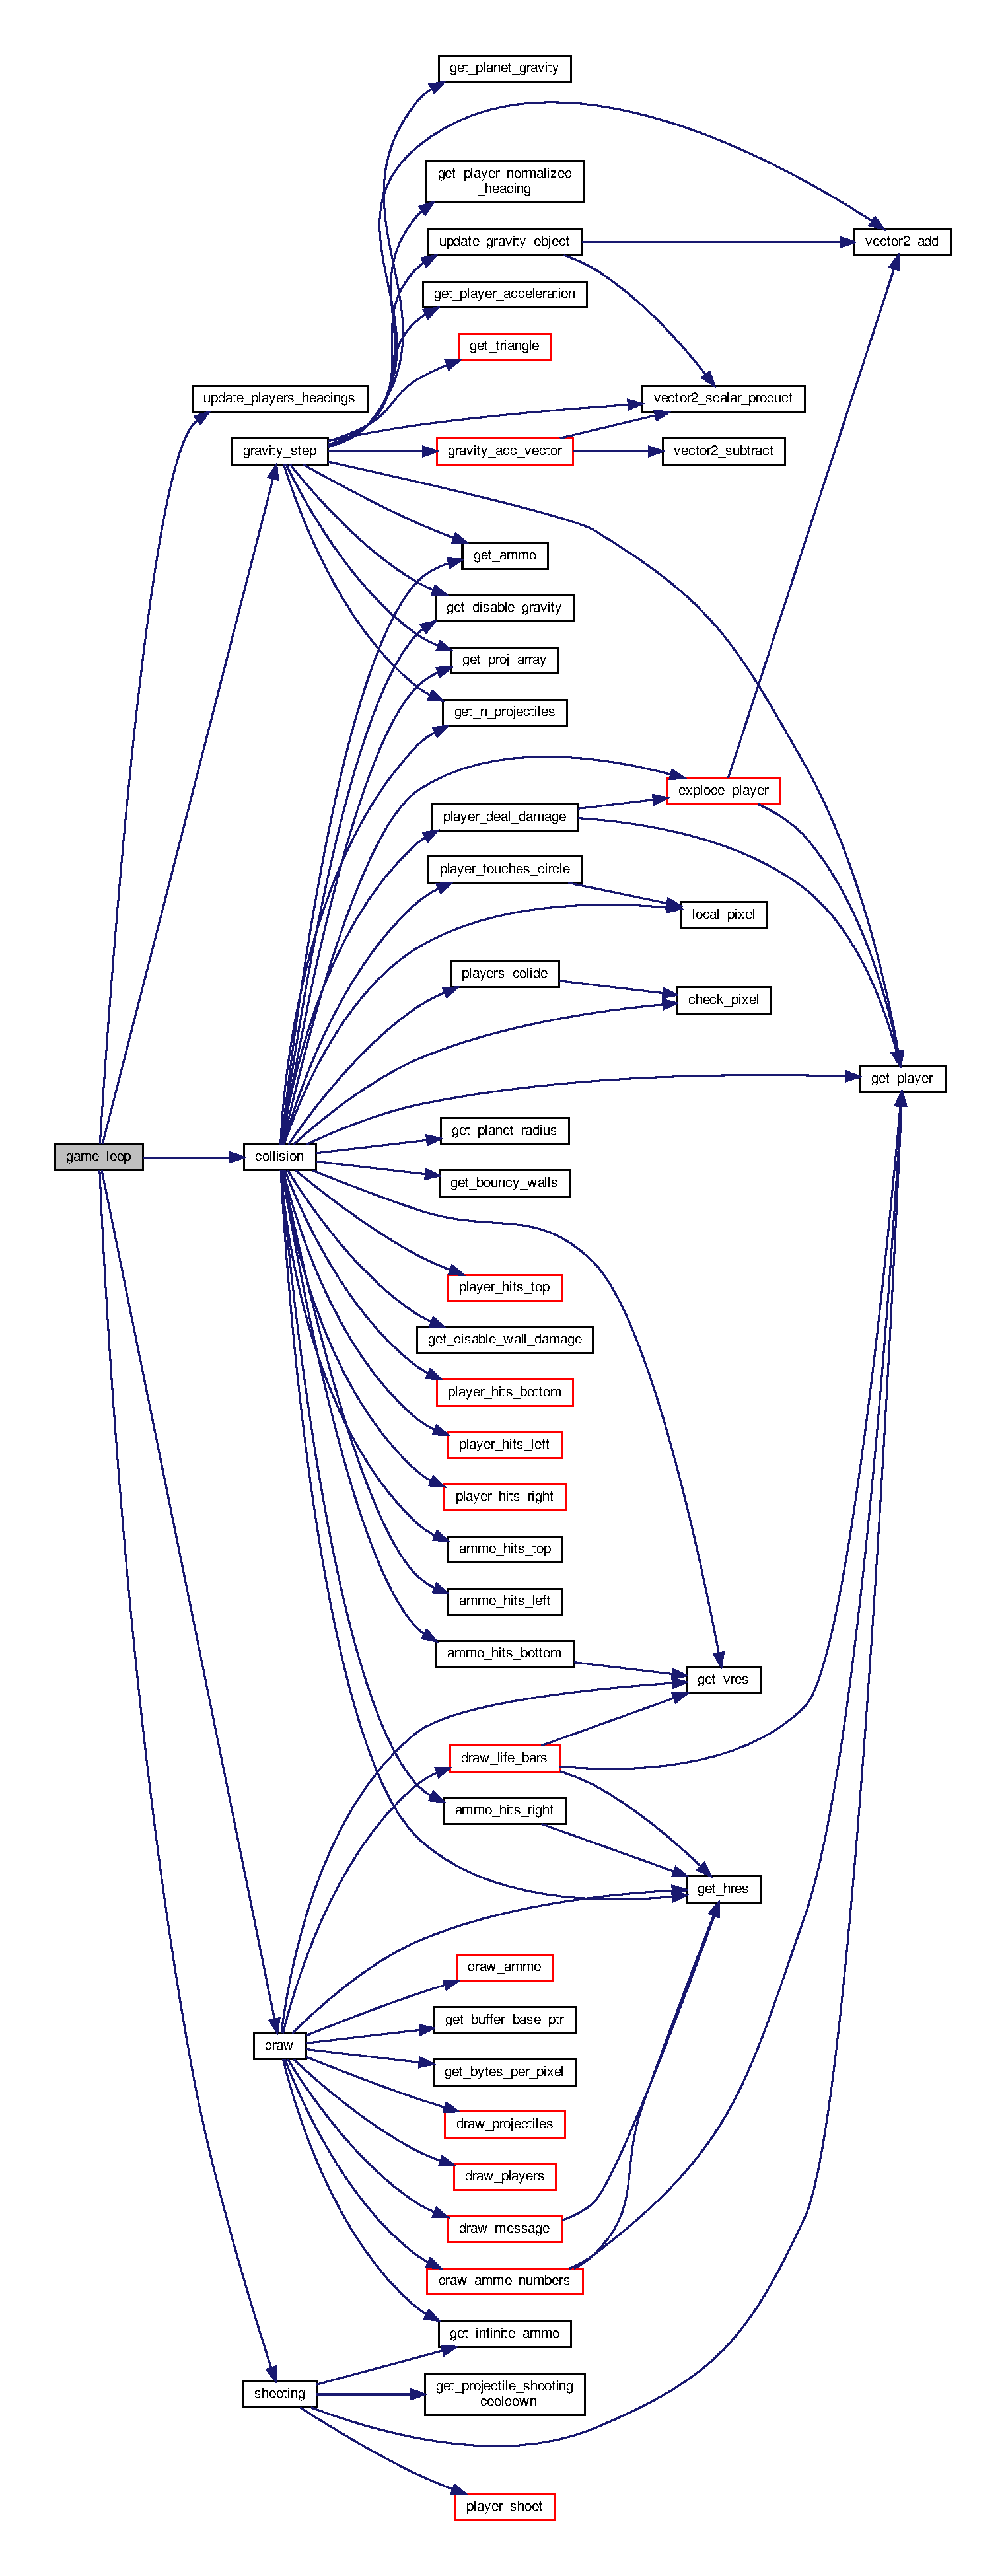
\includegraphics[height=550pt]{group__core__game__loop_ga46fea93bf5d63e93090fbb95b742b881_cgraph}
\end{center}
\end{figure}
\mbox{\Hypertarget{group__core__game__loop_ga46e6c6f53965490e91d8629d528ec797}\label{group__core__game__loop_ga46e6c6f53965490e91d8629d528ec797}} 
\index{core\+\_\+game\+\_\+loop@{core\+\_\+game\+\_\+loop}!gravity\+\_\+step@{gravity\+\_\+step}}
\index{gravity\+\_\+step@{gravity\+\_\+step}!core\+\_\+game\+\_\+loop@{core\+\_\+game\+\_\+loop}}
\subsubsection{\texorpdfstring{gravity\+\_\+step()}{gravity\_step()}}
{\footnotesize\ttfamily void gravity\+\_\+step (\begin{DoxyParamCaption}{ }\end{DoxyParamCaption})}



The high-\/level physics function. 

It updates all of the game objects\textquotesingle{} position for the next frame (players, projectiles and ammo). One can this of this function as a single step of the physics simulation. Here is the call graph for this function\+:\nopagebreak
\begin{figure}[H]
\begin{center}
\leavevmode
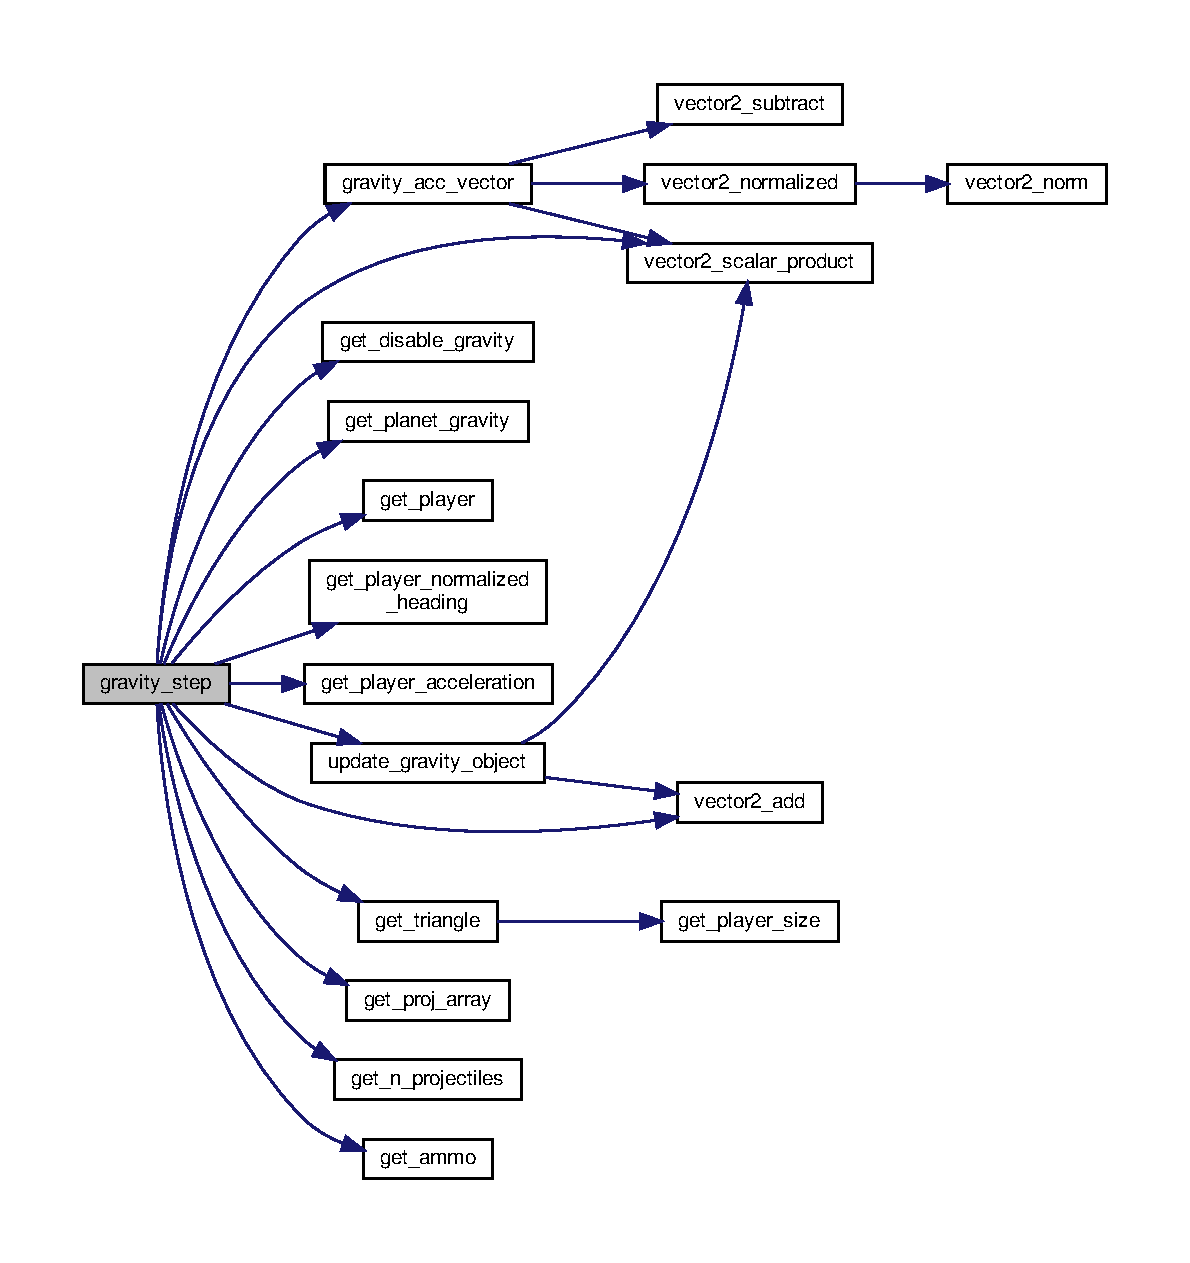
\includegraphics[width=350pt]{group__core__game__loop_ga46e6c6f53965490e91d8629d528ec797_cgraph}
\end{center}
\end{figure}
\mbox{\Hypertarget{group__core__game__loop_gac82e7d55ed069f5d0c396c20b97337e9}\label{group__core__game__loop_gac82e7d55ed069f5d0c396c20b97337e9}} 
\index{core\+\_\+game\+\_\+loop@{core\+\_\+game\+\_\+loop}!load\+\_\+xpms@{load\+\_\+xpms}}
\index{load\+\_\+xpms@{load\+\_\+xpms}!core\+\_\+game\+\_\+loop@{core\+\_\+game\+\_\+loop}}
\subsubsection{\texorpdfstring{load\+\_\+xpms()}{load\_xpms()}}
{\footnotesize\ttfamily void load\+\_\+xpms (\begin{DoxyParamCaption}{ }\end{DoxyParamCaption})}



Loads the X\+P\+Ms, if they have not been already loaded. 

\mbox{\Hypertarget{group__core__game__loop_gadffa4aa993db001bdee35fbce31dc00b}\label{group__core__game__loop_gadffa4aa993db001bdee35fbce31dc00b}} 
\index{core\+\_\+game\+\_\+loop@{core\+\_\+game\+\_\+loop}!player\+\_\+deal\+\_\+damage@{player\+\_\+deal\+\_\+damage}}
\index{player\+\_\+deal\+\_\+damage@{player\+\_\+deal\+\_\+damage}!core\+\_\+game\+\_\+loop@{core\+\_\+game\+\_\+loop}}
\subsubsection{\texorpdfstring{player\+\_\+deal\+\_\+damage()}{player\_deal\_damage()}}
{\footnotesize\ttfamily void player\+\_\+deal\+\_\+damage (\begin{DoxyParamCaption}\item[{uint8\+\_\+t}]{player,  }\item[{uint16\+\_\+t}]{damage }\end{DoxyParamCaption})}



Deals damage one of the players. If the player doesn\textquotesingle{}t have enough HP to take the hit, \hyperlink{group__core__game__loop_ga549153b90f3cb4e43291079eb5d893bf}{explode\+\_\+player(uint8\+\_\+t player)} is called and the game ends. 


\begin{DoxyParams}{Parameters}
{\em player} & The number of the player about to be damaged \\
\hline
{\em damage} & The amount of damage to be taken by the player, measured in pixels \\
\hline
\end{DoxyParams}
Here is the call graph for this function\+:\nopagebreak
\begin{figure}[H]
\begin{center}
\leavevmode
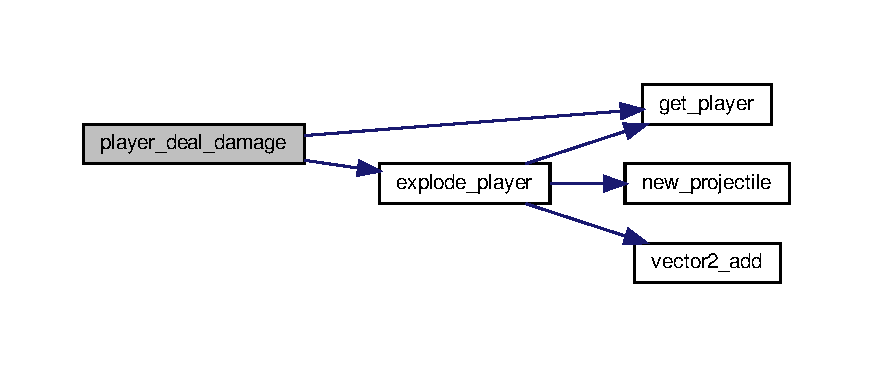
\includegraphics[width=350pt]{group__core__game__loop_gadffa4aa993db001bdee35fbce31dc00b_cgraph}
\end{center}
\end{figure}
\mbox{\Hypertarget{group__core__game__loop_ga7ffe05c55466ca7e6c94b73b63c22927}\label{group__core__game__loop_ga7ffe05c55466ca7e6c94b73b63c22927}} 
\index{core\+\_\+game\+\_\+loop@{core\+\_\+game\+\_\+loop}!player\+\_\+shoot@{player\+\_\+shoot}}
\index{player\+\_\+shoot@{player\+\_\+shoot}!core\+\_\+game\+\_\+loop@{core\+\_\+game\+\_\+loop}}
\subsubsection{\texorpdfstring{player\+\_\+shoot()}{player\_shoot()}}
{\footnotesize\ttfamily void player\+\_\+shoot (\begin{DoxyParamCaption}\item[{\hyperlink{structplayer}{player} $\ast$}]{p }\end{DoxyParamCaption})}



Spawns a projectile in front of p, with a given velocity. 


\begin{DoxyParams}{Parameters}
{\em p} & A pointer to the player that wants to shoot \\
\hline
\end{DoxyParams}
Here is the call graph for this function\+:\nopagebreak
\begin{figure}[H]
\begin{center}
\leavevmode
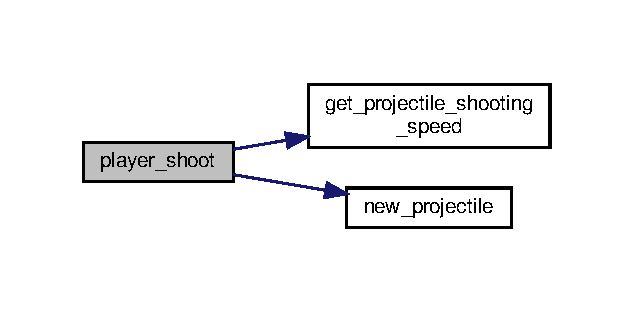
\includegraphics[width=304pt]{group__core__game__loop_ga7ffe05c55466ca7e6c94b73b63c22927_cgraph}
\end{center}
\end{figure}
\mbox{\Hypertarget{group__core__game__loop_ga79bddd8b336f6be116bfa658dd949e2e}\label{group__core__game__loop_ga79bddd8b336f6be116bfa658dd949e2e}} 
\index{core\+\_\+game\+\_\+loop@{core\+\_\+game\+\_\+loop}!shooting@{shooting}}
\index{shooting@{shooting}!core\+\_\+game\+\_\+loop@{core\+\_\+game\+\_\+loop}}
\subsubsection{\texorpdfstring{shooting()}{shooting()}}
{\footnotesize\ttfamily void shooting (\begin{DoxyParamCaption}{ }\end{DoxyParamCaption})}



The high-\/level shooting function. 

For each player it checks if the shooting conditions are met, and if so, calls \hyperlink{group__core__game__loop_ga7ffe05c55466ca7e6c94b73b63c22927}{player\+\_\+shoot(player $\ast$p)} Here is the call graph for this function\+:\nopagebreak
\begin{figure}[H]
\begin{center}
\leavevmode
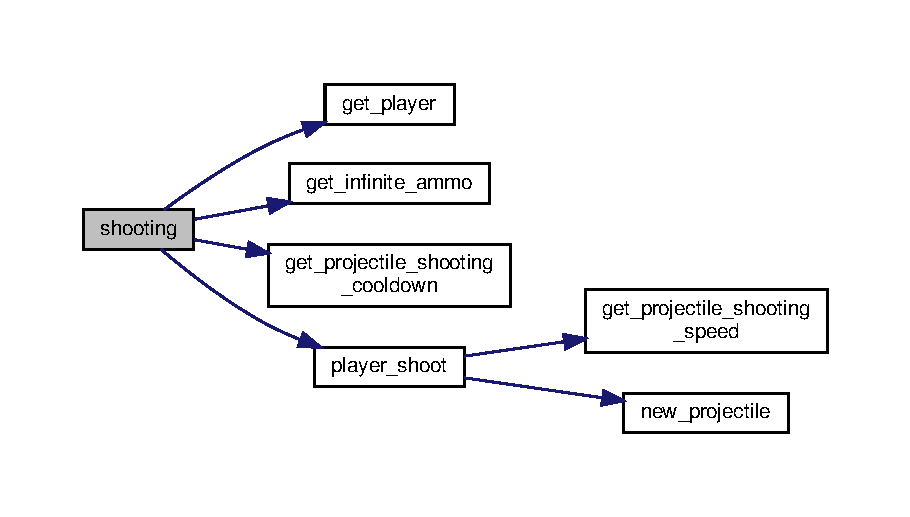
\includegraphics[width=350pt]{group__core__game__loop_ga79bddd8b336f6be116bfa658dd949e2e_cgraph}
\end{center}
\end{figure}

\hypertarget{group__core__game__settings}{}\section{core\+\_\+game\+\_\+settings}
\label{group__core__game__settings}\index{core\+\_\+game\+\_\+settings@{core\+\_\+game\+\_\+settings}}


Global settings that impact the way that core\+\_\+game\+\_\+loop runs.  


\subsection*{Functions}
\begin{DoxyCompactItemize}
\item 
uint16\+\_\+t \hyperlink{group__core__game__settings_gae7e72ac62497c693b7972e5b7aa2b42a}{get\+\_\+planet\+\_\+radius} ()
\item 
float \hyperlink{group__core__game__settings_ga7a058129c2abf0cc41fbd17f5265710d}{get\+\_\+planet\+\_\+gravity} ()
\item 
void \hyperlink{group__core__game__settings_ga9ad9d5a1de42dfd1bb9c35f918eb51ff}{set\+\_\+planet\+\_\+gravity} (float g)
\item 
float \hyperlink{group__core__game__settings_ga15eb947de263d29d6c97bae746737fa8}{get\+\_\+projectile\+\_\+shooting\+\_\+speed} ()
\item 
void \hyperlink{group__core__game__settings_ga5eeb5440c01178975630413285bee384}{set\+\_\+projectile\+\_\+shooting\+\_\+speed} (float speed)
\item 
uint8\+\_\+t \hyperlink{group__core__game__settings_ga10fcc8a3f6a22ea214e0b5e9f28362f8}{get\+\_\+projectile\+\_\+shooting\+\_\+cooldown} ()
\item 
void \hyperlink{group__core__game__settings_gaa78d2a1d2f17c5e37268f9b6d32ff885}{set\+\_\+projectile\+\_\+shooting\+\_\+cooldown} (uint8\+\_\+t cooldown)
\item 
uint32\+\_\+t \hyperlink{group__core__game__settings_ga0ba9dec3f44eebdfb14f0671b61f1b4e}{get\+\_\+projectile\+\_\+color} ()
\item 
void \hyperlink{group__core__game__settings_ga1d9f0dd4963fce752d49aea50e9c9d74}{set\+\_\+projectile\+\_\+color} (uint32\+\_\+t color)
\item 
uint32\+\_\+t \hyperlink{group__core__game__settings_ga614dd4319b2fe76e2a08747473836c0c}{get\+\_\+player1\+\_\+color} ()
\item 
void \hyperlink{group__core__game__settings_ga7d2df33bf9002ff71c661a521df4c279}{set\+\_\+player1\+\_\+color} (uint32\+\_\+t color)
\item 
uint32\+\_\+t \hyperlink{group__core__game__settings_gade5cf065ae24753f7fb8e73df7f8aa8f}{get\+\_\+player2\+\_\+color} ()
\item 
void \hyperlink{group__core__game__settings_ga03b1fe954023f0f81abcbf5e962e1169}{set\+\_\+player2\+\_\+color} (uint32\+\_\+t color)
\item 
float \hyperlink{group__core__game__settings_ga1eee074a8161cfbb24eab5bfab97369d}{get\+\_\+player\+\_\+size} ()
\item 
void \hyperlink{group__core__game__settings_ga0a444c4577d885de9a65789ed1f0a49e}{set\+\_\+player\+\_\+size} (float size)
\item 
float \hyperlink{group__core__game__settings_gaff00b21783e221feea599cb41520ebb8}{get\+\_\+player\+\_\+acceleration} ()
\item 
void \hyperlink{group__core__game__settings_gaf015b3fb5da34e2af0913a665b53f440}{set\+\_\+player\+\_\+acceleration} (float acc)
\item 
bool \hyperlink{group__core__game__settings_ga0288cff6bde3e658e0bea4e88a367039}{get\+\_\+bouncy\+\_\+walls} ()
\item 
void \hyperlink{group__core__game__settings_ga3d00a4e0dab9454c1176e82699a2d510}{set\+\_\+bouncy\+\_\+walls} (bool bouncy)
\item 
bool \hyperlink{group__core__game__settings_gae294ba27e3b2bf1d347ed563ee1327f7}{get\+\_\+disable\+\_\+gravity} ()
\item 
void \hyperlink{group__core__game__settings_gaef0357b1d6d13d5efcde0ebc880ef5ae}{set\+\_\+disable\+\_\+gravity} (bool disable)
\item 
bool \hyperlink{group__core__game__settings_gaf19a3bae554ca2a2ae3213aef7f9f208}{get\+\_\+infinite\+\_\+ammo} ()
\item 
void \hyperlink{group__core__game__settings_ga098db2a1aea09dead03ad58bb667bff9}{set\+\_\+infinite\+\_\+ammo} (bool infinite)
\item 
bool \hyperlink{group__core__game__settings_gae98ea18abc06d0d144350c2c6018bdb9}{get\+\_\+disable\+\_\+wall\+\_\+damage} ()
\item 
void \hyperlink{group__core__game__settings_gaf4298289f3e03eb97347eb6a3865ec60}{set\+\_\+disable\+\_\+wall\+\_\+damage} (bool damage)
\end{DoxyCompactItemize}


\subsection{Detailed Description}
Global settings that impact the way that core\+\_\+game\+\_\+loop runs. 



\subsection{Function Documentation}
\mbox{\Hypertarget{group__core__game__settings_ga0288cff6bde3e658e0bea4e88a367039}\label{group__core__game__settings_ga0288cff6bde3e658e0bea4e88a367039}} 
\index{core\+\_\+game\+\_\+settings@{core\+\_\+game\+\_\+settings}!get\+\_\+bouncy\+\_\+walls@{get\+\_\+bouncy\+\_\+walls}}
\index{get\+\_\+bouncy\+\_\+walls@{get\+\_\+bouncy\+\_\+walls}!core\+\_\+game\+\_\+settings@{core\+\_\+game\+\_\+settings}}
\subsubsection{\texorpdfstring{get\+\_\+bouncy\+\_\+walls()}{get\_bouncy\_walls()}}
{\footnotesize\ttfamily bool get\+\_\+bouncy\+\_\+walls (\begin{DoxyParamCaption}{ }\end{DoxyParamCaption})}

\begin{DoxyReturn}{Returns}
Whether or not projectiles bounce back from the walls of the screen 
\end{DoxyReturn}
\mbox{\Hypertarget{group__core__game__settings_gae294ba27e3b2bf1d347ed563ee1327f7}\label{group__core__game__settings_gae294ba27e3b2bf1d347ed563ee1327f7}} 
\index{core\+\_\+game\+\_\+settings@{core\+\_\+game\+\_\+settings}!get\+\_\+disable\+\_\+gravity@{get\+\_\+disable\+\_\+gravity}}
\index{get\+\_\+disable\+\_\+gravity@{get\+\_\+disable\+\_\+gravity}!core\+\_\+game\+\_\+settings@{core\+\_\+game\+\_\+settings}}
\subsubsection{\texorpdfstring{get\+\_\+disable\+\_\+gravity()}{get\_disable\_gravity()}}
{\footnotesize\ttfamily bool get\+\_\+disable\+\_\+gravity (\begin{DoxyParamCaption}{ }\end{DoxyParamCaption})}

\begin{DoxyReturn}{Returns}
Whether or not gravity is disabled 
\end{DoxyReturn}
\mbox{\Hypertarget{group__core__game__settings_gae98ea18abc06d0d144350c2c6018bdb9}\label{group__core__game__settings_gae98ea18abc06d0d144350c2c6018bdb9}} 
\index{core\+\_\+game\+\_\+settings@{core\+\_\+game\+\_\+settings}!get\+\_\+disable\+\_\+wall\+\_\+damage@{get\+\_\+disable\+\_\+wall\+\_\+damage}}
\index{get\+\_\+disable\+\_\+wall\+\_\+damage@{get\+\_\+disable\+\_\+wall\+\_\+damage}!core\+\_\+game\+\_\+settings@{core\+\_\+game\+\_\+settings}}
\subsubsection{\texorpdfstring{get\+\_\+disable\+\_\+wall\+\_\+damage()}{get\_disable\_wall\_damage()}}
{\footnotesize\ttfamily bool get\+\_\+disable\+\_\+wall\+\_\+damage (\begin{DoxyParamCaption}{ }\end{DoxyParamCaption})}

\begin{DoxyReturn}{Returns}
Whether or not wall damage is disabled 
\end{DoxyReturn}
\mbox{\Hypertarget{group__core__game__settings_gaf19a3bae554ca2a2ae3213aef7f9f208}\label{group__core__game__settings_gaf19a3bae554ca2a2ae3213aef7f9f208}} 
\index{core\+\_\+game\+\_\+settings@{core\+\_\+game\+\_\+settings}!get\+\_\+infinite\+\_\+ammo@{get\+\_\+infinite\+\_\+ammo}}
\index{get\+\_\+infinite\+\_\+ammo@{get\+\_\+infinite\+\_\+ammo}!core\+\_\+game\+\_\+settings@{core\+\_\+game\+\_\+settings}}
\subsubsection{\texorpdfstring{get\+\_\+infinite\+\_\+ammo()}{get\_infinite\_ammo()}}
{\footnotesize\ttfamily bool get\+\_\+infinite\+\_\+ammo (\begin{DoxyParamCaption}{ }\end{DoxyParamCaption})}

\begin{DoxyReturn}{Returns}
Whether or not infinite ammo is enabled 
\end{DoxyReturn}
\mbox{\Hypertarget{group__core__game__settings_ga7a058129c2abf0cc41fbd17f5265710d}\label{group__core__game__settings_ga7a058129c2abf0cc41fbd17f5265710d}} 
\index{core\+\_\+game\+\_\+settings@{core\+\_\+game\+\_\+settings}!get\+\_\+planet\+\_\+gravity@{get\+\_\+planet\+\_\+gravity}}
\index{get\+\_\+planet\+\_\+gravity@{get\+\_\+planet\+\_\+gravity}!core\+\_\+game\+\_\+settings@{core\+\_\+game\+\_\+settings}}
\subsubsection{\texorpdfstring{get\+\_\+planet\+\_\+gravity()}{get\_planet\_gravity()}}
{\footnotesize\ttfamily float get\+\_\+planet\+\_\+gravity (\begin{DoxyParamCaption}{ }\end{DoxyParamCaption})}

\begin{DoxyReturn}{Returns}
The \href{https://en.wikipedia.org/wiki/Standard_gravitational_parameter}{\tt gravitational parameter} of the planet 
\end{DoxyReturn}
\mbox{\Hypertarget{group__core__game__settings_gae7e72ac62497c693b7972e5b7aa2b42a}\label{group__core__game__settings_gae7e72ac62497c693b7972e5b7aa2b42a}} 
\index{core\+\_\+game\+\_\+settings@{core\+\_\+game\+\_\+settings}!get\+\_\+planet\+\_\+radius@{get\+\_\+planet\+\_\+radius}}
\index{get\+\_\+planet\+\_\+radius@{get\+\_\+planet\+\_\+radius}!core\+\_\+game\+\_\+settings@{core\+\_\+game\+\_\+settings}}
\subsubsection{\texorpdfstring{get\+\_\+planet\+\_\+radius()}{get\_planet\_radius()}}
{\footnotesize\ttfamily uint16\+\_\+t get\+\_\+planet\+\_\+radius (\begin{DoxyParamCaption}{ }\end{DoxyParamCaption})}

\begin{DoxyReturn}{Returns}
The radius of the planet, in pixels 
\end{DoxyReturn}
\mbox{\Hypertarget{group__core__game__settings_ga614dd4319b2fe76e2a08747473836c0c}\label{group__core__game__settings_ga614dd4319b2fe76e2a08747473836c0c}} 
\index{core\+\_\+game\+\_\+settings@{core\+\_\+game\+\_\+settings}!get\+\_\+player1\+\_\+color@{get\+\_\+player1\+\_\+color}}
\index{get\+\_\+player1\+\_\+color@{get\+\_\+player1\+\_\+color}!core\+\_\+game\+\_\+settings@{core\+\_\+game\+\_\+settings}}
\subsubsection{\texorpdfstring{get\+\_\+player1\+\_\+color()}{get\_player1\_color()}}
{\footnotesize\ttfamily uint32\+\_\+t get\+\_\+player1\+\_\+color (\begin{DoxyParamCaption}{ }\end{DoxyParamCaption})}

\begin{DoxyReturn}{Returns}
The color of player 1 
\end{DoxyReturn}
\mbox{\Hypertarget{group__core__game__settings_gade5cf065ae24753f7fb8e73df7f8aa8f}\label{group__core__game__settings_gade5cf065ae24753f7fb8e73df7f8aa8f}} 
\index{core\+\_\+game\+\_\+settings@{core\+\_\+game\+\_\+settings}!get\+\_\+player2\+\_\+color@{get\+\_\+player2\+\_\+color}}
\index{get\+\_\+player2\+\_\+color@{get\+\_\+player2\+\_\+color}!core\+\_\+game\+\_\+settings@{core\+\_\+game\+\_\+settings}}
\subsubsection{\texorpdfstring{get\+\_\+player2\+\_\+color()}{get\_player2\_color()}}
{\footnotesize\ttfamily uint32\+\_\+t get\+\_\+player2\+\_\+color (\begin{DoxyParamCaption}{ }\end{DoxyParamCaption})}

\begin{DoxyReturn}{Returns}
The color of player 2 
\end{DoxyReturn}
\mbox{\Hypertarget{group__core__game__settings_gaff00b21783e221feea599cb41520ebb8}\label{group__core__game__settings_gaff00b21783e221feea599cb41520ebb8}} 
\index{core\+\_\+game\+\_\+settings@{core\+\_\+game\+\_\+settings}!get\+\_\+player\+\_\+acceleration@{get\+\_\+player\+\_\+acceleration}}
\index{get\+\_\+player\+\_\+acceleration@{get\+\_\+player\+\_\+acceleration}!core\+\_\+game\+\_\+settings@{core\+\_\+game\+\_\+settings}}
\subsubsection{\texorpdfstring{get\+\_\+player\+\_\+acceleration()}{get\_player\_acceleration()}}
{\footnotesize\ttfamily float get\+\_\+player\+\_\+acceleration (\begin{DoxyParamCaption}{ }\end{DoxyParamCaption})}

\begin{DoxyReturn}{Returns}
The players\textquotesingle{} acceleration 
\end{DoxyReturn}
\mbox{\Hypertarget{group__core__game__settings_ga1eee074a8161cfbb24eab5bfab97369d}\label{group__core__game__settings_ga1eee074a8161cfbb24eab5bfab97369d}} 
\index{core\+\_\+game\+\_\+settings@{core\+\_\+game\+\_\+settings}!get\+\_\+player\+\_\+size@{get\+\_\+player\+\_\+size}}
\index{get\+\_\+player\+\_\+size@{get\+\_\+player\+\_\+size}!core\+\_\+game\+\_\+settings@{core\+\_\+game\+\_\+settings}}
\subsubsection{\texorpdfstring{get\+\_\+player\+\_\+size()}{get\_player\_size()}}
{\footnotesize\ttfamily float get\+\_\+player\+\_\+size (\begin{DoxyParamCaption}{ }\end{DoxyParamCaption})}

\begin{DoxyReturn}{Returns}
The players\textquotesingle{} size 
\end{DoxyReturn}
\mbox{\Hypertarget{group__core__game__settings_ga0ba9dec3f44eebdfb14f0671b61f1b4e}\label{group__core__game__settings_ga0ba9dec3f44eebdfb14f0671b61f1b4e}} 
\index{core\+\_\+game\+\_\+settings@{core\+\_\+game\+\_\+settings}!get\+\_\+projectile\+\_\+color@{get\+\_\+projectile\+\_\+color}}
\index{get\+\_\+projectile\+\_\+color@{get\+\_\+projectile\+\_\+color}!core\+\_\+game\+\_\+settings@{core\+\_\+game\+\_\+settings}}
\subsubsection{\texorpdfstring{get\+\_\+projectile\+\_\+color()}{get\_projectile\_color()}}
{\footnotesize\ttfamily uint32\+\_\+t get\+\_\+projectile\+\_\+color (\begin{DoxyParamCaption}{ }\end{DoxyParamCaption})}

\begin{DoxyReturn}{Returns}
The color of the projectiles 
\end{DoxyReturn}
\mbox{\Hypertarget{group__core__game__settings_ga10fcc8a3f6a22ea214e0b5e9f28362f8}\label{group__core__game__settings_ga10fcc8a3f6a22ea214e0b5e9f28362f8}} 
\index{core\+\_\+game\+\_\+settings@{core\+\_\+game\+\_\+settings}!get\+\_\+projectile\+\_\+shooting\+\_\+cooldown@{get\+\_\+projectile\+\_\+shooting\+\_\+cooldown}}
\index{get\+\_\+projectile\+\_\+shooting\+\_\+cooldown@{get\+\_\+projectile\+\_\+shooting\+\_\+cooldown}!core\+\_\+game\+\_\+settings@{core\+\_\+game\+\_\+settings}}
\subsubsection{\texorpdfstring{get\+\_\+projectile\+\_\+shooting\+\_\+cooldown()}{get\_projectile\_shooting\_cooldown()}}
{\footnotesize\ttfamily uint8\+\_\+t get\+\_\+projectile\+\_\+shooting\+\_\+cooldown (\begin{DoxyParamCaption}{ }\end{DoxyParamCaption})}

\begin{DoxyReturn}{Returns}
The numbers of frames between two shots 
\end{DoxyReturn}
\mbox{\Hypertarget{group__core__game__settings_ga15eb947de263d29d6c97bae746737fa8}\label{group__core__game__settings_ga15eb947de263d29d6c97bae746737fa8}} 
\index{core\+\_\+game\+\_\+settings@{core\+\_\+game\+\_\+settings}!get\+\_\+projectile\+\_\+shooting\+\_\+speed@{get\+\_\+projectile\+\_\+shooting\+\_\+speed}}
\index{get\+\_\+projectile\+\_\+shooting\+\_\+speed@{get\+\_\+projectile\+\_\+shooting\+\_\+speed}!core\+\_\+game\+\_\+settings@{core\+\_\+game\+\_\+settings}}
\subsubsection{\texorpdfstring{get\+\_\+projectile\+\_\+shooting\+\_\+speed()}{get\_projectile\_shooting\_speed()}}
{\footnotesize\ttfamily float get\+\_\+projectile\+\_\+shooting\+\_\+speed (\begin{DoxyParamCaption}{ }\end{DoxyParamCaption})}

\begin{DoxyReturn}{Returns}
The velocity at which the projectile exits the player 
\end{DoxyReturn}
\mbox{\Hypertarget{group__core__game__settings_ga3d00a4e0dab9454c1176e82699a2d510}\label{group__core__game__settings_ga3d00a4e0dab9454c1176e82699a2d510}} 
\index{core\+\_\+game\+\_\+settings@{core\+\_\+game\+\_\+settings}!set\+\_\+bouncy\+\_\+walls@{set\+\_\+bouncy\+\_\+walls}}
\index{set\+\_\+bouncy\+\_\+walls@{set\+\_\+bouncy\+\_\+walls}!core\+\_\+game\+\_\+settings@{core\+\_\+game\+\_\+settings}}
\subsubsection{\texorpdfstring{set\+\_\+bouncy\+\_\+walls()}{set\_bouncy\_walls()}}
{\footnotesize\ttfamily void set\+\_\+bouncy\+\_\+walls (\begin{DoxyParamCaption}\item[{bool}]{bouncy }\end{DoxyParamCaption})}


\begin{DoxyParams}{Parameters}
{\em bouncy} & Whether or not projectiles bounce back from the walls of the screen \\
\hline
\end{DoxyParams}
\mbox{\Hypertarget{group__core__game__settings_gaef0357b1d6d13d5efcde0ebc880ef5ae}\label{group__core__game__settings_gaef0357b1d6d13d5efcde0ebc880ef5ae}} 
\index{core\+\_\+game\+\_\+settings@{core\+\_\+game\+\_\+settings}!set\+\_\+disable\+\_\+gravity@{set\+\_\+disable\+\_\+gravity}}
\index{set\+\_\+disable\+\_\+gravity@{set\+\_\+disable\+\_\+gravity}!core\+\_\+game\+\_\+settings@{core\+\_\+game\+\_\+settings}}
\subsubsection{\texorpdfstring{set\+\_\+disable\+\_\+gravity()}{set\_disable\_gravity()}}
{\footnotesize\ttfamily void set\+\_\+disable\+\_\+gravity (\begin{DoxyParamCaption}\item[{bool}]{disable }\end{DoxyParamCaption})}


\begin{DoxyParams}{Parameters}
{\em disable} & Whether or not gravity is disabled \\
\hline
\end{DoxyParams}
\mbox{\Hypertarget{group__core__game__settings_gaf4298289f3e03eb97347eb6a3865ec60}\label{group__core__game__settings_gaf4298289f3e03eb97347eb6a3865ec60}} 
\index{core\+\_\+game\+\_\+settings@{core\+\_\+game\+\_\+settings}!set\+\_\+disable\+\_\+wall\+\_\+damage@{set\+\_\+disable\+\_\+wall\+\_\+damage}}
\index{set\+\_\+disable\+\_\+wall\+\_\+damage@{set\+\_\+disable\+\_\+wall\+\_\+damage}!core\+\_\+game\+\_\+settings@{core\+\_\+game\+\_\+settings}}
\subsubsection{\texorpdfstring{set\+\_\+disable\+\_\+wall\+\_\+damage()}{set\_disable\_wall\_damage()}}
{\footnotesize\ttfamily void set\+\_\+disable\+\_\+wall\+\_\+damage (\begin{DoxyParamCaption}\item[{bool}]{damage }\end{DoxyParamCaption})}


\begin{DoxyParams}{Parameters}
{\em damage} & Whether or not wall damage is disabled \\
\hline
\end{DoxyParams}
\mbox{\Hypertarget{group__core__game__settings_ga098db2a1aea09dead03ad58bb667bff9}\label{group__core__game__settings_ga098db2a1aea09dead03ad58bb667bff9}} 
\index{core\+\_\+game\+\_\+settings@{core\+\_\+game\+\_\+settings}!set\+\_\+infinite\+\_\+ammo@{set\+\_\+infinite\+\_\+ammo}}
\index{set\+\_\+infinite\+\_\+ammo@{set\+\_\+infinite\+\_\+ammo}!core\+\_\+game\+\_\+settings@{core\+\_\+game\+\_\+settings}}
\subsubsection{\texorpdfstring{set\+\_\+infinite\+\_\+ammo()}{set\_infinite\_ammo()}}
{\footnotesize\ttfamily void set\+\_\+infinite\+\_\+ammo (\begin{DoxyParamCaption}\item[{bool}]{infinite }\end{DoxyParamCaption})}


\begin{DoxyParams}{Parameters}
{\em infinite} & Whether or not infinite ammo is enabled \\
\hline
\end{DoxyParams}
\mbox{\Hypertarget{group__core__game__settings_ga9ad9d5a1de42dfd1bb9c35f918eb51ff}\label{group__core__game__settings_ga9ad9d5a1de42dfd1bb9c35f918eb51ff}} 
\index{core\+\_\+game\+\_\+settings@{core\+\_\+game\+\_\+settings}!set\+\_\+planet\+\_\+gravity@{set\+\_\+planet\+\_\+gravity}}
\index{set\+\_\+planet\+\_\+gravity@{set\+\_\+planet\+\_\+gravity}!core\+\_\+game\+\_\+settings@{core\+\_\+game\+\_\+settings}}
\subsubsection{\texorpdfstring{set\+\_\+planet\+\_\+gravity()}{set\_planet\_gravity()}}
{\footnotesize\ttfamily void set\+\_\+planet\+\_\+gravity (\begin{DoxyParamCaption}\item[{float}]{g }\end{DoxyParamCaption})}


\begin{DoxyParams}{Parameters}
{\em g} & The \href{https://en.wikipedia.org/wiki/Standard_gravitational_parameter}{\tt gravitational parameter} of the planet \\
\hline
\end{DoxyParams}
\mbox{\Hypertarget{group__core__game__settings_ga7d2df33bf9002ff71c661a521df4c279}\label{group__core__game__settings_ga7d2df33bf9002ff71c661a521df4c279}} 
\index{core\+\_\+game\+\_\+settings@{core\+\_\+game\+\_\+settings}!set\+\_\+player1\+\_\+color@{set\+\_\+player1\+\_\+color}}
\index{set\+\_\+player1\+\_\+color@{set\+\_\+player1\+\_\+color}!core\+\_\+game\+\_\+settings@{core\+\_\+game\+\_\+settings}}
\subsubsection{\texorpdfstring{set\+\_\+player1\+\_\+color()}{set\_player1\_color()}}
{\footnotesize\ttfamily void set\+\_\+player1\+\_\+color (\begin{DoxyParamCaption}\item[{uint32\+\_\+t}]{color }\end{DoxyParamCaption})}


\begin{DoxyParams}{Parameters}
{\em color} & The color of player 1 \\
\hline
\end{DoxyParams}
\mbox{\Hypertarget{group__core__game__settings_ga03b1fe954023f0f81abcbf5e962e1169}\label{group__core__game__settings_ga03b1fe954023f0f81abcbf5e962e1169}} 
\index{core\+\_\+game\+\_\+settings@{core\+\_\+game\+\_\+settings}!set\+\_\+player2\+\_\+color@{set\+\_\+player2\+\_\+color}}
\index{set\+\_\+player2\+\_\+color@{set\+\_\+player2\+\_\+color}!core\+\_\+game\+\_\+settings@{core\+\_\+game\+\_\+settings}}
\subsubsection{\texorpdfstring{set\+\_\+player2\+\_\+color()}{set\_player2\_color()}}
{\footnotesize\ttfamily void set\+\_\+player2\+\_\+color (\begin{DoxyParamCaption}\item[{uint32\+\_\+t}]{color }\end{DoxyParamCaption})}


\begin{DoxyParams}{Parameters}
{\em color} & The color of player 2 \\
\hline
\end{DoxyParams}
\mbox{\Hypertarget{group__core__game__settings_gaf015b3fb5da34e2af0913a665b53f440}\label{group__core__game__settings_gaf015b3fb5da34e2af0913a665b53f440}} 
\index{core\+\_\+game\+\_\+settings@{core\+\_\+game\+\_\+settings}!set\+\_\+player\+\_\+acceleration@{set\+\_\+player\+\_\+acceleration}}
\index{set\+\_\+player\+\_\+acceleration@{set\+\_\+player\+\_\+acceleration}!core\+\_\+game\+\_\+settings@{core\+\_\+game\+\_\+settings}}
\subsubsection{\texorpdfstring{set\+\_\+player\+\_\+acceleration()}{set\_player\_acceleration()}}
{\footnotesize\ttfamily void set\+\_\+player\+\_\+acceleration (\begin{DoxyParamCaption}\item[{float}]{acc }\end{DoxyParamCaption})}


\begin{DoxyParams}{Parameters}
{\em acc} & The players\textquotesingle{} acceleration \\
\hline
\end{DoxyParams}
\mbox{\Hypertarget{group__core__game__settings_ga0a444c4577d885de9a65789ed1f0a49e}\label{group__core__game__settings_ga0a444c4577d885de9a65789ed1f0a49e}} 
\index{core\+\_\+game\+\_\+settings@{core\+\_\+game\+\_\+settings}!set\+\_\+player\+\_\+size@{set\+\_\+player\+\_\+size}}
\index{set\+\_\+player\+\_\+size@{set\+\_\+player\+\_\+size}!core\+\_\+game\+\_\+settings@{core\+\_\+game\+\_\+settings}}
\subsubsection{\texorpdfstring{set\+\_\+player\+\_\+size()}{set\_player\_size()}}
{\footnotesize\ttfamily void set\+\_\+player\+\_\+size (\begin{DoxyParamCaption}\item[{float}]{size }\end{DoxyParamCaption})}


\begin{DoxyParams}{Parameters}
{\em size} & The players\textquotesingle{} size \\
\hline
\end{DoxyParams}
\mbox{\Hypertarget{group__core__game__settings_ga1d9f0dd4963fce752d49aea50e9c9d74}\label{group__core__game__settings_ga1d9f0dd4963fce752d49aea50e9c9d74}} 
\index{core\+\_\+game\+\_\+settings@{core\+\_\+game\+\_\+settings}!set\+\_\+projectile\+\_\+color@{set\+\_\+projectile\+\_\+color}}
\index{set\+\_\+projectile\+\_\+color@{set\+\_\+projectile\+\_\+color}!core\+\_\+game\+\_\+settings@{core\+\_\+game\+\_\+settings}}
\subsubsection{\texorpdfstring{set\+\_\+projectile\+\_\+color()}{set\_projectile\_color()}}
{\footnotesize\ttfamily void set\+\_\+projectile\+\_\+color (\begin{DoxyParamCaption}\item[{uint32\+\_\+t}]{color }\end{DoxyParamCaption})}


\begin{DoxyParams}{Parameters}
{\em color} & The color of the projectiles \\
\hline
\end{DoxyParams}
\mbox{\Hypertarget{group__core__game__settings_gaa78d2a1d2f17c5e37268f9b6d32ff885}\label{group__core__game__settings_gaa78d2a1d2f17c5e37268f9b6d32ff885}} 
\index{core\+\_\+game\+\_\+settings@{core\+\_\+game\+\_\+settings}!set\+\_\+projectile\+\_\+shooting\+\_\+cooldown@{set\+\_\+projectile\+\_\+shooting\+\_\+cooldown}}
\index{set\+\_\+projectile\+\_\+shooting\+\_\+cooldown@{set\+\_\+projectile\+\_\+shooting\+\_\+cooldown}!core\+\_\+game\+\_\+settings@{core\+\_\+game\+\_\+settings}}
\subsubsection{\texorpdfstring{set\+\_\+projectile\+\_\+shooting\+\_\+cooldown()}{set\_projectile\_shooting\_cooldown()}}
{\footnotesize\ttfamily void set\+\_\+projectile\+\_\+shooting\+\_\+cooldown (\begin{DoxyParamCaption}\item[{uint8\+\_\+t}]{cooldown }\end{DoxyParamCaption})}


\begin{DoxyParams}{Parameters}
{\em cooldown} & The numbers of frames between two shots \\
\hline
\end{DoxyParams}
\mbox{\Hypertarget{group__core__game__settings_ga5eeb5440c01178975630413285bee384}\label{group__core__game__settings_ga5eeb5440c01178975630413285bee384}} 
\index{core\+\_\+game\+\_\+settings@{core\+\_\+game\+\_\+settings}!set\+\_\+projectile\+\_\+shooting\+\_\+speed@{set\+\_\+projectile\+\_\+shooting\+\_\+speed}}
\index{set\+\_\+projectile\+\_\+shooting\+\_\+speed@{set\+\_\+projectile\+\_\+shooting\+\_\+speed}!core\+\_\+game\+\_\+settings@{core\+\_\+game\+\_\+settings}}
\subsubsection{\texorpdfstring{set\+\_\+projectile\+\_\+shooting\+\_\+speed()}{set\_projectile\_shooting\_speed()}}
{\footnotesize\ttfamily void set\+\_\+projectile\+\_\+shooting\+\_\+speed (\begin{DoxyParamCaption}\item[{float}]{speed }\end{DoxyParamCaption})}


\begin{DoxyParams}{Parameters}
{\em speed} & The velocity at which the projectile exits the player \\
\hline
\end{DoxyParams}

\hypertarget{group__game}{}\section{game}
\label{group__game}\index{game@{game}}


game-\/related functions  


\subsection*{Functions}
\begin{DoxyCompactItemize}
\item 
void \hyperlink{group__game_gac443369f029f95734396be718a095e93}{handle\+\_\+user\+\_\+input} (\hyperlink{structmouse__packet}{mouse\+\_\+packet} p1)
\item 
void \hyperlink{group__game_gae53a2c47c7b05d012ce5356a53ae7092}{handle\+\_\+state} ()
\item 
void \hyperlink{group__game_ga435b545b95a32afd525f8a1f05b2652c}{letsplay} ()
\end{DoxyCompactItemize}


\subsection{Detailed Description}
game-\/related functions 



\subsection{Function Documentation}
\mbox{\Hypertarget{group__game_gae53a2c47c7b05d012ce5356a53ae7092}\label{group__game_gae53a2c47c7b05d012ce5356a53ae7092}} 
\index{game@{game}!handle\+\_\+state@{handle\+\_\+state}}
\index{handle\+\_\+state@{handle\+\_\+state}!game@{game}}
\subsubsection{\texorpdfstring{handle\+\_\+state()}{handle\_state()}}
{\footnotesize\ttfamily void handle\+\_\+state (\begin{DoxyParamCaption}{ }\end{DoxyParamCaption})}

Here is the call graph for this function\+:
\nopagebreak
\begin{figure}[H]
\begin{center}
\leavevmode
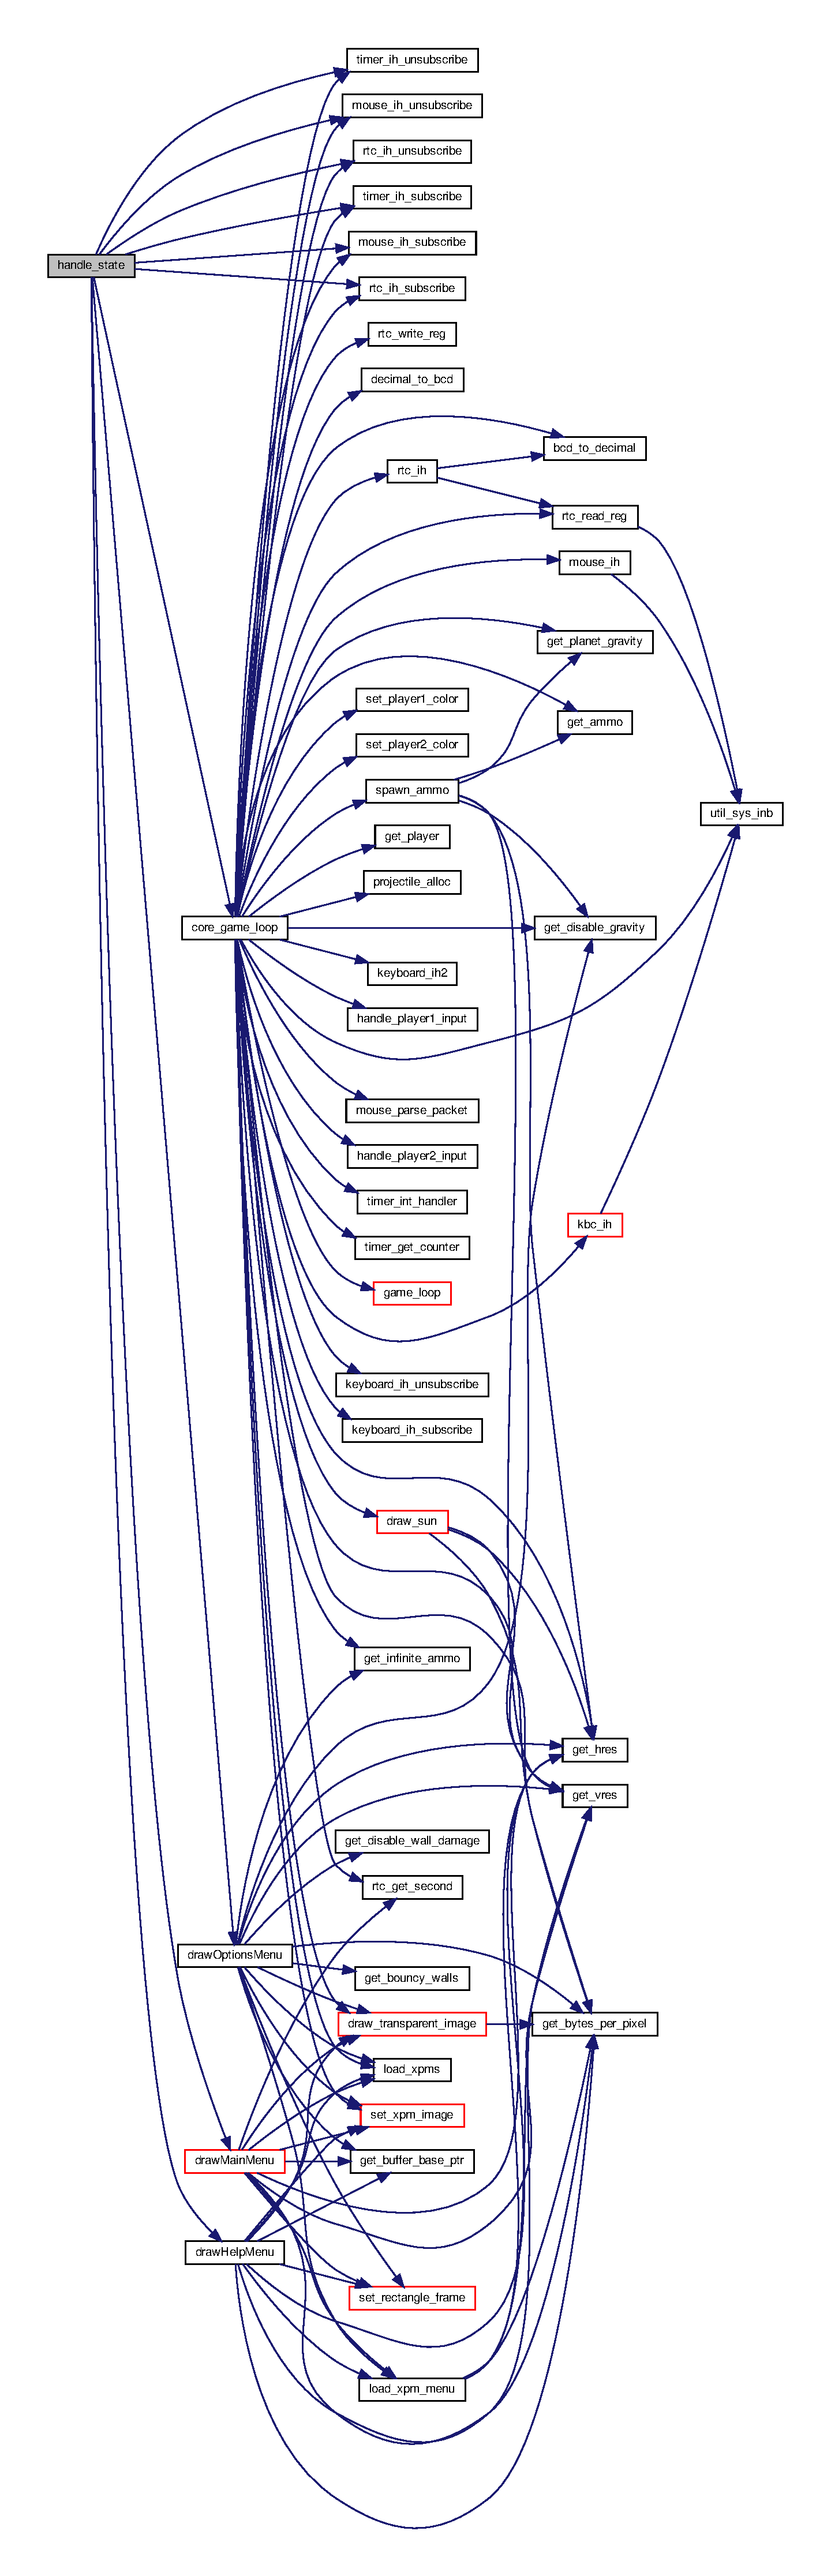
\includegraphics[height=550pt]{group__game_gae53a2c47c7b05d012ce5356a53ae7092_cgraph}
\end{center}
\end{figure}
\mbox{\Hypertarget{group__game_gac443369f029f95734396be718a095e93}\label{group__game_gac443369f029f95734396be718a095e93}} 
\index{game@{game}!handle\+\_\+user\+\_\+input@{handle\+\_\+user\+\_\+input}}
\index{handle\+\_\+user\+\_\+input@{handle\+\_\+user\+\_\+input}!game@{game}}
\subsubsection{\texorpdfstring{handle\+\_\+user\+\_\+input()}{handle\_user\_input()}}
{\footnotesize\ttfamily void handle\+\_\+user\+\_\+input (\begin{DoxyParamCaption}\item[{\hyperlink{structmouse__packet}{mouse\+\_\+packet}}]{p1 }\end{DoxyParamCaption})}

Here is the call graph for this function\+:\nopagebreak
\begin{figure}[H]
\begin{center}
\leavevmode
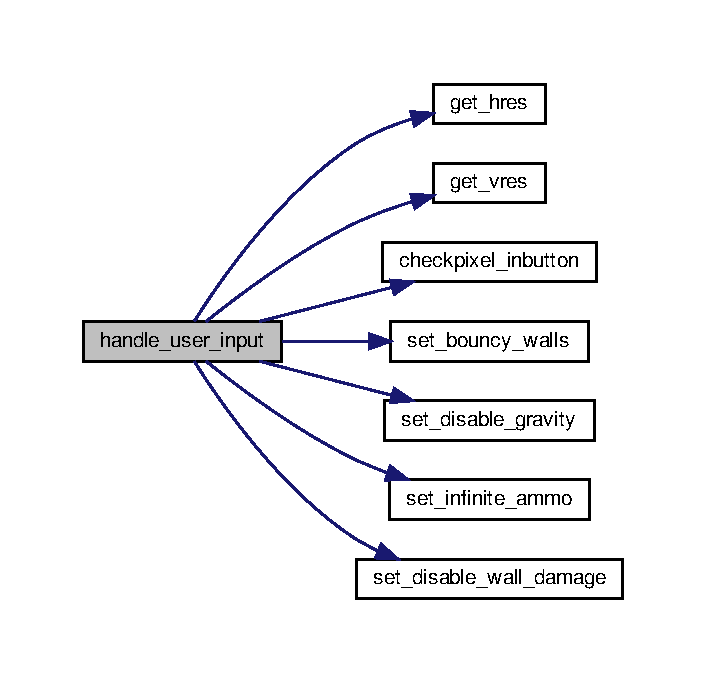
\includegraphics[width=339pt]{group__game_gac443369f029f95734396be718a095e93_cgraph}
\end{center}
\end{figure}
\mbox{\Hypertarget{group__game_ga435b545b95a32afd525f8a1f05b2652c}\label{group__game_ga435b545b95a32afd525f8a1f05b2652c}} 
\index{game@{game}!letsplay@{letsplay}}
\index{letsplay@{letsplay}!game@{game}}
\subsubsection{\texorpdfstring{letsplay()}{letsplay()}}
{\footnotesize\ttfamily void letsplay (\begin{DoxyParamCaption}{ }\end{DoxyParamCaption})}

Here is the call graph for this function\+:
\nopagebreak
\begin{figure}[H]
\begin{center}
\leavevmode
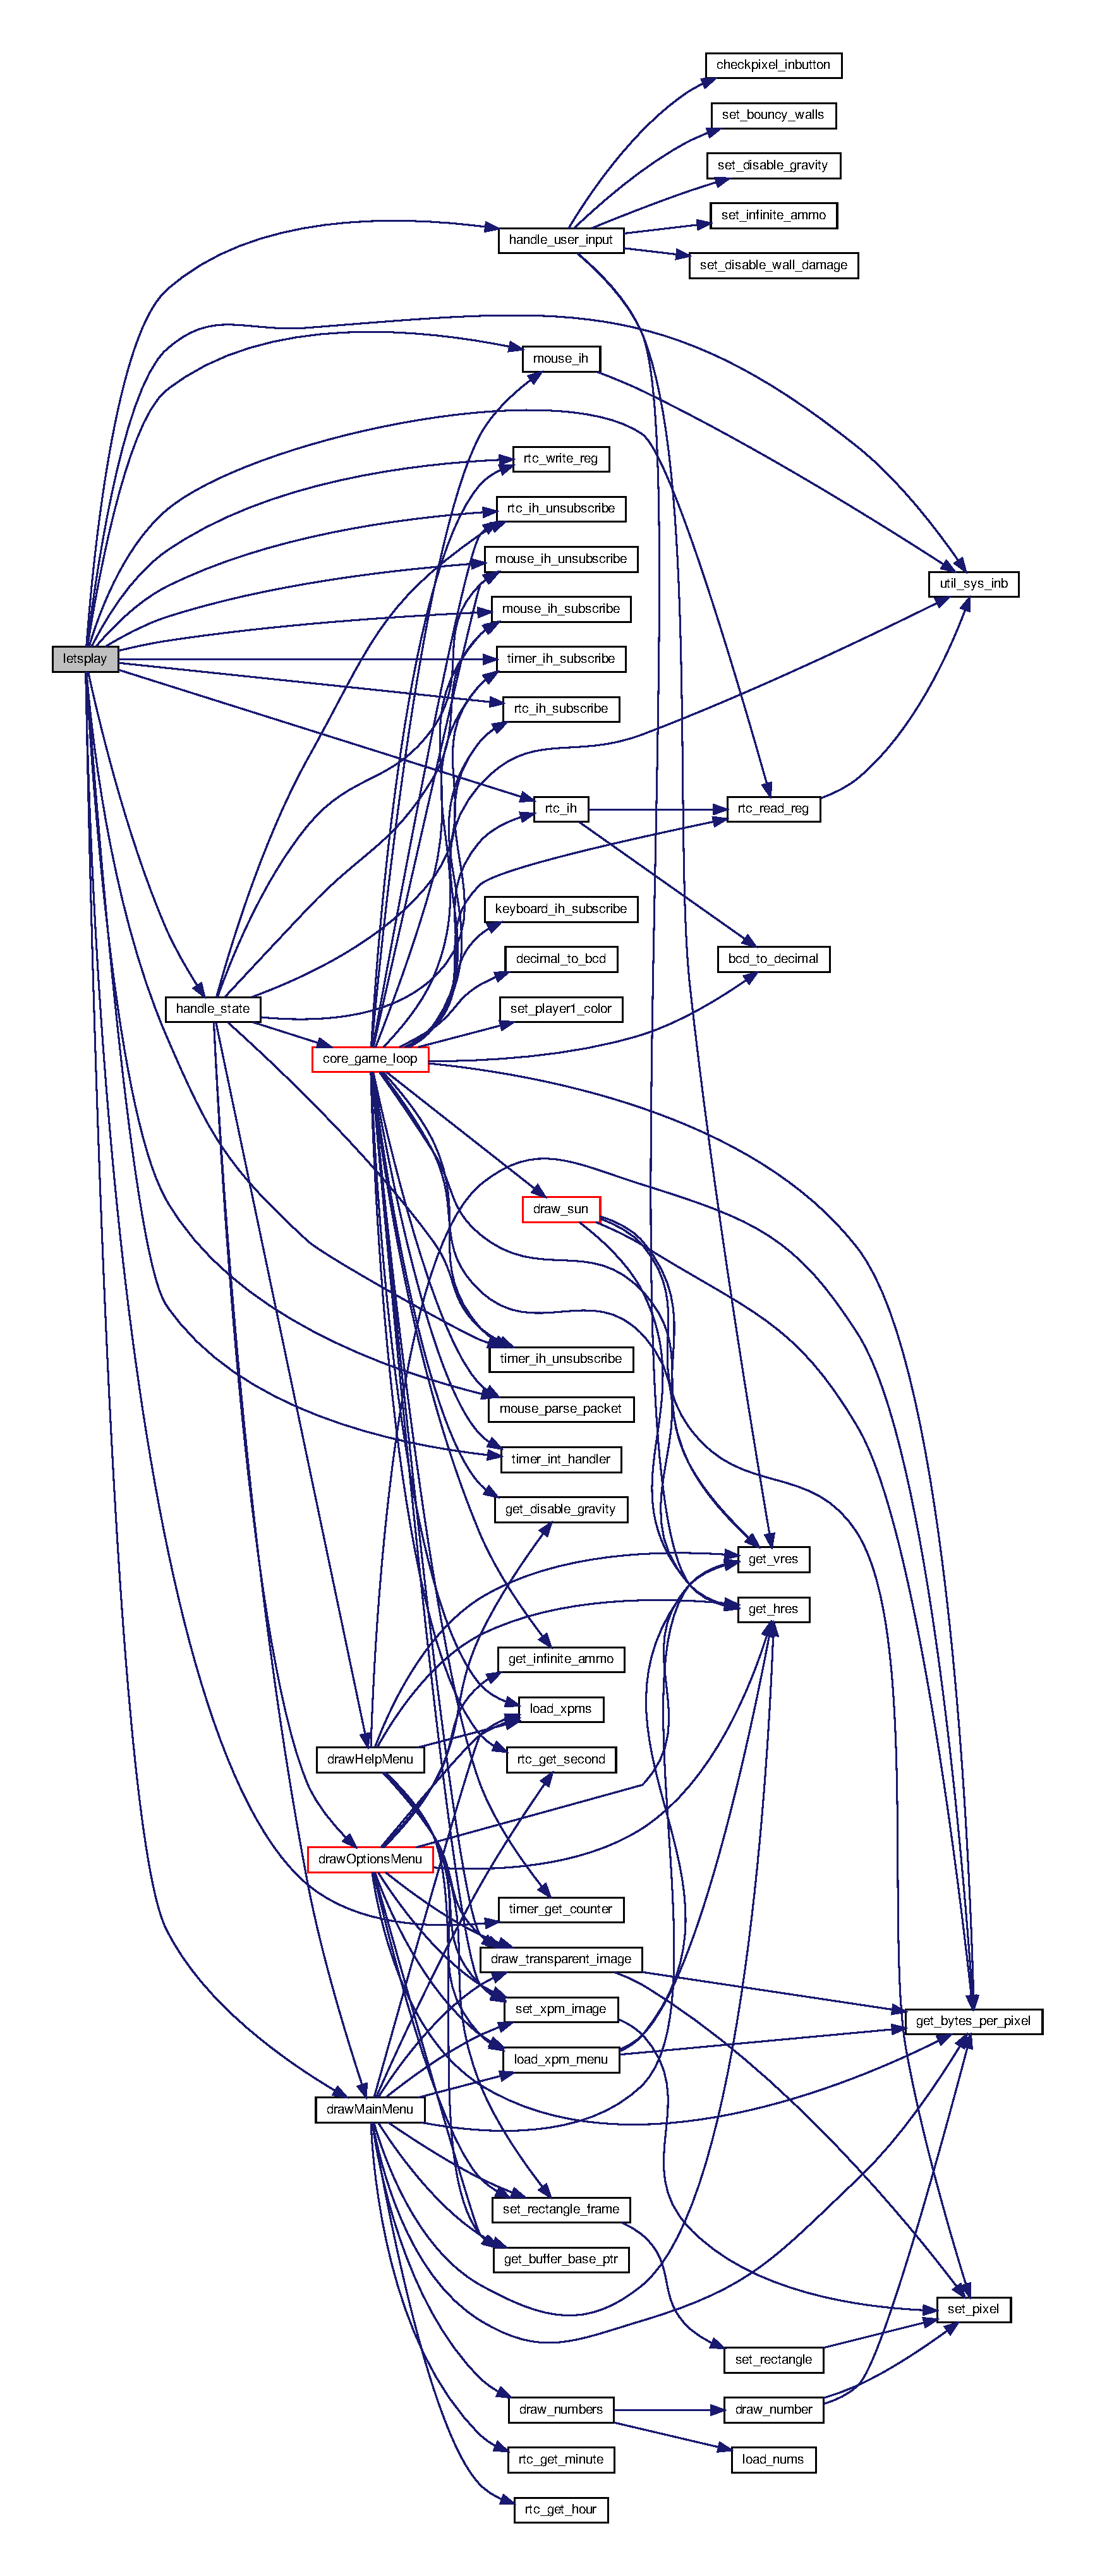
\includegraphics[height=550pt]{group__game_ga435b545b95a32afd525f8a1f05b2652c_cgraph}
\end{center}
\end{figure}

\hypertarget{group__gravity}{}\section{gravity}
\label{group__gravity}\index{gravity@{gravity}}


Gravity-\/related functions.  


\subsection*{Data Structures}
\begin{DoxyCompactItemize}
\item 
struct \hyperlink{structgravity__object}{gravity\+\_\+object}
\begin{DoxyCompactList}\small\item\em Struct that contains the position and velocity of an object. \end{DoxyCompactList}\end{DoxyCompactItemize}
\subsection*{Typedefs}
\begin{DoxyCompactItemize}
\item 
typedef struct \hyperlink{structgravity__object}{gravity\+\_\+object} \hyperlink{group__gravity_ga5aec6ca0c05d29e1a2708c89b0f27228}{gravity\+\_\+object}
\begin{DoxyCompactList}\small\item\em Struct that contains the position and velocity of an object. \end{DoxyCompactList}\end{DoxyCompactItemize}
\subsection*{Functions}
\begin{DoxyCompactItemize}
\item 
\hyperlink{structvector2}{vector2} \hyperlink{group__gravity_gadecebe4cd578161d35b325249079f7b9}{gravity\+\_\+acc\+\_\+vector} (\hyperlink{structvector2}{vector2} body\+\_\+pos, float body\+\_\+grav\+\_\+parameter, const \hyperlink{structgravity__object}{gravity\+\_\+object} $\ast$obj)
\begin{DoxyCompactList}\small\item\em Calculates the gravitational pull of a given body on \hyperlink{structgravity__object}{gravity\+\_\+object} obj. \end{DoxyCompactList}\item 
void \hyperlink{group__gravity_ga2cf5adbf1029afdd7b7cdd00eadc8771}{update\+\_\+gravity\+\_\+object} (\hyperlink{structgravity__object}{gravity\+\_\+object} $\ast$obj, \hyperlink{structvector2}{vector2} acc, float delta)
\begin{DoxyCompactList}\small\item\em Updates the velocity and position of obj, using something similar to the \href{https://en.wikipedia.org/wiki/Euler_method}{\tt Euler method} \end{DoxyCompactList}\end{DoxyCompactItemize}


\subsection{Detailed Description}
Gravity-\/related functions. 



\subsection{Typedef Documentation}
\mbox{\Hypertarget{group__gravity_ga5aec6ca0c05d29e1a2708c89b0f27228}\label{group__gravity_ga5aec6ca0c05d29e1a2708c89b0f27228}} 
\index{gravity@{gravity}!gravity\+\_\+object@{gravity\+\_\+object}}
\index{gravity\+\_\+object@{gravity\+\_\+object}!gravity@{gravity}}
\subsubsection{\texorpdfstring{gravity\+\_\+object}{gravity\_object}}
{\footnotesize\ttfamily typedef struct \hyperlink{structgravity__object}{gravity\+\_\+object}  \hyperlink{structgravity__object}{gravity\+\_\+object}}



Struct that contains the position and velocity of an object. 



\subsection{Function Documentation}
\mbox{\Hypertarget{group__gravity_gadecebe4cd578161d35b325249079f7b9}\label{group__gravity_gadecebe4cd578161d35b325249079f7b9}} 
\index{gravity@{gravity}!gravity\+\_\+acc\+\_\+vector@{gravity\+\_\+acc\+\_\+vector}}
\index{gravity\+\_\+acc\+\_\+vector@{gravity\+\_\+acc\+\_\+vector}!gravity@{gravity}}
\subsubsection{\texorpdfstring{gravity\+\_\+acc\+\_\+vector()}{gravity\_acc\_vector()}}
{\footnotesize\ttfamily \hyperlink{structvector2}{vector2} gravity\+\_\+acc\+\_\+vector (\begin{DoxyParamCaption}\item[{\hyperlink{structvector2}{vector2}}]{body\+\_\+pos,  }\item[{float}]{body\+\_\+grav\+\_\+parameter,  }\item[{const \hyperlink{structgravity__object}{gravity\+\_\+object} $\ast$}]{obj }\end{DoxyParamCaption})}



Calculates the gravitational pull of a given body on \hyperlink{structgravity__object}{gravity\+\_\+object} obj. 


\begin{DoxyParams}{Parameters}
{\em body\+\_\+pos} & The position of our body \\
\hline
{\em body\+\_\+grav\+\_\+parameter} & The \href{https://en.wikipedia.org/wiki/Standard_gravitational_parameter}{\tt gravitational parameter} of the body \\
\hline
{\em obj} & A pointer to the object whose gravitational acceleration will be calculated \\
\hline
\end{DoxyParams}
\begin{DoxyReturn}{Returns}
The gravitational acceleration vector of obj 
\end{DoxyReturn}
Here is the call graph for this function\+:\nopagebreak
\begin{figure}[H]
\begin{center}
\leavevmode
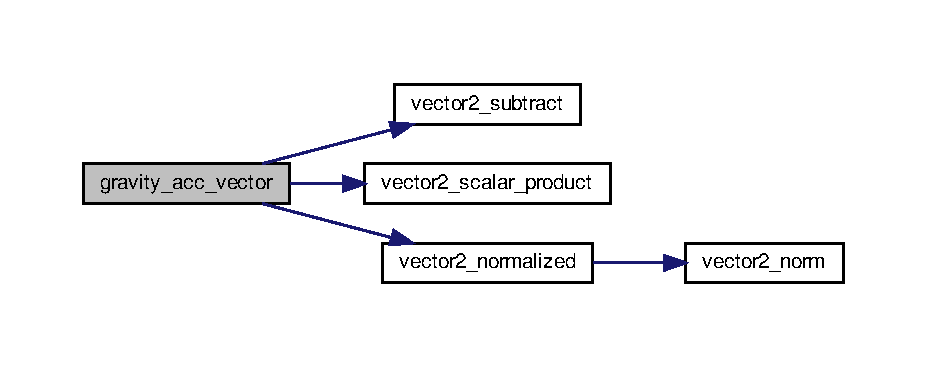
\includegraphics[width=350pt]{group__gravity_gadecebe4cd578161d35b325249079f7b9_cgraph}
\end{center}
\end{figure}
\mbox{\Hypertarget{group__gravity_ga2cf5adbf1029afdd7b7cdd00eadc8771}\label{group__gravity_ga2cf5adbf1029afdd7b7cdd00eadc8771}} 
\index{gravity@{gravity}!update\+\_\+gravity\+\_\+object@{update\+\_\+gravity\+\_\+object}}
\index{update\+\_\+gravity\+\_\+object@{update\+\_\+gravity\+\_\+object}!gravity@{gravity}}
\subsubsection{\texorpdfstring{update\+\_\+gravity\+\_\+object()}{update\_gravity\_object()}}
{\footnotesize\ttfamily void update\+\_\+gravity\+\_\+object (\begin{DoxyParamCaption}\item[{\hyperlink{structgravity__object}{gravity\+\_\+object} $\ast$}]{obj,  }\item[{\hyperlink{structvector2}{vector2}}]{acc,  }\item[{float}]{delta }\end{DoxyParamCaption})}



Updates the velocity and position of obj, using something similar to the \href{https://en.wikipedia.org/wiki/Euler_method}{\tt Euler method} 


\begin{DoxyParams}{Parameters}
{\em obj} & A pointer to the object whose state will be updated \\
\hline
{\em acc} & The acceleration that obj is subjected to \\
\hline
{\em delta} & The time delta in seconds \\
\hline
\end{DoxyParams}
Here is the call graph for this function\+:\nopagebreak
\begin{figure}[H]
\begin{center}
\leavevmode
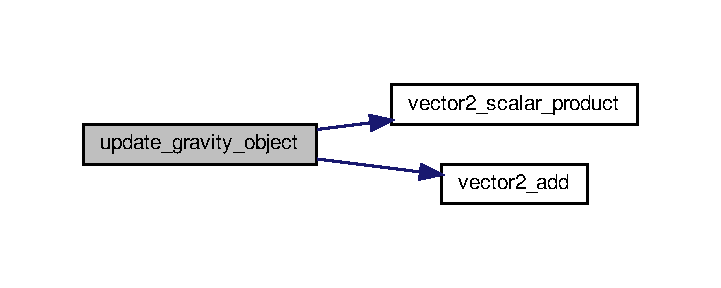
\includegraphics[width=346pt]{group__gravity_ga2cf5adbf1029afdd7b7cdd00eadc8771_cgraph}
\end{center}
\end{figure}

\hypertarget{group__kbc}{}\section{kbc}
\label{group__kbc}\index{kbc@{kbc}}


Functions related to the keyboard and mouse controller.  


\subsection*{Macros}
\begin{DoxyCompactItemize}
\item 
\#define \hyperlink{group__kbc_gab414f096b1781939124cd2ff672edb59}{K\+B\+C\+\_\+\+T\+I\+C\+K\+\_\+\+D\+E\+L\+AY}~20000
\item 
\#define \hyperlink{group__kbc_ga82a39176e42fe8f48025521b9674cdc6}{K\+B\+C\+\_\+\+P\+A\+R\+I\+TY}~B\+IT(7)
\item 
\#define \hyperlink{group__kbc_ga34599ca5c55cb9be3b235d7422aff45c}{K\+B\+C\+\_\+\+T\+I\+M\+E\+O\+UT}~B\+IT(6)
\item 
\#define \hyperlink{group__kbc_gaaa796d09d1e94025da456738295342f2}{K\+B\+C\+\_\+\+A\+UX}~B\+IT(5)
\item 
\#define \hyperlink{group__kbc_ga869c99dd1e3e026e766b3a1c75729df1}{K\+B\+C\+\_\+\+I\+NH}~B\+IT(4)
\item 
\#define \hyperlink{group__kbc_ga933a8846def486d800a725dc3959a74b}{K\+B\+C\+\_\+\+A2}~B\+IT(3)
\item 
\#define \hyperlink{group__kbc_ga9e3fddced5da8ee918cc20e74ff124d8}{K\+B\+C\+\_\+\+S\+YS}~B\+IT(2)
\item 
\#define \hyperlink{group__kbc_gac1649d41f8ba9a02fa70ec4e600d5e4a}{K\+B\+C\+\_\+\+I\+BF}~B\+IT(1)
\item 
\#define \hyperlink{group__kbc_ga36930de8a703505c95fe133095dcfe06}{K\+B\+C\+\_\+\+O\+BF}~B\+IT(0)
\item 
\#define \hyperlink{group__kbc_ga34b14687d83496940a236351fbbb1aea}{K\+B\+C\+\_\+\+S\+T\+A\+T\+\_\+\+R\+EG}~0x64
\item 
\#define \hyperlink{group__kbc_ga693314276867029f4c094442a261159f}{K\+B\+C\+\_\+\+C\+O\+M\+\_\+\+R\+EG}~0x64
\item 
\#define \hyperlink{group__kbc_ga1ccde68b2b6d4e45b50eef1403e10bb7}{K\+B\+C\+\_\+\+O\+U\+T\+\_\+\+B\+UF}~0x60
\item 
\#define \hyperlink{group__kbc_ga44b2468c0ea248ca480a8863b3f78c34}{K\+B\+C\+\_\+\+C\+O\+M\+\_\+\+A\+R\+G\+\_\+\+R\+EG}~0x60
\item 
\#define \hyperlink{group__kbc_ga67a2de56fabfdf65bfa20c50f8b77422}{K\+B\+C\+\_\+\+R\+E\+A\+D\+\_\+\+C\+OM}~0x20
\item 
\#define \hyperlink{group__kbc_ga09cb7b27cd3f4d0408f453da78ca294e}{K\+B\+C\+\_\+\+W\+R\+I\+T\+E\+\_\+\+C\+OM}~0x60
\item 
\#define \hyperlink{group__kbc_ga3add1395817336a078643ed6e0175ad6}{K\+B\+C\+\_\+\+S\+E\+L\+F\+\_\+\+T\+E\+ST}~0x\+AA
\item 
\#define \hyperlink{group__kbc_gab389a48497ca01296ca29c83c8eab2cd}{K\+B\+C\+\_\+\+C\+H\+E\+C\+K\+\_\+\+K\+B\+\_\+\+I\+N\+T\+E\+R\+F\+A\+CE}~0x\+AB
\item 
\#define \hyperlink{group__kbc_ga80e8aea5305350df2cc8811712caa6cc}{K\+B\+C\+\_\+\+D\+I\+S\+A\+B\+L\+E\+\_\+\+K\+B\+D\+\_\+\+I\+N\+T\+E\+R\+F\+A\+CE}~0x\+AD
\item 
\#define \hyperlink{group__kbc_ga728cbb4bd95a78097c116e7d4ce099a8}{K\+B\+C\+\_\+\+E\+N\+A\+B\+L\+E\+\_\+\+K\+B\+D\+\_\+\+I\+N\+T\+E\+R\+F\+A\+CE}~0x\+AE
\item 
\#define \hyperlink{group__kbc_ga1feec59f57ba28933fbe3516f30b1d14}{K\+B\+C\+\_\+\+D\+I\+S\+A\+B\+L\+E\+\_\+\+M\+O\+U\+SE}~0x\+A7
\item 
\#define \hyperlink{group__kbc_ga2c0f7ed5ff3b86d06f0e95600a5f736f}{K\+B\+C\+\_\+\+E\+N\+A\+B\+L\+E\+\_\+\+M\+O\+U\+SE}~0x\+A8
\item 
\#define \hyperlink{group__kbc_ga19f3f409be0e3cfa750c56408ef50f92}{K\+B\+C\+\_\+\+C\+H\+E\+C\+K\+\_\+\+M\+O\+U\+S\+E\+\_\+\+I\+N\+T\+E\+R\+F\+A\+CE}~0x\+A9
\item 
\#define \hyperlink{group__kbc_ga27c4267800118ec8c413f75f0bc45dc3}{K\+B\+C\+\_\+\+W\+R\+I\+T\+E\+\_\+\+B\+Y\+T\+E\+\_\+\+T\+O\+\_\+\+M\+O\+U\+SE}~0\+X\+D4
\item 
\#define \hyperlink{group__kbc_ga474cbc1b6540f557c0440d718b288ddd}{K\+B\+C\+\_\+\+C\+O\+M\+\_\+\+B\+Y\+T\+E\+\_\+\+D\+I\+S2}~B\+IT(5)
\item 
\#define \hyperlink{group__kbc_ga698b737cbe2182ee299347f00bc55ac1}{K\+B\+C\+\_\+\+C\+O\+M\+\_\+\+B\+Y\+T\+E\+\_\+\+D\+IS}~B\+IT(4)
\item 
\#define \hyperlink{group__kbc_ga35fe39f07554845d7c27a0b8d775cf25}{K\+B\+C\+\_\+\+C\+O\+M\+\_\+\+B\+Y\+T\+E\+\_\+\+I\+N\+T2}~B\+IT(1)
\item 
\#define \hyperlink{group__kbc_ga0574cae4394dc24a596d50361f31a1b3}{K\+B\+C\+\_\+\+C\+O\+M\+\_\+\+B\+Y\+T\+E\+\_\+\+I\+NT}~B\+IT(0)
\end{DoxyCompactItemize}
\subsection*{Functions}
\begin{DoxyCompactItemize}
\item 
void \hyperlink{group__kbc_ga594c74b8ef8c0d8a660bcdb729b1f381}{kbc\+\_\+delay} (int delay)
\begin{DoxyCompactList}\small\item\em Blocks the program by delay microseconds. \end{DoxyCompactList}\item 
int \hyperlink{group__kbc_ga8c467e640bc33719fe3ed7bcb73f2121}{kbc\+\_\+write\+\_\+command} (uint8\+\_\+t command)
\begin{DoxyCompactList}\small\item\em Sends a command to the kbc. \end{DoxyCompactList}\item 
int \hyperlink{group__kbc_ga24f1a4d1bcb60a73ebd6cee462191a52}{kbc\+\_\+write\+\_\+command\+\_\+arg} (uint8\+\_\+t arg)
\begin{DoxyCompactList}\small\item\em Sends an argument to the kbc. \end{DoxyCompactList}\item 
int \hyperlink{group__kbc_ga65f11cca39a73154ab68dabac8b12683}{kbc\+\_\+read\+\_\+command\+\_\+result} (uint8\+\_\+t $\ast$result)
\begin{DoxyCompactList}\small\item\em Reads a command result from the kbc. \end{DoxyCompactList}\item 
int \hyperlink{group__kbc_gadc6d5fbf9c3a43d168962776591ac75b}{kbc\+\_\+read\+\_\+command\+\_\+byte} (uint8\+\_\+t $\ast$command\+\_\+byte)
\begin{DoxyCompactList}\small\item\em Reads the command byte from the kbc. \end{DoxyCompactList}\item 
int \hyperlink{group__kbc_ga5e840dccbbe5abccff8ca66f78c476c9}{kbc\+\_\+write\+\_\+command\+\_\+byte} (uint8\+\_\+t command\+\_\+byte)
\begin{DoxyCompactList}\small\item\em Sends a command byte to the kbc. \end{DoxyCompactList}\item 
int \hyperlink{group__kbc_gaa4c58a11cd49c54cc0eb02a79010a9cc}{kbc\+\_\+read\+\_\+status} (uint8\+\_\+t $\ast$status)
\begin{DoxyCompactList}\small\item\em Reads the status of the kbc. \end{DoxyCompactList}\end{DoxyCompactItemize}


\subsection{Detailed Description}
Functions related to the keyboard and mouse controller. 



\subsection{Macro Definition Documentation}
\mbox{\Hypertarget{group__kbc_ga933a8846def486d800a725dc3959a74b}\label{group__kbc_ga933a8846def486d800a725dc3959a74b}} 
\index{kbc@{kbc}!K\+B\+C\+\_\+\+A2@{K\+B\+C\+\_\+\+A2}}
\index{K\+B\+C\+\_\+\+A2@{K\+B\+C\+\_\+\+A2}!kbc@{kbc}}
\subsubsection{\texorpdfstring{K\+B\+C\+\_\+\+A2}{KBC\_A2}}
{\footnotesize\ttfamily \#define K\+B\+C\+\_\+\+A2~B\+IT(3)}

\mbox{\Hypertarget{group__kbc_gaaa796d09d1e94025da456738295342f2}\label{group__kbc_gaaa796d09d1e94025da456738295342f2}} 
\index{kbc@{kbc}!K\+B\+C\+\_\+\+A\+UX@{K\+B\+C\+\_\+\+A\+UX}}
\index{K\+B\+C\+\_\+\+A\+UX@{K\+B\+C\+\_\+\+A\+UX}!kbc@{kbc}}
\subsubsection{\texorpdfstring{K\+B\+C\+\_\+\+A\+UX}{KBC\_AUX}}
{\footnotesize\ttfamily \#define K\+B\+C\+\_\+\+A\+UX~B\+IT(5)}

\mbox{\Hypertarget{group__kbc_gab389a48497ca01296ca29c83c8eab2cd}\label{group__kbc_gab389a48497ca01296ca29c83c8eab2cd}} 
\index{kbc@{kbc}!K\+B\+C\+\_\+\+C\+H\+E\+C\+K\+\_\+\+K\+B\+\_\+\+I\+N\+T\+E\+R\+F\+A\+CE@{K\+B\+C\+\_\+\+C\+H\+E\+C\+K\+\_\+\+K\+B\+\_\+\+I\+N\+T\+E\+R\+F\+A\+CE}}
\index{K\+B\+C\+\_\+\+C\+H\+E\+C\+K\+\_\+\+K\+B\+\_\+\+I\+N\+T\+E\+R\+F\+A\+CE@{K\+B\+C\+\_\+\+C\+H\+E\+C\+K\+\_\+\+K\+B\+\_\+\+I\+N\+T\+E\+R\+F\+A\+CE}!kbc@{kbc}}
\subsubsection{\texorpdfstring{K\+B\+C\+\_\+\+C\+H\+E\+C\+K\+\_\+\+K\+B\+\_\+\+I\+N\+T\+E\+R\+F\+A\+CE}{KBC\_CHECK\_KB\_INTERFACE}}
{\footnotesize\ttfamily \#define K\+B\+C\+\_\+\+C\+H\+E\+C\+K\+\_\+\+K\+B\+\_\+\+I\+N\+T\+E\+R\+F\+A\+CE~0x\+AB}

\mbox{\Hypertarget{group__kbc_ga19f3f409be0e3cfa750c56408ef50f92}\label{group__kbc_ga19f3f409be0e3cfa750c56408ef50f92}} 
\index{kbc@{kbc}!K\+B\+C\+\_\+\+C\+H\+E\+C\+K\+\_\+\+M\+O\+U\+S\+E\+\_\+\+I\+N\+T\+E\+R\+F\+A\+CE@{K\+B\+C\+\_\+\+C\+H\+E\+C\+K\+\_\+\+M\+O\+U\+S\+E\+\_\+\+I\+N\+T\+E\+R\+F\+A\+CE}}
\index{K\+B\+C\+\_\+\+C\+H\+E\+C\+K\+\_\+\+M\+O\+U\+S\+E\+\_\+\+I\+N\+T\+E\+R\+F\+A\+CE@{K\+B\+C\+\_\+\+C\+H\+E\+C\+K\+\_\+\+M\+O\+U\+S\+E\+\_\+\+I\+N\+T\+E\+R\+F\+A\+CE}!kbc@{kbc}}
\subsubsection{\texorpdfstring{K\+B\+C\+\_\+\+C\+H\+E\+C\+K\+\_\+\+M\+O\+U\+S\+E\+\_\+\+I\+N\+T\+E\+R\+F\+A\+CE}{KBC\_CHECK\_MOUSE\_INTERFACE}}
{\footnotesize\ttfamily \#define K\+B\+C\+\_\+\+C\+H\+E\+C\+K\+\_\+\+M\+O\+U\+S\+E\+\_\+\+I\+N\+T\+E\+R\+F\+A\+CE~0x\+A9}

\mbox{\Hypertarget{group__kbc_ga44b2468c0ea248ca480a8863b3f78c34}\label{group__kbc_ga44b2468c0ea248ca480a8863b3f78c34}} 
\index{kbc@{kbc}!K\+B\+C\+\_\+\+C\+O\+M\+\_\+\+A\+R\+G\+\_\+\+R\+EG@{K\+B\+C\+\_\+\+C\+O\+M\+\_\+\+A\+R\+G\+\_\+\+R\+EG}}
\index{K\+B\+C\+\_\+\+C\+O\+M\+\_\+\+A\+R\+G\+\_\+\+R\+EG@{K\+B\+C\+\_\+\+C\+O\+M\+\_\+\+A\+R\+G\+\_\+\+R\+EG}!kbc@{kbc}}
\subsubsection{\texorpdfstring{K\+B\+C\+\_\+\+C\+O\+M\+\_\+\+A\+R\+G\+\_\+\+R\+EG}{KBC\_COM\_ARG\_REG}}
{\footnotesize\ttfamily \#define K\+B\+C\+\_\+\+C\+O\+M\+\_\+\+A\+R\+G\+\_\+\+R\+EG~0x60}

\mbox{\Hypertarget{group__kbc_ga698b737cbe2182ee299347f00bc55ac1}\label{group__kbc_ga698b737cbe2182ee299347f00bc55ac1}} 
\index{kbc@{kbc}!K\+B\+C\+\_\+\+C\+O\+M\+\_\+\+B\+Y\+T\+E\+\_\+\+D\+IS@{K\+B\+C\+\_\+\+C\+O\+M\+\_\+\+B\+Y\+T\+E\+\_\+\+D\+IS}}
\index{K\+B\+C\+\_\+\+C\+O\+M\+\_\+\+B\+Y\+T\+E\+\_\+\+D\+IS@{K\+B\+C\+\_\+\+C\+O\+M\+\_\+\+B\+Y\+T\+E\+\_\+\+D\+IS}!kbc@{kbc}}
\subsubsection{\texorpdfstring{K\+B\+C\+\_\+\+C\+O\+M\+\_\+\+B\+Y\+T\+E\+\_\+\+D\+IS}{KBC\_COM\_BYTE\_DIS}}
{\footnotesize\ttfamily \#define K\+B\+C\+\_\+\+C\+O\+M\+\_\+\+B\+Y\+T\+E\+\_\+\+D\+IS~B\+IT(4)}

\mbox{\Hypertarget{group__kbc_ga474cbc1b6540f557c0440d718b288ddd}\label{group__kbc_ga474cbc1b6540f557c0440d718b288ddd}} 
\index{kbc@{kbc}!K\+B\+C\+\_\+\+C\+O\+M\+\_\+\+B\+Y\+T\+E\+\_\+\+D\+I\+S2@{K\+B\+C\+\_\+\+C\+O\+M\+\_\+\+B\+Y\+T\+E\+\_\+\+D\+I\+S2}}
\index{K\+B\+C\+\_\+\+C\+O\+M\+\_\+\+B\+Y\+T\+E\+\_\+\+D\+I\+S2@{K\+B\+C\+\_\+\+C\+O\+M\+\_\+\+B\+Y\+T\+E\+\_\+\+D\+I\+S2}!kbc@{kbc}}
\subsubsection{\texorpdfstring{K\+B\+C\+\_\+\+C\+O\+M\+\_\+\+B\+Y\+T\+E\+\_\+\+D\+I\+S2}{KBC\_COM\_BYTE\_DIS2}}
{\footnotesize\ttfamily \#define K\+B\+C\+\_\+\+C\+O\+M\+\_\+\+B\+Y\+T\+E\+\_\+\+D\+I\+S2~B\+IT(5)}

\mbox{\Hypertarget{group__kbc_ga0574cae4394dc24a596d50361f31a1b3}\label{group__kbc_ga0574cae4394dc24a596d50361f31a1b3}} 
\index{kbc@{kbc}!K\+B\+C\+\_\+\+C\+O\+M\+\_\+\+B\+Y\+T\+E\+\_\+\+I\+NT@{K\+B\+C\+\_\+\+C\+O\+M\+\_\+\+B\+Y\+T\+E\+\_\+\+I\+NT}}
\index{K\+B\+C\+\_\+\+C\+O\+M\+\_\+\+B\+Y\+T\+E\+\_\+\+I\+NT@{K\+B\+C\+\_\+\+C\+O\+M\+\_\+\+B\+Y\+T\+E\+\_\+\+I\+NT}!kbc@{kbc}}
\subsubsection{\texorpdfstring{K\+B\+C\+\_\+\+C\+O\+M\+\_\+\+B\+Y\+T\+E\+\_\+\+I\+NT}{KBC\_COM\_BYTE\_INT}}
{\footnotesize\ttfamily \#define K\+B\+C\+\_\+\+C\+O\+M\+\_\+\+B\+Y\+T\+E\+\_\+\+I\+NT~B\+IT(0)}

\mbox{\Hypertarget{group__kbc_ga35fe39f07554845d7c27a0b8d775cf25}\label{group__kbc_ga35fe39f07554845d7c27a0b8d775cf25}} 
\index{kbc@{kbc}!K\+B\+C\+\_\+\+C\+O\+M\+\_\+\+B\+Y\+T\+E\+\_\+\+I\+N\+T2@{K\+B\+C\+\_\+\+C\+O\+M\+\_\+\+B\+Y\+T\+E\+\_\+\+I\+N\+T2}}
\index{K\+B\+C\+\_\+\+C\+O\+M\+\_\+\+B\+Y\+T\+E\+\_\+\+I\+N\+T2@{K\+B\+C\+\_\+\+C\+O\+M\+\_\+\+B\+Y\+T\+E\+\_\+\+I\+N\+T2}!kbc@{kbc}}
\subsubsection{\texorpdfstring{K\+B\+C\+\_\+\+C\+O\+M\+\_\+\+B\+Y\+T\+E\+\_\+\+I\+N\+T2}{KBC\_COM\_BYTE\_INT2}}
{\footnotesize\ttfamily \#define K\+B\+C\+\_\+\+C\+O\+M\+\_\+\+B\+Y\+T\+E\+\_\+\+I\+N\+T2~B\+IT(1)}

\mbox{\Hypertarget{group__kbc_ga693314276867029f4c094442a261159f}\label{group__kbc_ga693314276867029f4c094442a261159f}} 
\index{kbc@{kbc}!K\+B\+C\+\_\+\+C\+O\+M\+\_\+\+R\+EG@{K\+B\+C\+\_\+\+C\+O\+M\+\_\+\+R\+EG}}
\index{K\+B\+C\+\_\+\+C\+O\+M\+\_\+\+R\+EG@{K\+B\+C\+\_\+\+C\+O\+M\+\_\+\+R\+EG}!kbc@{kbc}}
\subsubsection{\texorpdfstring{K\+B\+C\+\_\+\+C\+O\+M\+\_\+\+R\+EG}{KBC\_COM\_REG}}
{\footnotesize\ttfamily \#define K\+B\+C\+\_\+\+C\+O\+M\+\_\+\+R\+EG~0x64}

\mbox{\Hypertarget{group__kbc_ga80e8aea5305350df2cc8811712caa6cc}\label{group__kbc_ga80e8aea5305350df2cc8811712caa6cc}} 
\index{kbc@{kbc}!K\+B\+C\+\_\+\+D\+I\+S\+A\+B\+L\+E\+\_\+\+K\+B\+D\+\_\+\+I\+N\+T\+E\+R\+F\+A\+CE@{K\+B\+C\+\_\+\+D\+I\+S\+A\+B\+L\+E\+\_\+\+K\+B\+D\+\_\+\+I\+N\+T\+E\+R\+F\+A\+CE}}
\index{K\+B\+C\+\_\+\+D\+I\+S\+A\+B\+L\+E\+\_\+\+K\+B\+D\+\_\+\+I\+N\+T\+E\+R\+F\+A\+CE@{K\+B\+C\+\_\+\+D\+I\+S\+A\+B\+L\+E\+\_\+\+K\+B\+D\+\_\+\+I\+N\+T\+E\+R\+F\+A\+CE}!kbc@{kbc}}
\subsubsection{\texorpdfstring{K\+B\+C\+\_\+\+D\+I\+S\+A\+B\+L\+E\+\_\+\+K\+B\+D\+\_\+\+I\+N\+T\+E\+R\+F\+A\+CE}{KBC\_DISABLE\_KBD\_INTERFACE}}
{\footnotesize\ttfamily \#define K\+B\+C\+\_\+\+D\+I\+S\+A\+B\+L\+E\+\_\+\+K\+B\+D\+\_\+\+I\+N\+T\+E\+R\+F\+A\+CE~0x\+AD}

\mbox{\Hypertarget{group__kbc_ga1feec59f57ba28933fbe3516f30b1d14}\label{group__kbc_ga1feec59f57ba28933fbe3516f30b1d14}} 
\index{kbc@{kbc}!K\+B\+C\+\_\+\+D\+I\+S\+A\+B\+L\+E\+\_\+\+M\+O\+U\+SE@{K\+B\+C\+\_\+\+D\+I\+S\+A\+B\+L\+E\+\_\+\+M\+O\+U\+SE}}
\index{K\+B\+C\+\_\+\+D\+I\+S\+A\+B\+L\+E\+\_\+\+M\+O\+U\+SE@{K\+B\+C\+\_\+\+D\+I\+S\+A\+B\+L\+E\+\_\+\+M\+O\+U\+SE}!kbc@{kbc}}
\subsubsection{\texorpdfstring{K\+B\+C\+\_\+\+D\+I\+S\+A\+B\+L\+E\+\_\+\+M\+O\+U\+SE}{KBC\_DISABLE\_MOUSE}}
{\footnotesize\ttfamily \#define K\+B\+C\+\_\+\+D\+I\+S\+A\+B\+L\+E\+\_\+\+M\+O\+U\+SE~0x\+A7}

\mbox{\Hypertarget{group__kbc_ga728cbb4bd95a78097c116e7d4ce099a8}\label{group__kbc_ga728cbb4bd95a78097c116e7d4ce099a8}} 
\index{kbc@{kbc}!K\+B\+C\+\_\+\+E\+N\+A\+B\+L\+E\+\_\+\+K\+B\+D\+\_\+\+I\+N\+T\+E\+R\+F\+A\+CE@{K\+B\+C\+\_\+\+E\+N\+A\+B\+L\+E\+\_\+\+K\+B\+D\+\_\+\+I\+N\+T\+E\+R\+F\+A\+CE}}
\index{K\+B\+C\+\_\+\+E\+N\+A\+B\+L\+E\+\_\+\+K\+B\+D\+\_\+\+I\+N\+T\+E\+R\+F\+A\+CE@{K\+B\+C\+\_\+\+E\+N\+A\+B\+L\+E\+\_\+\+K\+B\+D\+\_\+\+I\+N\+T\+E\+R\+F\+A\+CE}!kbc@{kbc}}
\subsubsection{\texorpdfstring{K\+B\+C\+\_\+\+E\+N\+A\+B\+L\+E\+\_\+\+K\+B\+D\+\_\+\+I\+N\+T\+E\+R\+F\+A\+CE}{KBC\_ENABLE\_KBD\_INTERFACE}}
{\footnotesize\ttfamily \#define K\+B\+C\+\_\+\+E\+N\+A\+B\+L\+E\+\_\+\+K\+B\+D\+\_\+\+I\+N\+T\+E\+R\+F\+A\+CE~0x\+AE}

\mbox{\Hypertarget{group__kbc_ga2c0f7ed5ff3b86d06f0e95600a5f736f}\label{group__kbc_ga2c0f7ed5ff3b86d06f0e95600a5f736f}} 
\index{kbc@{kbc}!K\+B\+C\+\_\+\+E\+N\+A\+B\+L\+E\+\_\+\+M\+O\+U\+SE@{K\+B\+C\+\_\+\+E\+N\+A\+B\+L\+E\+\_\+\+M\+O\+U\+SE}}
\index{K\+B\+C\+\_\+\+E\+N\+A\+B\+L\+E\+\_\+\+M\+O\+U\+SE@{K\+B\+C\+\_\+\+E\+N\+A\+B\+L\+E\+\_\+\+M\+O\+U\+SE}!kbc@{kbc}}
\subsubsection{\texorpdfstring{K\+B\+C\+\_\+\+E\+N\+A\+B\+L\+E\+\_\+\+M\+O\+U\+SE}{KBC\_ENABLE\_MOUSE}}
{\footnotesize\ttfamily \#define K\+B\+C\+\_\+\+E\+N\+A\+B\+L\+E\+\_\+\+M\+O\+U\+SE~0x\+A8}

\mbox{\Hypertarget{group__kbc_gac1649d41f8ba9a02fa70ec4e600d5e4a}\label{group__kbc_gac1649d41f8ba9a02fa70ec4e600d5e4a}} 
\index{kbc@{kbc}!K\+B\+C\+\_\+\+I\+BF@{K\+B\+C\+\_\+\+I\+BF}}
\index{K\+B\+C\+\_\+\+I\+BF@{K\+B\+C\+\_\+\+I\+BF}!kbc@{kbc}}
\subsubsection{\texorpdfstring{K\+B\+C\+\_\+\+I\+BF}{KBC\_IBF}}
{\footnotesize\ttfamily \#define K\+B\+C\+\_\+\+I\+BF~B\+IT(1)}

\mbox{\Hypertarget{group__kbc_ga869c99dd1e3e026e766b3a1c75729df1}\label{group__kbc_ga869c99dd1e3e026e766b3a1c75729df1}} 
\index{kbc@{kbc}!K\+B\+C\+\_\+\+I\+NH@{K\+B\+C\+\_\+\+I\+NH}}
\index{K\+B\+C\+\_\+\+I\+NH@{K\+B\+C\+\_\+\+I\+NH}!kbc@{kbc}}
\subsubsection{\texorpdfstring{K\+B\+C\+\_\+\+I\+NH}{KBC\_INH}}
{\footnotesize\ttfamily \#define K\+B\+C\+\_\+\+I\+NH~B\+IT(4)}

\mbox{\Hypertarget{group__kbc_ga36930de8a703505c95fe133095dcfe06}\label{group__kbc_ga36930de8a703505c95fe133095dcfe06}} 
\index{kbc@{kbc}!K\+B\+C\+\_\+\+O\+BF@{K\+B\+C\+\_\+\+O\+BF}}
\index{K\+B\+C\+\_\+\+O\+BF@{K\+B\+C\+\_\+\+O\+BF}!kbc@{kbc}}
\subsubsection{\texorpdfstring{K\+B\+C\+\_\+\+O\+BF}{KBC\_OBF}}
{\footnotesize\ttfamily \#define K\+B\+C\+\_\+\+O\+BF~B\+IT(0)}

\mbox{\Hypertarget{group__kbc_ga1ccde68b2b6d4e45b50eef1403e10bb7}\label{group__kbc_ga1ccde68b2b6d4e45b50eef1403e10bb7}} 
\index{kbc@{kbc}!K\+B\+C\+\_\+\+O\+U\+T\+\_\+\+B\+UF@{K\+B\+C\+\_\+\+O\+U\+T\+\_\+\+B\+UF}}
\index{K\+B\+C\+\_\+\+O\+U\+T\+\_\+\+B\+UF@{K\+B\+C\+\_\+\+O\+U\+T\+\_\+\+B\+UF}!kbc@{kbc}}
\subsubsection{\texorpdfstring{K\+B\+C\+\_\+\+O\+U\+T\+\_\+\+B\+UF}{KBC\_OUT\_BUF}}
{\footnotesize\ttfamily \#define K\+B\+C\+\_\+\+O\+U\+T\+\_\+\+B\+UF~0x60}

\mbox{\Hypertarget{group__kbc_ga82a39176e42fe8f48025521b9674cdc6}\label{group__kbc_ga82a39176e42fe8f48025521b9674cdc6}} 
\index{kbc@{kbc}!K\+B\+C\+\_\+\+P\+A\+R\+I\+TY@{K\+B\+C\+\_\+\+P\+A\+R\+I\+TY}}
\index{K\+B\+C\+\_\+\+P\+A\+R\+I\+TY@{K\+B\+C\+\_\+\+P\+A\+R\+I\+TY}!kbc@{kbc}}
\subsubsection{\texorpdfstring{K\+B\+C\+\_\+\+P\+A\+R\+I\+TY}{KBC\_PARITY}}
{\footnotesize\ttfamily \#define K\+B\+C\+\_\+\+P\+A\+R\+I\+TY~B\+IT(7)}

\mbox{\Hypertarget{group__kbc_ga67a2de56fabfdf65bfa20c50f8b77422}\label{group__kbc_ga67a2de56fabfdf65bfa20c50f8b77422}} 
\index{kbc@{kbc}!K\+B\+C\+\_\+\+R\+E\+A\+D\+\_\+\+C\+OM@{K\+B\+C\+\_\+\+R\+E\+A\+D\+\_\+\+C\+OM}}
\index{K\+B\+C\+\_\+\+R\+E\+A\+D\+\_\+\+C\+OM@{K\+B\+C\+\_\+\+R\+E\+A\+D\+\_\+\+C\+OM}!kbc@{kbc}}
\subsubsection{\texorpdfstring{K\+B\+C\+\_\+\+R\+E\+A\+D\+\_\+\+C\+OM}{KBC\_READ\_COM}}
{\footnotesize\ttfamily \#define K\+B\+C\+\_\+\+R\+E\+A\+D\+\_\+\+C\+OM~0x20}

\mbox{\Hypertarget{group__kbc_ga3add1395817336a078643ed6e0175ad6}\label{group__kbc_ga3add1395817336a078643ed6e0175ad6}} 
\index{kbc@{kbc}!K\+B\+C\+\_\+\+S\+E\+L\+F\+\_\+\+T\+E\+ST@{K\+B\+C\+\_\+\+S\+E\+L\+F\+\_\+\+T\+E\+ST}}
\index{K\+B\+C\+\_\+\+S\+E\+L\+F\+\_\+\+T\+E\+ST@{K\+B\+C\+\_\+\+S\+E\+L\+F\+\_\+\+T\+E\+ST}!kbc@{kbc}}
\subsubsection{\texorpdfstring{K\+B\+C\+\_\+\+S\+E\+L\+F\+\_\+\+T\+E\+ST}{KBC\_SELF\_TEST}}
{\footnotesize\ttfamily \#define K\+B\+C\+\_\+\+S\+E\+L\+F\+\_\+\+T\+E\+ST~0x\+AA}

\mbox{\Hypertarget{group__kbc_ga34b14687d83496940a236351fbbb1aea}\label{group__kbc_ga34b14687d83496940a236351fbbb1aea}} 
\index{kbc@{kbc}!K\+B\+C\+\_\+\+S\+T\+A\+T\+\_\+\+R\+EG@{K\+B\+C\+\_\+\+S\+T\+A\+T\+\_\+\+R\+EG}}
\index{K\+B\+C\+\_\+\+S\+T\+A\+T\+\_\+\+R\+EG@{K\+B\+C\+\_\+\+S\+T\+A\+T\+\_\+\+R\+EG}!kbc@{kbc}}
\subsubsection{\texorpdfstring{K\+B\+C\+\_\+\+S\+T\+A\+T\+\_\+\+R\+EG}{KBC\_STAT\_REG}}
{\footnotesize\ttfamily \#define K\+B\+C\+\_\+\+S\+T\+A\+T\+\_\+\+R\+EG~0x64}

\mbox{\Hypertarget{group__kbc_ga9e3fddced5da8ee918cc20e74ff124d8}\label{group__kbc_ga9e3fddced5da8ee918cc20e74ff124d8}} 
\index{kbc@{kbc}!K\+B\+C\+\_\+\+S\+YS@{K\+B\+C\+\_\+\+S\+YS}}
\index{K\+B\+C\+\_\+\+S\+YS@{K\+B\+C\+\_\+\+S\+YS}!kbc@{kbc}}
\subsubsection{\texorpdfstring{K\+B\+C\+\_\+\+S\+YS}{KBC\_SYS}}
{\footnotesize\ttfamily \#define K\+B\+C\+\_\+\+S\+YS~B\+IT(2)}

\mbox{\Hypertarget{group__kbc_gab414f096b1781939124cd2ff672edb59}\label{group__kbc_gab414f096b1781939124cd2ff672edb59}} 
\index{kbc@{kbc}!K\+B\+C\+\_\+\+T\+I\+C\+K\+\_\+\+D\+E\+L\+AY@{K\+B\+C\+\_\+\+T\+I\+C\+K\+\_\+\+D\+E\+L\+AY}}
\index{K\+B\+C\+\_\+\+T\+I\+C\+K\+\_\+\+D\+E\+L\+AY@{K\+B\+C\+\_\+\+T\+I\+C\+K\+\_\+\+D\+E\+L\+AY}!kbc@{kbc}}
\subsubsection{\texorpdfstring{K\+B\+C\+\_\+\+T\+I\+C\+K\+\_\+\+D\+E\+L\+AY}{KBC\_TICK\_DELAY}}
{\footnotesize\ttfamily \#define K\+B\+C\+\_\+\+T\+I\+C\+K\+\_\+\+D\+E\+L\+AY~20000}

\mbox{\Hypertarget{group__kbc_ga34599ca5c55cb9be3b235d7422aff45c}\label{group__kbc_ga34599ca5c55cb9be3b235d7422aff45c}} 
\index{kbc@{kbc}!K\+B\+C\+\_\+\+T\+I\+M\+E\+O\+UT@{K\+B\+C\+\_\+\+T\+I\+M\+E\+O\+UT}}
\index{K\+B\+C\+\_\+\+T\+I\+M\+E\+O\+UT@{K\+B\+C\+\_\+\+T\+I\+M\+E\+O\+UT}!kbc@{kbc}}
\subsubsection{\texorpdfstring{K\+B\+C\+\_\+\+T\+I\+M\+E\+O\+UT}{KBC\_TIMEOUT}}
{\footnotesize\ttfamily \#define K\+B\+C\+\_\+\+T\+I\+M\+E\+O\+UT~B\+IT(6)}

\mbox{\Hypertarget{group__kbc_ga27c4267800118ec8c413f75f0bc45dc3}\label{group__kbc_ga27c4267800118ec8c413f75f0bc45dc3}} 
\index{kbc@{kbc}!K\+B\+C\+\_\+\+W\+R\+I\+T\+E\+\_\+\+B\+Y\+T\+E\+\_\+\+T\+O\+\_\+\+M\+O\+U\+SE@{K\+B\+C\+\_\+\+W\+R\+I\+T\+E\+\_\+\+B\+Y\+T\+E\+\_\+\+T\+O\+\_\+\+M\+O\+U\+SE}}
\index{K\+B\+C\+\_\+\+W\+R\+I\+T\+E\+\_\+\+B\+Y\+T\+E\+\_\+\+T\+O\+\_\+\+M\+O\+U\+SE@{K\+B\+C\+\_\+\+W\+R\+I\+T\+E\+\_\+\+B\+Y\+T\+E\+\_\+\+T\+O\+\_\+\+M\+O\+U\+SE}!kbc@{kbc}}
\subsubsection{\texorpdfstring{K\+B\+C\+\_\+\+W\+R\+I\+T\+E\+\_\+\+B\+Y\+T\+E\+\_\+\+T\+O\+\_\+\+M\+O\+U\+SE}{KBC\_WRITE\_BYTE\_TO\_MOUSE}}
{\footnotesize\ttfamily \#define K\+B\+C\+\_\+\+W\+R\+I\+T\+E\+\_\+\+B\+Y\+T\+E\+\_\+\+T\+O\+\_\+\+M\+O\+U\+SE~0\+X\+D4}

\mbox{\Hypertarget{group__kbc_ga09cb7b27cd3f4d0408f453da78ca294e}\label{group__kbc_ga09cb7b27cd3f4d0408f453da78ca294e}} 
\index{kbc@{kbc}!K\+B\+C\+\_\+\+W\+R\+I\+T\+E\+\_\+\+C\+OM@{K\+B\+C\+\_\+\+W\+R\+I\+T\+E\+\_\+\+C\+OM}}
\index{K\+B\+C\+\_\+\+W\+R\+I\+T\+E\+\_\+\+C\+OM@{K\+B\+C\+\_\+\+W\+R\+I\+T\+E\+\_\+\+C\+OM}!kbc@{kbc}}
\subsubsection{\texorpdfstring{K\+B\+C\+\_\+\+W\+R\+I\+T\+E\+\_\+\+C\+OM}{KBC\_WRITE\_COM}}
{\footnotesize\ttfamily \#define K\+B\+C\+\_\+\+W\+R\+I\+T\+E\+\_\+\+C\+OM~0x60}



\subsection{Function Documentation}
\mbox{\Hypertarget{group__kbc_ga594c74b8ef8c0d8a660bcdb729b1f381}\label{group__kbc_ga594c74b8ef8c0d8a660bcdb729b1f381}} 
\index{kbc@{kbc}!kbc\+\_\+delay@{kbc\+\_\+delay}}
\index{kbc\+\_\+delay@{kbc\+\_\+delay}!kbc@{kbc}}
\subsubsection{\texorpdfstring{kbc\+\_\+delay()}{kbc\_delay()}}
{\footnotesize\ttfamily void kbc\+\_\+delay (\begin{DoxyParamCaption}\item[{int}]{delay }\end{DoxyParamCaption})}



Blocks the program by delay microseconds. 


\begin{DoxyParams}{Parameters}
{\em delay} & The number of microseconds the program will be delayed \\
\hline
\end{DoxyParams}
\mbox{\Hypertarget{group__kbc_gadc6d5fbf9c3a43d168962776591ac75b}\label{group__kbc_gadc6d5fbf9c3a43d168962776591ac75b}} 
\index{kbc@{kbc}!kbc\+\_\+read\+\_\+command\+\_\+byte@{kbc\+\_\+read\+\_\+command\+\_\+byte}}
\index{kbc\+\_\+read\+\_\+command\+\_\+byte@{kbc\+\_\+read\+\_\+command\+\_\+byte}!kbc@{kbc}}
\subsubsection{\texorpdfstring{kbc\+\_\+read\+\_\+command\+\_\+byte()}{kbc\_read\_command\_byte()}}
{\footnotesize\ttfamily int kbc\+\_\+read\+\_\+command\+\_\+byte (\begin{DoxyParamCaption}\item[{uint8\+\_\+t $\ast$}]{command\+\_\+byte }\end{DoxyParamCaption})}



Reads the command byte from the kbc. 


\begin{DoxyParams}{Parameters}
{\em command\+\_\+byte} & A pointer to the byte which will be rewritten \\
\hline
\end{DoxyParams}
\begin{DoxyReturn}{Returns}
0 if successful, something else otherwise 
\end{DoxyReturn}
Here is the call graph for this function\+:\nopagebreak
\begin{figure}[H]
\begin{center}
\leavevmode
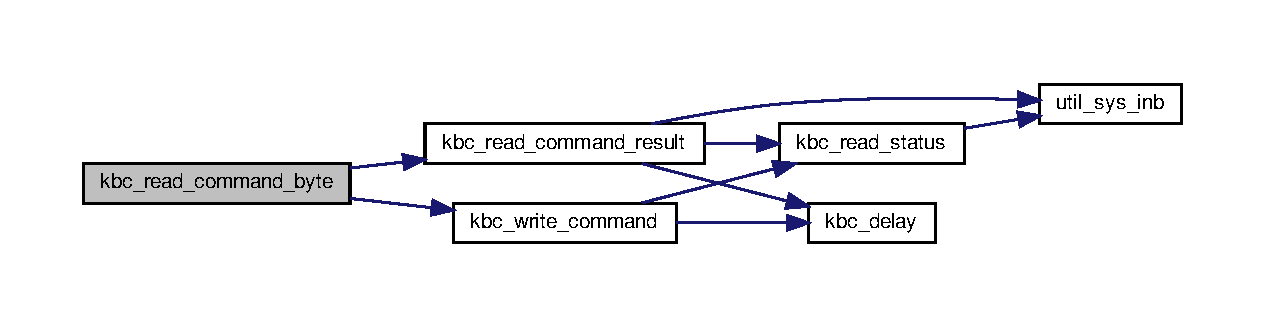
\includegraphics[width=350pt]{group__kbc_gadc6d5fbf9c3a43d168962776591ac75b_cgraph}
\end{center}
\end{figure}
\mbox{\Hypertarget{group__kbc_ga65f11cca39a73154ab68dabac8b12683}\label{group__kbc_ga65f11cca39a73154ab68dabac8b12683}} 
\index{kbc@{kbc}!kbc\+\_\+read\+\_\+command\+\_\+result@{kbc\+\_\+read\+\_\+command\+\_\+result}}
\index{kbc\+\_\+read\+\_\+command\+\_\+result@{kbc\+\_\+read\+\_\+command\+\_\+result}!kbc@{kbc}}
\subsubsection{\texorpdfstring{kbc\+\_\+read\+\_\+command\+\_\+result()}{kbc\_read\_command\_result()}}
{\footnotesize\ttfamily int kbc\+\_\+read\+\_\+command\+\_\+result (\begin{DoxyParamCaption}\item[{uint8\+\_\+t $\ast$}]{result }\end{DoxyParamCaption})}



Reads a command result from the kbc. 


\begin{DoxyParams}{Parameters}
{\em result} & A pointer to the byte which will be rewritten \\
\hline
\end{DoxyParams}
\begin{DoxyReturn}{Returns}
0 if successful, something else otherwise 
\end{DoxyReturn}
Here is the call graph for this function\+:\nopagebreak
\begin{figure}[H]
\begin{center}
\leavevmode
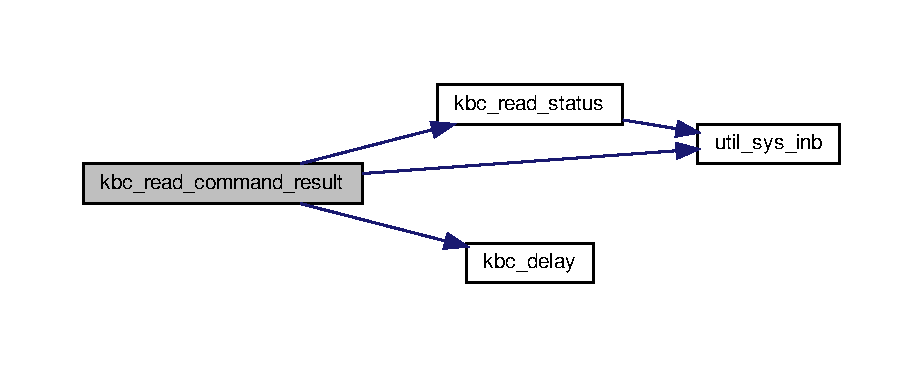
\includegraphics[width=350pt]{group__kbc_ga65f11cca39a73154ab68dabac8b12683_cgraph}
\end{center}
\end{figure}
\mbox{\Hypertarget{group__kbc_gaa4c58a11cd49c54cc0eb02a79010a9cc}\label{group__kbc_gaa4c58a11cd49c54cc0eb02a79010a9cc}} 
\index{kbc@{kbc}!kbc\+\_\+read\+\_\+status@{kbc\+\_\+read\+\_\+status}}
\index{kbc\+\_\+read\+\_\+status@{kbc\+\_\+read\+\_\+status}!kbc@{kbc}}
\subsubsection{\texorpdfstring{kbc\+\_\+read\+\_\+status()}{kbc\_read\_status()}}
{\footnotesize\ttfamily int kbc\+\_\+read\+\_\+status (\begin{DoxyParamCaption}\item[{uint8\+\_\+t $\ast$}]{status }\end{DoxyParamCaption})}



Reads the status of the kbc. 


\begin{DoxyParams}{Parameters}
{\em status} & A pointer to the byte which will be rewritten \\
\hline
\end{DoxyParams}
\begin{DoxyReturn}{Returns}
0 if successful, something else otherwise 
\end{DoxyReturn}
Here is the call graph for this function\+:\nopagebreak
\begin{figure}[H]
\begin{center}
\leavevmode
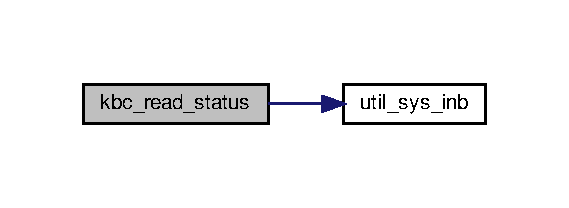
\includegraphics[width=273pt]{group__kbc_gaa4c58a11cd49c54cc0eb02a79010a9cc_cgraph}
\end{center}
\end{figure}
\mbox{\Hypertarget{group__kbc_ga8c467e640bc33719fe3ed7bcb73f2121}\label{group__kbc_ga8c467e640bc33719fe3ed7bcb73f2121}} 
\index{kbc@{kbc}!kbc\+\_\+write\+\_\+command@{kbc\+\_\+write\+\_\+command}}
\index{kbc\+\_\+write\+\_\+command@{kbc\+\_\+write\+\_\+command}!kbc@{kbc}}
\subsubsection{\texorpdfstring{kbc\+\_\+write\+\_\+command()}{kbc\_write\_command()}}
{\footnotesize\ttfamily int kbc\+\_\+write\+\_\+command (\begin{DoxyParamCaption}\item[{uint8\+\_\+t}]{command }\end{DoxyParamCaption})}



Sends a command to the kbc. 


\begin{DoxyParams}{Parameters}
{\em command} & The command byte to be sent \\
\hline
\end{DoxyParams}
\begin{DoxyReturn}{Returns}
0 if successful, something else otherwise 
\end{DoxyReturn}
Here is the call graph for this function\+:\nopagebreak
\begin{figure}[H]
\begin{center}
\leavevmode
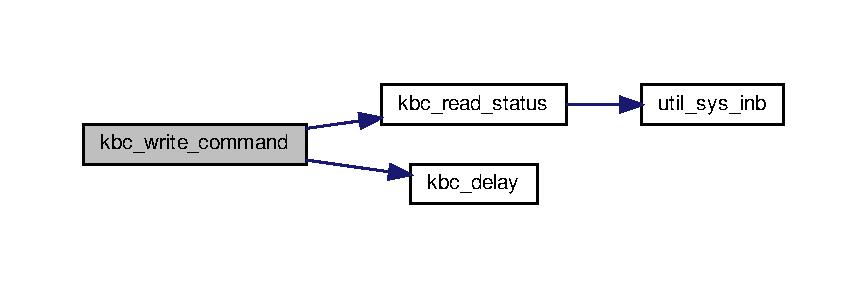
\includegraphics[width=350pt]{group__kbc_ga8c467e640bc33719fe3ed7bcb73f2121_cgraph}
\end{center}
\end{figure}
\mbox{\Hypertarget{group__kbc_ga24f1a4d1bcb60a73ebd6cee462191a52}\label{group__kbc_ga24f1a4d1bcb60a73ebd6cee462191a52}} 
\index{kbc@{kbc}!kbc\+\_\+write\+\_\+command\+\_\+arg@{kbc\+\_\+write\+\_\+command\+\_\+arg}}
\index{kbc\+\_\+write\+\_\+command\+\_\+arg@{kbc\+\_\+write\+\_\+command\+\_\+arg}!kbc@{kbc}}
\subsubsection{\texorpdfstring{kbc\+\_\+write\+\_\+command\+\_\+arg()}{kbc\_write\_command\_arg()}}
{\footnotesize\ttfamily int kbc\+\_\+write\+\_\+command\+\_\+arg (\begin{DoxyParamCaption}\item[{uint8\+\_\+t}]{arg }\end{DoxyParamCaption})}



Sends an argument to the kbc. 


\begin{DoxyParams}{Parameters}
{\em arg} & The argument byte to be sent \\
\hline
\end{DoxyParams}
\begin{DoxyReturn}{Returns}
0 if successful, something else otherwise 
\end{DoxyReturn}
Here is the call graph for this function\+:\nopagebreak
\begin{figure}[H]
\begin{center}
\leavevmode
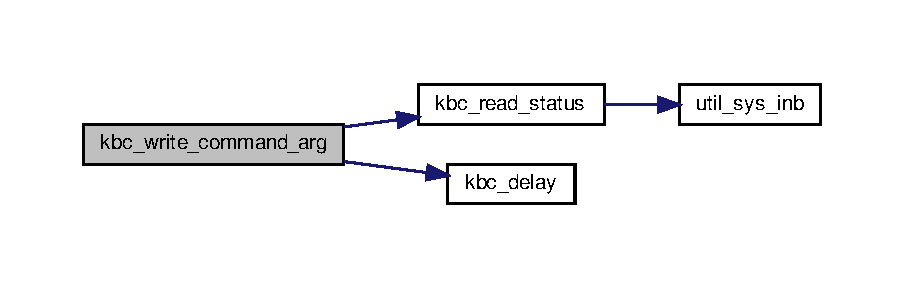
\includegraphics[width=350pt]{group__kbc_ga24f1a4d1bcb60a73ebd6cee462191a52_cgraph}
\end{center}
\end{figure}
\mbox{\Hypertarget{group__kbc_ga5e840dccbbe5abccff8ca66f78c476c9}\label{group__kbc_ga5e840dccbbe5abccff8ca66f78c476c9}} 
\index{kbc@{kbc}!kbc\+\_\+write\+\_\+command\+\_\+byte@{kbc\+\_\+write\+\_\+command\+\_\+byte}}
\index{kbc\+\_\+write\+\_\+command\+\_\+byte@{kbc\+\_\+write\+\_\+command\+\_\+byte}!kbc@{kbc}}
\subsubsection{\texorpdfstring{kbc\+\_\+write\+\_\+command\+\_\+byte()}{kbc\_write\_command\_byte()}}
{\footnotesize\ttfamily int kbc\+\_\+write\+\_\+command\+\_\+byte (\begin{DoxyParamCaption}\item[{uint8\+\_\+t}]{command\+\_\+byte }\end{DoxyParamCaption})}



Sends a command byte to the kbc. 


\begin{DoxyParams}{Parameters}
{\em command\+\_\+byte} & The command byte to be sent \\
\hline
\end{DoxyParams}
\begin{DoxyReturn}{Returns}
0 if successful, something else otherwise 
\end{DoxyReturn}
Here is the call graph for this function\+:\nopagebreak
\begin{figure}[H]
\begin{center}
\leavevmode
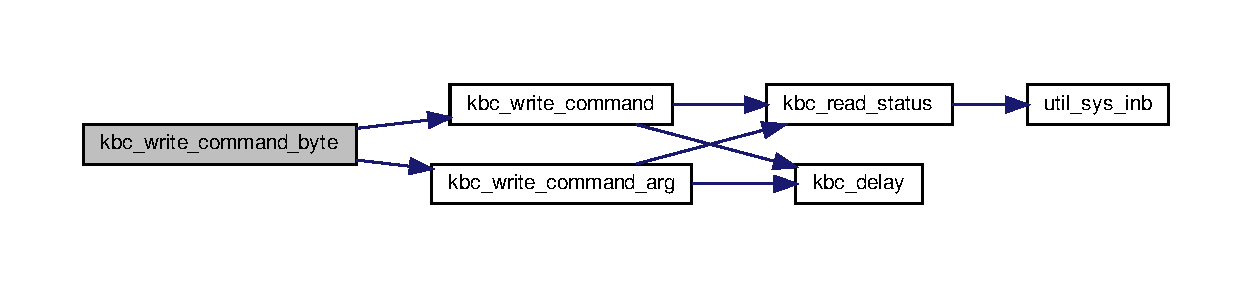
\includegraphics[width=350pt]{group__kbc_ga5e840dccbbe5abccff8ca66f78c476c9_cgraph}
\end{center}
\end{figure}

\hypertarget{group__keyboard}{}\section{keyboard}
\label{group__keyboard}\index{keyboard@{keyboard}}


Keyboard-\/related interrupt functions.  


\subsection*{Data Structures}
\begin{DoxyCompactItemize}
\item 
struct \hyperlink{structkeyboard__packet}{keyboard\+\_\+packet}
\begin{DoxyCompactList}\small\item\em Struct that represents a keyboard packet. \end{DoxyCompactList}\end{DoxyCompactItemize}
\subsection*{Macros}
\begin{DoxyCompactItemize}
\item 
\#define \hyperlink{group__keyboard_ga2d17911b50c0aeebb2e3325c5b36d4f2}{K\+E\+Y\+B\+O\+A\+R\+D\+\_\+\+I\+RQ}~1
\item 
\#define \hyperlink{group__keyboard_ga03c0bb70d0f678541f822faab96376bc}{K\+E\+Y\+B\+O\+A\+R\+D\+\_\+\+H\+O\+O\+K\+\_\+\+ID}~1
\item 
\#define \hyperlink{group__keyboard_ga67f9ce144f998dd5c8b1ae5e25fb8dec}{K\+E\+Y\+B\+O\+A\+R\+D\+\_\+\+M\+A\+SK}~B\+IT(\hyperlink{group__keyboard_ga03c0bb70d0f678541f822faab96376bc}{K\+E\+Y\+B\+O\+A\+R\+D\+\_\+\+H\+O\+O\+K\+\_\+\+ID})
\item 
\#define \hyperlink{group__keyboard_gaa639f3ee505b0f62686d71087830b1d5}{K\+E\+Y\+B\+O\+A\+R\+D\+\_\+\+T\+W\+O\+\_\+\+B\+Y\+T\+E\+S\+\_\+\+M\+SB}~0x\+E0
\end{DoxyCompactItemize}
\subsection*{Typedefs}
\begin{DoxyCompactItemize}
\item 
typedef struct \hyperlink{structkeyboard__packet}{keyboard\+\_\+packet} \hyperlink{group__keyboard_ga823c244c9bc4e1f5004a548133e112d9}{keyboard\+\_\+packet}
\begin{DoxyCompactList}\small\item\em Struct that represents a keyboard packet. \end{DoxyCompactList}\end{DoxyCompactItemize}
\subsection*{Functions}
\begin{DoxyCompactItemize}
\item 
bool \hyperlink{group__keyboard_ga92937e5072f297d330bd57bb62cd35fb}{keyboard\+\_\+ih2} (\hyperlink{structkeyboard__packet}{keyboard\+\_\+packet} $\ast$new\+\_\+packet)
\begin{DoxyCompactList}\small\item\em The second part of keyboard interrupt handling. \end{DoxyCompactList}\item 
int \hyperlink{group__keyboard_ga73e07d998291eb412f8097fd06ddafa8}{keyboard\+\_\+ih\+\_\+subscribe} ()
\begin{DoxyCompactList}\small\item\em Subscribes to keyboard interrupts. \end{DoxyCompactList}\item 
int \hyperlink{group__keyboard_gae7dcc7462f98df72164f4a194125d0e9}{keyboard\+\_\+ih\+\_\+unsubscribe} ()
\begin{DoxyCompactList}\small\item\em Unsubscribes to keyboard interrupts. \end{DoxyCompactList}\item 
int \hyperlink{group__keyboard_gad416a0ec7ca419806341ab7be70064b1}{keyboard\+\_\+ih\+\_\+enable} ()
\begin{DoxyCompactList}\small\item\em Enables keyboard interrupts. \end{DoxyCompactList}\item 
int \hyperlink{group__keyboard_ga803d759506fefe9119ad529c783b3a7a}{keyboard\+\_\+ih\+\_\+disable} ()
\begin{DoxyCompactList}\small\item\em Disables keyboard interrupts. \end{DoxyCompactList}\end{DoxyCompactItemize}


\subsection{Detailed Description}
Keyboard-\/related interrupt functions. 



\subsection{Macro Definition Documentation}
\mbox{\Hypertarget{group__keyboard_ga03c0bb70d0f678541f822faab96376bc}\label{group__keyboard_ga03c0bb70d0f678541f822faab96376bc}} 
\index{keyboard@{keyboard}!K\+E\+Y\+B\+O\+A\+R\+D\+\_\+\+H\+O\+O\+K\+\_\+\+ID@{K\+E\+Y\+B\+O\+A\+R\+D\+\_\+\+H\+O\+O\+K\+\_\+\+ID}}
\index{K\+E\+Y\+B\+O\+A\+R\+D\+\_\+\+H\+O\+O\+K\+\_\+\+ID@{K\+E\+Y\+B\+O\+A\+R\+D\+\_\+\+H\+O\+O\+K\+\_\+\+ID}!keyboard@{keyboard}}
\subsubsection{\texorpdfstring{K\+E\+Y\+B\+O\+A\+R\+D\+\_\+\+H\+O\+O\+K\+\_\+\+ID}{KEYBOARD\_HOOK\_ID}}
{\footnotesize\ttfamily \#define K\+E\+Y\+B\+O\+A\+R\+D\+\_\+\+H\+O\+O\+K\+\_\+\+ID~1}

\mbox{\Hypertarget{group__keyboard_ga2d17911b50c0aeebb2e3325c5b36d4f2}\label{group__keyboard_ga2d17911b50c0aeebb2e3325c5b36d4f2}} 
\index{keyboard@{keyboard}!K\+E\+Y\+B\+O\+A\+R\+D\+\_\+\+I\+RQ@{K\+E\+Y\+B\+O\+A\+R\+D\+\_\+\+I\+RQ}}
\index{K\+E\+Y\+B\+O\+A\+R\+D\+\_\+\+I\+RQ@{K\+E\+Y\+B\+O\+A\+R\+D\+\_\+\+I\+RQ}!keyboard@{keyboard}}
\subsubsection{\texorpdfstring{K\+E\+Y\+B\+O\+A\+R\+D\+\_\+\+I\+RQ}{KEYBOARD\_IRQ}}
{\footnotesize\ttfamily \#define K\+E\+Y\+B\+O\+A\+R\+D\+\_\+\+I\+RQ~1}

\mbox{\Hypertarget{group__keyboard_ga67f9ce144f998dd5c8b1ae5e25fb8dec}\label{group__keyboard_ga67f9ce144f998dd5c8b1ae5e25fb8dec}} 
\index{keyboard@{keyboard}!K\+E\+Y\+B\+O\+A\+R\+D\+\_\+\+M\+A\+SK@{K\+E\+Y\+B\+O\+A\+R\+D\+\_\+\+M\+A\+SK}}
\index{K\+E\+Y\+B\+O\+A\+R\+D\+\_\+\+M\+A\+SK@{K\+E\+Y\+B\+O\+A\+R\+D\+\_\+\+M\+A\+SK}!keyboard@{keyboard}}
\subsubsection{\texorpdfstring{K\+E\+Y\+B\+O\+A\+R\+D\+\_\+\+M\+A\+SK}{KEYBOARD\_MASK}}
{\footnotesize\ttfamily \#define K\+E\+Y\+B\+O\+A\+R\+D\+\_\+\+M\+A\+SK~B\+IT(\hyperlink{group__keyboard_ga03c0bb70d0f678541f822faab96376bc}{K\+E\+Y\+B\+O\+A\+R\+D\+\_\+\+H\+O\+O\+K\+\_\+\+ID})}

\mbox{\Hypertarget{group__keyboard_gaa639f3ee505b0f62686d71087830b1d5}\label{group__keyboard_gaa639f3ee505b0f62686d71087830b1d5}} 
\index{keyboard@{keyboard}!K\+E\+Y\+B\+O\+A\+R\+D\+\_\+\+T\+W\+O\+\_\+\+B\+Y\+T\+E\+S\+\_\+\+M\+SB@{K\+E\+Y\+B\+O\+A\+R\+D\+\_\+\+T\+W\+O\+\_\+\+B\+Y\+T\+E\+S\+\_\+\+M\+SB}}
\index{K\+E\+Y\+B\+O\+A\+R\+D\+\_\+\+T\+W\+O\+\_\+\+B\+Y\+T\+E\+S\+\_\+\+M\+SB@{K\+E\+Y\+B\+O\+A\+R\+D\+\_\+\+T\+W\+O\+\_\+\+B\+Y\+T\+E\+S\+\_\+\+M\+SB}!keyboard@{keyboard}}
\subsubsection{\texorpdfstring{K\+E\+Y\+B\+O\+A\+R\+D\+\_\+\+T\+W\+O\+\_\+\+B\+Y\+T\+E\+S\+\_\+\+M\+SB}{KEYBOARD\_TWO\_BYTES\_MSB}}
{\footnotesize\ttfamily \#define K\+E\+Y\+B\+O\+A\+R\+D\+\_\+\+T\+W\+O\+\_\+\+B\+Y\+T\+E\+S\+\_\+\+M\+SB~0x\+E0}



\subsection{Typedef Documentation}
\mbox{\Hypertarget{group__keyboard_ga823c244c9bc4e1f5004a548133e112d9}\label{group__keyboard_ga823c244c9bc4e1f5004a548133e112d9}} 
\index{keyboard@{keyboard}!keyboard\+\_\+packet@{keyboard\+\_\+packet}}
\index{keyboard\+\_\+packet@{keyboard\+\_\+packet}!keyboard@{keyboard}}
\subsubsection{\texorpdfstring{keyboard\+\_\+packet}{keyboard\_packet}}
{\footnotesize\ttfamily typedef struct \hyperlink{structkeyboard__packet}{keyboard\+\_\+packet}  \hyperlink{structkeyboard__packet}{keyboard\+\_\+packet}}



Struct that represents a keyboard packet. 



\subsection{Function Documentation}
\mbox{\Hypertarget{group__keyboard_ga92937e5072f297d330bd57bb62cd35fb}\label{group__keyboard_ga92937e5072f297d330bd57bb62cd35fb}} 
\index{keyboard@{keyboard}!keyboard\+\_\+ih2@{keyboard\+\_\+ih2}}
\index{keyboard\+\_\+ih2@{keyboard\+\_\+ih2}!keyboard@{keyboard}}
\subsubsection{\texorpdfstring{keyboard\+\_\+ih2()}{keyboard\_ih2()}}
{\footnotesize\ttfamily bool keyboard\+\_\+ih2 (\begin{DoxyParamCaption}\item[{\hyperlink{structkeyboard__packet}{keyboard\+\_\+packet} $\ast$}]{new\+\_\+packet }\end{DoxyParamCaption})}



The second part of keyboard interrupt handling. 

Calls to this function should be preceded immediately by \hyperlink{keyboard_8c_a5761bd4aad91ac1d68916ad88f583d9f}{kbc\+\_\+ih(void)}


\begin{DoxyParams}{Parameters}
{\em new\+\_\+packet} & A \hyperlink{structkeyboard__packet}{keyboard\+\_\+packet} pointer that will get overwritten if the packet was fully parsed \\
\hline
\end{DoxyParams}
\begin{DoxyReturn}{Returns}
true if the packet was overwritten with a new packet, otherwise false 
\end{DoxyReturn}
\mbox{\Hypertarget{group__keyboard_ga803d759506fefe9119ad529c783b3a7a}\label{group__keyboard_ga803d759506fefe9119ad529c783b3a7a}} 
\index{keyboard@{keyboard}!keyboard\+\_\+ih\+\_\+disable@{keyboard\+\_\+ih\+\_\+disable}}
\index{keyboard\+\_\+ih\+\_\+disable@{keyboard\+\_\+ih\+\_\+disable}!keyboard@{keyboard}}
\subsubsection{\texorpdfstring{keyboard\+\_\+ih\+\_\+disable()}{keyboard\_ih\_disable()}}
{\footnotesize\ttfamily int keyboard\+\_\+ih\+\_\+disable (\begin{DoxyParamCaption}{ }\end{DoxyParamCaption})}



Disables keyboard interrupts. 

\begin{DoxyReturn}{Returns}
0 if successful, otherwise it was not successful 
\end{DoxyReturn}
\mbox{\Hypertarget{group__keyboard_gad416a0ec7ca419806341ab7be70064b1}\label{group__keyboard_gad416a0ec7ca419806341ab7be70064b1}} 
\index{keyboard@{keyboard}!keyboard\+\_\+ih\+\_\+enable@{keyboard\+\_\+ih\+\_\+enable}}
\index{keyboard\+\_\+ih\+\_\+enable@{keyboard\+\_\+ih\+\_\+enable}!keyboard@{keyboard}}
\subsubsection{\texorpdfstring{keyboard\+\_\+ih\+\_\+enable()}{keyboard\_ih\_enable()}}
{\footnotesize\ttfamily int keyboard\+\_\+ih\+\_\+enable (\begin{DoxyParamCaption}{ }\end{DoxyParamCaption})}



Enables keyboard interrupts. 

\begin{DoxyReturn}{Returns}
0 if successful, otherwise it was not successful 
\end{DoxyReturn}
\mbox{\Hypertarget{group__keyboard_ga73e07d998291eb412f8097fd06ddafa8}\label{group__keyboard_ga73e07d998291eb412f8097fd06ddafa8}} 
\index{keyboard@{keyboard}!keyboard\+\_\+ih\+\_\+subscribe@{keyboard\+\_\+ih\+\_\+subscribe}}
\index{keyboard\+\_\+ih\+\_\+subscribe@{keyboard\+\_\+ih\+\_\+subscribe}!keyboard@{keyboard}}
\subsubsection{\texorpdfstring{keyboard\+\_\+ih\+\_\+subscribe()}{keyboard\_ih\_subscribe()}}
{\footnotesize\ttfamily int keyboard\+\_\+ih\+\_\+subscribe (\begin{DoxyParamCaption}{ }\end{DoxyParamCaption})}



Subscribes to keyboard interrupts. 

\begin{DoxyReturn}{Returns}
0 if successful, otherwise it was not successful 
\end{DoxyReturn}
\mbox{\Hypertarget{group__keyboard_gae7dcc7462f98df72164f4a194125d0e9}\label{group__keyboard_gae7dcc7462f98df72164f4a194125d0e9}} 
\index{keyboard@{keyboard}!keyboard\+\_\+ih\+\_\+unsubscribe@{keyboard\+\_\+ih\+\_\+unsubscribe}}
\index{keyboard\+\_\+ih\+\_\+unsubscribe@{keyboard\+\_\+ih\+\_\+unsubscribe}!keyboard@{keyboard}}
\subsubsection{\texorpdfstring{keyboard\+\_\+ih\+\_\+unsubscribe()}{keyboard\_ih\_unsubscribe()}}
{\footnotesize\ttfamily int keyboard\+\_\+ih\+\_\+unsubscribe (\begin{DoxyParamCaption}{ }\end{DoxyParamCaption})}



Unsubscribes to keyboard interrupts. 

\begin{DoxyReturn}{Returns}
0 if successful, otherwise it was not successful 
\end{DoxyReturn}

\hypertarget{group___menu}{}\section{Menu}
\label{group___menu}\index{Menu@{Menu}}


Menu-\/related functions.  


\subsection*{Functions}
\begin{DoxyCompactItemize}
\item 
void \hyperlink{group___menu_ga730cfddc7cb680e1b1d4ad54d4a8be30}{set\+\_\+rectangle\+\_\+frame} (uint8\+\_\+t $\ast$base\+\_\+ptr, uint16\+\_\+t x, uint16\+\_\+t y, uint16\+\_\+t len\+\_\+x, uint16\+\_\+t len\+\_\+y, uint16\+\_\+t len\+\_\+edge, uint32\+\_\+t color)
\begin{DoxyCompactList}\small\item\em It draws the frame of a rectangle, used for buttons. \end{DoxyCompactList}\item 
void \hyperlink{group___menu_gaa59cc81964587bdbe8dcd981e8e6fd08}{load\+\_\+xpm\+\_\+menu} ()
\begin{DoxyCompactList}\small\item\em Loads the X\+P\+Ms for the menus, if they have not been already loaded. \end{DoxyCompactList}\item 
void \hyperlink{group___menu_ga06326bc3ce2fdfe90cb6eb3172159fd0}{draw\+Main\+Menu} ()
\begin{DoxyCompactList}\small\item\em Draws the main menu with the options\+: play, help, options and exit. It also displays the current time. \end{DoxyCompactList}\item 
void \hyperlink{group___menu_ga879287e331940c91b6b6b9dbb65474de}{draw\+Help\+Menu} ()
\begin{DoxyCompactList}\small\item\em Draws the help menu that explains the players\textquotesingle{} commands. \end{DoxyCompactList}\item 
void \hyperlink{group___menu_ga8be4d848c58721f26653059357806041}{draw\+Options\+Menu} ()
\begin{DoxyCompactList}\small\item\em Draws the options menu that allows the players to change some settings like if the player s want bouncy walls, infinite ammo, be affected by gravity and if they want wall damage. \end{DoxyCompactList}\item 
bool \hyperlink{group___menu_ga24808d404d0ba3711a2445fc0d876167}{checkpixel\+\_\+inbutton} (uint16\+\_\+t pixel\+\_\+x, uint16\+\_\+t pixel\+\_\+y, uint16\+\_\+t x, uint16\+\_\+t y, uint16\+\_\+t len\+\_\+x, uint16\+\_\+t len\+\_\+y)
\begin{DoxyCompactList}\small\item\em Checks if a pixel is inside a rectangle. \end{DoxyCompactList}\end{DoxyCompactItemize}


\subsection{Detailed Description}
Menu-\/related functions. 



\subsection{Function Documentation}
\mbox{\Hypertarget{group___menu_ga24808d404d0ba3711a2445fc0d876167}\label{group___menu_ga24808d404d0ba3711a2445fc0d876167}} 
\index{Menu@{Menu}!checkpixel\+\_\+inbutton@{checkpixel\+\_\+inbutton}}
\index{checkpixel\+\_\+inbutton@{checkpixel\+\_\+inbutton}!Menu@{Menu}}
\subsubsection{\texorpdfstring{checkpixel\+\_\+inbutton()}{checkpixel\_inbutton()}}
{\footnotesize\ttfamily bool checkpixel\+\_\+inbutton (\begin{DoxyParamCaption}\item[{uint16\+\_\+t}]{pixel\+\_\+x,  }\item[{uint16\+\_\+t}]{pixel\+\_\+y,  }\item[{uint16\+\_\+t}]{x,  }\item[{uint16\+\_\+t}]{y,  }\item[{uint16\+\_\+t}]{len\+\_\+x,  }\item[{uint16\+\_\+t}]{len\+\_\+y }\end{DoxyParamCaption})}



Checks if a pixel is inside a rectangle. 


\begin{DoxyParams}{Parameters}
{\em pixel\+\_\+x} & The x coordenate of the pixel \\
\hline
{\em pixel\+\_\+y} & The y coordenate of the pixel \\
\hline
{\em x} & The x coordinate of the top left corner of the rectangle (counting downwards from the top) \\
\hline
{\em y} & The y coordinate of the top left corner of the rectangle (counting rightwards from the left) \\
\hline
{\em len\+\_\+x} & The width of the rectangle \\
\hline
{\em len\+\_\+y} & The height of the rectangle \\
\hline
\end{DoxyParams}
\mbox{\Hypertarget{group___menu_ga879287e331940c91b6b6b9dbb65474de}\label{group___menu_ga879287e331940c91b6b6b9dbb65474de}} 
\index{Menu@{Menu}!draw\+Help\+Menu@{draw\+Help\+Menu}}
\index{draw\+Help\+Menu@{draw\+Help\+Menu}!Menu@{Menu}}
\subsubsection{\texorpdfstring{draw\+Help\+Menu()}{drawHelpMenu()}}
{\footnotesize\ttfamily void draw\+Help\+Menu (\begin{DoxyParamCaption}{ }\end{DoxyParamCaption})}



Draws the help menu that explains the players\textquotesingle{} commands. 

Here is the call graph for this function\+:\nopagebreak
\begin{figure}[H]
\begin{center}
\leavevmode
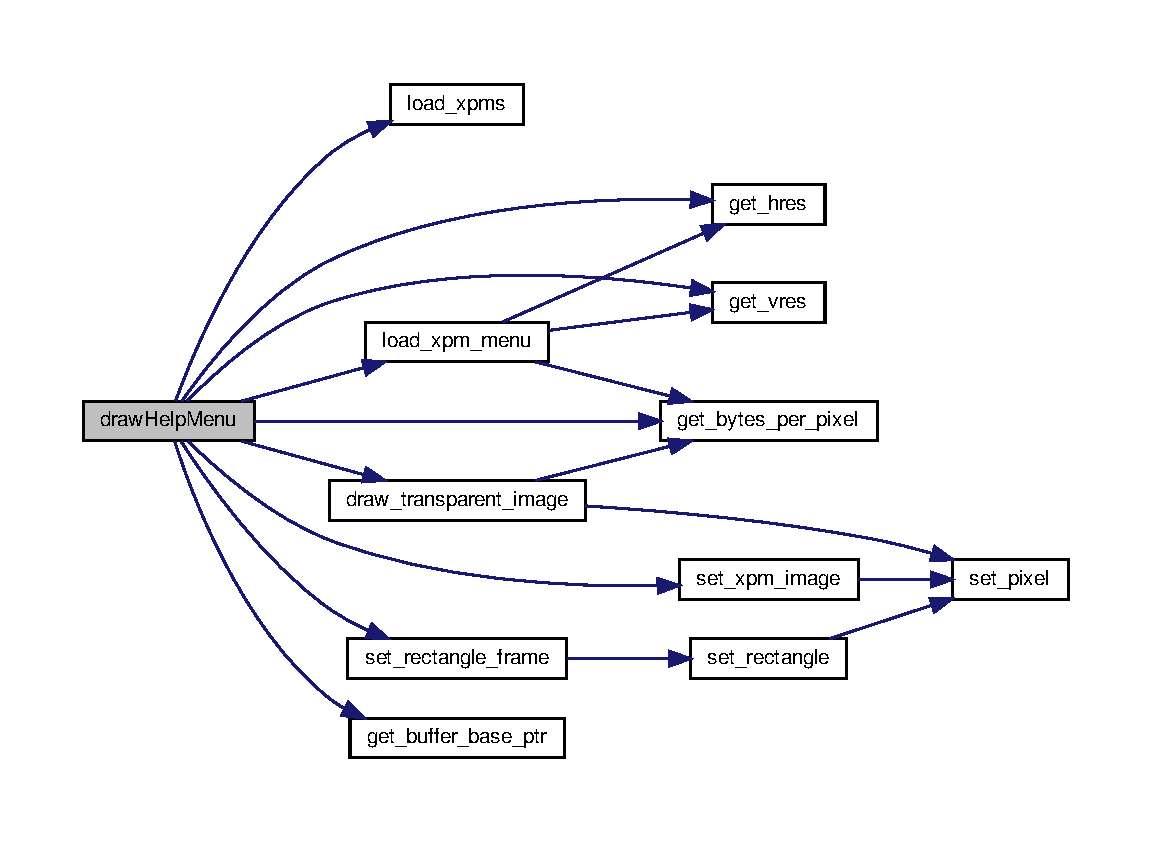
\includegraphics[width=350pt]{group___menu_ga879287e331940c91b6b6b9dbb65474de_cgraph}
\end{center}
\end{figure}
\mbox{\Hypertarget{group___menu_ga06326bc3ce2fdfe90cb6eb3172159fd0}\label{group___menu_ga06326bc3ce2fdfe90cb6eb3172159fd0}} 
\index{Menu@{Menu}!draw\+Main\+Menu@{draw\+Main\+Menu}}
\index{draw\+Main\+Menu@{draw\+Main\+Menu}!Menu@{Menu}}
\subsubsection{\texorpdfstring{draw\+Main\+Menu()}{drawMainMenu()}}
{\footnotesize\ttfamily void draw\+Main\+Menu (\begin{DoxyParamCaption}{ }\end{DoxyParamCaption})}



Draws the main menu with the options\+: play, help, options and exit. It also displays the current time. 

Here is the call graph for this function\+:\nopagebreak
\begin{figure}[H]
\begin{center}
\leavevmode
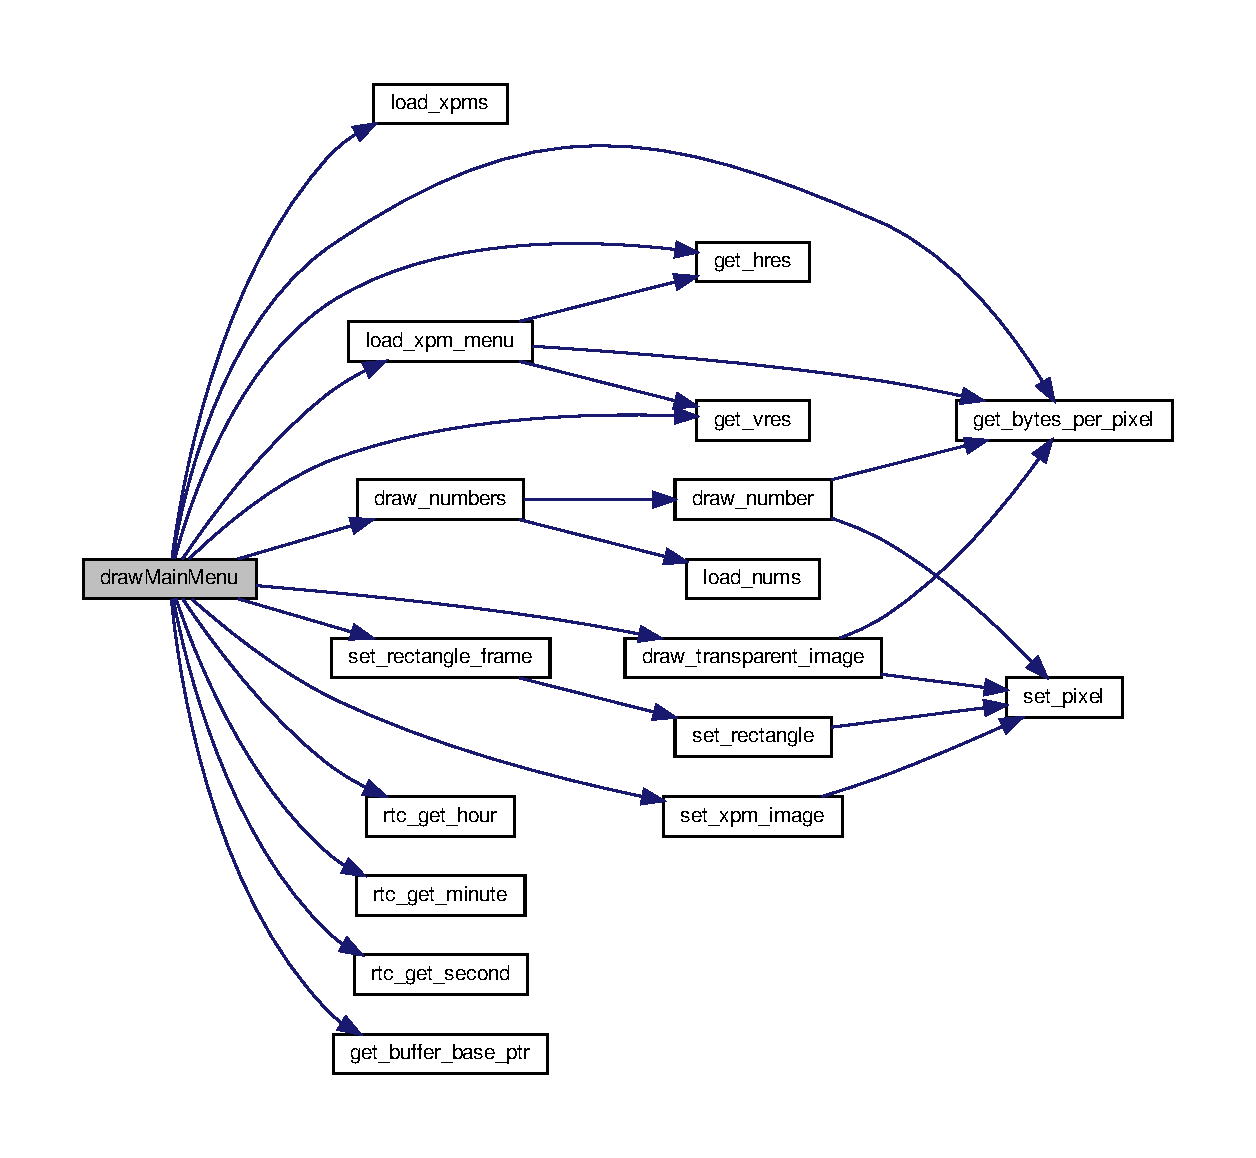
\includegraphics[width=350pt]{group___menu_ga06326bc3ce2fdfe90cb6eb3172159fd0_cgraph}
\end{center}
\end{figure}
\mbox{\Hypertarget{group___menu_ga8be4d848c58721f26653059357806041}\label{group___menu_ga8be4d848c58721f26653059357806041}} 
\index{Menu@{Menu}!draw\+Options\+Menu@{draw\+Options\+Menu}}
\index{draw\+Options\+Menu@{draw\+Options\+Menu}!Menu@{Menu}}
\subsubsection{\texorpdfstring{draw\+Options\+Menu()}{drawOptionsMenu()}}
{\footnotesize\ttfamily void draw\+Options\+Menu (\begin{DoxyParamCaption}{ }\end{DoxyParamCaption})}



Draws the options menu that allows the players to change some settings like if the player s want bouncy walls, infinite ammo, be affected by gravity and if they want wall damage. 

Here is the call graph for this function\+:\nopagebreak
\begin{figure}[H]
\begin{center}
\leavevmode
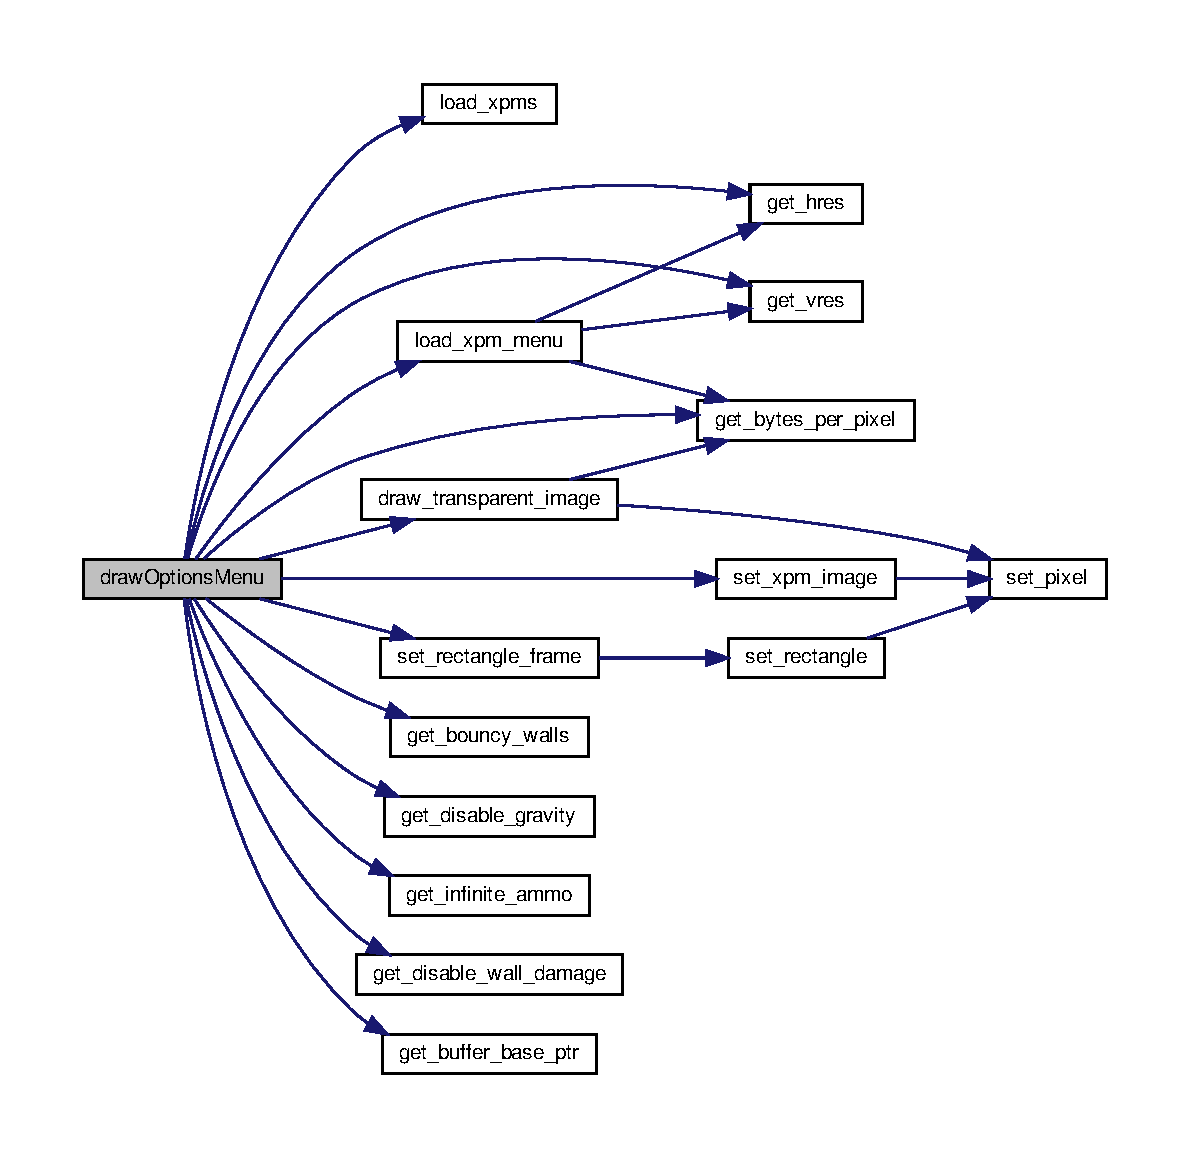
\includegraphics[width=350pt]{group___menu_ga8be4d848c58721f26653059357806041_cgraph}
\end{center}
\end{figure}
\mbox{\Hypertarget{group___menu_gaa59cc81964587bdbe8dcd981e8e6fd08}\label{group___menu_gaa59cc81964587bdbe8dcd981e8e6fd08}} 
\index{Menu@{Menu}!load\+\_\+xpm\+\_\+menu@{load\+\_\+xpm\+\_\+menu}}
\index{load\+\_\+xpm\+\_\+menu@{load\+\_\+xpm\+\_\+menu}!Menu@{Menu}}
\subsubsection{\texorpdfstring{load\+\_\+xpm\+\_\+menu()}{load\_xpm\_menu()}}
{\footnotesize\ttfamily void load\+\_\+xpm\+\_\+menu (\begin{DoxyParamCaption}{ }\end{DoxyParamCaption})}



Loads the X\+P\+Ms for the menus, if they have not been already loaded. 

Here is the call graph for this function\+:\nopagebreak
\begin{figure}[H]
\begin{center}
\leavevmode
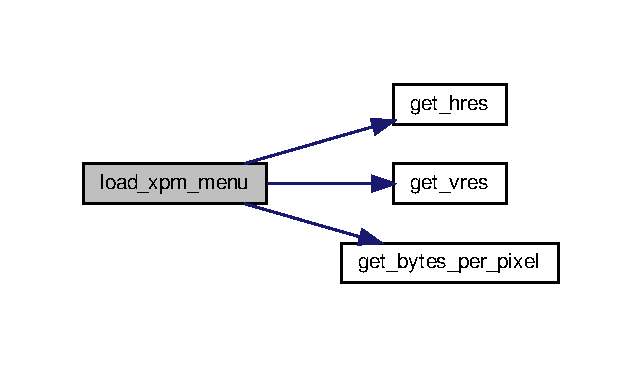
\includegraphics[width=308pt]{group___menu_gaa59cc81964587bdbe8dcd981e8e6fd08_cgraph}
\end{center}
\end{figure}
\mbox{\Hypertarget{group___menu_ga730cfddc7cb680e1b1d4ad54d4a8be30}\label{group___menu_ga730cfddc7cb680e1b1d4ad54d4a8be30}} 
\index{Menu@{Menu}!set\+\_\+rectangle\+\_\+frame@{set\+\_\+rectangle\+\_\+frame}}
\index{set\+\_\+rectangle\+\_\+frame@{set\+\_\+rectangle\+\_\+frame}!Menu@{Menu}}
\subsubsection{\texorpdfstring{set\+\_\+rectangle\+\_\+frame()}{set\_rectangle\_frame()}}
{\footnotesize\ttfamily void set\+\_\+rectangle\+\_\+frame (\begin{DoxyParamCaption}\item[{uint8\+\_\+t $\ast$}]{base\+\_\+ptr,  }\item[{uint16\+\_\+t}]{x,  }\item[{uint16\+\_\+t}]{y,  }\item[{uint16\+\_\+t}]{len\+\_\+x,  }\item[{uint16\+\_\+t}]{len\+\_\+y,  }\item[{uint16\+\_\+t}]{len\+\_\+edge,  }\item[{uint32\+\_\+t}]{color }\end{DoxyParamCaption})}



It draws the frame of a rectangle, used for buttons. 


\begin{DoxyParams}{Parameters}
{\em base\+\_\+ptr} & A pointer to a buffer (must be equal in size to the frame buffer) \\
\hline
{\em x} & The x coordinate of the top left corner of the rectangle (counting downwards from the top) \\
\hline
{\em y} & The y coordinate of the top left corner of the rectangle (counting rightwards from the left) \\
\hline
{\em len\+\_\+x} & The width of the rectangle \\
\hline
{\em len\+\_\+y} & The height of the rectangle \\
\hline
{\em len\+\_\+edge} & The depth of the frame \\
\hline
{\em color} & The color of the rectangle \\
\hline
\end{DoxyParams}
Here is the call graph for this function\+:\nopagebreak
\begin{figure}[H]
\begin{center}
\leavevmode
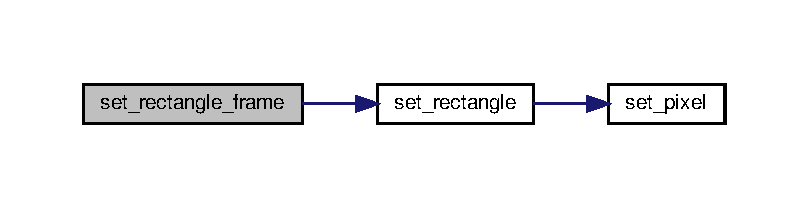
\includegraphics[width=350pt]{group___menu_ga730cfddc7cb680e1b1d4ad54d4a8be30_cgraph}
\end{center}
\end{figure}

\hypertarget{group__mouse}{}\section{mouse}
\label{group__mouse}\index{mouse@{mouse}}


Mouse-\/related interrupt and command-\/sending functions.  


\subsection*{Data Structures}
\begin{DoxyCompactItemize}
\item 
struct \hyperlink{structmouse__packet}{mouse\+\_\+packet}
\begin{DoxyCompactList}\small\item\em Struct that represents a mouse packet. This struct was provided by one of L\+C\+OM\textquotesingle{}s header files. \end{DoxyCompactList}\end{DoxyCompactItemize}
\subsection*{Macros}
\begin{DoxyCompactItemize}
\item 
\#define \hyperlink{group__mouse_ga85964cb90343bb1a029b1d1b4229f910}{M\+O\+U\+S\+E\+\_\+\+I\+RQ}~12
\item 
\#define \hyperlink{group__mouse_gab68ffa76160866a0585aead19b67a130}{M\+O\+U\+S\+E\+\_\+\+H\+O\+O\+K\+\_\+\+ID}~2
\item 
\#define \hyperlink{group__mouse_ga3827dd7e924d260f38f9d045860f1cbd}{M\+O\+U\+S\+E\+\_\+\+M\+A\+SK}~B\+IT(\hyperlink{group__mouse_gab68ffa76160866a0585aead19b67a130}{M\+O\+U\+S\+E\+\_\+\+H\+O\+O\+K\+\_\+\+ID})
\item 
\#define \hyperlink{group__mouse_gae4fd8309d3740444324d85d2ac44beff}{M\+O\+U\+S\+E\+\_\+\+B\+Y\+T\+E\+\_\+1\+\_\+\+Y\+\_\+\+O\+V\+FL}~B\+IT(7)
\item 
\#define \hyperlink{group__mouse_ga9495aababa14763f72d708ce1fe00688}{M\+O\+U\+S\+E\+\_\+\+B\+Y\+T\+E\+\_\+1\+\_\+\+X\+\_\+\+O\+V\+FL}~B\+IT(6)
\item 
\#define \hyperlink{group__mouse_ga40a1d41abbb3d62b78a17c787e42b1a1}{M\+O\+U\+S\+E\+\_\+\+B\+Y\+T\+E\+\_\+1\+\_\+\+M\+S\+B\+\_\+\+Y\+\_\+\+D\+E\+L\+TA}~B\+IT(5)
\item 
\#define \hyperlink{group__mouse_gaa99d2d0eb460df4a2de767cb1ccf9821}{M\+O\+U\+S\+E\+\_\+\+B\+Y\+T\+E\+\_\+1\+\_\+\+M\+S\+B\+\_\+\+X\+\_\+\+D\+E\+L\+TA}~B\+IT(4)
\item 
\#define \hyperlink{group__mouse_ga02a6dbb607416ec197dadeadda1d1a0f}{M\+O\+U\+S\+E\+\_\+\+B\+Y\+T\+E\+\_\+1\+\_\+\+B\+I\+T\+\_\+\+S\+E\+T\+\_\+\+T\+O\+\_\+1}~B\+IT(3)
\item 
\#define \hyperlink{group__mouse_ga0ff3caa0262caf3650e60bef9e7ee7af}{M\+O\+U\+S\+E\+\_\+\+B\+Y\+T\+E\+\_\+1\+\_\+\+MB}~B\+IT(2)
\item 
\#define \hyperlink{group__mouse_ga192e557f1c7e34d6f7819950f2d13f5a}{M\+O\+U\+S\+E\+\_\+\+B\+Y\+T\+E\+\_\+1\+\_\+\+RB}~B\+IT(1)
\item 
\#define \hyperlink{group__mouse_gac52085fb9fe5541384e6da6fc2a1d25d}{M\+O\+U\+S\+E\+\_\+\+B\+Y\+T\+E\+\_\+1\+\_\+\+LB}~B\+IT(0)
\item 
\#define \hyperlink{group__mouse_ga0c74c250143abeeac88e08d0e3834124}{M\+O\+U\+S\+E\+\_\+\+C\+O\+M\+\_\+\+R\+E\+S\+ET}~0x\+FF
\item 
\#define \hyperlink{group__mouse_ga58ba0f27a686010810eac184f5d8bb74}{M\+O\+U\+S\+E\+\_\+\+C\+O\+M\+\_\+\+R\+E\+S\+E\+ND}~0x\+FE
\item 
\#define \hyperlink{group__mouse_ga7bf2b3af28b96a74c1f92b9f4281882d}{M\+O\+U\+S\+E\+\_\+\+C\+O\+M\+\_\+\+S\+E\+T\+\_\+\+D\+E\+F\+A\+U\+L\+TS}~0x\+F6
\item 
\#define \hyperlink{group__mouse_ga401ca449b62b5a382b260eb07174b0bf}{M\+O\+U\+S\+E\+\_\+\+C\+O\+M\+\_\+\+D\+I\+S\+A\+B\+L\+E\+\_\+\+D\+A\+T\+A\+\_\+\+R\+E\+P\+O\+R\+T\+I\+NG}~0x\+F5
\item 
\#define \hyperlink{group__mouse_gaf2448443ddae424b05b4be2262b2c75f}{M\+O\+U\+S\+E\+\_\+\+C\+O\+M\+\_\+\+E\+N\+A\+B\+L\+E\+\_\+\+D\+A\+T\+A\+\_\+\+R\+E\+P\+O\+R\+T\+I\+NG}~0x\+F4
\item 
\#define \hyperlink{group__mouse_ga36463c7a26d97c6df23d4e6a26e35b07}{M\+O\+U\+S\+E\+\_\+\+C\+O\+M\+\_\+\+S\+E\+T\+\_\+\+S\+A\+M\+P\+L\+E\+\_\+\+R\+A\+TE}~0x\+F3
\item 
\#define \hyperlink{group__mouse_ga204cde3345e544acad35cd19079fa176}{M\+O\+U\+S\+E\+\_\+\+C\+O\+M\+\_\+\+S\+E\+T\+\_\+\+R\+E\+M\+O\+T\+E\+\_\+\+M\+O\+DE}~0x\+F0
\item 
\#define \hyperlink{group__mouse_ga8b58b2cd5ca148ca4233f8255d49c229}{M\+O\+U\+S\+E\+\_\+\+C\+O\+M\+\_\+\+R\+E\+A\+D\+\_\+\+D\+A\+TA}~0x\+EB
\item 
\#define \hyperlink{group__mouse_ga20c9522c44cbe6ae0df569fc3f7e0978}{M\+O\+U\+S\+E\+\_\+\+C\+O\+M\+\_\+\+S\+E\+T\+\_\+\+S\+T\+R\+E\+A\+M\+\_\+\+M\+O\+DE}~0x\+EA
\item 
\#define \hyperlink{group__mouse_ga90e7bfacd0358a3a694e266313365bbb}{M\+O\+U\+S\+E\+\_\+\+C\+O\+M\+\_\+\+S\+T\+A\+T\+U\+S\+\_\+\+R\+E\+Q\+U\+E\+ST}~0x\+E9
\item 
\#define \hyperlink{group__mouse_ga4f8c0166a93fb364ef54a74744e6f345}{M\+O\+U\+S\+E\+\_\+\+C\+O\+M\+\_\+\+S\+E\+T\+\_\+\+R\+E\+S\+O\+L\+U\+T\+I\+ON}~0x\+E8
\item 
\#define \hyperlink{group__mouse_gaa00ca0eedd7774faf29716ba3090ab90}{M\+O\+U\+S\+E\+\_\+\+C\+O\+M\+\_\+\+S\+E\+T\+\_\+\+S\+C\+A\+L\+I\+N\+G\+\_\+2\+\_\+1}~0x\+E7
\item 
\#define \hyperlink{group__mouse_ga76ce27c82996aafa71d713b1e50181d9}{M\+O\+U\+S\+E\+\_\+\+C\+O\+M\+\_\+\+S\+E\+T\+\_\+\+S\+C\+A\+L\+I\+N\+G\+\_\+1\+\_\+1}~0x\+E6
\item 
\#define \hyperlink{group__mouse_gaa743bff971addd52ca4f031e6798ef45}{M\+O\+U\+S\+E\+\_\+\+R\+E\+S\+P\+O\+N\+S\+E\+\_\+\+A\+CK}~0x\+FA
\item 
\#define \hyperlink{group__mouse_gaaf80fc4dcb8e03fc78e5b8585c17be46}{M\+O\+U\+S\+E\+\_\+\+R\+E\+S\+P\+O\+N\+S\+E\+\_\+\+N\+A\+CK}~0x\+FE
\item 
\#define \hyperlink{group__mouse_ga856d0bcf5b147a6d91f9f7b754e3933b}{M\+O\+U\+S\+E\+\_\+\+R\+E\+S\+P\+O\+N\+S\+E\+\_\+\+E\+R\+R\+OR}~0x\+FC
\end{DoxyCompactItemize}
\subsection*{Typedefs}
\begin{DoxyCompactItemize}
\item 
typedef struct \hyperlink{structmouse__packet}{mouse\+\_\+packet} \hyperlink{group__mouse_ga0d5a254d2212f3e5036d6fedb3568634}{mouse\+\_\+packet}
\begin{DoxyCompactList}\small\item\em Struct that represents a mouse packet. This struct was provided by one of L\+C\+OM\textquotesingle{}s header files. \end{DoxyCompactList}\end{DoxyCompactItemize}
\subsection*{Functions}
\begin{DoxyCompactItemize}
\item 
void() \hyperlink{group__mouse_gaed4404005e4c565ac36656307386e0ac}{mouse\+\_\+ih} (void)
\begin{DoxyCompactList}\small\item\em The first part of mouse interrupt handling. \end{DoxyCompactList}\item 
int \hyperlink{group__mouse_ga8f2981a74d75d33c2e4bec9a93314711}{mouse\+\_\+send\+\_\+command} (uint8\+\_\+t command)
\begin{DoxyCompactList}\small\item\em Sends a command to the mouse. \end{DoxyCompactList}\item 
bool \hyperlink{group__mouse_gaf9c7f5ebd99c28946ab2184325ffa5f4}{mouse\+\_\+parse\+\_\+packet} (\hyperlink{structmouse__packet}{mouse\+\_\+packet} $\ast$packet)
\begin{DoxyCompactList}\small\item\em The second part of mouse interrupt handling. \end{DoxyCompactList}\item 
int \hyperlink{group__mouse_ga6061042abde98af7b169c463bc203aee}{mouse\+\_\+ih\+\_\+subscribe} ()
\begin{DoxyCompactList}\small\item\em Subscribes to mouse interrupts. \end{DoxyCompactList}\item 
int \hyperlink{group__mouse_ga42e7f57ba1a7deeac5f9ba73bb00b80b}{mouse\+\_\+ih\+\_\+unsubscribe} ()
\begin{DoxyCompactList}\small\item\em Unsubscribes to mouse interrupts. \end{DoxyCompactList}\item 
int \hyperlink{group__mouse_ga0d1a2cd4eaf9a059b2ce3899ea8edc62}{mouse\+\_\+ih\+\_\+enable} ()
\begin{DoxyCompactList}\small\item\em Enables mouse interrupts. \end{DoxyCompactList}\item 
int \hyperlink{group__mouse_gad806e677c27eae4034eeecb456323378}{mouse\+\_\+ih\+\_\+disable} ()
\begin{DoxyCompactList}\small\item\em Disables mouse interrupts. \end{DoxyCompactList}\end{DoxyCompactItemize}


\subsection{Detailed Description}
Mouse-\/related interrupt and command-\/sending functions. 



\subsection{Macro Definition Documentation}
\mbox{\Hypertarget{group__mouse_ga02a6dbb607416ec197dadeadda1d1a0f}\label{group__mouse_ga02a6dbb607416ec197dadeadda1d1a0f}} 
\index{mouse@{mouse}!M\+O\+U\+S\+E\+\_\+\+B\+Y\+T\+E\+\_\+1\+\_\+\+B\+I\+T\+\_\+\+S\+E\+T\+\_\+\+T\+O\+\_\+1@{M\+O\+U\+S\+E\+\_\+\+B\+Y\+T\+E\+\_\+1\+\_\+\+B\+I\+T\+\_\+\+S\+E\+T\+\_\+\+T\+O\+\_\+1}}
\index{M\+O\+U\+S\+E\+\_\+\+B\+Y\+T\+E\+\_\+1\+\_\+\+B\+I\+T\+\_\+\+S\+E\+T\+\_\+\+T\+O\+\_\+1@{M\+O\+U\+S\+E\+\_\+\+B\+Y\+T\+E\+\_\+1\+\_\+\+B\+I\+T\+\_\+\+S\+E\+T\+\_\+\+T\+O\+\_\+1}!mouse@{mouse}}
\subsubsection{\texorpdfstring{M\+O\+U\+S\+E\+\_\+\+B\+Y\+T\+E\+\_\+1\+\_\+\+B\+I\+T\+\_\+\+S\+E\+T\+\_\+\+T\+O\+\_\+1}{MOUSE\_BYTE\_1\_BIT\_SET\_TO\_1}}
{\footnotesize\ttfamily \#define M\+O\+U\+S\+E\+\_\+\+B\+Y\+T\+E\+\_\+1\+\_\+\+B\+I\+T\+\_\+\+S\+E\+T\+\_\+\+T\+O\+\_\+1~B\+IT(3)}

\mbox{\Hypertarget{group__mouse_gac52085fb9fe5541384e6da6fc2a1d25d}\label{group__mouse_gac52085fb9fe5541384e6da6fc2a1d25d}} 
\index{mouse@{mouse}!M\+O\+U\+S\+E\+\_\+\+B\+Y\+T\+E\+\_\+1\+\_\+\+LB@{M\+O\+U\+S\+E\+\_\+\+B\+Y\+T\+E\+\_\+1\+\_\+\+LB}}
\index{M\+O\+U\+S\+E\+\_\+\+B\+Y\+T\+E\+\_\+1\+\_\+\+LB@{M\+O\+U\+S\+E\+\_\+\+B\+Y\+T\+E\+\_\+1\+\_\+\+LB}!mouse@{mouse}}
\subsubsection{\texorpdfstring{M\+O\+U\+S\+E\+\_\+\+B\+Y\+T\+E\+\_\+1\+\_\+\+LB}{MOUSE\_BYTE\_1\_LB}}
{\footnotesize\ttfamily \#define M\+O\+U\+S\+E\+\_\+\+B\+Y\+T\+E\+\_\+1\+\_\+\+LB~B\+IT(0)}

\mbox{\Hypertarget{group__mouse_ga0ff3caa0262caf3650e60bef9e7ee7af}\label{group__mouse_ga0ff3caa0262caf3650e60bef9e7ee7af}} 
\index{mouse@{mouse}!M\+O\+U\+S\+E\+\_\+\+B\+Y\+T\+E\+\_\+1\+\_\+\+MB@{M\+O\+U\+S\+E\+\_\+\+B\+Y\+T\+E\+\_\+1\+\_\+\+MB}}
\index{M\+O\+U\+S\+E\+\_\+\+B\+Y\+T\+E\+\_\+1\+\_\+\+MB@{M\+O\+U\+S\+E\+\_\+\+B\+Y\+T\+E\+\_\+1\+\_\+\+MB}!mouse@{mouse}}
\subsubsection{\texorpdfstring{M\+O\+U\+S\+E\+\_\+\+B\+Y\+T\+E\+\_\+1\+\_\+\+MB}{MOUSE\_BYTE\_1\_MB}}
{\footnotesize\ttfamily \#define M\+O\+U\+S\+E\+\_\+\+B\+Y\+T\+E\+\_\+1\+\_\+\+MB~B\+IT(2)}

\mbox{\Hypertarget{group__mouse_gaa99d2d0eb460df4a2de767cb1ccf9821}\label{group__mouse_gaa99d2d0eb460df4a2de767cb1ccf9821}} 
\index{mouse@{mouse}!M\+O\+U\+S\+E\+\_\+\+B\+Y\+T\+E\+\_\+1\+\_\+\+M\+S\+B\+\_\+\+X\+\_\+\+D\+E\+L\+TA@{M\+O\+U\+S\+E\+\_\+\+B\+Y\+T\+E\+\_\+1\+\_\+\+M\+S\+B\+\_\+\+X\+\_\+\+D\+E\+L\+TA}}
\index{M\+O\+U\+S\+E\+\_\+\+B\+Y\+T\+E\+\_\+1\+\_\+\+M\+S\+B\+\_\+\+X\+\_\+\+D\+E\+L\+TA@{M\+O\+U\+S\+E\+\_\+\+B\+Y\+T\+E\+\_\+1\+\_\+\+M\+S\+B\+\_\+\+X\+\_\+\+D\+E\+L\+TA}!mouse@{mouse}}
\subsubsection{\texorpdfstring{M\+O\+U\+S\+E\+\_\+\+B\+Y\+T\+E\+\_\+1\+\_\+\+M\+S\+B\+\_\+\+X\+\_\+\+D\+E\+L\+TA}{MOUSE\_BYTE\_1\_MSB\_X\_DELTA}}
{\footnotesize\ttfamily \#define M\+O\+U\+S\+E\+\_\+\+B\+Y\+T\+E\+\_\+1\+\_\+\+M\+S\+B\+\_\+\+X\+\_\+\+D\+E\+L\+TA~B\+IT(4)}

\mbox{\Hypertarget{group__mouse_ga40a1d41abbb3d62b78a17c787e42b1a1}\label{group__mouse_ga40a1d41abbb3d62b78a17c787e42b1a1}} 
\index{mouse@{mouse}!M\+O\+U\+S\+E\+\_\+\+B\+Y\+T\+E\+\_\+1\+\_\+\+M\+S\+B\+\_\+\+Y\+\_\+\+D\+E\+L\+TA@{M\+O\+U\+S\+E\+\_\+\+B\+Y\+T\+E\+\_\+1\+\_\+\+M\+S\+B\+\_\+\+Y\+\_\+\+D\+E\+L\+TA}}
\index{M\+O\+U\+S\+E\+\_\+\+B\+Y\+T\+E\+\_\+1\+\_\+\+M\+S\+B\+\_\+\+Y\+\_\+\+D\+E\+L\+TA@{M\+O\+U\+S\+E\+\_\+\+B\+Y\+T\+E\+\_\+1\+\_\+\+M\+S\+B\+\_\+\+Y\+\_\+\+D\+E\+L\+TA}!mouse@{mouse}}
\subsubsection{\texorpdfstring{M\+O\+U\+S\+E\+\_\+\+B\+Y\+T\+E\+\_\+1\+\_\+\+M\+S\+B\+\_\+\+Y\+\_\+\+D\+E\+L\+TA}{MOUSE\_BYTE\_1\_MSB\_Y\_DELTA}}
{\footnotesize\ttfamily \#define M\+O\+U\+S\+E\+\_\+\+B\+Y\+T\+E\+\_\+1\+\_\+\+M\+S\+B\+\_\+\+Y\+\_\+\+D\+E\+L\+TA~B\+IT(5)}

\mbox{\Hypertarget{group__mouse_ga192e557f1c7e34d6f7819950f2d13f5a}\label{group__mouse_ga192e557f1c7e34d6f7819950f2d13f5a}} 
\index{mouse@{mouse}!M\+O\+U\+S\+E\+\_\+\+B\+Y\+T\+E\+\_\+1\+\_\+\+RB@{M\+O\+U\+S\+E\+\_\+\+B\+Y\+T\+E\+\_\+1\+\_\+\+RB}}
\index{M\+O\+U\+S\+E\+\_\+\+B\+Y\+T\+E\+\_\+1\+\_\+\+RB@{M\+O\+U\+S\+E\+\_\+\+B\+Y\+T\+E\+\_\+1\+\_\+\+RB}!mouse@{mouse}}
\subsubsection{\texorpdfstring{M\+O\+U\+S\+E\+\_\+\+B\+Y\+T\+E\+\_\+1\+\_\+\+RB}{MOUSE\_BYTE\_1\_RB}}
{\footnotesize\ttfamily \#define M\+O\+U\+S\+E\+\_\+\+B\+Y\+T\+E\+\_\+1\+\_\+\+RB~B\+IT(1)}

\mbox{\Hypertarget{group__mouse_ga9495aababa14763f72d708ce1fe00688}\label{group__mouse_ga9495aababa14763f72d708ce1fe00688}} 
\index{mouse@{mouse}!M\+O\+U\+S\+E\+\_\+\+B\+Y\+T\+E\+\_\+1\+\_\+\+X\+\_\+\+O\+V\+FL@{M\+O\+U\+S\+E\+\_\+\+B\+Y\+T\+E\+\_\+1\+\_\+\+X\+\_\+\+O\+V\+FL}}
\index{M\+O\+U\+S\+E\+\_\+\+B\+Y\+T\+E\+\_\+1\+\_\+\+X\+\_\+\+O\+V\+FL@{M\+O\+U\+S\+E\+\_\+\+B\+Y\+T\+E\+\_\+1\+\_\+\+X\+\_\+\+O\+V\+FL}!mouse@{mouse}}
\subsubsection{\texorpdfstring{M\+O\+U\+S\+E\+\_\+\+B\+Y\+T\+E\+\_\+1\+\_\+\+X\+\_\+\+O\+V\+FL}{MOUSE\_BYTE\_1\_X\_OVFL}}
{\footnotesize\ttfamily \#define M\+O\+U\+S\+E\+\_\+\+B\+Y\+T\+E\+\_\+1\+\_\+\+X\+\_\+\+O\+V\+FL~B\+IT(6)}

\mbox{\Hypertarget{group__mouse_gae4fd8309d3740444324d85d2ac44beff}\label{group__mouse_gae4fd8309d3740444324d85d2ac44beff}} 
\index{mouse@{mouse}!M\+O\+U\+S\+E\+\_\+\+B\+Y\+T\+E\+\_\+1\+\_\+\+Y\+\_\+\+O\+V\+FL@{M\+O\+U\+S\+E\+\_\+\+B\+Y\+T\+E\+\_\+1\+\_\+\+Y\+\_\+\+O\+V\+FL}}
\index{M\+O\+U\+S\+E\+\_\+\+B\+Y\+T\+E\+\_\+1\+\_\+\+Y\+\_\+\+O\+V\+FL@{M\+O\+U\+S\+E\+\_\+\+B\+Y\+T\+E\+\_\+1\+\_\+\+Y\+\_\+\+O\+V\+FL}!mouse@{mouse}}
\subsubsection{\texorpdfstring{M\+O\+U\+S\+E\+\_\+\+B\+Y\+T\+E\+\_\+1\+\_\+\+Y\+\_\+\+O\+V\+FL}{MOUSE\_BYTE\_1\_Y\_OVFL}}
{\footnotesize\ttfamily \#define M\+O\+U\+S\+E\+\_\+\+B\+Y\+T\+E\+\_\+1\+\_\+\+Y\+\_\+\+O\+V\+FL~B\+IT(7)}

\mbox{\Hypertarget{group__mouse_ga401ca449b62b5a382b260eb07174b0bf}\label{group__mouse_ga401ca449b62b5a382b260eb07174b0bf}} 
\index{mouse@{mouse}!M\+O\+U\+S\+E\+\_\+\+C\+O\+M\+\_\+\+D\+I\+S\+A\+B\+L\+E\+\_\+\+D\+A\+T\+A\+\_\+\+R\+E\+P\+O\+R\+T\+I\+NG@{M\+O\+U\+S\+E\+\_\+\+C\+O\+M\+\_\+\+D\+I\+S\+A\+B\+L\+E\+\_\+\+D\+A\+T\+A\+\_\+\+R\+E\+P\+O\+R\+T\+I\+NG}}
\index{M\+O\+U\+S\+E\+\_\+\+C\+O\+M\+\_\+\+D\+I\+S\+A\+B\+L\+E\+\_\+\+D\+A\+T\+A\+\_\+\+R\+E\+P\+O\+R\+T\+I\+NG@{M\+O\+U\+S\+E\+\_\+\+C\+O\+M\+\_\+\+D\+I\+S\+A\+B\+L\+E\+\_\+\+D\+A\+T\+A\+\_\+\+R\+E\+P\+O\+R\+T\+I\+NG}!mouse@{mouse}}
\subsubsection{\texorpdfstring{M\+O\+U\+S\+E\+\_\+\+C\+O\+M\+\_\+\+D\+I\+S\+A\+B\+L\+E\+\_\+\+D\+A\+T\+A\+\_\+\+R\+E\+P\+O\+R\+T\+I\+NG}{MOUSE\_COM\_DISABLE\_DATA\_REPORTING}}
{\footnotesize\ttfamily \#define M\+O\+U\+S\+E\+\_\+\+C\+O\+M\+\_\+\+D\+I\+S\+A\+B\+L\+E\+\_\+\+D\+A\+T\+A\+\_\+\+R\+E\+P\+O\+R\+T\+I\+NG~0x\+F5}

\mbox{\Hypertarget{group__mouse_gaf2448443ddae424b05b4be2262b2c75f}\label{group__mouse_gaf2448443ddae424b05b4be2262b2c75f}} 
\index{mouse@{mouse}!M\+O\+U\+S\+E\+\_\+\+C\+O\+M\+\_\+\+E\+N\+A\+B\+L\+E\+\_\+\+D\+A\+T\+A\+\_\+\+R\+E\+P\+O\+R\+T\+I\+NG@{M\+O\+U\+S\+E\+\_\+\+C\+O\+M\+\_\+\+E\+N\+A\+B\+L\+E\+\_\+\+D\+A\+T\+A\+\_\+\+R\+E\+P\+O\+R\+T\+I\+NG}}
\index{M\+O\+U\+S\+E\+\_\+\+C\+O\+M\+\_\+\+E\+N\+A\+B\+L\+E\+\_\+\+D\+A\+T\+A\+\_\+\+R\+E\+P\+O\+R\+T\+I\+NG@{M\+O\+U\+S\+E\+\_\+\+C\+O\+M\+\_\+\+E\+N\+A\+B\+L\+E\+\_\+\+D\+A\+T\+A\+\_\+\+R\+E\+P\+O\+R\+T\+I\+NG}!mouse@{mouse}}
\subsubsection{\texorpdfstring{M\+O\+U\+S\+E\+\_\+\+C\+O\+M\+\_\+\+E\+N\+A\+B\+L\+E\+\_\+\+D\+A\+T\+A\+\_\+\+R\+E\+P\+O\+R\+T\+I\+NG}{MOUSE\_COM\_ENABLE\_DATA\_REPORTING}}
{\footnotesize\ttfamily \#define M\+O\+U\+S\+E\+\_\+\+C\+O\+M\+\_\+\+E\+N\+A\+B\+L\+E\+\_\+\+D\+A\+T\+A\+\_\+\+R\+E\+P\+O\+R\+T\+I\+NG~0x\+F4}

\mbox{\Hypertarget{group__mouse_ga8b58b2cd5ca148ca4233f8255d49c229}\label{group__mouse_ga8b58b2cd5ca148ca4233f8255d49c229}} 
\index{mouse@{mouse}!M\+O\+U\+S\+E\+\_\+\+C\+O\+M\+\_\+\+R\+E\+A\+D\+\_\+\+D\+A\+TA@{M\+O\+U\+S\+E\+\_\+\+C\+O\+M\+\_\+\+R\+E\+A\+D\+\_\+\+D\+A\+TA}}
\index{M\+O\+U\+S\+E\+\_\+\+C\+O\+M\+\_\+\+R\+E\+A\+D\+\_\+\+D\+A\+TA@{M\+O\+U\+S\+E\+\_\+\+C\+O\+M\+\_\+\+R\+E\+A\+D\+\_\+\+D\+A\+TA}!mouse@{mouse}}
\subsubsection{\texorpdfstring{M\+O\+U\+S\+E\+\_\+\+C\+O\+M\+\_\+\+R\+E\+A\+D\+\_\+\+D\+A\+TA}{MOUSE\_COM\_READ\_DATA}}
{\footnotesize\ttfamily \#define M\+O\+U\+S\+E\+\_\+\+C\+O\+M\+\_\+\+R\+E\+A\+D\+\_\+\+D\+A\+TA~0x\+EB}

\mbox{\Hypertarget{group__mouse_ga58ba0f27a686010810eac184f5d8bb74}\label{group__mouse_ga58ba0f27a686010810eac184f5d8bb74}} 
\index{mouse@{mouse}!M\+O\+U\+S\+E\+\_\+\+C\+O\+M\+\_\+\+R\+E\+S\+E\+ND@{M\+O\+U\+S\+E\+\_\+\+C\+O\+M\+\_\+\+R\+E\+S\+E\+ND}}
\index{M\+O\+U\+S\+E\+\_\+\+C\+O\+M\+\_\+\+R\+E\+S\+E\+ND@{M\+O\+U\+S\+E\+\_\+\+C\+O\+M\+\_\+\+R\+E\+S\+E\+ND}!mouse@{mouse}}
\subsubsection{\texorpdfstring{M\+O\+U\+S\+E\+\_\+\+C\+O\+M\+\_\+\+R\+E\+S\+E\+ND}{MOUSE\_COM\_RESEND}}
{\footnotesize\ttfamily \#define M\+O\+U\+S\+E\+\_\+\+C\+O\+M\+\_\+\+R\+E\+S\+E\+ND~0x\+FE}

\mbox{\Hypertarget{group__mouse_ga0c74c250143abeeac88e08d0e3834124}\label{group__mouse_ga0c74c250143abeeac88e08d0e3834124}} 
\index{mouse@{mouse}!M\+O\+U\+S\+E\+\_\+\+C\+O\+M\+\_\+\+R\+E\+S\+ET@{M\+O\+U\+S\+E\+\_\+\+C\+O\+M\+\_\+\+R\+E\+S\+ET}}
\index{M\+O\+U\+S\+E\+\_\+\+C\+O\+M\+\_\+\+R\+E\+S\+ET@{M\+O\+U\+S\+E\+\_\+\+C\+O\+M\+\_\+\+R\+E\+S\+ET}!mouse@{mouse}}
\subsubsection{\texorpdfstring{M\+O\+U\+S\+E\+\_\+\+C\+O\+M\+\_\+\+R\+E\+S\+ET}{MOUSE\_COM\_RESET}}
{\footnotesize\ttfamily \#define M\+O\+U\+S\+E\+\_\+\+C\+O\+M\+\_\+\+R\+E\+S\+ET~0x\+FF}

\mbox{\Hypertarget{group__mouse_ga7bf2b3af28b96a74c1f92b9f4281882d}\label{group__mouse_ga7bf2b3af28b96a74c1f92b9f4281882d}} 
\index{mouse@{mouse}!M\+O\+U\+S\+E\+\_\+\+C\+O\+M\+\_\+\+S\+E\+T\+\_\+\+D\+E\+F\+A\+U\+L\+TS@{M\+O\+U\+S\+E\+\_\+\+C\+O\+M\+\_\+\+S\+E\+T\+\_\+\+D\+E\+F\+A\+U\+L\+TS}}
\index{M\+O\+U\+S\+E\+\_\+\+C\+O\+M\+\_\+\+S\+E\+T\+\_\+\+D\+E\+F\+A\+U\+L\+TS@{M\+O\+U\+S\+E\+\_\+\+C\+O\+M\+\_\+\+S\+E\+T\+\_\+\+D\+E\+F\+A\+U\+L\+TS}!mouse@{mouse}}
\subsubsection{\texorpdfstring{M\+O\+U\+S\+E\+\_\+\+C\+O\+M\+\_\+\+S\+E\+T\+\_\+\+D\+E\+F\+A\+U\+L\+TS}{MOUSE\_COM\_SET\_DEFAULTS}}
{\footnotesize\ttfamily \#define M\+O\+U\+S\+E\+\_\+\+C\+O\+M\+\_\+\+S\+E\+T\+\_\+\+D\+E\+F\+A\+U\+L\+TS~0x\+F6}

\mbox{\Hypertarget{group__mouse_ga204cde3345e544acad35cd19079fa176}\label{group__mouse_ga204cde3345e544acad35cd19079fa176}} 
\index{mouse@{mouse}!M\+O\+U\+S\+E\+\_\+\+C\+O\+M\+\_\+\+S\+E\+T\+\_\+\+R\+E\+M\+O\+T\+E\+\_\+\+M\+O\+DE@{M\+O\+U\+S\+E\+\_\+\+C\+O\+M\+\_\+\+S\+E\+T\+\_\+\+R\+E\+M\+O\+T\+E\+\_\+\+M\+O\+DE}}
\index{M\+O\+U\+S\+E\+\_\+\+C\+O\+M\+\_\+\+S\+E\+T\+\_\+\+R\+E\+M\+O\+T\+E\+\_\+\+M\+O\+DE@{M\+O\+U\+S\+E\+\_\+\+C\+O\+M\+\_\+\+S\+E\+T\+\_\+\+R\+E\+M\+O\+T\+E\+\_\+\+M\+O\+DE}!mouse@{mouse}}
\subsubsection{\texorpdfstring{M\+O\+U\+S\+E\+\_\+\+C\+O\+M\+\_\+\+S\+E\+T\+\_\+\+R\+E\+M\+O\+T\+E\+\_\+\+M\+O\+DE}{MOUSE\_COM\_SET\_REMOTE\_MODE}}
{\footnotesize\ttfamily \#define M\+O\+U\+S\+E\+\_\+\+C\+O\+M\+\_\+\+S\+E\+T\+\_\+\+R\+E\+M\+O\+T\+E\+\_\+\+M\+O\+DE~0x\+F0}

\mbox{\Hypertarget{group__mouse_ga4f8c0166a93fb364ef54a74744e6f345}\label{group__mouse_ga4f8c0166a93fb364ef54a74744e6f345}} 
\index{mouse@{mouse}!M\+O\+U\+S\+E\+\_\+\+C\+O\+M\+\_\+\+S\+E\+T\+\_\+\+R\+E\+S\+O\+L\+U\+T\+I\+ON@{M\+O\+U\+S\+E\+\_\+\+C\+O\+M\+\_\+\+S\+E\+T\+\_\+\+R\+E\+S\+O\+L\+U\+T\+I\+ON}}
\index{M\+O\+U\+S\+E\+\_\+\+C\+O\+M\+\_\+\+S\+E\+T\+\_\+\+R\+E\+S\+O\+L\+U\+T\+I\+ON@{M\+O\+U\+S\+E\+\_\+\+C\+O\+M\+\_\+\+S\+E\+T\+\_\+\+R\+E\+S\+O\+L\+U\+T\+I\+ON}!mouse@{mouse}}
\subsubsection{\texorpdfstring{M\+O\+U\+S\+E\+\_\+\+C\+O\+M\+\_\+\+S\+E\+T\+\_\+\+R\+E\+S\+O\+L\+U\+T\+I\+ON}{MOUSE\_COM\_SET\_RESOLUTION}}
{\footnotesize\ttfamily \#define M\+O\+U\+S\+E\+\_\+\+C\+O\+M\+\_\+\+S\+E\+T\+\_\+\+R\+E\+S\+O\+L\+U\+T\+I\+ON~0x\+E8}

\mbox{\Hypertarget{group__mouse_ga36463c7a26d97c6df23d4e6a26e35b07}\label{group__mouse_ga36463c7a26d97c6df23d4e6a26e35b07}} 
\index{mouse@{mouse}!M\+O\+U\+S\+E\+\_\+\+C\+O\+M\+\_\+\+S\+E\+T\+\_\+\+S\+A\+M\+P\+L\+E\+\_\+\+R\+A\+TE@{M\+O\+U\+S\+E\+\_\+\+C\+O\+M\+\_\+\+S\+E\+T\+\_\+\+S\+A\+M\+P\+L\+E\+\_\+\+R\+A\+TE}}
\index{M\+O\+U\+S\+E\+\_\+\+C\+O\+M\+\_\+\+S\+E\+T\+\_\+\+S\+A\+M\+P\+L\+E\+\_\+\+R\+A\+TE@{M\+O\+U\+S\+E\+\_\+\+C\+O\+M\+\_\+\+S\+E\+T\+\_\+\+S\+A\+M\+P\+L\+E\+\_\+\+R\+A\+TE}!mouse@{mouse}}
\subsubsection{\texorpdfstring{M\+O\+U\+S\+E\+\_\+\+C\+O\+M\+\_\+\+S\+E\+T\+\_\+\+S\+A\+M\+P\+L\+E\+\_\+\+R\+A\+TE}{MOUSE\_COM\_SET\_SAMPLE\_RATE}}
{\footnotesize\ttfamily \#define M\+O\+U\+S\+E\+\_\+\+C\+O\+M\+\_\+\+S\+E\+T\+\_\+\+S\+A\+M\+P\+L\+E\+\_\+\+R\+A\+TE~0x\+F3}

\mbox{\Hypertarget{group__mouse_ga76ce27c82996aafa71d713b1e50181d9}\label{group__mouse_ga76ce27c82996aafa71d713b1e50181d9}} 
\index{mouse@{mouse}!M\+O\+U\+S\+E\+\_\+\+C\+O\+M\+\_\+\+S\+E\+T\+\_\+\+S\+C\+A\+L\+I\+N\+G\+\_\+1\+\_\+1@{M\+O\+U\+S\+E\+\_\+\+C\+O\+M\+\_\+\+S\+E\+T\+\_\+\+S\+C\+A\+L\+I\+N\+G\+\_\+1\+\_\+1}}
\index{M\+O\+U\+S\+E\+\_\+\+C\+O\+M\+\_\+\+S\+E\+T\+\_\+\+S\+C\+A\+L\+I\+N\+G\+\_\+1\+\_\+1@{M\+O\+U\+S\+E\+\_\+\+C\+O\+M\+\_\+\+S\+E\+T\+\_\+\+S\+C\+A\+L\+I\+N\+G\+\_\+1\+\_\+1}!mouse@{mouse}}
\subsubsection{\texorpdfstring{M\+O\+U\+S\+E\+\_\+\+C\+O\+M\+\_\+\+S\+E\+T\+\_\+\+S\+C\+A\+L\+I\+N\+G\+\_\+1\+\_\+1}{MOUSE\_COM\_SET\_SCALING\_1\_1}}
{\footnotesize\ttfamily \#define M\+O\+U\+S\+E\+\_\+\+C\+O\+M\+\_\+\+S\+E\+T\+\_\+\+S\+C\+A\+L\+I\+N\+G\+\_\+1\+\_\+1~0x\+E6}

\mbox{\Hypertarget{group__mouse_gaa00ca0eedd7774faf29716ba3090ab90}\label{group__mouse_gaa00ca0eedd7774faf29716ba3090ab90}} 
\index{mouse@{mouse}!M\+O\+U\+S\+E\+\_\+\+C\+O\+M\+\_\+\+S\+E\+T\+\_\+\+S\+C\+A\+L\+I\+N\+G\+\_\+2\+\_\+1@{M\+O\+U\+S\+E\+\_\+\+C\+O\+M\+\_\+\+S\+E\+T\+\_\+\+S\+C\+A\+L\+I\+N\+G\+\_\+2\+\_\+1}}
\index{M\+O\+U\+S\+E\+\_\+\+C\+O\+M\+\_\+\+S\+E\+T\+\_\+\+S\+C\+A\+L\+I\+N\+G\+\_\+2\+\_\+1@{M\+O\+U\+S\+E\+\_\+\+C\+O\+M\+\_\+\+S\+E\+T\+\_\+\+S\+C\+A\+L\+I\+N\+G\+\_\+2\+\_\+1}!mouse@{mouse}}
\subsubsection{\texorpdfstring{M\+O\+U\+S\+E\+\_\+\+C\+O\+M\+\_\+\+S\+E\+T\+\_\+\+S\+C\+A\+L\+I\+N\+G\+\_\+2\+\_\+1}{MOUSE\_COM\_SET\_SCALING\_2\_1}}
{\footnotesize\ttfamily \#define M\+O\+U\+S\+E\+\_\+\+C\+O\+M\+\_\+\+S\+E\+T\+\_\+\+S\+C\+A\+L\+I\+N\+G\+\_\+2\+\_\+1~0x\+E7}

\mbox{\Hypertarget{group__mouse_ga20c9522c44cbe6ae0df569fc3f7e0978}\label{group__mouse_ga20c9522c44cbe6ae0df569fc3f7e0978}} 
\index{mouse@{mouse}!M\+O\+U\+S\+E\+\_\+\+C\+O\+M\+\_\+\+S\+E\+T\+\_\+\+S\+T\+R\+E\+A\+M\+\_\+\+M\+O\+DE@{M\+O\+U\+S\+E\+\_\+\+C\+O\+M\+\_\+\+S\+E\+T\+\_\+\+S\+T\+R\+E\+A\+M\+\_\+\+M\+O\+DE}}
\index{M\+O\+U\+S\+E\+\_\+\+C\+O\+M\+\_\+\+S\+E\+T\+\_\+\+S\+T\+R\+E\+A\+M\+\_\+\+M\+O\+DE@{M\+O\+U\+S\+E\+\_\+\+C\+O\+M\+\_\+\+S\+E\+T\+\_\+\+S\+T\+R\+E\+A\+M\+\_\+\+M\+O\+DE}!mouse@{mouse}}
\subsubsection{\texorpdfstring{M\+O\+U\+S\+E\+\_\+\+C\+O\+M\+\_\+\+S\+E\+T\+\_\+\+S\+T\+R\+E\+A\+M\+\_\+\+M\+O\+DE}{MOUSE\_COM\_SET\_STREAM\_MODE}}
{\footnotesize\ttfamily \#define M\+O\+U\+S\+E\+\_\+\+C\+O\+M\+\_\+\+S\+E\+T\+\_\+\+S\+T\+R\+E\+A\+M\+\_\+\+M\+O\+DE~0x\+EA}

\mbox{\Hypertarget{group__mouse_ga90e7bfacd0358a3a694e266313365bbb}\label{group__mouse_ga90e7bfacd0358a3a694e266313365bbb}} 
\index{mouse@{mouse}!M\+O\+U\+S\+E\+\_\+\+C\+O\+M\+\_\+\+S\+T\+A\+T\+U\+S\+\_\+\+R\+E\+Q\+U\+E\+ST@{M\+O\+U\+S\+E\+\_\+\+C\+O\+M\+\_\+\+S\+T\+A\+T\+U\+S\+\_\+\+R\+E\+Q\+U\+E\+ST}}
\index{M\+O\+U\+S\+E\+\_\+\+C\+O\+M\+\_\+\+S\+T\+A\+T\+U\+S\+\_\+\+R\+E\+Q\+U\+E\+ST@{M\+O\+U\+S\+E\+\_\+\+C\+O\+M\+\_\+\+S\+T\+A\+T\+U\+S\+\_\+\+R\+E\+Q\+U\+E\+ST}!mouse@{mouse}}
\subsubsection{\texorpdfstring{M\+O\+U\+S\+E\+\_\+\+C\+O\+M\+\_\+\+S\+T\+A\+T\+U\+S\+\_\+\+R\+E\+Q\+U\+E\+ST}{MOUSE\_COM\_STATUS\_REQUEST}}
{\footnotesize\ttfamily \#define M\+O\+U\+S\+E\+\_\+\+C\+O\+M\+\_\+\+S\+T\+A\+T\+U\+S\+\_\+\+R\+E\+Q\+U\+E\+ST~0x\+E9}

\mbox{\Hypertarget{group__mouse_gab68ffa76160866a0585aead19b67a130}\label{group__mouse_gab68ffa76160866a0585aead19b67a130}} 
\index{mouse@{mouse}!M\+O\+U\+S\+E\+\_\+\+H\+O\+O\+K\+\_\+\+ID@{M\+O\+U\+S\+E\+\_\+\+H\+O\+O\+K\+\_\+\+ID}}
\index{M\+O\+U\+S\+E\+\_\+\+H\+O\+O\+K\+\_\+\+ID@{M\+O\+U\+S\+E\+\_\+\+H\+O\+O\+K\+\_\+\+ID}!mouse@{mouse}}
\subsubsection{\texorpdfstring{M\+O\+U\+S\+E\+\_\+\+H\+O\+O\+K\+\_\+\+ID}{MOUSE\_HOOK\_ID}}
{\footnotesize\ttfamily \#define M\+O\+U\+S\+E\+\_\+\+H\+O\+O\+K\+\_\+\+ID~2}

\mbox{\Hypertarget{group__mouse_ga85964cb90343bb1a029b1d1b4229f910}\label{group__mouse_ga85964cb90343bb1a029b1d1b4229f910}} 
\index{mouse@{mouse}!M\+O\+U\+S\+E\+\_\+\+I\+RQ@{M\+O\+U\+S\+E\+\_\+\+I\+RQ}}
\index{M\+O\+U\+S\+E\+\_\+\+I\+RQ@{M\+O\+U\+S\+E\+\_\+\+I\+RQ}!mouse@{mouse}}
\subsubsection{\texorpdfstring{M\+O\+U\+S\+E\+\_\+\+I\+RQ}{MOUSE\_IRQ}}
{\footnotesize\ttfamily \#define M\+O\+U\+S\+E\+\_\+\+I\+RQ~12}

\mbox{\Hypertarget{group__mouse_ga3827dd7e924d260f38f9d045860f1cbd}\label{group__mouse_ga3827dd7e924d260f38f9d045860f1cbd}} 
\index{mouse@{mouse}!M\+O\+U\+S\+E\+\_\+\+M\+A\+SK@{M\+O\+U\+S\+E\+\_\+\+M\+A\+SK}}
\index{M\+O\+U\+S\+E\+\_\+\+M\+A\+SK@{M\+O\+U\+S\+E\+\_\+\+M\+A\+SK}!mouse@{mouse}}
\subsubsection{\texorpdfstring{M\+O\+U\+S\+E\+\_\+\+M\+A\+SK}{MOUSE\_MASK}}
{\footnotesize\ttfamily \#define M\+O\+U\+S\+E\+\_\+\+M\+A\+SK~B\+IT(\hyperlink{group__mouse_gab68ffa76160866a0585aead19b67a130}{M\+O\+U\+S\+E\+\_\+\+H\+O\+O\+K\+\_\+\+ID})}

\mbox{\Hypertarget{group__mouse_gaa743bff971addd52ca4f031e6798ef45}\label{group__mouse_gaa743bff971addd52ca4f031e6798ef45}} 
\index{mouse@{mouse}!M\+O\+U\+S\+E\+\_\+\+R\+E\+S\+P\+O\+N\+S\+E\+\_\+\+A\+CK@{M\+O\+U\+S\+E\+\_\+\+R\+E\+S\+P\+O\+N\+S\+E\+\_\+\+A\+CK}}
\index{M\+O\+U\+S\+E\+\_\+\+R\+E\+S\+P\+O\+N\+S\+E\+\_\+\+A\+CK@{M\+O\+U\+S\+E\+\_\+\+R\+E\+S\+P\+O\+N\+S\+E\+\_\+\+A\+CK}!mouse@{mouse}}
\subsubsection{\texorpdfstring{M\+O\+U\+S\+E\+\_\+\+R\+E\+S\+P\+O\+N\+S\+E\+\_\+\+A\+CK}{MOUSE\_RESPONSE\_ACK}}
{\footnotesize\ttfamily \#define M\+O\+U\+S\+E\+\_\+\+R\+E\+S\+P\+O\+N\+S\+E\+\_\+\+A\+CK~0x\+FA}

\mbox{\Hypertarget{group__mouse_ga856d0bcf5b147a6d91f9f7b754e3933b}\label{group__mouse_ga856d0bcf5b147a6d91f9f7b754e3933b}} 
\index{mouse@{mouse}!M\+O\+U\+S\+E\+\_\+\+R\+E\+S\+P\+O\+N\+S\+E\+\_\+\+E\+R\+R\+OR@{M\+O\+U\+S\+E\+\_\+\+R\+E\+S\+P\+O\+N\+S\+E\+\_\+\+E\+R\+R\+OR}}
\index{M\+O\+U\+S\+E\+\_\+\+R\+E\+S\+P\+O\+N\+S\+E\+\_\+\+E\+R\+R\+OR@{M\+O\+U\+S\+E\+\_\+\+R\+E\+S\+P\+O\+N\+S\+E\+\_\+\+E\+R\+R\+OR}!mouse@{mouse}}
\subsubsection{\texorpdfstring{M\+O\+U\+S\+E\+\_\+\+R\+E\+S\+P\+O\+N\+S\+E\+\_\+\+E\+R\+R\+OR}{MOUSE\_RESPONSE\_ERROR}}
{\footnotesize\ttfamily \#define M\+O\+U\+S\+E\+\_\+\+R\+E\+S\+P\+O\+N\+S\+E\+\_\+\+E\+R\+R\+OR~0x\+FC}

\mbox{\Hypertarget{group__mouse_gaaf80fc4dcb8e03fc78e5b8585c17be46}\label{group__mouse_gaaf80fc4dcb8e03fc78e5b8585c17be46}} 
\index{mouse@{mouse}!M\+O\+U\+S\+E\+\_\+\+R\+E\+S\+P\+O\+N\+S\+E\+\_\+\+N\+A\+CK@{M\+O\+U\+S\+E\+\_\+\+R\+E\+S\+P\+O\+N\+S\+E\+\_\+\+N\+A\+CK}}
\index{M\+O\+U\+S\+E\+\_\+\+R\+E\+S\+P\+O\+N\+S\+E\+\_\+\+N\+A\+CK@{M\+O\+U\+S\+E\+\_\+\+R\+E\+S\+P\+O\+N\+S\+E\+\_\+\+N\+A\+CK}!mouse@{mouse}}
\subsubsection{\texorpdfstring{M\+O\+U\+S\+E\+\_\+\+R\+E\+S\+P\+O\+N\+S\+E\+\_\+\+N\+A\+CK}{MOUSE\_RESPONSE\_NACK}}
{\footnotesize\ttfamily \#define M\+O\+U\+S\+E\+\_\+\+R\+E\+S\+P\+O\+N\+S\+E\+\_\+\+N\+A\+CK~0x\+FE}



\subsection{Typedef Documentation}
\mbox{\Hypertarget{group__mouse_ga0d5a254d2212f3e5036d6fedb3568634}\label{group__mouse_ga0d5a254d2212f3e5036d6fedb3568634}} 
\index{mouse@{mouse}!mouse\+\_\+packet@{mouse\+\_\+packet}}
\index{mouse\+\_\+packet@{mouse\+\_\+packet}!mouse@{mouse}}
\subsubsection{\texorpdfstring{mouse\+\_\+packet}{mouse\_packet}}
{\footnotesize\ttfamily typedef struct \hyperlink{structmouse__packet}{mouse\+\_\+packet}  \hyperlink{structmouse__packet}{mouse\+\_\+packet}}



Struct that represents a mouse packet. This struct was provided by one of L\+C\+OM\textquotesingle{}s header files. 



\subsection{Function Documentation}
\mbox{\Hypertarget{group__mouse_gaed4404005e4c565ac36656307386e0ac}\label{group__mouse_gaed4404005e4c565ac36656307386e0ac}} 
\index{mouse@{mouse}!mouse\+\_\+ih@{mouse\+\_\+ih}}
\index{mouse\+\_\+ih@{mouse\+\_\+ih}!mouse@{mouse}}
\subsubsection{\texorpdfstring{mouse\+\_\+ih()}{mouse\_ih()}}
{\footnotesize\ttfamily void() mouse\+\_\+ih (\begin{DoxyParamCaption}\item[{void}]{ }\end{DoxyParamCaption})}



The first part of mouse interrupt handling. 

Calls to this function should be succeeded immediately by \hyperlink{group__mouse_gaf9c7f5ebd99c28946ab2184325ffa5f4}{mouse\+\_\+parse\+\_\+packet(mouse\+\_\+packet $\ast$packet)} Here is the call graph for this function\+:\nopagebreak
\begin{figure}[H]
\begin{center}
\leavevmode
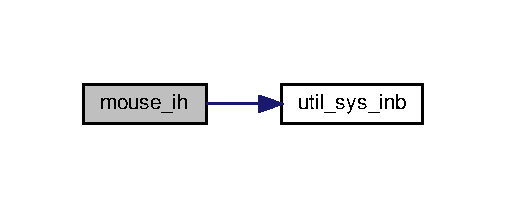
\includegraphics[width=243pt]{group__mouse_gaed4404005e4c565ac36656307386e0ac_cgraph}
\end{center}
\end{figure}
\mbox{\Hypertarget{group__mouse_gad806e677c27eae4034eeecb456323378}\label{group__mouse_gad806e677c27eae4034eeecb456323378}} 
\index{mouse@{mouse}!mouse\+\_\+ih\+\_\+disable@{mouse\+\_\+ih\+\_\+disable}}
\index{mouse\+\_\+ih\+\_\+disable@{mouse\+\_\+ih\+\_\+disable}!mouse@{mouse}}
\subsubsection{\texorpdfstring{mouse\+\_\+ih\+\_\+disable()}{mouse\_ih\_disable()}}
{\footnotesize\ttfamily int mouse\+\_\+ih\+\_\+disable (\begin{DoxyParamCaption}{ }\end{DoxyParamCaption})}



Disables mouse interrupts. 

\begin{DoxyReturn}{Returns}
0 if successful, otherwise it was not successful 
\end{DoxyReturn}
\mbox{\Hypertarget{group__mouse_ga0d1a2cd4eaf9a059b2ce3899ea8edc62}\label{group__mouse_ga0d1a2cd4eaf9a059b2ce3899ea8edc62}} 
\index{mouse@{mouse}!mouse\+\_\+ih\+\_\+enable@{mouse\+\_\+ih\+\_\+enable}}
\index{mouse\+\_\+ih\+\_\+enable@{mouse\+\_\+ih\+\_\+enable}!mouse@{mouse}}
\subsubsection{\texorpdfstring{mouse\+\_\+ih\+\_\+enable()}{mouse\_ih\_enable()}}
{\footnotesize\ttfamily int mouse\+\_\+ih\+\_\+enable (\begin{DoxyParamCaption}{ }\end{DoxyParamCaption})}



Enables mouse interrupts. 

\begin{DoxyReturn}{Returns}
0 if successful, otherwise it was not successful 
\end{DoxyReturn}
\mbox{\Hypertarget{group__mouse_ga6061042abde98af7b169c463bc203aee}\label{group__mouse_ga6061042abde98af7b169c463bc203aee}} 
\index{mouse@{mouse}!mouse\+\_\+ih\+\_\+subscribe@{mouse\+\_\+ih\+\_\+subscribe}}
\index{mouse\+\_\+ih\+\_\+subscribe@{mouse\+\_\+ih\+\_\+subscribe}!mouse@{mouse}}
\subsubsection{\texorpdfstring{mouse\+\_\+ih\+\_\+subscribe()}{mouse\_ih\_subscribe()}}
{\footnotesize\ttfamily int mouse\+\_\+ih\+\_\+subscribe (\begin{DoxyParamCaption}{ }\end{DoxyParamCaption})}



Subscribes to mouse interrupts. 

\begin{DoxyReturn}{Returns}
0 if successful, otherwise it was not successful 
\end{DoxyReturn}
\mbox{\Hypertarget{group__mouse_ga42e7f57ba1a7deeac5f9ba73bb00b80b}\label{group__mouse_ga42e7f57ba1a7deeac5f9ba73bb00b80b}} 
\index{mouse@{mouse}!mouse\+\_\+ih\+\_\+unsubscribe@{mouse\+\_\+ih\+\_\+unsubscribe}}
\index{mouse\+\_\+ih\+\_\+unsubscribe@{mouse\+\_\+ih\+\_\+unsubscribe}!mouse@{mouse}}
\subsubsection{\texorpdfstring{mouse\+\_\+ih\+\_\+unsubscribe()}{mouse\_ih\_unsubscribe()}}
{\footnotesize\ttfamily int mouse\+\_\+ih\+\_\+unsubscribe (\begin{DoxyParamCaption}{ }\end{DoxyParamCaption})}



Unsubscribes to mouse interrupts. 

\begin{DoxyReturn}{Returns}
0 if successful, otherwise it was not successful 
\end{DoxyReturn}
\mbox{\Hypertarget{group__mouse_gaf9c7f5ebd99c28946ab2184325ffa5f4}\label{group__mouse_gaf9c7f5ebd99c28946ab2184325ffa5f4}} 
\index{mouse@{mouse}!mouse\+\_\+parse\+\_\+packet@{mouse\+\_\+parse\+\_\+packet}}
\index{mouse\+\_\+parse\+\_\+packet@{mouse\+\_\+parse\+\_\+packet}!mouse@{mouse}}
\subsubsection{\texorpdfstring{mouse\+\_\+parse\+\_\+packet()}{mouse\_parse\_packet()}}
{\footnotesize\ttfamily bool mouse\+\_\+parse\+\_\+packet (\begin{DoxyParamCaption}\item[{\hyperlink{structmouse__packet}{mouse\+\_\+packet} $\ast$}]{packet }\end{DoxyParamCaption})}



The second part of mouse interrupt handling. 

Calls to this function should be preceded immediately by \hyperlink{group__mouse_gaed4404005e4c565ac36656307386e0ac}{mouse\+\_\+ih(void)}


\begin{DoxyParams}{Parameters}
{\em packet} & A \hyperlink{structmouse__packet}{mouse\+\_\+packet} pointer that will get overwritten if the packet was fully parsed \\
\hline
\end{DoxyParams}
\begin{DoxyReturn}{Returns}
true if the packet was overwritten with a new packet, otherwise false 
\end{DoxyReturn}
\mbox{\Hypertarget{group__mouse_ga8f2981a74d75d33c2e4bec9a93314711}\label{group__mouse_ga8f2981a74d75d33c2e4bec9a93314711}} 
\index{mouse@{mouse}!mouse\+\_\+send\+\_\+command@{mouse\+\_\+send\+\_\+command}}
\index{mouse\+\_\+send\+\_\+command@{mouse\+\_\+send\+\_\+command}!mouse@{mouse}}
\subsubsection{\texorpdfstring{mouse\+\_\+send\+\_\+command()}{mouse\_send\_command()}}
{\footnotesize\ttfamily int mouse\+\_\+send\+\_\+command (\begin{DoxyParamCaption}\item[{uint8\+\_\+t}]{command }\end{DoxyParamCaption})}



Sends a command to the mouse. 


\begin{DoxyParams}{Parameters}
{\em command} & The command byte to be sent \\
\hline
\end{DoxyParams}
\begin{DoxyReturn}{Returns}
0 if successful, something else otherwise 
\end{DoxyReturn}
Here is the call graph for this function\+:\nopagebreak
\begin{figure}[H]
\begin{center}
\leavevmode
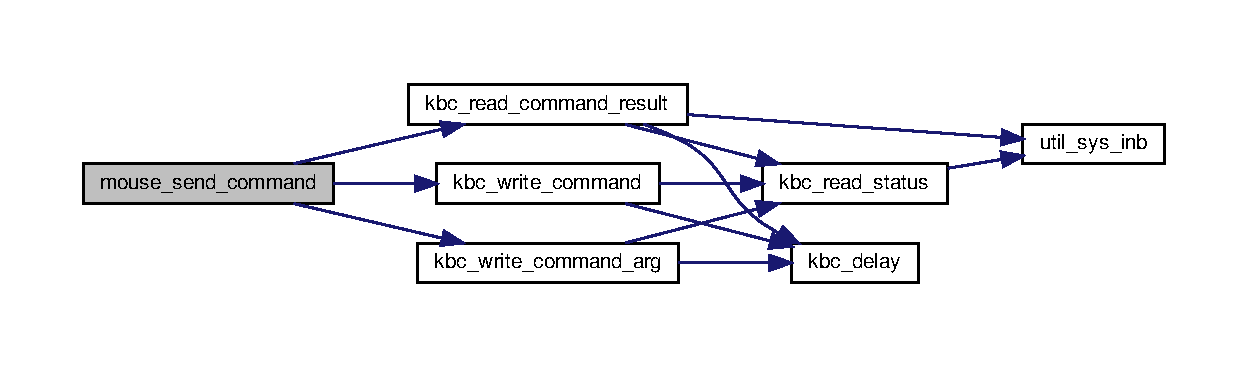
\includegraphics[width=350pt]{group__mouse_ga8f2981a74d75d33c2e4bec9a93314711_cgraph}
\end{center}
\end{figure}

\hypertarget{group__numbers}{}\section{numbers}
\label{group__numbers}\index{numbers@{numbers}}


Number drawing utilities.  


\subsection*{Macros}
\begin{DoxyCompactItemize}
\item 
\#define \hyperlink{group__numbers_ga25023eab36552ec9843c325b07ba20f8}{N\+U\+M\+B\+E\+R\+S\+\_\+\+L\+E\+N\+G\+TH}~56
\item 
\#define \hyperlink{group__numbers_ga9950e4d72e16c9672a3f936a47d2897c}{N\+U\+M\+B\+E\+R\+S\+\_\+\+H\+E\+I\+G\+HT}~32
\end{DoxyCompactItemize}
\subsection*{Functions}
\begin{DoxyCompactItemize}
\item 
void \hyperlink{group__numbers_ga957a3e5ec5d985ee4c890b5f34ac9511}{draw\+\_\+numbers} (uint8\+\_\+t $\ast$base\+\_\+ptr, uint16\+\_\+t x, uint16\+\_\+t y, uint8\+\_\+t \hyperlink{projectiles_8c_a5a648f5ec00c526b0dfa2df7a272c6c0}{n})
\begin{DoxyCompactList}\small\item\em Draws a two-\/digit number on the given buffer at the given coordinates. \end{DoxyCompactList}\end{DoxyCompactItemize}


\subsection{Detailed Description}
Number drawing utilities. 



\subsection{Macro Definition Documentation}
\mbox{\Hypertarget{group__numbers_ga9950e4d72e16c9672a3f936a47d2897c}\label{group__numbers_ga9950e4d72e16c9672a3f936a47d2897c}} 
\index{numbers@{numbers}!N\+U\+M\+B\+E\+R\+S\+\_\+\+H\+E\+I\+G\+HT@{N\+U\+M\+B\+E\+R\+S\+\_\+\+H\+E\+I\+G\+HT}}
\index{N\+U\+M\+B\+E\+R\+S\+\_\+\+H\+E\+I\+G\+HT@{N\+U\+M\+B\+E\+R\+S\+\_\+\+H\+E\+I\+G\+HT}!numbers@{numbers}}
\subsubsection{\texorpdfstring{N\+U\+M\+B\+E\+R\+S\+\_\+\+H\+E\+I\+G\+HT}{NUMBERS\_HEIGHT}}
{\footnotesize\ttfamily \#define N\+U\+M\+B\+E\+R\+S\+\_\+\+H\+E\+I\+G\+HT~32}

\mbox{\Hypertarget{group__numbers_ga25023eab36552ec9843c325b07ba20f8}\label{group__numbers_ga25023eab36552ec9843c325b07ba20f8}} 
\index{numbers@{numbers}!N\+U\+M\+B\+E\+R\+S\+\_\+\+L\+E\+N\+G\+TH@{N\+U\+M\+B\+E\+R\+S\+\_\+\+L\+E\+N\+G\+TH}}
\index{N\+U\+M\+B\+E\+R\+S\+\_\+\+L\+E\+N\+G\+TH@{N\+U\+M\+B\+E\+R\+S\+\_\+\+L\+E\+N\+G\+TH}!numbers@{numbers}}
\subsubsection{\texorpdfstring{N\+U\+M\+B\+E\+R\+S\+\_\+\+L\+E\+N\+G\+TH}{NUMBERS\_LENGTH}}
{\footnotesize\ttfamily \#define N\+U\+M\+B\+E\+R\+S\+\_\+\+L\+E\+N\+G\+TH~56}



\subsection{Function Documentation}
\mbox{\Hypertarget{group__numbers_ga957a3e5ec5d985ee4c890b5f34ac9511}\label{group__numbers_ga957a3e5ec5d985ee4c890b5f34ac9511}} 
\index{numbers@{numbers}!draw\+\_\+numbers@{draw\+\_\+numbers}}
\index{draw\+\_\+numbers@{draw\+\_\+numbers}!numbers@{numbers}}
\subsubsection{\texorpdfstring{draw\+\_\+numbers()}{draw\_numbers()}}
{\footnotesize\ttfamily void draw\+\_\+numbers (\begin{DoxyParamCaption}\item[{uint8\+\_\+t $\ast$}]{base\+\_\+ptr,  }\item[{uint16\+\_\+t}]{x,  }\item[{uint16\+\_\+t}]{y,  }\item[{uint8\+\_\+t}]{n }\end{DoxyParamCaption})}



Draws a two-\/digit number on the given buffer at the given coordinates. 


\begin{DoxyParams}{Parameters}
{\em base\+\_\+ptr} & A pointer to a buffer (must be equal in size to the frame buffer) \\
\hline
{\em x} & The x coordinate of the top left corner of the two-\/digit image (counting downwards from the top) \\
\hline
{\em y} & The y coordinate of the top left corner of the two-\/digit image (counting rightwards from the left) \\
\hline
{\em n} & The two-\/digit number \\
\hline
\end{DoxyParams}
Here is the call graph for this function\+:\nopagebreak
\begin{figure}[H]
\begin{center}
\leavevmode
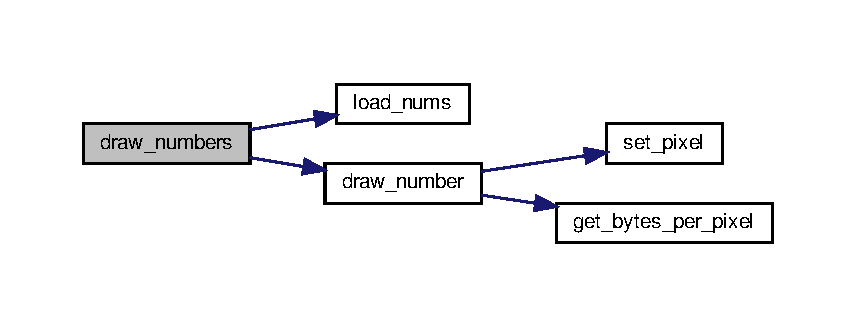
\includegraphics[width=350pt]{group__numbers_ga957a3e5ec5d985ee4c890b5f34ac9511_cgraph}
\end{center}
\end{figure}

\hypertarget{group__player}{}\section{player}
\label{group__player}\index{player@{player}}


Player-\/related functions.  


\subsection*{Data Structures}
\begin{DoxyCompactItemize}
\item 
struct \hyperlink{structplayer}{player}
\begin{DoxyCompactList}\small\item\em Struct that represents one of our game\textquotesingle{}s players. \end{DoxyCompactList}\end{DoxyCompactItemize}
\subsection*{Macros}
\begin{DoxyCompactItemize}
\item 
\#define \hyperlink{group__player_gaa6441831ca40c537df57bf5b100fe713}{L\+E\+F\+T\+\_\+\+B\+U\+T\+T\+O\+N\+\_\+M}~0x4b
\item 
\#define \hyperlink{group__player_ga9c277826f74bdfa51a6d700e375d8bd2}{R\+I\+G\+H\+T\+\_\+\+B\+U\+T\+T\+O\+N\+\_\+M}~0x4d
\item 
\#define \hyperlink{group__player_ga4c048fa9c31af5ad7cec35c5e4d0e806}{U\+P\+\_\+\+B\+U\+T\+T\+O\+N\+\_\+M}~0x48
\item 
\#define \hyperlink{group__player_ga489741c78d117de7cbc8544cec35a4de}{S\+P\+A\+C\+E\+B\+A\+R\+\_\+M}~0x39
\item 
\#define \hyperlink{group__player_ga777380ce149416afb395315a19273a7e}{L\+E\+F\+T\+\_\+\+B\+U\+T\+T\+O\+N\+\_\+B}~0xcb
\item 
\#define \hyperlink{group__player_ga6f2ca85f4bfc04c397b6102fef176a54}{R\+I\+G\+H\+T\+\_\+\+B\+U\+T\+T\+O\+N\+\_\+B}~0xcd
\item 
\#define \hyperlink{group__player_ga4f3122df972204e9abdee036dc0196fd}{U\+P\+\_\+\+B\+U\+T\+T\+O\+N\+\_\+B}~0xc8
\item 
\#define \hyperlink{group__player_gae4c8da10f184b1d26ee3797d744512b8}{S\+P\+A\+C\+E\+B\+A\+R\+\_\+B}~0xb9
\item 
\#define \hyperlink{group__player_ga57b8aa2e404b5fb79a64f44ce8c071d8}{D\+I\+S\+T\+\_\+\+F\+R\+O\+M\+\_\+\+M\+I\+D\+D\+L\+E\+\_\+\+P\+O\+I\+NT}~20
\item 
\#define \hyperlink{group__player_ga1f5d790ef3cd6eba2604b90705a1eb6b}{A\+N\+G\+L\+E\+\_\+\+O\+F\+F\+S\+ET}~2.\+5
\end{DoxyCompactItemize}
\subsection*{Typedefs}
\begin{DoxyCompactItemize}
\item 
typedef struct \hyperlink{structplayer}{player} \hyperlink{group__player_gaf40a611aff74b489090a3f7f5bedc72d}{player}
\begin{DoxyCompactList}\small\item\em Struct that represents one of our game\textquotesingle{}s players. \end{DoxyCompactList}\end{DoxyCompactItemize}
\subsection*{Functions}
\begin{DoxyCompactItemize}
\item 
void \hyperlink{group__player_gaee1b03a13fbb3fe40a1d0f4ba9c0392b}{get\+\_\+triangle} (\hyperlink{structplayer}{player} $\ast$p)
\begin{DoxyCompactList}\small\item\em It computes the player\textquotesingle{}s triangle\textquotesingle{}s vertices (\hyperlink{structplayer_ae0fa1b55cc1da566dc7bab4416193f2d}{player.\+p1x}, \hyperlink{structplayer_a7fa638c52e431ce5053b8dfcc787c778}{player.\+p1y}, \hyperlink{structplayer_a5a5d318b129ba83456be1f0a43e3e33a}{player.\+p2x}, etc.), given the player\textquotesingle{}s position and orientation. \end{DoxyCompactList}\item 
\hyperlink{structplayer}{player} $\ast$ \hyperlink{group__player_gab297abc01f8234e00c40e1a2aa9b76dd}{get\+\_\+player} (uint8\+\_\+t \hyperlink{structplayer}{player})
\item 
void \hyperlink{group__player_ga0380e53567fbcd1f4944881c14c1ea26}{update\+\_\+players\+\_\+headings} ()
\begin{DoxyCompactList}\small\item\em Updates the players\textquotesingle{} orientations with the given \hyperlink{structplayer_a54480a9ce1ccb383229691dd88d55103}{player.\+input\+\_\+direction\+\_\+delta}. \end{DoxyCompactList}\item 
void \hyperlink{group__player_gaba5c1d6b1b36aefd3412c607540f274e}{handle\+\_\+player1\+\_\+input} (\hyperlink{structkeyboard__packet}{keyboard\+\_\+packet} p1)
\begin{DoxyCompactList}\small\item\em Updates player 1\textquotesingle{}s inputs. \end{DoxyCompactList}\item 
void \hyperlink{group__player_ga34127316334c60ca280028fbaa2a4c44}{handle\+\_\+player2\+\_\+input} (\hyperlink{structmouse__packet}{mouse\+\_\+packet} p2)
\begin{DoxyCompactList}\small\item\em Updates player 2\textquotesingle{}s inputs. \end{DoxyCompactList}\item 
void \hyperlink{group__player_gae147e3272cf07f0fce5c511256eb7d04}{draw\+\_\+players} (uint8\+\_\+t $\ast$base\+\_\+ptr)
\begin{DoxyCompactList}\small\item\em Draws the players (that are alive) on the given buffer. \end{DoxyCompactList}\item 
\hyperlink{structvector2}{vector2} \hyperlink{group__player_ga42e681c6fb77fee7d6cab5a84759d796}{get\+\_\+player\+\_\+normalized\+\_\+heading} (\hyperlink{structplayer}{player} $\ast$p)
\item 
bool \hyperlink{group__player_gadc4c7fcd8773da2ab9aa8b3329753c5f}{players\+\_\+colide} ()
\item 
bool \hyperlink{group__player_ga24b1f0fee3e9f443541b9dd9ad9fe8b4}{player\+\_\+touches\+\_\+circle} (\hyperlink{structplayer}{player} $\ast$p, uint16\+\_\+t circle\+\_\+x, uint16\+\_\+t circle\+\_\+y, uint16\+\_\+t radius)
\item 
bool \hyperlink{group__player_ga431d0f0637a43f73720bb50437bba5a3}{player\+\_\+hits\+\_\+top} (\hyperlink{structplayer}{player} $\ast$p)
\item 
bool \hyperlink{group__player_ga08801e3ed5f697e05464b59448b55161}{player\+\_\+hits\+\_\+bottom} (\hyperlink{structplayer}{player} $\ast$p)
\item 
bool \hyperlink{group__player_ga48320119b999429e803eeeea71f826e6}{player\+\_\+hits\+\_\+right} (\hyperlink{structplayer}{player} $\ast$p)
\item 
bool \hyperlink{group__player_gafbba6449a23607a36fed909033f3c559}{player\+\_\+hits\+\_\+left} (\hyperlink{structplayer}{player} $\ast$p)
\end{DoxyCompactItemize}


\subsection{Detailed Description}
Player-\/related functions. 

You may be interested in how two players with different input devices (keyboard and mouse) can be represented by the same struct. We have a have an abstraction layer in the struct player (\hyperlink{structplayer_a26eb3b2626daf93d534a3504a6fc663b}{player.\+input\+\_\+accelerate} , \hyperlink{structplayer_a0ac2a27628c9f628fe4f01e522845372}{player.\+input\+\_\+shooting} and \hyperlink{structplayer_a54480a9ce1ccb383229691dd88d55103}{player.\+input\+\_\+direction\+\_\+delta}) that gets updated with different functions (\hyperlink{group__player_gaba5c1d6b1b36aefd3412c607540f274e}{handle\+\_\+player1\+\_\+input(keyboard\+\_\+packet p1)} and \hyperlink{group__player_ga34127316334c60ca280028fbaa2a4c44}{handle\+\_\+player2\+\_\+input(mouse\+\_\+packet p2)}). 

\subsection{Macro Definition Documentation}
\mbox{\Hypertarget{group__player_ga1f5d790ef3cd6eba2604b90705a1eb6b}\label{group__player_ga1f5d790ef3cd6eba2604b90705a1eb6b}} 
\index{player@{player}!A\+N\+G\+L\+E\+\_\+\+O\+F\+F\+S\+ET@{A\+N\+G\+L\+E\+\_\+\+O\+F\+F\+S\+ET}}
\index{A\+N\+G\+L\+E\+\_\+\+O\+F\+F\+S\+ET@{A\+N\+G\+L\+E\+\_\+\+O\+F\+F\+S\+ET}!player@{player}}
\subsubsection{\texorpdfstring{A\+N\+G\+L\+E\+\_\+\+O\+F\+F\+S\+ET}{ANGLE\_OFFSET}}
{\footnotesize\ttfamily \#define A\+N\+G\+L\+E\+\_\+\+O\+F\+F\+S\+ET~2.\+5}

\mbox{\Hypertarget{group__player_ga57b8aa2e404b5fb79a64f44ce8c071d8}\label{group__player_ga57b8aa2e404b5fb79a64f44ce8c071d8}} 
\index{player@{player}!D\+I\+S\+T\+\_\+\+F\+R\+O\+M\+\_\+\+M\+I\+D\+D\+L\+E\+\_\+\+P\+O\+I\+NT@{D\+I\+S\+T\+\_\+\+F\+R\+O\+M\+\_\+\+M\+I\+D\+D\+L\+E\+\_\+\+P\+O\+I\+NT}}
\index{D\+I\+S\+T\+\_\+\+F\+R\+O\+M\+\_\+\+M\+I\+D\+D\+L\+E\+\_\+\+P\+O\+I\+NT@{D\+I\+S\+T\+\_\+\+F\+R\+O\+M\+\_\+\+M\+I\+D\+D\+L\+E\+\_\+\+P\+O\+I\+NT}!player@{player}}
\subsubsection{\texorpdfstring{D\+I\+S\+T\+\_\+\+F\+R\+O\+M\+\_\+\+M\+I\+D\+D\+L\+E\+\_\+\+P\+O\+I\+NT}{DIST\_FROM\_MIDDLE\_POINT}}
{\footnotesize\ttfamily \#define D\+I\+S\+T\+\_\+\+F\+R\+O\+M\+\_\+\+M\+I\+D\+D\+L\+E\+\_\+\+P\+O\+I\+NT~20}

\mbox{\Hypertarget{group__player_ga777380ce149416afb395315a19273a7e}\label{group__player_ga777380ce149416afb395315a19273a7e}} 
\index{player@{player}!L\+E\+F\+T\+\_\+\+B\+U\+T\+T\+O\+N\+\_\+B@{L\+E\+F\+T\+\_\+\+B\+U\+T\+T\+O\+N\+\_\+B}}
\index{L\+E\+F\+T\+\_\+\+B\+U\+T\+T\+O\+N\+\_\+B@{L\+E\+F\+T\+\_\+\+B\+U\+T\+T\+O\+N\+\_\+B}!player@{player}}
\subsubsection{\texorpdfstring{L\+E\+F\+T\+\_\+\+B\+U\+T\+T\+O\+N\+\_\+B}{LEFT\_BUTTON\_B}}
{\footnotesize\ttfamily \#define L\+E\+F\+T\+\_\+\+B\+U\+T\+T\+O\+N\+\_\+B~0xcb}

\mbox{\Hypertarget{group__player_gaa6441831ca40c537df57bf5b100fe713}\label{group__player_gaa6441831ca40c537df57bf5b100fe713}} 
\index{player@{player}!L\+E\+F\+T\+\_\+\+B\+U\+T\+T\+O\+N\+\_\+M@{L\+E\+F\+T\+\_\+\+B\+U\+T\+T\+O\+N\+\_\+M}}
\index{L\+E\+F\+T\+\_\+\+B\+U\+T\+T\+O\+N\+\_\+M@{L\+E\+F\+T\+\_\+\+B\+U\+T\+T\+O\+N\+\_\+M}!player@{player}}
\subsubsection{\texorpdfstring{L\+E\+F\+T\+\_\+\+B\+U\+T\+T\+O\+N\+\_\+M}{LEFT\_BUTTON\_M}}
{\footnotesize\ttfamily \#define L\+E\+F\+T\+\_\+\+B\+U\+T\+T\+O\+N\+\_\+M~0x4b}

\mbox{\Hypertarget{group__player_ga6f2ca85f4bfc04c397b6102fef176a54}\label{group__player_ga6f2ca85f4bfc04c397b6102fef176a54}} 
\index{player@{player}!R\+I\+G\+H\+T\+\_\+\+B\+U\+T\+T\+O\+N\+\_\+B@{R\+I\+G\+H\+T\+\_\+\+B\+U\+T\+T\+O\+N\+\_\+B}}
\index{R\+I\+G\+H\+T\+\_\+\+B\+U\+T\+T\+O\+N\+\_\+B@{R\+I\+G\+H\+T\+\_\+\+B\+U\+T\+T\+O\+N\+\_\+B}!player@{player}}
\subsubsection{\texorpdfstring{R\+I\+G\+H\+T\+\_\+\+B\+U\+T\+T\+O\+N\+\_\+B}{RIGHT\_BUTTON\_B}}
{\footnotesize\ttfamily \#define R\+I\+G\+H\+T\+\_\+\+B\+U\+T\+T\+O\+N\+\_\+B~0xcd}

\mbox{\Hypertarget{group__player_ga9c277826f74bdfa51a6d700e375d8bd2}\label{group__player_ga9c277826f74bdfa51a6d700e375d8bd2}} 
\index{player@{player}!R\+I\+G\+H\+T\+\_\+\+B\+U\+T\+T\+O\+N\+\_\+M@{R\+I\+G\+H\+T\+\_\+\+B\+U\+T\+T\+O\+N\+\_\+M}}
\index{R\+I\+G\+H\+T\+\_\+\+B\+U\+T\+T\+O\+N\+\_\+M@{R\+I\+G\+H\+T\+\_\+\+B\+U\+T\+T\+O\+N\+\_\+M}!player@{player}}
\subsubsection{\texorpdfstring{R\+I\+G\+H\+T\+\_\+\+B\+U\+T\+T\+O\+N\+\_\+M}{RIGHT\_BUTTON\_M}}
{\footnotesize\ttfamily \#define R\+I\+G\+H\+T\+\_\+\+B\+U\+T\+T\+O\+N\+\_\+M~0x4d}

\mbox{\Hypertarget{group__player_gae4c8da10f184b1d26ee3797d744512b8}\label{group__player_gae4c8da10f184b1d26ee3797d744512b8}} 
\index{player@{player}!S\+P\+A\+C\+E\+B\+A\+R\+\_\+B@{S\+P\+A\+C\+E\+B\+A\+R\+\_\+B}}
\index{S\+P\+A\+C\+E\+B\+A\+R\+\_\+B@{S\+P\+A\+C\+E\+B\+A\+R\+\_\+B}!player@{player}}
\subsubsection{\texorpdfstring{S\+P\+A\+C\+E\+B\+A\+R\+\_\+B}{SPACEBAR\_B}}
{\footnotesize\ttfamily \#define S\+P\+A\+C\+E\+B\+A\+R\+\_\+B~0xb9}

\mbox{\Hypertarget{group__player_ga489741c78d117de7cbc8544cec35a4de}\label{group__player_ga489741c78d117de7cbc8544cec35a4de}} 
\index{player@{player}!S\+P\+A\+C\+E\+B\+A\+R\+\_\+M@{S\+P\+A\+C\+E\+B\+A\+R\+\_\+M}}
\index{S\+P\+A\+C\+E\+B\+A\+R\+\_\+M@{S\+P\+A\+C\+E\+B\+A\+R\+\_\+M}!player@{player}}
\subsubsection{\texorpdfstring{S\+P\+A\+C\+E\+B\+A\+R\+\_\+M}{SPACEBAR\_M}}
{\footnotesize\ttfamily \#define S\+P\+A\+C\+E\+B\+A\+R\+\_\+M~0x39}

\mbox{\Hypertarget{group__player_ga4f3122df972204e9abdee036dc0196fd}\label{group__player_ga4f3122df972204e9abdee036dc0196fd}} 
\index{player@{player}!U\+P\+\_\+\+B\+U\+T\+T\+O\+N\+\_\+B@{U\+P\+\_\+\+B\+U\+T\+T\+O\+N\+\_\+B}}
\index{U\+P\+\_\+\+B\+U\+T\+T\+O\+N\+\_\+B@{U\+P\+\_\+\+B\+U\+T\+T\+O\+N\+\_\+B}!player@{player}}
\subsubsection{\texorpdfstring{U\+P\+\_\+\+B\+U\+T\+T\+O\+N\+\_\+B}{UP\_BUTTON\_B}}
{\footnotesize\ttfamily \#define U\+P\+\_\+\+B\+U\+T\+T\+O\+N\+\_\+B~0xc8}

\mbox{\Hypertarget{group__player_ga4c048fa9c31af5ad7cec35c5e4d0e806}\label{group__player_ga4c048fa9c31af5ad7cec35c5e4d0e806}} 
\index{player@{player}!U\+P\+\_\+\+B\+U\+T\+T\+O\+N\+\_\+M@{U\+P\+\_\+\+B\+U\+T\+T\+O\+N\+\_\+M}}
\index{U\+P\+\_\+\+B\+U\+T\+T\+O\+N\+\_\+M@{U\+P\+\_\+\+B\+U\+T\+T\+O\+N\+\_\+M}!player@{player}}
\subsubsection{\texorpdfstring{U\+P\+\_\+\+B\+U\+T\+T\+O\+N\+\_\+M}{UP\_BUTTON\_M}}
{\footnotesize\ttfamily \#define U\+P\+\_\+\+B\+U\+T\+T\+O\+N\+\_\+M~0x48}



\subsection{Typedef Documentation}
\mbox{\Hypertarget{group__player_gaf40a611aff74b489090a3f7f5bedc72d}\label{group__player_gaf40a611aff74b489090a3f7f5bedc72d}} 
\index{player@{player}!player@{player}}
\index{player@{player}!player@{player}}
\subsubsection{\texorpdfstring{player}{player}}
{\footnotesize\ttfamily typedef struct \hyperlink{structplayer}{player} \hyperlink{structplayer}{player}}



Struct that represents one of our game\textquotesingle{}s players. 

The players, in our game, are represented by triangles. The reason the players\textquotesingle{} vertices are stored in the struct is because they necessary, not only for triangle drawing, but also for collision checking. Therefore, for sake of both convenience and efficiency, the players\textquotesingle{} vertices are only computed once per frame and stored in the struct itself. 

\subsection{Function Documentation}
\mbox{\Hypertarget{group__player_gae147e3272cf07f0fce5c511256eb7d04}\label{group__player_gae147e3272cf07f0fce5c511256eb7d04}} 
\index{player@{player}!draw\+\_\+players@{draw\+\_\+players}}
\index{draw\+\_\+players@{draw\+\_\+players}!player@{player}}
\subsubsection{\texorpdfstring{draw\+\_\+players()}{draw\_players()}}
{\footnotesize\ttfamily void draw\+\_\+players (\begin{DoxyParamCaption}\item[{uint8\+\_\+t $\ast$}]{base\+\_\+ptr }\end{DoxyParamCaption})}



Draws the players (that are alive) on the given buffer. 


\begin{DoxyParams}{Parameters}
{\em base\+\_\+ptr} & A pointer to a buffer (must be equal in size to the frame buffer) \\
\hline
\end{DoxyParams}
Here is the call graph for this function\+:\nopagebreak
\begin{figure}[H]
\begin{center}
\leavevmode
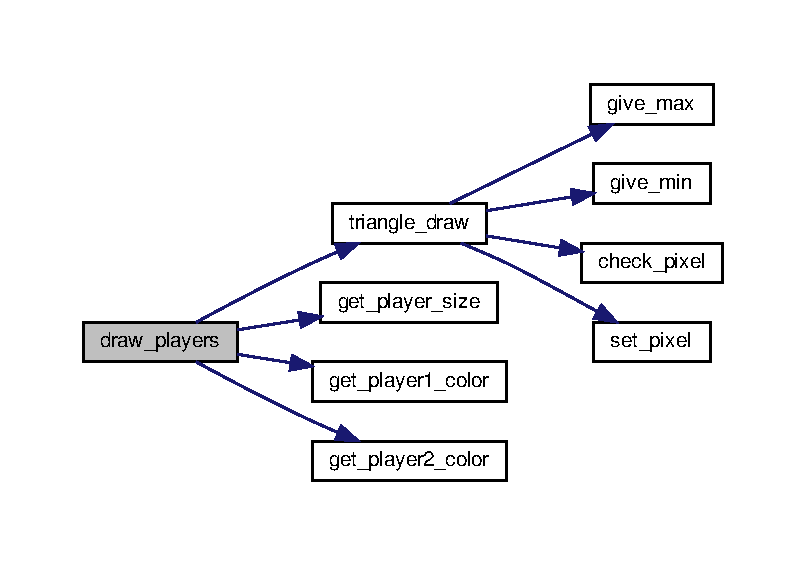
\includegraphics[width=350pt]{group__player_gae147e3272cf07f0fce5c511256eb7d04_cgraph}
\end{center}
\end{figure}
\mbox{\Hypertarget{group__player_gab297abc01f8234e00c40e1a2aa9b76dd}\label{group__player_gab297abc01f8234e00c40e1a2aa9b76dd}} 
\index{player@{player}!get\+\_\+player@{get\+\_\+player}}
\index{get\+\_\+player@{get\+\_\+player}!player@{player}}
\subsubsection{\texorpdfstring{get\+\_\+player()}{get\_player()}}
{\footnotesize\ttfamily \hyperlink{structplayer}{player}$\ast$ get\+\_\+player (\begin{DoxyParamCaption}\item[{uint8\+\_\+t}]{player }\end{DoxyParamCaption})}


\begin{DoxyParams}{Parameters}
{\em player} & The number of the player (either 1 or 2) \\
\hline
\end{DoxyParams}
\begin{DoxyReturn}{Returns}
A player pointer 
\end{DoxyReturn}
\mbox{\Hypertarget{group__player_ga42e681c6fb77fee7d6cab5a84759d796}\label{group__player_ga42e681c6fb77fee7d6cab5a84759d796}} 
\index{player@{player}!get\+\_\+player\+\_\+normalized\+\_\+heading@{get\+\_\+player\+\_\+normalized\+\_\+heading}}
\index{get\+\_\+player\+\_\+normalized\+\_\+heading@{get\+\_\+player\+\_\+normalized\+\_\+heading}!player@{player}}
\subsubsection{\texorpdfstring{get\+\_\+player\+\_\+normalized\+\_\+heading()}{get\_player\_normalized\_heading()}}
{\footnotesize\ttfamily \hyperlink{structvector2}{vector2} get\+\_\+player\+\_\+normalized\+\_\+heading (\begin{DoxyParamCaption}\item[{\hyperlink{structplayer}{player} $\ast$}]{p }\end{DoxyParamCaption})}


\begin{DoxyParams}{Parameters}
{\em p} & A pointer to a player whose heading we want \\
\hline
\end{DoxyParams}
\begin{DoxyReturn}{Returns}
The heading as a normalized \hyperlink{structvector2}{vector2} 
\end{DoxyReturn}
\mbox{\Hypertarget{group__player_gaee1b03a13fbb3fe40a1d0f4ba9c0392b}\label{group__player_gaee1b03a13fbb3fe40a1d0f4ba9c0392b}} 
\index{player@{player}!get\+\_\+triangle@{get\+\_\+triangle}}
\index{get\+\_\+triangle@{get\+\_\+triangle}!player@{player}}
\subsubsection{\texorpdfstring{get\+\_\+triangle()}{get\_triangle()}}
{\footnotesize\ttfamily void get\+\_\+triangle (\begin{DoxyParamCaption}\item[{\hyperlink{structplayer}{player} $\ast$}]{p }\end{DoxyParamCaption})}



It computes the player\textquotesingle{}s triangle\textquotesingle{}s vertices (\hyperlink{structplayer_ae0fa1b55cc1da566dc7bab4416193f2d}{player.\+p1x}, \hyperlink{structplayer_a7fa638c52e431ce5053b8dfcc787c778}{player.\+p1y}, \hyperlink{structplayer_a5a5d318b129ba83456be1f0a43e3e33a}{player.\+p2x}, etc.), given the player\textquotesingle{}s position and orientation. 


\begin{DoxyParams}{Parameters}
{\em p} & A pointer to he player whose vertices are going to get updated \\
\hline
\end{DoxyParams}
Here is the call graph for this function\+:\nopagebreak
\begin{figure}[H]
\begin{center}
\leavevmode
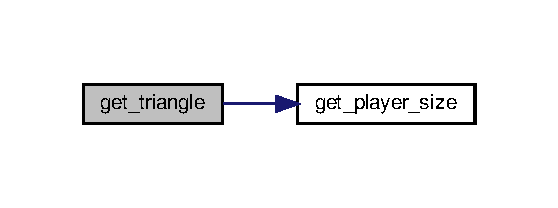
\includegraphics[width=268pt]{group__player_gaee1b03a13fbb3fe40a1d0f4ba9c0392b_cgraph}
\end{center}
\end{figure}
\mbox{\Hypertarget{group__player_gaba5c1d6b1b36aefd3412c607540f274e}\label{group__player_gaba5c1d6b1b36aefd3412c607540f274e}} 
\index{player@{player}!handle\+\_\+player1\+\_\+input@{handle\+\_\+player1\+\_\+input}}
\index{handle\+\_\+player1\+\_\+input@{handle\+\_\+player1\+\_\+input}!player@{player}}
\subsubsection{\texorpdfstring{handle\+\_\+player1\+\_\+input()}{handle\_player1\_input()}}
{\footnotesize\ttfamily void handle\+\_\+player1\+\_\+input (\begin{DoxyParamCaption}\item[{\hyperlink{structkeyboard__packet}{keyboard\+\_\+packet}}]{p1 }\end{DoxyParamCaption})}



Updates player 1\textquotesingle{}s inputs. 


\begin{DoxyParams}{Parameters}
{\em p1} & The keyboard packet \\
\hline
\end{DoxyParams}
\mbox{\Hypertarget{group__player_ga34127316334c60ca280028fbaa2a4c44}\label{group__player_ga34127316334c60ca280028fbaa2a4c44}} 
\index{player@{player}!handle\+\_\+player2\+\_\+input@{handle\+\_\+player2\+\_\+input}}
\index{handle\+\_\+player2\+\_\+input@{handle\+\_\+player2\+\_\+input}!player@{player}}
\subsubsection{\texorpdfstring{handle\+\_\+player2\+\_\+input()}{handle\_player2\_input()}}
{\footnotesize\ttfamily void handle\+\_\+player2\+\_\+input (\begin{DoxyParamCaption}\item[{\hyperlink{structmouse__packet}{mouse\+\_\+packet}}]{p2 }\end{DoxyParamCaption})}



Updates player 2\textquotesingle{}s inputs. 


\begin{DoxyParams}{Parameters}
{\em p2} & The mouse packet \\
\hline
\end{DoxyParams}
\mbox{\Hypertarget{group__player_ga08801e3ed5f697e05464b59448b55161}\label{group__player_ga08801e3ed5f697e05464b59448b55161}} 
\index{player@{player}!player\+\_\+hits\+\_\+bottom@{player\+\_\+hits\+\_\+bottom}}
\index{player\+\_\+hits\+\_\+bottom@{player\+\_\+hits\+\_\+bottom}!player@{player}}
\subsubsection{\texorpdfstring{player\+\_\+hits\+\_\+bottom()}{player\_hits\_bottom()}}
{\footnotesize\ttfamily bool player\+\_\+hits\+\_\+bottom (\begin{DoxyParamCaption}\item[{\hyperlink{structplayer}{player} $\ast$}]{p }\end{DoxyParamCaption})}


\begin{DoxyParams}{Parameters}
{\em p} & A pointer to the player we want to check \\
\hline
\end{DoxyParams}
\begin{DoxyReturn}{Returns}
true if the player is hitting the bottom of the screen, otherwise false 
\end{DoxyReturn}
Here is the call graph for this function\+:\nopagebreak
\begin{figure}[H]
\begin{center}
\leavevmode
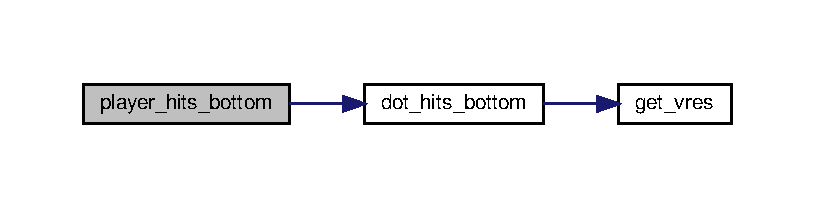
\includegraphics[width=350pt]{group__player_ga08801e3ed5f697e05464b59448b55161_cgraph}
\end{center}
\end{figure}
\mbox{\Hypertarget{group__player_gafbba6449a23607a36fed909033f3c559}\label{group__player_gafbba6449a23607a36fed909033f3c559}} 
\index{player@{player}!player\+\_\+hits\+\_\+left@{player\+\_\+hits\+\_\+left}}
\index{player\+\_\+hits\+\_\+left@{player\+\_\+hits\+\_\+left}!player@{player}}
\subsubsection{\texorpdfstring{player\+\_\+hits\+\_\+left()}{player\_hits\_left()}}
{\footnotesize\ttfamily bool player\+\_\+hits\+\_\+left (\begin{DoxyParamCaption}\item[{\hyperlink{structplayer}{player} $\ast$}]{p }\end{DoxyParamCaption})}


\begin{DoxyParams}{Parameters}
{\em p} & A pointer to the player we want to check \\
\hline
\end{DoxyParams}
\begin{DoxyReturn}{Returns}
true if the player is hitting the left of the screen, otherwise false 
\end{DoxyReturn}
Here is the call graph for this function\+:\nopagebreak
\begin{figure}[H]
\begin{center}
\leavevmode
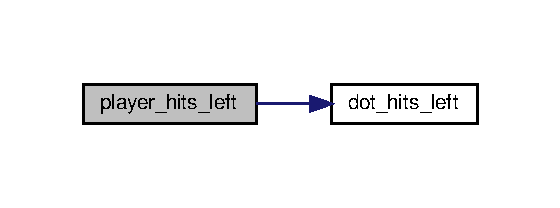
\includegraphics[width=269pt]{group__player_gafbba6449a23607a36fed909033f3c559_cgraph}
\end{center}
\end{figure}
\mbox{\Hypertarget{group__player_ga48320119b999429e803eeeea71f826e6}\label{group__player_ga48320119b999429e803eeeea71f826e6}} 
\index{player@{player}!player\+\_\+hits\+\_\+right@{player\+\_\+hits\+\_\+right}}
\index{player\+\_\+hits\+\_\+right@{player\+\_\+hits\+\_\+right}!player@{player}}
\subsubsection{\texorpdfstring{player\+\_\+hits\+\_\+right()}{player\_hits\_right()}}
{\footnotesize\ttfamily bool player\+\_\+hits\+\_\+right (\begin{DoxyParamCaption}\item[{\hyperlink{structplayer}{player} $\ast$}]{p }\end{DoxyParamCaption})}


\begin{DoxyParams}{Parameters}
{\em p} & A pointer to the player we want to check \\
\hline
\end{DoxyParams}
\begin{DoxyReturn}{Returns}
true if the player is hitting the right of the screen, otherwise false 
\end{DoxyReturn}
Here is the call graph for this function\+:\nopagebreak
\begin{figure}[H]
\begin{center}
\leavevmode
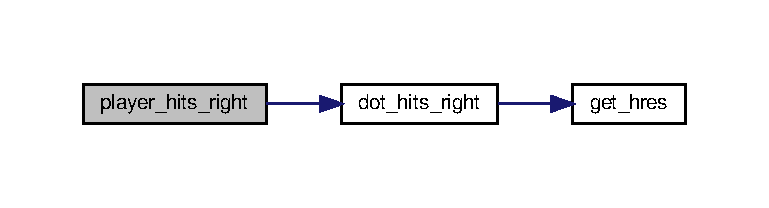
\includegraphics[width=350pt]{group__player_ga48320119b999429e803eeeea71f826e6_cgraph}
\end{center}
\end{figure}
\mbox{\Hypertarget{group__player_ga431d0f0637a43f73720bb50437bba5a3}\label{group__player_ga431d0f0637a43f73720bb50437bba5a3}} 
\index{player@{player}!player\+\_\+hits\+\_\+top@{player\+\_\+hits\+\_\+top}}
\index{player\+\_\+hits\+\_\+top@{player\+\_\+hits\+\_\+top}!player@{player}}
\subsubsection{\texorpdfstring{player\+\_\+hits\+\_\+top()}{player\_hits\_top()}}
{\footnotesize\ttfamily bool player\+\_\+hits\+\_\+top (\begin{DoxyParamCaption}\item[{\hyperlink{structplayer}{player} $\ast$}]{p }\end{DoxyParamCaption})}


\begin{DoxyParams}{Parameters}
{\em p} & A pointer to the player we want to check \\
\hline
\end{DoxyParams}
\begin{DoxyReturn}{Returns}
true if the player is hitting the top of the screen, otherwise false 
\end{DoxyReturn}
Here is the call graph for this function\+:\nopagebreak
\begin{figure}[H]
\begin{center}
\leavevmode
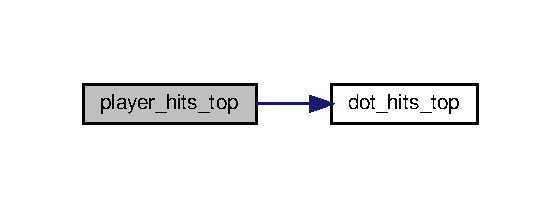
\includegraphics[width=269pt]{group__player_ga431d0f0637a43f73720bb50437bba5a3_cgraph}
\end{center}
\end{figure}
\mbox{\Hypertarget{group__player_ga24b1f0fee3e9f443541b9dd9ad9fe8b4}\label{group__player_ga24b1f0fee3e9f443541b9dd9ad9fe8b4}} 
\index{player@{player}!player\+\_\+touches\+\_\+circle@{player\+\_\+touches\+\_\+circle}}
\index{player\+\_\+touches\+\_\+circle@{player\+\_\+touches\+\_\+circle}!player@{player}}
\subsubsection{\texorpdfstring{player\+\_\+touches\+\_\+circle()}{player\_touches\_circle()}}
{\footnotesize\ttfamily bool player\+\_\+touches\+\_\+circle (\begin{DoxyParamCaption}\item[{\hyperlink{structplayer}{player} $\ast$}]{p,  }\item[{uint16\+\_\+t}]{circle\+\_\+x,  }\item[{uint16\+\_\+t}]{circle\+\_\+y,  }\item[{uint16\+\_\+t}]{radius }\end{DoxyParamCaption})}


\begin{DoxyParams}{Parameters}
{\em p} & A pointer to the player we want to check \\
\hline
{\em circle\+\_\+x} & The x coordinate of the circle \\
\hline
{\em circle\+\_\+y} & The y coordinate of the circle \\
\hline
{\em radius} & The radius of the circle \\
\hline
\end{DoxyParams}
\begin{DoxyReturn}{Returns}
true if the player is touching the circle, otherwise false 
\end{DoxyReturn}
Here is the call graph for this function\+:\nopagebreak
\begin{figure}[H]
\begin{center}
\leavevmode
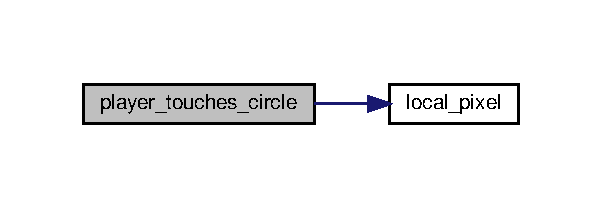
\includegraphics[width=289pt]{group__player_ga24b1f0fee3e9f443541b9dd9ad9fe8b4_cgraph}
\end{center}
\end{figure}
\mbox{\Hypertarget{group__player_gadc4c7fcd8773da2ab9aa8b3329753c5f}\label{group__player_gadc4c7fcd8773da2ab9aa8b3329753c5f}} 
\index{player@{player}!players\+\_\+colide@{players\+\_\+colide}}
\index{players\+\_\+colide@{players\+\_\+colide}!player@{player}}
\subsubsection{\texorpdfstring{players\+\_\+colide()}{players\_colide()}}
{\footnotesize\ttfamily bool players\+\_\+colide (\begin{DoxyParamCaption}{ }\end{DoxyParamCaption})}

\begin{DoxyReturn}{Returns}
true if the players are touching each other, otherwise false 
\end{DoxyReturn}
Here is the call graph for this function\+:\nopagebreak
\begin{figure}[H]
\begin{center}
\leavevmode
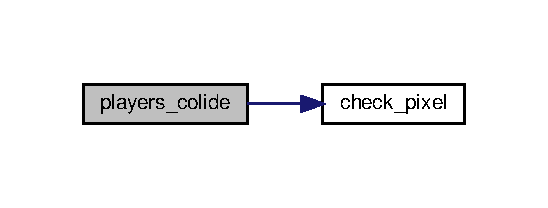
\includegraphics[width=263pt]{group__player_gadc4c7fcd8773da2ab9aa8b3329753c5f_cgraph}
\end{center}
\end{figure}
\mbox{\Hypertarget{group__player_ga0380e53567fbcd1f4944881c14c1ea26}\label{group__player_ga0380e53567fbcd1f4944881c14c1ea26}} 
\index{player@{player}!update\+\_\+players\+\_\+headings@{update\+\_\+players\+\_\+headings}}
\index{update\+\_\+players\+\_\+headings@{update\+\_\+players\+\_\+headings}!player@{player}}
\subsubsection{\texorpdfstring{update\+\_\+players\+\_\+headings()}{update\_players\_headings()}}
{\footnotesize\ttfamily void update\+\_\+players\+\_\+headings (\begin{DoxyParamCaption}{ }\end{DoxyParamCaption})}



Updates the players\textquotesingle{} orientations with the given \hyperlink{structplayer_a54480a9ce1ccb383229691dd88d55103}{player.\+input\+\_\+direction\+\_\+delta}. 


\hypertarget{group__projectiles}{}\section{projectiles}
\label{group__projectiles}\index{projectiles@{projectiles}}


projectile-\/related functions  


\subsection*{Data Structures}
\begin{DoxyCompactItemize}
\item 
struct \hyperlink{structprojectile}{projectile}
\begin{DoxyCompactList}\small\item\em Struct that represents one of our game\textquotesingle{}s bullets. \end{DoxyCompactList}\end{DoxyCompactItemize}
\subsection*{Typedefs}
\begin{DoxyCompactItemize}
\item 
typedef struct \hyperlink{structprojectile}{projectile} \hyperlink{group__projectiles_ga0ecdecffd31e7e21a2db68fb1aef8f23}{projectile}
\begin{DoxyCompactList}\small\item\em Struct that represents one of our game\textquotesingle{}s bullets. \end{DoxyCompactList}\end{DoxyCompactItemize}
\subsection*{Functions}
\begin{DoxyCompactItemize}
\item 
uint8\+\_\+t \hyperlink{group__projectiles_ga5694db4d07322ea0cb9792dd0409dcd6}{get\+\_\+n\+\_\+projectiles} ()
\item 
\hyperlink{structprojectile}{projectile} $\ast$ \hyperlink{group__projectiles_ga83c71feca8610bd78396e078b96c7607}{get\+\_\+proj\+\_\+array} ()
\item 
void \hyperlink{group__projectiles_ga1b3d00bd49fc0770838c70cb1d2d9e94}{projectile\+\_\+alloc} (uint8\+\_\+t \hyperlink{projectiles_8c_a72f6a4ef5d831709c1c10ff632d608ec}{n\+\_\+projectiles})
\item 
void \hyperlink{group__projectiles_ga1dcccbbcaf5fbc336ec52666ff0960ac}{new\+\_\+projectile} (\hyperlink{structvector2}{vector2} pos, \hyperlink{structvector2}{vector2} speed)
\begin{DoxyCompactList}\small\item\em Spawns a new projectile with the given position and velocity. \end{DoxyCompactList}\item 
void \hyperlink{group__projectiles_gae77390eb18c5b9c31165e891a1ab4b19}{draw\+\_\+projectiles} (uint8\+\_\+t $\ast$base\+\_\+ptr)
\begin{DoxyCompactList}\small\item\em Draws the projectiles on the given buffer. \end{DoxyCompactList}\end{DoxyCompactItemize}


\subsection{Detailed Description}
projectile-\/related functions 

The bullets that you see on screen while playing are allocated here (when you call \hyperlink{group__projectiles_ga1b3d00bd49fc0770838c70cb1d2d9e94}{projectile\+\_\+alloc(uint8\+\_\+t n\+\_\+projectiles)}) as an array of n\+\_\+projectiles elements. This array is, in the context of this module, a circular buffer. When projectile\+\_\+alloc is called, all the projectiles are initialized with the atribute \char`\"{}active\char`\"{} set as false. As the function new\+\_\+projectile is called, the \char`\"{}active\char`\"{} atribute of more and more elements get set to true. When you want to \char`\"{}delete\char`\"{} a projectile, you simply set that projectile\textquotesingle{}s \char`\"{}active\char`\"{} attribute to false. 

\subsection{Typedef Documentation}
\mbox{\Hypertarget{group__projectiles_ga0ecdecffd31e7e21a2db68fb1aef8f23}\label{group__projectiles_ga0ecdecffd31e7e21a2db68fb1aef8f23}} 
\index{projectiles@{projectiles}!projectile@{projectile}}
\index{projectile@{projectile}!projectiles@{projectiles}}
\subsubsection{\texorpdfstring{projectile}{projectile}}
{\footnotesize\ttfamily typedef struct \hyperlink{structprojectile}{projectile}  \hyperlink{structprojectile}{projectile}}



Struct that represents one of our game\textquotesingle{}s bullets. 



\subsection{Function Documentation}
\mbox{\Hypertarget{group__projectiles_gae77390eb18c5b9c31165e891a1ab4b19}\label{group__projectiles_gae77390eb18c5b9c31165e891a1ab4b19}} 
\index{projectiles@{projectiles}!draw\+\_\+projectiles@{draw\+\_\+projectiles}}
\index{draw\+\_\+projectiles@{draw\+\_\+projectiles}!projectiles@{projectiles}}
\subsubsection{\texorpdfstring{draw\+\_\+projectiles()}{draw\_projectiles()}}
{\footnotesize\ttfamily void draw\+\_\+projectiles (\begin{DoxyParamCaption}\item[{uint8\+\_\+t $\ast$}]{base\+\_\+ptr }\end{DoxyParamCaption})}



Draws the projectiles on the given buffer. 


\begin{DoxyParams}{Parameters}
{\em base\+\_\+ptr} & A pointer to a buffer (must be equal in size to the frame buffer) \\
\hline
\end{DoxyParams}
Here is the call graph for this function\+:\nopagebreak
\begin{figure}[H]
\begin{center}
\leavevmode
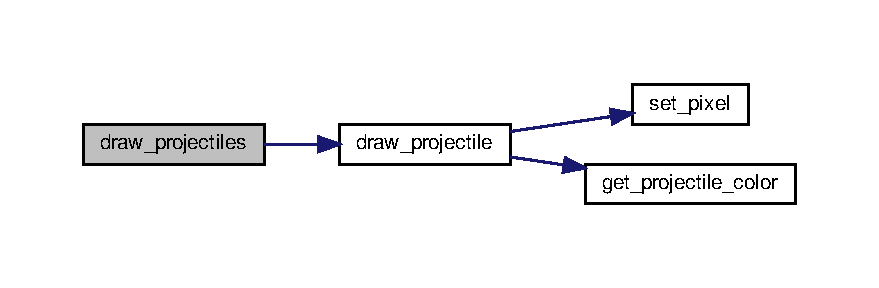
\includegraphics[width=350pt]{group__projectiles_gae77390eb18c5b9c31165e891a1ab4b19_cgraph}
\end{center}
\end{figure}
\mbox{\Hypertarget{group__projectiles_ga5694db4d07322ea0cb9792dd0409dcd6}\label{group__projectiles_ga5694db4d07322ea0cb9792dd0409dcd6}} 
\index{projectiles@{projectiles}!get\+\_\+n\+\_\+projectiles@{get\+\_\+n\+\_\+projectiles}}
\index{get\+\_\+n\+\_\+projectiles@{get\+\_\+n\+\_\+projectiles}!projectiles@{projectiles}}
\subsubsection{\texorpdfstring{get\+\_\+n\+\_\+projectiles()}{get\_n\_projectiles()}}
{\footnotesize\ttfamily uint8\+\_\+t get\+\_\+n\+\_\+projectiles (\begin{DoxyParamCaption}{ }\end{DoxyParamCaption})}

\begin{DoxyReturn}{Returns}
The size of the projectile array 
\end{DoxyReturn}
\mbox{\Hypertarget{group__projectiles_ga83c71feca8610bd78396e078b96c7607}\label{group__projectiles_ga83c71feca8610bd78396e078b96c7607}} 
\index{projectiles@{projectiles}!get\+\_\+proj\+\_\+array@{get\+\_\+proj\+\_\+array}}
\index{get\+\_\+proj\+\_\+array@{get\+\_\+proj\+\_\+array}!projectiles@{projectiles}}
\subsubsection{\texorpdfstring{get\+\_\+proj\+\_\+array()}{get\_proj\_array()}}
{\footnotesize\ttfamily \hyperlink{structprojectile}{projectile}$\ast$ get\+\_\+proj\+\_\+array (\begin{DoxyParamCaption}{ }\end{DoxyParamCaption})}

\begin{DoxyReturn}{Returns}
A pointer to the beginning of the projectile array 
\end{DoxyReturn}
\mbox{\Hypertarget{group__projectiles_ga1dcccbbcaf5fbc336ec52666ff0960ac}\label{group__projectiles_ga1dcccbbcaf5fbc336ec52666ff0960ac}} 
\index{projectiles@{projectiles}!new\+\_\+projectile@{new\+\_\+projectile}}
\index{new\+\_\+projectile@{new\+\_\+projectile}!projectiles@{projectiles}}
\subsubsection{\texorpdfstring{new\+\_\+projectile()}{new\_projectile()}}
{\footnotesize\ttfamily void new\+\_\+projectile (\begin{DoxyParamCaption}\item[{\hyperlink{structvector2}{vector2}}]{pos,  }\item[{\hyperlink{structvector2}{vector2}}]{speed }\end{DoxyParamCaption})}



Spawns a new projectile with the given position and velocity. 

It overwrites a projectile in buffer with the new position and speed, and sets \char`\"{}active\char`\"{} to true


\begin{DoxyParams}{Parameters}
{\em pos} & The position of the new projectile \\
\hline
{\em speed} & The speed of the new projectile \\
\hline
\end{DoxyParams}
\mbox{\Hypertarget{group__projectiles_ga1b3d00bd49fc0770838c70cb1d2d9e94}\label{group__projectiles_ga1b3d00bd49fc0770838c70cb1d2d9e94}} 
\index{projectiles@{projectiles}!projectile\+\_\+alloc@{projectile\+\_\+alloc}}
\index{projectile\+\_\+alloc@{projectile\+\_\+alloc}!projectiles@{projectiles}}
\subsubsection{\texorpdfstring{projectile\+\_\+alloc()}{projectile\_alloc()}}
{\footnotesize\ttfamily void projectile\+\_\+alloc (\begin{DoxyParamCaption}\item[{uint8\+\_\+t}]{n\+\_\+projectiles }\end{DoxyParamCaption})}

\begin{DoxyReturn}{Returns}
A pointer to the beginning of the projectile array 
\end{DoxyReturn}

\hypertarget{group__rtc}{}\section{rtc}
\label{group__rtc}\index{rtc@{rtc}}


R\+T\+C-\/related interrupt and register-\/reading/writing functions.  


\subsection*{Macros}
\begin{DoxyCompactItemize}
\item 
\#define \hyperlink{group__rtc_ga4e22feb6ffbc1cda32fadff5c740dc51}{R\+T\+C\+\_\+\+I\+RQ}~8
\item 
\#define \hyperlink{group__rtc_gac93f7885d306a82906ee65bdbf0db65d}{R\+T\+C\+\_\+\+H\+O\+O\+K\+\_\+\+ID}~3
\item 
\#define \hyperlink{group__rtc_gab54f2d18b47b47a59f718e16099446e8}{R\+T\+C\+\_\+\+M\+A\+SK}~B\+IT(\hyperlink{group__rtc_gac93f7885d306a82906ee65bdbf0db65d}{R\+T\+C\+\_\+\+H\+O\+O\+K\+\_\+\+ID})
\item 
\#define \hyperlink{group__rtc_ga43f6540c6d3a78b930f9adad56cf7fac}{R\+T\+C\+\_\+\+S\+E\+C\+O\+N\+DS}~0
\item 
\#define \hyperlink{group__rtc_gaba1a00fd8dcaa066bbb9cecacb4dd04b}{R\+T\+C\+\_\+\+S\+E\+C\+O\+N\+D\+S\+\_\+\+A\+L\+A\+RM}~1
\item 
\#define \hyperlink{group__rtc_gaabc0725ac27ea93c913a2a4d7cd51ac7}{R\+T\+C\+\_\+\+M\+I\+N\+U\+T\+ES}~2
\item 
\#define \hyperlink{group__rtc_ga3354ceb0b3dc74b2ff1123ecd0b7c043}{R\+T\+C\+\_\+\+M\+I\+N\+U\+T\+E\+S\+\_\+\+A\+L\+A\+RM}~3
\item 
\#define \hyperlink{group__rtc_ga4d74cdb9a956c4f1783ad5aff00dc2b8}{R\+T\+C\+\_\+\+H\+O\+U\+RS}~4
\item 
\#define \hyperlink{group__rtc_ga736eabe8fe923b38d85437697f37ba35}{R\+T\+C\+\_\+\+H\+O\+U\+R\+S\+\_\+\+A\+L\+A\+RM}~5
\item 
\#define \hyperlink{group__rtc_ga7ed5faace1f720b524bfb2ef119a7123}{R\+T\+C\+\_\+\+D\+A\+Y\+\_\+\+O\+F\+\_\+\+T\+H\+E\+\_\+\+W\+E\+EK}~6
\item 
\#define \hyperlink{group__rtc_ga8d7ce94679a93c7844b73de578abb9c9}{R\+T\+C\+\_\+\+D\+A\+Y\+\_\+\+O\+F\+\_\+\+T\+H\+E\+\_\+\+M\+O\+N\+TH}~7
\item 
\#define \hyperlink{group__rtc_gabda0c877ee1a02b8351c0cfe72838088}{R\+T\+C\+\_\+\+M\+O\+N\+TH}~8
\item 
\#define \hyperlink{group__rtc_ga1df5568e6774b73aa4c6e59fc40e9147}{R\+T\+C\+\_\+\+Y\+E\+AR}~9
\item 
\#define \hyperlink{group__rtc_ga81f35849e2c8fe00b1e66b085db986fa}{R\+T\+C\+\_\+\+R\+E\+G\+I\+S\+T\+E\+R\+\_\+A}~10
\item 
\#define \hyperlink{group__rtc_gaa7c10a34d778f2e5bc0f8867ba205f0d}{R\+T\+C\+\_\+\+R\+E\+G\+I\+S\+T\+E\+R\+\_\+B}~11
\item 
\#define \hyperlink{group__rtc_gac1a40b5e35c16b2467bcb5c09a6c1125}{R\+T\+C\+\_\+\+R\+E\+G\+I\+S\+T\+E\+R\+\_\+C}~12
\item 
\#define \hyperlink{group__rtc_ga49ae921cc8c2c61cbbd0b0e779e50057}{R\+T\+C\+\_\+\+R\+E\+G\+I\+S\+T\+E\+R\+\_\+D}~13
\item 
\#define \hyperlink{group__rtc_ga710b98232df2c563009e6f8a6cd18220}{R\+T\+C\+\_\+\+A\+D\+D\+R\+\_\+\+R\+EG}~0x70
\item 
\#define \hyperlink{group__rtc_ga2f258a00c59c3f347c8d2d4a75471ce0}{R\+T\+C\+\_\+\+D\+A\+T\+A\+\_\+\+R\+EG}~0x71
\item 
\#define \hyperlink{group__rtc_ga2d0dea617451446330a89387a9dfed99}{R\+T\+C\+\_\+\+R\+E\+G\+\_\+\+A\+\_\+\+U\+IP}~B\+IT(7)
\item 
\#define \hyperlink{group__rtc_ga0f56a2e4d35b0ad99f8fe85b425f59dc}{R\+T\+C\+\_\+\+R\+E\+G\+\_\+\+B\+\_\+\+S\+ET}~B\+IT(7)
\item 
\#define \hyperlink{group__rtc_ga7a275b39d2b9880655bf653b953b425e}{R\+T\+C\+\_\+\+R\+E\+G\+\_\+\+B\+\_\+\+P\+IE}~B\+IT(6)
\item 
\#define \hyperlink{group__rtc_ga4966ec0df7137606da48c11e339173a8}{R\+T\+C\+\_\+\+R\+E\+G\+\_\+\+B\+\_\+\+A\+IE}~B\+IT(5)
\item 
\#define \hyperlink{group__rtc_gac49ad037dea0a2eac11860a6c01a05a2}{R\+T\+C\+\_\+\+R\+E\+G\+\_\+\+B\+\_\+\+U\+IE}~B\+IT(4)
\item 
\#define \hyperlink{group__rtc_gabc5526120e6a1f035ef362b6f4fa5b63}{R\+T\+C\+\_\+\+R\+E\+G\+\_\+\+B\+\_\+\+S\+Q\+WE}~B\+IT(3)
\item 
\#define \hyperlink{group__rtc_ga9dc43c3d09d5ff86a6ccc538c922de85}{R\+T\+C\+\_\+\+R\+E\+G\+\_\+\+B\+\_\+\+DM}~B\+IT(2)
\item 
\#define \hyperlink{group__rtc_ga5009d8d9738bc5c2a0e1ffcf5845e132}{R\+T\+C\+\_\+\+R\+E\+G\+\_\+\+B\+\_\+24\+\_\+12}~B\+IT(1)
\item 
\#define \hyperlink{group__rtc_ga1fc0acfa01a11ca65cf1e472f4a49e99}{R\+T\+C\+\_\+\+R\+E\+G\+\_\+\+B\+\_\+\+D\+SE}~B\+IT(0)
\item 
\#define \hyperlink{group__rtc_ga38174f5b51b268ab91bc0d9e4f9177c8}{R\+T\+C\+\_\+\+R\+E\+G\+\_\+\+C\+\_\+\+I\+R\+QF}~B\+IT(7)
\item 
\#define \hyperlink{group__rtc_ga4e96da8e6998c6a7b275d8d1d2e21657}{R\+T\+C\+\_\+\+R\+E\+G\+\_\+\+C\+\_\+\+PF}~B\+IT(6)
\item 
\#define \hyperlink{group__rtc_ga5d87d84ef1cc2472d66bea9f1309cd60}{R\+T\+C\+\_\+\+R\+E\+G\+\_\+\+C\+\_\+\+AF}~B\+IT(5)
\item 
\#define \hyperlink{group__rtc_gaf8ce7b20a854a0ce90b2954cc1cef920}{R\+T\+C\+\_\+\+R\+E\+G\+\_\+\+C\+\_\+\+UF}~B\+IT(4)
\end{DoxyCompactItemize}
\subsection*{Functions}
\begin{DoxyCompactItemize}
\item 
bool \hyperlink{group__rtc_ga55d98e39c0c2bf246ef774491c31b593}{rtc\+\_\+ih} ()
\begin{DoxyCompactList}\small\item\em Handles R\+TC interrupts. \end{DoxyCompactList}\item 
int \hyperlink{group__rtc_gaa9a633f60d6ee3b237a80b408647908c}{rtc\+\_\+ih\+\_\+subscribe} ()
\begin{DoxyCompactList}\small\item\em Subscribes to R\+TC interrupts. \end{DoxyCompactList}\item 
int \hyperlink{group__rtc_ga9c629cc80f25b7d9d4e19fb6f6de8ea4}{rtc\+\_\+ih\+\_\+unsubscribe} ()
\begin{DoxyCompactList}\small\item\em Unsubscribes to R\+TC interrupts. \end{DoxyCompactList}\item 
int \hyperlink{group__rtc_ga272e00608ea1e5f0e931ae7a566c2af4}{rtc\+\_\+ih\+\_\+enable} ()
\begin{DoxyCompactList}\small\item\em Enables R\+TC interrupts. \end{DoxyCompactList}\item 
int \hyperlink{group__rtc_gaacd5a961df48ee02b0d95588cbe00be5}{rtc\+\_\+ih\+\_\+disable} ()
\begin{DoxyCompactList}\small\item\em Disables R\+TC interrupts. \end{DoxyCompactList}\item 
void \hyperlink{group__rtc_ga9d32737436e666dcd33816dd240321a8}{rtc\+\_\+write\+\_\+reg} (uint8\+\_\+t reg, uint8\+\_\+t data)
\begin{DoxyCompactList}\small\item\em Writes the R\+TC register at position reg. \end{DoxyCompactList}\item 
uint8\+\_\+t \hyperlink{group__rtc_ga967406c372c2ba0b6b18c4784d5b1ce2}{rtc\+\_\+read\+\_\+reg} (uint8\+\_\+t reg)
\begin{DoxyCompactList}\small\item\em Reads the R\+TC register at position reg. \end{DoxyCompactList}\item 
uint8\+\_\+t \hyperlink{group__rtc_ga94b0c84824555e206801ea5a59eaa8fb}{rtc\+\_\+get\+\_\+hour} ()
\item 
uint8\+\_\+t \hyperlink{group__rtc_ga045f10751f73dcf26ec496d24332e067}{rtc\+\_\+get\+\_\+minute} ()
\item 
uint8\+\_\+t \hyperlink{group__rtc_ga900a6f54c5751abfa35460384278ec84}{rtc\+\_\+get\+\_\+second} ()
\end{DoxyCompactItemize}


\subsection{Detailed Description}
R\+T\+C-\/related interrupt and register-\/reading/writing functions. 



\subsection{Macro Definition Documentation}
\mbox{\Hypertarget{group__rtc_ga710b98232df2c563009e6f8a6cd18220}\label{group__rtc_ga710b98232df2c563009e6f8a6cd18220}} 
\index{rtc@{rtc}!R\+T\+C\+\_\+\+A\+D\+D\+R\+\_\+\+R\+EG@{R\+T\+C\+\_\+\+A\+D\+D\+R\+\_\+\+R\+EG}}
\index{R\+T\+C\+\_\+\+A\+D\+D\+R\+\_\+\+R\+EG@{R\+T\+C\+\_\+\+A\+D\+D\+R\+\_\+\+R\+EG}!rtc@{rtc}}
\subsubsection{\texorpdfstring{R\+T\+C\+\_\+\+A\+D\+D\+R\+\_\+\+R\+EG}{RTC\_ADDR\_REG}}
{\footnotesize\ttfamily \#define R\+T\+C\+\_\+\+A\+D\+D\+R\+\_\+\+R\+EG~0x70}

\mbox{\Hypertarget{group__rtc_ga2f258a00c59c3f347c8d2d4a75471ce0}\label{group__rtc_ga2f258a00c59c3f347c8d2d4a75471ce0}} 
\index{rtc@{rtc}!R\+T\+C\+\_\+\+D\+A\+T\+A\+\_\+\+R\+EG@{R\+T\+C\+\_\+\+D\+A\+T\+A\+\_\+\+R\+EG}}
\index{R\+T\+C\+\_\+\+D\+A\+T\+A\+\_\+\+R\+EG@{R\+T\+C\+\_\+\+D\+A\+T\+A\+\_\+\+R\+EG}!rtc@{rtc}}
\subsubsection{\texorpdfstring{R\+T\+C\+\_\+\+D\+A\+T\+A\+\_\+\+R\+EG}{RTC\_DATA\_REG}}
{\footnotesize\ttfamily \#define R\+T\+C\+\_\+\+D\+A\+T\+A\+\_\+\+R\+EG~0x71}

\mbox{\Hypertarget{group__rtc_ga8d7ce94679a93c7844b73de578abb9c9}\label{group__rtc_ga8d7ce94679a93c7844b73de578abb9c9}} 
\index{rtc@{rtc}!R\+T\+C\+\_\+\+D\+A\+Y\+\_\+\+O\+F\+\_\+\+T\+H\+E\+\_\+\+M\+O\+N\+TH@{R\+T\+C\+\_\+\+D\+A\+Y\+\_\+\+O\+F\+\_\+\+T\+H\+E\+\_\+\+M\+O\+N\+TH}}
\index{R\+T\+C\+\_\+\+D\+A\+Y\+\_\+\+O\+F\+\_\+\+T\+H\+E\+\_\+\+M\+O\+N\+TH@{R\+T\+C\+\_\+\+D\+A\+Y\+\_\+\+O\+F\+\_\+\+T\+H\+E\+\_\+\+M\+O\+N\+TH}!rtc@{rtc}}
\subsubsection{\texorpdfstring{R\+T\+C\+\_\+\+D\+A\+Y\+\_\+\+O\+F\+\_\+\+T\+H\+E\+\_\+\+M\+O\+N\+TH}{RTC\_DAY\_OF\_THE\_MONTH}}
{\footnotesize\ttfamily \#define R\+T\+C\+\_\+\+D\+A\+Y\+\_\+\+O\+F\+\_\+\+T\+H\+E\+\_\+\+M\+O\+N\+TH~7}

\mbox{\Hypertarget{group__rtc_ga7ed5faace1f720b524bfb2ef119a7123}\label{group__rtc_ga7ed5faace1f720b524bfb2ef119a7123}} 
\index{rtc@{rtc}!R\+T\+C\+\_\+\+D\+A\+Y\+\_\+\+O\+F\+\_\+\+T\+H\+E\+\_\+\+W\+E\+EK@{R\+T\+C\+\_\+\+D\+A\+Y\+\_\+\+O\+F\+\_\+\+T\+H\+E\+\_\+\+W\+E\+EK}}
\index{R\+T\+C\+\_\+\+D\+A\+Y\+\_\+\+O\+F\+\_\+\+T\+H\+E\+\_\+\+W\+E\+EK@{R\+T\+C\+\_\+\+D\+A\+Y\+\_\+\+O\+F\+\_\+\+T\+H\+E\+\_\+\+W\+E\+EK}!rtc@{rtc}}
\subsubsection{\texorpdfstring{R\+T\+C\+\_\+\+D\+A\+Y\+\_\+\+O\+F\+\_\+\+T\+H\+E\+\_\+\+W\+E\+EK}{RTC\_DAY\_OF\_THE\_WEEK}}
{\footnotesize\ttfamily \#define R\+T\+C\+\_\+\+D\+A\+Y\+\_\+\+O\+F\+\_\+\+T\+H\+E\+\_\+\+W\+E\+EK~6}

\mbox{\Hypertarget{group__rtc_gac93f7885d306a82906ee65bdbf0db65d}\label{group__rtc_gac93f7885d306a82906ee65bdbf0db65d}} 
\index{rtc@{rtc}!R\+T\+C\+\_\+\+H\+O\+O\+K\+\_\+\+ID@{R\+T\+C\+\_\+\+H\+O\+O\+K\+\_\+\+ID}}
\index{R\+T\+C\+\_\+\+H\+O\+O\+K\+\_\+\+ID@{R\+T\+C\+\_\+\+H\+O\+O\+K\+\_\+\+ID}!rtc@{rtc}}
\subsubsection{\texorpdfstring{R\+T\+C\+\_\+\+H\+O\+O\+K\+\_\+\+ID}{RTC\_HOOK\_ID}}
{\footnotesize\ttfamily \#define R\+T\+C\+\_\+\+H\+O\+O\+K\+\_\+\+ID~3}

\mbox{\Hypertarget{group__rtc_ga4d74cdb9a956c4f1783ad5aff00dc2b8}\label{group__rtc_ga4d74cdb9a956c4f1783ad5aff00dc2b8}} 
\index{rtc@{rtc}!R\+T\+C\+\_\+\+H\+O\+U\+RS@{R\+T\+C\+\_\+\+H\+O\+U\+RS}}
\index{R\+T\+C\+\_\+\+H\+O\+U\+RS@{R\+T\+C\+\_\+\+H\+O\+U\+RS}!rtc@{rtc}}
\subsubsection{\texorpdfstring{R\+T\+C\+\_\+\+H\+O\+U\+RS}{RTC\_HOURS}}
{\footnotesize\ttfamily \#define R\+T\+C\+\_\+\+H\+O\+U\+RS~4}

\mbox{\Hypertarget{group__rtc_ga736eabe8fe923b38d85437697f37ba35}\label{group__rtc_ga736eabe8fe923b38d85437697f37ba35}} 
\index{rtc@{rtc}!R\+T\+C\+\_\+\+H\+O\+U\+R\+S\+\_\+\+A\+L\+A\+RM@{R\+T\+C\+\_\+\+H\+O\+U\+R\+S\+\_\+\+A\+L\+A\+RM}}
\index{R\+T\+C\+\_\+\+H\+O\+U\+R\+S\+\_\+\+A\+L\+A\+RM@{R\+T\+C\+\_\+\+H\+O\+U\+R\+S\+\_\+\+A\+L\+A\+RM}!rtc@{rtc}}
\subsubsection{\texorpdfstring{R\+T\+C\+\_\+\+H\+O\+U\+R\+S\+\_\+\+A\+L\+A\+RM}{RTC\_HOURS\_ALARM}}
{\footnotesize\ttfamily \#define R\+T\+C\+\_\+\+H\+O\+U\+R\+S\+\_\+\+A\+L\+A\+RM~5}

\mbox{\Hypertarget{group__rtc_ga4e22feb6ffbc1cda32fadff5c740dc51}\label{group__rtc_ga4e22feb6ffbc1cda32fadff5c740dc51}} 
\index{rtc@{rtc}!R\+T\+C\+\_\+\+I\+RQ@{R\+T\+C\+\_\+\+I\+RQ}}
\index{R\+T\+C\+\_\+\+I\+RQ@{R\+T\+C\+\_\+\+I\+RQ}!rtc@{rtc}}
\subsubsection{\texorpdfstring{R\+T\+C\+\_\+\+I\+RQ}{RTC\_IRQ}}
{\footnotesize\ttfamily \#define R\+T\+C\+\_\+\+I\+RQ~8}

\mbox{\Hypertarget{group__rtc_gab54f2d18b47b47a59f718e16099446e8}\label{group__rtc_gab54f2d18b47b47a59f718e16099446e8}} 
\index{rtc@{rtc}!R\+T\+C\+\_\+\+M\+A\+SK@{R\+T\+C\+\_\+\+M\+A\+SK}}
\index{R\+T\+C\+\_\+\+M\+A\+SK@{R\+T\+C\+\_\+\+M\+A\+SK}!rtc@{rtc}}
\subsubsection{\texorpdfstring{R\+T\+C\+\_\+\+M\+A\+SK}{RTC\_MASK}}
{\footnotesize\ttfamily \#define R\+T\+C\+\_\+\+M\+A\+SK~B\+IT(\hyperlink{group__rtc_gac93f7885d306a82906ee65bdbf0db65d}{R\+T\+C\+\_\+\+H\+O\+O\+K\+\_\+\+ID})}

\mbox{\Hypertarget{group__rtc_gaabc0725ac27ea93c913a2a4d7cd51ac7}\label{group__rtc_gaabc0725ac27ea93c913a2a4d7cd51ac7}} 
\index{rtc@{rtc}!R\+T\+C\+\_\+\+M\+I\+N\+U\+T\+ES@{R\+T\+C\+\_\+\+M\+I\+N\+U\+T\+ES}}
\index{R\+T\+C\+\_\+\+M\+I\+N\+U\+T\+ES@{R\+T\+C\+\_\+\+M\+I\+N\+U\+T\+ES}!rtc@{rtc}}
\subsubsection{\texorpdfstring{R\+T\+C\+\_\+\+M\+I\+N\+U\+T\+ES}{RTC\_MINUTES}}
{\footnotesize\ttfamily \#define R\+T\+C\+\_\+\+M\+I\+N\+U\+T\+ES~2}

\mbox{\Hypertarget{group__rtc_ga3354ceb0b3dc74b2ff1123ecd0b7c043}\label{group__rtc_ga3354ceb0b3dc74b2ff1123ecd0b7c043}} 
\index{rtc@{rtc}!R\+T\+C\+\_\+\+M\+I\+N\+U\+T\+E\+S\+\_\+\+A\+L\+A\+RM@{R\+T\+C\+\_\+\+M\+I\+N\+U\+T\+E\+S\+\_\+\+A\+L\+A\+RM}}
\index{R\+T\+C\+\_\+\+M\+I\+N\+U\+T\+E\+S\+\_\+\+A\+L\+A\+RM@{R\+T\+C\+\_\+\+M\+I\+N\+U\+T\+E\+S\+\_\+\+A\+L\+A\+RM}!rtc@{rtc}}
\subsubsection{\texorpdfstring{R\+T\+C\+\_\+\+M\+I\+N\+U\+T\+E\+S\+\_\+\+A\+L\+A\+RM}{RTC\_MINUTES\_ALARM}}
{\footnotesize\ttfamily \#define R\+T\+C\+\_\+\+M\+I\+N\+U\+T\+E\+S\+\_\+\+A\+L\+A\+RM~3}

\mbox{\Hypertarget{group__rtc_gabda0c877ee1a02b8351c0cfe72838088}\label{group__rtc_gabda0c877ee1a02b8351c0cfe72838088}} 
\index{rtc@{rtc}!R\+T\+C\+\_\+\+M\+O\+N\+TH@{R\+T\+C\+\_\+\+M\+O\+N\+TH}}
\index{R\+T\+C\+\_\+\+M\+O\+N\+TH@{R\+T\+C\+\_\+\+M\+O\+N\+TH}!rtc@{rtc}}
\subsubsection{\texorpdfstring{R\+T\+C\+\_\+\+M\+O\+N\+TH}{RTC\_MONTH}}
{\footnotesize\ttfamily \#define R\+T\+C\+\_\+\+M\+O\+N\+TH~8}

\mbox{\Hypertarget{group__rtc_ga2d0dea617451446330a89387a9dfed99}\label{group__rtc_ga2d0dea617451446330a89387a9dfed99}} 
\index{rtc@{rtc}!R\+T\+C\+\_\+\+R\+E\+G\+\_\+\+A\+\_\+\+U\+IP@{R\+T\+C\+\_\+\+R\+E\+G\+\_\+\+A\+\_\+\+U\+IP}}
\index{R\+T\+C\+\_\+\+R\+E\+G\+\_\+\+A\+\_\+\+U\+IP@{R\+T\+C\+\_\+\+R\+E\+G\+\_\+\+A\+\_\+\+U\+IP}!rtc@{rtc}}
\subsubsection{\texorpdfstring{R\+T\+C\+\_\+\+R\+E\+G\+\_\+\+A\+\_\+\+U\+IP}{RTC\_REG\_A\_UIP}}
{\footnotesize\ttfamily \#define R\+T\+C\+\_\+\+R\+E\+G\+\_\+\+A\+\_\+\+U\+IP~B\+IT(7)}

\mbox{\Hypertarget{group__rtc_ga5009d8d9738bc5c2a0e1ffcf5845e132}\label{group__rtc_ga5009d8d9738bc5c2a0e1ffcf5845e132}} 
\index{rtc@{rtc}!R\+T\+C\+\_\+\+R\+E\+G\+\_\+\+B\+\_\+24\+\_\+12@{R\+T\+C\+\_\+\+R\+E\+G\+\_\+\+B\+\_\+24\+\_\+12}}
\index{R\+T\+C\+\_\+\+R\+E\+G\+\_\+\+B\+\_\+24\+\_\+12@{R\+T\+C\+\_\+\+R\+E\+G\+\_\+\+B\+\_\+24\+\_\+12}!rtc@{rtc}}
\subsubsection{\texorpdfstring{R\+T\+C\+\_\+\+R\+E\+G\+\_\+\+B\+\_\+24\+\_\+12}{RTC\_REG\_B\_24\_12}}
{\footnotesize\ttfamily \#define R\+T\+C\+\_\+\+R\+E\+G\+\_\+\+B\+\_\+24\+\_\+12~B\+IT(1)}

\mbox{\Hypertarget{group__rtc_ga4966ec0df7137606da48c11e339173a8}\label{group__rtc_ga4966ec0df7137606da48c11e339173a8}} 
\index{rtc@{rtc}!R\+T\+C\+\_\+\+R\+E\+G\+\_\+\+B\+\_\+\+A\+IE@{R\+T\+C\+\_\+\+R\+E\+G\+\_\+\+B\+\_\+\+A\+IE}}
\index{R\+T\+C\+\_\+\+R\+E\+G\+\_\+\+B\+\_\+\+A\+IE@{R\+T\+C\+\_\+\+R\+E\+G\+\_\+\+B\+\_\+\+A\+IE}!rtc@{rtc}}
\subsubsection{\texorpdfstring{R\+T\+C\+\_\+\+R\+E\+G\+\_\+\+B\+\_\+\+A\+IE}{RTC\_REG\_B\_AIE}}
{\footnotesize\ttfamily \#define R\+T\+C\+\_\+\+R\+E\+G\+\_\+\+B\+\_\+\+A\+IE~B\+IT(5)}

\mbox{\Hypertarget{group__rtc_ga9dc43c3d09d5ff86a6ccc538c922de85}\label{group__rtc_ga9dc43c3d09d5ff86a6ccc538c922de85}} 
\index{rtc@{rtc}!R\+T\+C\+\_\+\+R\+E\+G\+\_\+\+B\+\_\+\+DM@{R\+T\+C\+\_\+\+R\+E\+G\+\_\+\+B\+\_\+\+DM}}
\index{R\+T\+C\+\_\+\+R\+E\+G\+\_\+\+B\+\_\+\+DM@{R\+T\+C\+\_\+\+R\+E\+G\+\_\+\+B\+\_\+\+DM}!rtc@{rtc}}
\subsubsection{\texorpdfstring{R\+T\+C\+\_\+\+R\+E\+G\+\_\+\+B\+\_\+\+DM}{RTC\_REG\_B\_DM}}
{\footnotesize\ttfamily \#define R\+T\+C\+\_\+\+R\+E\+G\+\_\+\+B\+\_\+\+DM~B\+IT(2)}

\mbox{\Hypertarget{group__rtc_ga1fc0acfa01a11ca65cf1e472f4a49e99}\label{group__rtc_ga1fc0acfa01a11ca65cf1e472f4a49e99}} 
\index{rtc@{rtc}!R\+T\+C\+\_\+\+R\+E\+G\+\_\+\+B\+\_\+\+D\+SE@{R\+T\+C\+\_\+\+R\+E\+G\+\_\+\+B\+\_\+\+D\+SE}}
\index{R\+T\+C\+\_\+\+R\+E\+G\+\_\+\+B\+\_\+\+D\+SE@{R\+T\+C\+\_\+\+R\+E\+G\+\_\+\+B\+\_\+\+D\+SE}!rtc@{rtc}}
\subsubsection{\texorpdfstring{R\+T\+C\+\_\+\+R\+E\+G\+\_\+\+B\+\_\+\+D\+SE}{RTC\_REG\_B\_DSE}}
{\footnotesize\ttfamily \#define R\+T\+C\+\_\+\+R\+E\+G\+\_\+\+B\+\_\+\+D\+SE~B\+IT(0)}

\mbox{\Hypertarget{group__rtc_ga7a275b39d2b9880655bf653b953b425e}\label{group__rtc_ga7a275b39d2b9880655bf653b953b425e}} 
\index{rtc@{rtc}!R\+T\+C\+\_\+\+R\+E\+G\+\_\+\+B\+\_\+\+P\+IE@{R\+T\+C\+\_\+\+R\+E\+G\+\_\+\+B\+\_\+\+P\+IE}}
\index{R\+T\+C\+\_\+\+R\+E\+G\+\_\+\+B\+\_\+\+P\+IE@{R\+T\+C\+\_\+\+R\+E\+G\+\_\+\+B\+\_\+\+P\+IE}!rtc@{rtc}}
\subsubsection{\texorpdfstring{R\+T\+C\+\_\+\+R\+E\+G\+\_\+\+B\+\_\+\+P\+IE}{RTC\_REG\_B\_PIE}}
{\footnotesize\ttfamily \#define R\+T\+C\+\_\+\+R\+E\+G\+\_\+\+B\+\_\+\+P\+IE~B\+IT(6)}

\mbox{\Hypertarget{group__rtc_ga0f56a2e4d35b0ad99f8fe85b425f59dc}\label{group__rtc_ga0f56a2e4d35b0ad99f8fe85b425f59dc}} 
\index{rtc@{rtc}!R\+T\+C\+\_\+\+R\+E\+G\+\_\+\+B\+\_\+\+S\+ET@{R\+T\+C\+\_\+\+R\+E\+G\+\_\+\+B\+\_\+\+S\+ET}}
\index{R\+T\+C\+\_\+\+R\+E\+G\+\_\+\+B\+\_\+\+S\+ET@{R\+T\+C\+\_\+\+R\+E\+G\+\_\+\+B\+\_\+\+S\+ET}!rtc@{rtc}}
\subsubsection{\texorpdfstring{R\+T\+C\+\_\+\+R\+E\+G\+\_\+\+B\+\_\+\+S\+ET}{RTC\_REG\_B\_SET}}
{\footnotesize\ttfamily \#define R\+T\+C\+\_\+\+R\+E\+G\+\_\+\+B\+\_\+\+S\+ET~B\+IT(7)}

\mbox{\Hypertarget{group__rtc_gabc5526120e6a1f035ef362b6f4fa5b63}\label{group__rtc_gabc5526120e6a1f035ef362b6f4fa5b63}} 
\index{rtc@{rtc}!R\+T\+C\+\_\+\+R\+E\+G\+\_\+\+B\+\_\+\+S\+Q\+WE@{R\+T\+C\+\_\+\+R\+E\+G\+\_\+\+B\+\_\+\+S\+Q\+WE}}
\index{R\+T\+C\+\_\+\+R\+E\+G\+\_\+\+B\+\_\+\+S\+Q\+WE@{R\+T\+C\+\_\+\+R\+E\+G\+\_\+\+B\+\_\+\+S\+Q\+WE}!rtc@{rtc}}
\subsubsection{\texorpdfstring{R\+T\+C\+\_\+\+R\+E\+G\+\_\+\+B\+\_\+\+S\+Q\+WE}{RTC\_REG\_B\_SQWE}}
{\footnotesize\ttfamily \#define R\+T\+C\+\_\+\+R\+E\+G\+\_\+\+B\+\_\+\+S\+Q\+WE~B\+IT(3)}

\mbox{\Hypertarget{group__rtc_gac49ad037dea0a2eac11860a6c01a05a2}\label{group__rtc_gac49ad037dea0a2eac11860a6c01a05a2}} 
\index{rtc@{rtc}!R\+T\+C\+\_\+\+R\+E\+G\+\_\+\+B\+\_\+\+U\+IE@{R\+T\+C\+\_\+\+R\+E\+G\+\_\+\+B\+\_\+\+U\+IE}}
\index{R\+T\+C\+\_\+\+R\+E\+G\+\_\+\+B\+\_\+\+U\+IE@{R\+T\+C\+\_\+\+R\+E\+G\+\_\+\+B\+\_\+\+U\+IE}!rtc@{rtc}}
\subsubsection{\texorpdfstring{R\+T\+C\+\_\+\+R\+E\+G\+\_\+\+B\+\_\+\+U\+IE}{RTC\_REG\_B\_UIE}}
{\footnotesize\ttfamily \#define R\+T\+C\+\_\+\+R\+E\+G\+\_\+\+B\+\_\+\+U\+IE~B\+IT(4)}

\mbox{\Hypertarget{group__rtc_ga5d87d84ef1cc2472d66bea9f1309cd60}\label{group__rtc_ga5d87d84ef1cc2472d66bea9f1309cd60}} 
\index{rtc@{rtc}!R\+T\+C\+\_\+\+R\+E\+G\+\_\+\+C\+\_\+\+AF@{R\+T\+C\+\_\+\+R\+E\+G\+\_\+\+C\+\_\+\+AF}}
\index{R\+T\+C\+\_\+\+R\+E\+G\+\_\+\+C\+\_\+\+AF@{R\+T\+C\+\_\+\+R\+E\+G\+\_\+\+C\+\_\+\+AF}!rtc@{rtc}}
\subsubsection{\texorpdfstring{R\+T\+C\+\_\+\+R\+E\+G\+\_\+\+C\+\_\+\+AF}{RTC\_REG\_C\_AF}}
{\footnotesize\ttfamily \#define R\+T\+C\+\_\+\+R\+E\+G\+\_\+\+C\+\_\+\+AF~B\+IT(5)}

\mbox{\Hypertarget{group__rtc_ga38174f5b51b268ab91bc0d9e4f9177c8}\label{group__rtc_ga38174f5b51b268ab91bc0d9e4f9177c8}} 
\index{rtc@{rtc}!R\+T\+C\+\_\+\+R\+E\+G\+\_\+\+C\+\_\+\+I\+R\+QF@{R\+T\+C\+\_\+\+R\+E\+G\+\_\+\+C\+\_\+\+I\+R\+QF}}
\index{R\+T\+C\+\_\+\+R\+E\+G\+\_\+\+C\+\_\+\+I\+R\+QF@{R\+T\+C\+\_\+\+R\+E\+G\+\_\+\+C\+\_\+\+I\+R\+QF}!rtc@{rtc}}
\subsubsection{\texorpdfstring{R\+T\+C\+\_\+\+R\+E\+G\+\_\+\+C\+\_\+\+I\+R\+QF}{RTC\_REG\_C\_IRQF}}
{\footnotesize\ttfamily \#define R\+T\+C\+\_\+\+R\+E\+G\+\_\+\+C\+\_\+\+I\+R\+QF~B\+IT(7)}

\mbox{\Hypertarget{group__rtc_ga4e96da8e6998c6a7b275d8d1d2e21657}\label{group__rtc_ga4e96da8e6998c6a7b275d8d1d2e21657}} 
\index{rtc@{rtc}!R\+T\+C\+\_\+\+R\+E\+G\+\_\+\+C\+\_\+\+PF@{R\+T\+C\+\_\+\+R\+E\+G\+\_\+\+C\+\_\+\+PF}}
\index{R\+T\+C\+\_\+\+R\+E\+G\+\_\+\+C\+\_\+\+PF@{R\+T\+C\+\_\+\+R\+E\+G\+\_\+\+C\+\_\+\+PF}!rtc@{rtc}}
\subsubsection{\texorpdfstring{R\+T\+C\+\_\+\+R\+E\+G\+\_\+\+C\+\_\+\+PF}{RTC\_REG\_C\_PF}}
{\footnotesize\ttfamily \#define R\+T\+C\+\_\+\+R\+E\+G\+\_\+\+C\+\_\+\+PF~B\+IT(6)}

\mbox{\Hypertarget{group__rtc_gaf8ce7b20a854a0ce90b2954cc1cef920}\label{group__rtc_gaf8ce7b20a854a0ce90b2954cc1cef920}} 
\index{rtc@{rtc}!R\+T\+C\+\_\+\+R\+E\+G\+\_\+\+C\+\_\+\+UF@{R\+T\+C\+\_\+\+R\+E\+G\+\_\+\+C\+\_\+\+UF}}
\index{R\+T\+C\+\_\+\+R\+E\+G\+\_\+\+C\+\_\+\+UF@{R\+T\+C\+\_\+\+R\+E\+G\+\_\+\+C\+\_\+\+UF}!rtc@{rtc}}
\subsubsection{\texorpdfstring{R\+T\+C\+\_\+\+R\+E\+G\+\_\+\+C\+\_\+\+UF}{RTC\_REG\_C\_UF}}
{\footnotesize\ttfamily \#define R\+T\+C\+\_\+\+R\+E\+G\+\_\+\+C\+\_\+\+UF~B\+IT(4)}

\mbox{\Hypertarget{group__rtc_ga81f35849e2c8fe00b1e66b085db986fa}\label{group__rtc_ga81f35849e2c8fe00b1e66b085db986fa}} 
\index{rtc@{rtc}!R\+T\+C\+\_\+\+R\+E\+G\+I\+S\+T\+E\+R\+\_\+A@{R\+T\+C\+\_\+\+R\+E\+G\+I\+S\+T\+E\+R\+\_\+A}}
\index{R\+T\+C\+\_\+\+R\+E\+G\+I\+S\+T\+E\+R\+\_\+A@{R\+T\+C\+\_\+\+R\+E\+G\+I\+S\+T\+E\+R\+\_\+A}!rtc@{rtc}}
\subsubsection{\texorpdfstring{R\+T\+C\+\_\+\+R\+E\+G\+I\+S\+T\+E\+R\+\_\+A}{RTC\_REGISTER\_A}}
{\footnotesize\ttfamily \#define R\+T\+C\+\_\+\+R\+E\+G\+I\+S\+T\+E\+R\+\_\+A~10}

\mbox{\Hypertarget{group__rtc_gaa7c10a34d778f2e5bc0f8867ba205f0d}\label{group__rtc_gaa7c10a34d778f2e5bc0f8867ba205f0d}} 
\index{rtc@{rtc}!R\+T\+C\+\_\+\+R\+E\+G\+I\+S\+T\+E\+R\+\_\+B@{R\+T\+C\+\_\+\+R\+E\+G\+I\+S\+T\+E\+R\+\_\+B}}
\index{R\+T\+C\+\_\+\+R\+E\+G\+I\+S\+T\+E\+R\+\_\+B@{R\+T\+C\+\_\+\+R\+E\+G\+I\+S\+T\+E\+R\+\_\+B}!rtc@{rtc}}
\subsubsection{\texorpdfstring{R\+T\+C\+\_\+\+R\+E\+G\+I\+S\+T\+E\+R\+\_\+B}{RTC\_REGISTER\_B}}
{\footnotesize\ttfamily \#define R\+T\+C\+\_\+\+R\+E\+G\+I\+S\+T\+E\+R\+\_\+B~11}

\mbox{\Hypertarget{group__rtc_gac1a40b5e35c16b2467bcb5c09a6c1125}\label{group__rtc_gac1a40b5e35c16b2467bcb5c09a6c1125}} 
\index{rtc@{rtc}!R\+T\+C\+\_\+\+R\+E\+G\+I\+S\+T\+E\+R\+\_\+C@{R\+T\+C\+\_\+\+R\+E\+G\+I\+S\+T\+E\+R\+\_\+C}}
\index{R\+T\+C\+\_\+\+R\+E\+G\+I\+S\+T\+E\+R\+\_\+C@{R\+T\+C\+\_\+\+R\+E\+G\+I\+S\+T\+E\+R\+\_\+C}!rtc@{rtc}}
\subsubsection{\texorpdfstring{R\+T\+C\+\_\+\+R\+E\+G\+I\+S\+T\+E\+R\+\_\+C}{RTC\_REGISTER\_C}}
{\footnotesize\ttfamily \#define R\+T\+C\+\_\+\+R\+E\+G\+I\+S\+T\+E\+R\+\_\+C~12}

\mbox{\Hypertarget{group__rtc_ga49ae921cc8c2c61cbbd0b0e779e50057}\label{group__rtc_ga49ae921cc8c2c61cbbd0b0e779e50057}} 
\index{rtc@{rtc}!R\+T\+C\+\_\+\+R\+E\+G\+I\+S\+T\+E\+R\+\_\+D@{R\+T\+C\+\_\+\+R\+E\+G\+I\+S\+T\+E\+R\+\_\+D}}
\index{R\+T\+C\+\_\+\+R\+E\+G\+I\+S\+T\+E\+R\+\_\+D@{R\+T\+C\+\_\+\+R\+E\+G\+I\+S\+T\+E\+R\+\_\+D}!rtc@{rtc}}
\subsubsection{\texorpdfstring{R\+T\+C\+\_\+\+R\+E\+G\+I\+S\+T\+E\+R\+\_\+D}{RTC\_REGISTER\_D}}
{\footnotesize\ttfamily \#define R\+T\+C\+\_\+\+R\+E\+G\+I\+S\+T\+E\+R\+\_\+D~13}

\mbox{\Hypertarget{group__rtc_ga43f6540c6d3a78b930f9adad56cf7fac}\label{group__rtc_ga43f6540c6d3a78b930f9adad56cf7fac}} 
\index{rtc@{rtc}!R\+T\+C\+\_\+\+S\+E\+C\+O\+N\+DS@{R\+T\+C\+\_\+\+S\+E\+C\+O\+N\+DS}}
\index{R\+T\+C\+\_\+\+S\+E\+C\+O\+N\+DS@{R\+T\+C\+\_\+\+S\+E\+C\+O\+N\+DS}!rtc@{rtc}}
\subsubsection{\texorpdfstring{R\+T\+C\+\_\+\+S\+E\+C\+O\+N\+DS}{RTC\_SECONDS}}
{\footnotesize\ttfamily \#define R\+T\+C\+\_\+\+S\+E\+C\+O\+N\+DS~0}

\mbox{\Hypertarget{group__rtc_gaba1a00fd8dcaa066bbb9cecacb4dd04b}\label{group__rtc_gaba1a00fd8dcaa066bbb9cecacb4dd04b}} 
\index{rtc@{rtc}!R\+T\+C\+\_\+\+S\+E\+C\+O\+N\+D\+S\+\_\+\+A\+L\+A\+RM@{R\+T\+C\+\_\+\+S\+E\+C\+O\+N\+D\+S\+\_\+\+A\+L\+A\+RM}}
\index{R\+T\+C\+\_\+\+S\+E\+C\+O\+N\+D\+S\+\_\+\+A\+L\+A\+RM@{R\+T\+C\+\_\+\+S\+E\+C\+O\+N\+D\+S\+\_\+\+A\+L\+A\+RM}!rtc@{rtc}}
\subsubsection{\texorpdfstring{R\+T\+C\+\_\+\+S\+E\+C\+O\+N\+D\+S\+\_\+\+A\+L\+A\+RM}{RTC\_SECONDS\_ALARM}}
{\footnotesize\ttfamily \#define R\+T\+C\+\_\+\+S\+E\+C\+O\+N\+D\+S\+\_\+\+A\+L\+A\+RM~1}

\mbox{\Hypertarget{group__rtc_ga1df5568e6774b73aa4c6e59fc40e9147}\label{group__rtc_ga1df5568e6774b73aa4c6e59fc40e9147}} 
\index{rtc@{rtc}!R\+T\+C\+\_\+\+Y\+E\+AR@{R\+T\+C\+\_\+\+Y\+E\+AR}}
\index{R\+T\+C\+\_\+\+Y\+E\+AR@{R\+T\+C\+\_\+\+Y\+E\+AR}!rtc@{rtc}}
\subsubsection{\texorpdfstring{R\+T\+C\+\_\+\+Y\+E\+AR}{RTC\_YEAR}}
{\footnotesize\ttfamily \#define R\+T\+C\+\_\+\+Y\+E\+AR~9}



\subsection{Function Documentation}
\mbox{\Hypertarget{group__rtc_ga94b0c84824555e206801ea5a59eaa8fb}\label{group__rtc_ga94b0c84824555e206801ea5a59eaa8fb}} 
\index{rtc@{rtc}!rtc\+\_\+get\+\_\+hour@{rtc\+\_\+get\+\_\+hour}}
\index{rtc\+\_\+get\+\_\+hour@{rtc\+\_\+get\+\_\+hour}!rtc@{rtc}}
\subsubsection{\texorpdfstring{rtc\+\_\+get\+\_\+hour()}{rtc\_get\_hour()}}
{\footnotesize\ttfamily uint8\+\_\+t rtc\+\_\+get\+\_\+hour (\begin{DoxyParamCaption}{ }\end{DoxyParamCaption})}

\begin{DoxyReturn}{Returns}
The hour (Only valid if R\+TC inturrupts are subscribed to) 
\end{DoxyReturn}
\mbox{\Hypertarget{group__rtc_ga045f10751f73dcf26ec496d24332e067}\label{group__rtc_ga045f10751f73dcf26ec496d24332e067}} 
\index{rtc@{rtc}!rtc\+\_\+get\+\_\+minute@{rtc\+\_\+get\+\_\+minute}}
\index{rtc\+\_\+get\+\_\+minute@{rtc\+\_\+get\+\_\+minute}!rtc@{rtc}}
\subsubsection{\texorpdfstring{rtc\+\_\+get\+\_\+minute()}{rtc\_get\_minute()}}
{\footnotesize\ttfamily uint8\+\_\+t rtc\+\_\+get\+\_\+minute (\begin{DoxyParamCaption}{ }\end{DoxyParamCaption})}

\begin{DoxyReturn}{Returns}
The minute (Only valid if R\+TC inturrupts are subscribed to) 
\end{DoxyReturn}
\mbox{\Hypertarget{group__rtc_ga900a6f54c5751abfa35460384278ec84}\label{group__rtc_ga900a6f54c5751abfa35460384278ec84}} 
\index{rtc@{rtc}!rtc\+\_\+get\+\_\+second@{rtc\+\_\+get\+\_\+second}}
\index{rtc\+\_\+get\+\_\+second@{rtc\+\_\+get\+\_\+second}!rtc@{rtc}}
\subsubsection{\texorpdfstring{rtc\+\_\+get\+\_\+second()}{rtc\_get\_second()}}
{\footnotesize\ttfamily uint8\+\_\+t rtc\+\_\+get\+\_\+second (\begin{DoxyParamCaption}{ }\end{DoxyParamCaption})}

\begin{DoxyReturn}{Returns}
The second (Only valid if R\+TC inturrupts are subscribed to) 
\end{DoxyReturn}
\mbox{\Hypertarget{group__rtc_ga55d98e39c0c2bf246ef774491c31b593}\label{group__rtc_ga55d98e39c0c2bf246ef774491c31b593}} 
\index{rtc@{rtc}!rtc\+\_\+ih@{rtc\+\_\+ih}}
\index{rtc\+\_\+ih@{rtc\+\_\+ih}!rtc@{rtc}}
\subsubsection{\texorpdfstring{rtc\+\_\+ih()}{rtc\_ih()}}
{\footnotesize\ttfamily bool rtc\+\_\+ih (\begin{DoxyParamCaption}{ }\end{DoxyParamCaption})}



Handles R\+TC interrupts. 

\begin{DoxyReturn}{Returns}
True if it was an alarm interrupt, otherwise false 
\end{DoxyReturn}
Here is the call graph for this function\+:\nopagebreak
\begin{figure}[H]
\begin{center}
\leavevmode
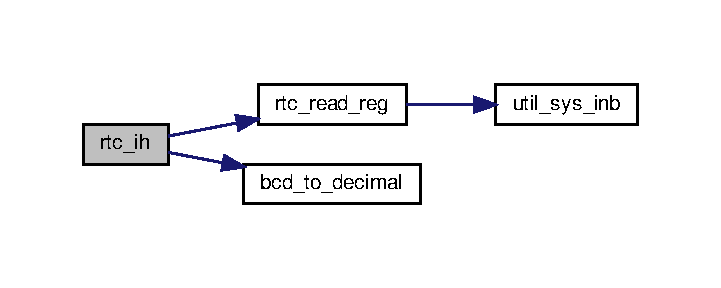
\includegraphics[width=346pt]{group__rtc_ga55d98e39c0c2bf246ef774491c31b593_cgraph}
\end{center}
\end{figure}
\mbox{\Hypertarget{group__rtc_gaacd5a961df48ee02b0d95588cbe00be5}\label{group__rtc_gaacd5a961df48ee02b0d95588cbe00be5}} 
\index{rtc@{rtc}!rtc\+\_\+ih\+\_\+disable@{rtc\+\_\+ih\+\_\+disable}}
\index{rtc\+\_\+ih\+\_\+disable@{rtc\+\_\+ih\+\_\+disable}!rtc@{rtc}}
\subsubsection{\texorpdfstring{rtc\+\_\+ih\+\_\+disable()}{rtc\_ih\_disable()}}
{\footnotesize\ttfamily int rtc\+\_\+ih\+\_\+disable (\begin{DoxyParamCaption}{ }\end{DoxyParamCaption})}



Disables R\+TC interrupts. 

\begin{DoxyReturn}{Returns}
0 if successful, otherwise it was not successful 
\end{DoxyReturn}
\mbox{\Hypertarget{group__rtc_ga272e00608ea1e5f0e931ae7a566c2af4}\label{group__rtc_ga272e00608ea1e5f0e931ae7a566c2af4}} 
\index{rtc@{rtc}!rtc\+\_\+ih\+\_\+enable@{rtc\+\_\+ih\+\_\+enable}}
\index{rtc\+\_\+ih\+\_\+enable@{rtc\+\_\+ih\+\_\+enable}!rtc@{rtc}}
\subsubsection{\texorpdfstring{rtc\+\_\+ih\+\_\+enable()}{rtc\_ih\_enable()}}
{\footnotesize\ttfamily int rtc\+\_\+ih\+\_\+enable (\begin{DoxyParamCaption}{ }\end{DoxyParamCaption})}



Enables R\+TC interrupts. 

\begin{DoxyReturn}{Returns}
0 if successful, otherwise it was not successful 
\end{DoxyReturn}
\mbox{\Hypertarget{group__rtc_gaa9a633f60d6ee3b237a80b408647908c}\label{group__rtc_gaa9a633f60d6ee3b237a80b408647908c}} 
\index{rtc@{rtc}!rtc\+\_\+ih\+\_\+subscribe@{rtc\+\_\+ih\+\_\+subscribe}}
\index{rtc\+\_\+ih\+\_\+subscribe@{rtc\+\_\+ih\+\_\+subscribe}!rtc@{rtc}}
\subsubsection{\texorpdfstring{rtc\+\_\+ih\+\_\+subscribe()}{rtc\_ih\_subscribe()}}
{\footnotesize\ttfamily int rtc\+\_\+ih\+\_\+subscribe (\begin{DoxyParamCaption}{ }\end{DoxyParamCaption})}



Subscribes to R\+TC interrupts. 

\begin{DoxyReturn}{Returns}
0 if successful, otherwise it was not successful 
\end{DoxyReturn}
\mbox{\Hypertarget{group__rtc_ga9c629cc80f25b7d9d4e19fb6f6de8ea4}\label{group__rtc_ga9c629cc80f25b7d9d4e19fb6f6de8ea4}} 
\index{rtc@{rtc}!rtc\+\_\+ih\+\_\+unsubscribe@{rtc\+\_\+ih\+\_\+unsubscribe}}
\index{rtc\+\_\+ih\+\_\+unsubscribe@{rtc\+\_\+ih\+\_\+unsubscribe}!rtc@{rtc}}
\subsubsection{\texorpdfstring{rtc\+\_\+ih\+\_\+unsubscribe()}{rtc\_ih\_unsubscribe()}}
{\footnotesize\ttfamily int rtc\+\_\+ih\+\_\+unsubscribe (\begin{DoxyParamCaption}{ }\end{DoxyParamCaption})}



Unsubscribes to R\+TC interrupts. 

\begin{DoxyReturn}{Returns}
0 if successful, otherwise it was not successful 
\end{DoxyReturn}
\mbox{\Hypertarget{group__rtc_ga967406c372c2ba0b6b18c4784d5b1ce2}\label{group__rtc_ga967406c372c2ba0b6b18c4784d5b1ce2}} 
\index{rtc@{rtc}!rtc\+\_\+read\+\_\+reg@{rtc\+\_\+read\+\_\+reg}}
\index{rtc\+\_\+read\+\_\+reg@{rtc\+\_\+read\+\_\+reg}!rtc@{rtc}}
\subsubsection{\texorpdfstring{rtc\+\_\+read\+\_\+reg()}{rtc\_read\_reg()}}
{\footnotesize\ttfamily uint8\+\_\+t rtc\+\_\+read\+\_\+reg (\begin{DoxyParamCaption}\item[{uint8\+\_\+t}]{reg }\end{DoxyParamCaption})}



Reads the R\+TC register at position reg. 


\begin{DoxyParams}{Parameters}
{\em reg} & The register to be read \\
\hline
\end{DoxyParams}
\begin{DoxyReturn}{Returns}
The byte of the register at position reg 
\end{DoxyReturn}
Here is the call graph for this function\+:\nopagebreak
\begin{figure}[H]
\begin{center}
\leavevmode
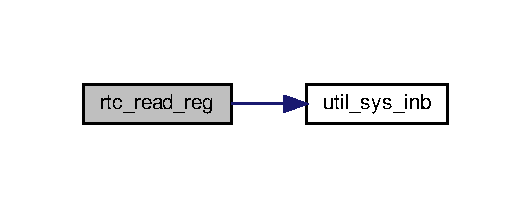
\includegraphics[width=255pt]{group__rtc_ga967406c372c2ba0b6b18c4784d5b1ce2_cgraph}
\end{center}
\end{figure}
\mbox{\Hypertarget{group__rtc_ga9d32737436e666dcd33816dd240321a8}\label{group__rtc_ga9d32737436e666dcd33816dd240321a8}} 
\index{rtc@{rtc}!rtc\+\_\+write\+\_\+reg@{rtc\+\_\+write\+\_\+reg}}
\index{rtc\+\_\+write\+\_\+reg@{rtc\+\_\+write\+\_\+reg}!rtc@{rtc}}
\subsubsection{\texorpdfstring{rtc\+\_\+write\+\_\+reg()}{rtc\_write\_reg()}}
{\footnotesize\ttfamily void rtc\+\_\+write\+\_\+reg (\begin{DoxyParamCaption}\item[{uint8\+\_\+t}]{reg,  }\item[{uint8\+\_\+t}]{data }\end{DoxyParamCaption})}



Writes the R\+TC register at position reg. 


\begin{DoxyParams}{Parameters}
{\em reg} & The register to be written \\
\hline
{\em data} & The byte that is going to be written in the register \\
\hline
\end{DoxyParams}

\hypertarget{group__timer}{}\section{timer}
\label{group__timer}\index{timer@{timer}}


Timer interrupt-\/related functions.  


\subsection*{Macros}
\begin{DoxyCompactItemize}
\item 
\#define \hyperlink{group__timer_ga6afdd2bea8e7518daaa2641def6638a5}{T\+I\+M\+E\+R\+\_\+\+I\+N\+T\+E\+R\+R\+U\+P\+T\+\_\+\+F\+R\+EQ}~60
\item 
\#define \hyperlink{group__timer_ga7095fb363d08f6646611f9a47806647b}{T\+I\+M\+E\+R\+\_\+\+I\+RQ}~0
\item 
\#define \hyperlink{group__timer_gacaa139b4a451d80a4cb00da3451edd5b}{T\+I\+M\+E\+R\+\_\+\+H\+O\+O\+K\+\_\+\+ID}~0
\item 
\#define \hyperlink{group__timer_gae41604e470c014060c92349437078e03}{T\+I\+M\+E\+R\+\_\+\+M\+A\+SK}~B\+IT(\hyperlink{group__timer_gacaa139b4a451d80a4cb00da3451edd5b}{T\+I\+M\+E\+R\+\_\+\+H\+O\+O\+K\+\_\+\+ID})
\end{DoxyCompactItemize}
\subsection*{Functions}
\begin{DoxyCompactItemize}
\item 
int \hyperlink{group__timer_gacbda5965336eef31790e7a8b983332ff}{timer\+\_\+get\+\_\+counter} ()
\item 
int \hyperlink{group__timer_gae44be0cfa0b6e717152afc708577cf5d}{timer\+\_\+ih\+\_\+subscribe} ()
\begin{DoxyCompactList}\small\item\em Subscribes to timer interrupts. \end{DoxyCompactList}\item 
int \hyperlink{group__timer_ga5e9cfb5b4e41a1e647e0ee7d0ed6709a}{timer\+\_\+ih\+\_\+unsubscribe} ()
\begin{DoxyCompactList}\small\item\em Unsubscribes to timer interrupts. \end{DoxyCompactList}\item 
int \hyperlink{group__timer_ga4baf1b5c30d394576f8044178524e2c4}{timer\+\_\+ih\+\_\+enable} ()
\begin{DoxyCompactList}\small\item\em Enables timer interrupts. \end{DoxyCompactList}\item 
int \hyperlink{group__timer_ga4a90bd229401205fbf0222cc3228c22c}{timer\+\_\+ih\+\_\+disable} ()
\begin{DoxyCompactList}\small\item\em Disables timer interrupts. \end{DoxyCompactList}\end{DoxyCompactItemize}


\subsection{Detailed Description}
Timer interrupt-\/related functions. 



\subsection{Macro Definition Documentation}
\mbox{\Hypertarget{group__timer_gacaa139b4a451d80a4cb00da3451edd5b}\label{group__timer_gacaa139b4a451d80a4cb00da3451edd5b}} 
\index{timer@{timer}!T\+I\+M\+E\+R\+\_\+\+H\+O\+O\+K\+\_\+\+ID@{T\+I\+M\+E\+R\+\_\+\+H\+O\+O\+K\+\_\+\+ID}}
\index{T\+I\+M\+E\+R\+\_\+\+H\+O\+O\+K\+\_\+\+ID@{T\+I\+M\+E\+R\+\_\+\+H\+O\+O\+K\+\_\+\+ID}!timer@{timer}}
\subsubsection{\texorpdfstring{T\+I\+M\+E\+R\+\_\+\+H\+O\+O\+K\+\_\+\+ID}{TIMER\_HOOK\_ID}}
{\footnotesize\ttfamily \#define T\+I\+M\+E\+R\+\_\+\+H\+O\+O\+K\+\_\+\+ID~0}

\mbox{\Hypertarget{group__timer_ga6afdd2bea8e7518daaa2641def6638a5}\label{group__timer_ga6afdd2bea8e7518daaa2641def6638a5}} 
\index{timer@{timer}!T\+I\+M\+E\+R\+\_\+\+I\+N\+T\+E\+R\+R\+U\+P\+T\+\_\+\+F\+R\+EQ@{T\+I\+M\+E\+R\+\_\+\+I\+N\+T\+E\+R\+R\+U\+P\+T\+\_\+\+F\+R\+EQ}}
\index{T\+I\+M\+E\+R\+\_\+\+I\+N\+T\+E\+R\+R\+U\+P\+T\+\_\+\+F\+R\+EQ@{T\+I\+M\+E\+R\+\_\+\+I\+N\+T\+E\+R\+R\+U\+P\+T\+\_\+\+F\+R\+EQ}!timer@{timer}}
\subsubsection{\texorpdfstring{T\+I\+M\+E\+R\+\_\+\+I\+N\+T\+E\+R\+R\+U\+P\+T\+\_\+\+F\+R\+EQ}{TIMER\_INTERRUPT\_FREQ}}
{\footnotesize\ttfamily \#define T\+I\+M\+E\+R\+\_\+\+I\+N\+T\+E\+R\+R\+U\+P\+T\+\_\+\+F\+R\+EQ~60}

\mbox{\Hypertarget{group__timer_ga7095fb363d08f6646611f9a47806647b}\label{group__timer_ga7095fb363d08f6646611f9a47806647b}} 
\index{timer@{timer}!T\+I\+M\+E\+R\+\_\+\+I\+RQ@{T\+I\+M\+E\+R\+\_\+\+I\+RQ}}
\index{T\+I\+M\+E\+R\+\_\+\+I\+RQ@{T\+I\+M\+E\+R\+\_\+\+I\+RQ}!timer@{timer}}
\subsubsection{\texorpdfstring{T\+I\+M\+E\+R\+\_\+\+I\+RQ}{TIMER\_IRQ}}
{\footnotesize\ttfamily \#define T\+I\+M\+E\+R\+\_\+\+I\+RQ~0}

\mbox{\Hypertarget{group__timer_gae41604e470c014060c92349437078e03}\label{group__timer_gae41604e470c014060c92349437078e03}} 
\index{timer@{timer}!T\+I\+M\+E\+R\+\_\+\+M\+A\+SK@{T\+I\+M\+E\+R\+\_\+\+M\+A\+SK}}
\index{T\+I\+M\+E\+R\+\_\+\+M\+A\+SK@{T\+I\+M\+E\+R\+\_\+\+M\+A\+SK}!timer@{timer}}
\subsubsection{\texorpdfstring{T\+I\+M\+E\+R\+\_\+\+M\+A\+SK}{TIMER\_MASK}}
{\footnotesize\ttfamily \#define T\+I\+M\+E\+R\+\_\+\+M\+A\+SK~B\+IT(\hyperlink{group__timer_gacaa139b4a451d80a4cb00da3451edd5b}{T\+I\+M\+E\+R\+\_\+\+H\+O\+O\+K\+\_\+\+ID})}



\subsection{Function Documentation}
\mbox{\Hypertarget{group__timer_gacbda5965336eef31790e7a8b983332ff}\label{group__timer_gacbda5965336eef31790e7a8b983332ff}} 
\index{timer@{timer}!timer\+\_\+get\+\_\+counter@{timer\+\_\+get\+\_\+counter}}
\index{timer\+\_\+get\+\_\+counter@{timer\+\_\+get\+\_\+counter}!timer@{timer}}
\subsubsection{\texorpdfstring{timer\+\_\+get\+\_\+counter()}{timer\_get\_counter()}}
{\footnotesize\ttfamily int timer\+\_\+get\+\_\+counter (\begin{DoxyParamCaption}{ }\end{DoxyParamCaption})}

\begin{DoxyReturn}{Returns}
The number of interrupts the timer has triggered 
\end{DoxyReturn}
\mbox{\Hypertarget{group__timer_ga4a90bd229401205fbf0222cc3228c22c}\label{group__timer_ga4a90bd229401205fbf0222cc3228c22c}} 
\index{timer@{timer}!timer\+\_\+ih\+\_\+disable@{timer\+\_\+ih\+\_\+disable}}
\index{timer\+\_\+ih\+\_\+disable@{timer\+\_\+ih\+\_\+disable}!timer@{timer}}
\subsubsection{\texorpdfstring{timer\+\_\+ih\+\_\+disable()}{timer\_ih\_disable()}}
{\footnotesize\ttfamily int timer\+\_\+ih\+\_\+disable (\begin{DoxyParamCaption}{ }\end{DoxyParamCaption})}



Disables timer interrupts. 

\begin{DoxyReturn}{Returns}
0 if successful, otherwise it was not successful 
\end{DoxyReturn}
\mbox{\Hypertarget{group__timer_ga4baf1b5c30d394576f8044178524e2c4}\label{group__timer_ga4baf1b5c30d394576f8044178524e2c4}} 
\index{timer@{timer}!timer\+\_\+ih\+\_\+enable@{timer\+\_\+ih\+\_\+enable}}
\index{timer\+\_\+ih\+\_\+enable@{timer\+\_\+ih\+\_\+enable}!timer@{timer}}
\subsubsection{\texorpdfstring{timer\+\_\+ih\+\_\+enable()}{timer\_ih\_enable()}}
{\footnotesize\ttfamily int timer\+\_\+ih\+\_\+enable (\begin{DoxyParamCaption}{ }\end{DoxyParamCaption})}



Enables timer interrupts. 

\begin{DoxyReturn}{Returns}
0 if successful, otherwise it was not successful 
\end{DoxyReturn}
\mbox{\Hypertarget{group__timer_gae44be0cfa0b6e717152afc708577cf5d}\label{group__timer_gae44be0cfa0b6e717152afc708577cf5d}} 
\index{timer@{timer}!timer\+\_\+ih\+\_\+subscribe@{timer\+\_\+ih\+\_\+subscribe}}
\index{timer\+\_\+ih\+\_\+subscribe@{timer\+\_\+ih\+\_\+subscribe}!timer@{timer}}
\subsubsection{\texorpdfstring{timer\+\_\+ih\+\_\+subscribe()}{timer\_ih\_subscribe()}}
{\footnotesize\ttfamily int timer\+\_\+ih\+\_\+subscribe (\begin{DoxyParamCaption}{ }\end{DoxyParamCaption})}



Subscribes to timer interrupts. 

\begin{DoxyReturn}{Returns}
0 if successful, otherwise it was not successful 
\end{DoxyReturn}
\mbox{\Hypertarget{group__timer_ga5e9cfb5b4e41a1e647e0ee7d0ed6709a}\label{group__timer_ga5e9cfb5b4e41a1e647e0ee7d0ed6709a}} 
\index{timer@{timer}!timer\+\_\+ih\+\_\+unsubscribe@{timer\+\_\+ih\+\_\+unsubscribe}}
\index{timer\+\_\+ih\+\_\+unsubscribe@{timer\+\_\+ih\+\_\+unsubscribe}!timer@{timer}}
\subsubsection{\texorpdfstring{timer\+\_\+ih\+\_\+unsubscribe()}{timer\_ih\_unsubscribe()}}
{\footnotesize\ttfamily int timer\+\_\+ih\+\_\+unsubscribe (\begin{DoxyParamCaption}{ }\end{DoxyParamCaption})}



Unsubscribes to timer interrupts. 

\begin{DoxyReturn}{Returns}
0 if successful, otherwise it was not successful 
\end{DoxyReturn}

\hypertarget{group__triangle}{}\section{triangle}
\label{group__triangle}\index{triangle@{triangle}}


Triangle drawing and collision-\/checking functions.  


\subsection*{Functions}
\begin{DoxyCompactItemize}
\item 
void \hyperlink{group__triangle_ga7debe2af7dc5ecd4b384f7c1b254c38c}{triangle\+\_\+draw} (uint8\+\_\+t $\ast$base\+\_\+ptr, int16\+\_\+t x1, int16\+\_\+t y1, int16\+\_\+t x2, int16\+\_\+t y2, int16\+\_\+t x3, int16\+\_\+t y3, uint32\+\_\+t color)
\begin{DoxyCompactList}\small\item\em Draws a triangle on the given buffer with the given vertices and color. \end{DoxyCompactList}\item 
bool \hyperlink{group__triangle_gaa849ba110cf7f4a6199c4a728b0084f1}{check\+\_\+pixel} (float x\+\_\+pixel, float y\+\_\+pixel, float x1, float y1, float x2, float y2, float x3, float y3)
\begin{DoxyCompactList}\small\item\em Checks whether or not a given point is inside a triangle. \end{DoxyCompactList}\end{DoxyCompactItemize}


\subsection{Detailed Description}
Triangle drawing and collision-\/checking functions. 



\subsection{Function Documentation}
\mbox{\Hypertarget{group__triangle_gaa849ba110cf7f4a6199c4a728b0084f1}\label{group__triangle_gaa849ba110cf7f4a6199c4a728b0084f1}} 
\index{triangle@{triangle}!check\+\_\+pixel@{check\+\_\+pixel}}
\index{check\+\_\+pixel@{check\+\_\+pixel}!triangle@{triangle}}
\subsubsection{\texorpdfstring{check\+\_\+pixel()}{check\_pixel()}}
{\footnotesize\ttfamily bool check\+\_\+pixel (\begin{DoxyParamCaption}\item[{float}]{x\+\_\+pixel,  }\item[{float}]{y\+\_\+pixel,  }\item[{float}]{x1,  }\item[{float}]{y1,  }\item[{float}]{x2,  }\item[{float}]{y2,  }\item[{float}]{x3,  }\item[{float}]{y3 }\end{DoxyParamCaption})}



Checks whether or not a given point is inside a triangle. 


\begin{DoxyParams}{Parameters}
{\em x\+\_\+pixel} & The x coordinate of the point to be checked \\
\hline
{\em y\+\_\+pixel} & The y coordinate of the point to be checked \\
\hline
{\em x1} & The x coordinate of the first vertex of the triangle \\
\hline
{\em y1} & The y coordinate of the first vertex of the triangle \\
\hline
{\em x2} & The x coordinate of the second vertex of the triangle \\
\hline
{\em y2} & The y coordinate of the second vertex of the triangle \\
\hline
{\em x3} & The x coordinate of the third vertex of the triangle \\
\hline
{\em y3} & The y coordinate of the third vertex of the triangle\\
\hline
\end{DoxyParams}
\begin{DoxyReturn}{Returns}
true if the pixel is inside of the triangle, otherwise false 
\end{DoxyReturn}
\mbox{\Hypertarget{group__triangle_ga7debe2af7dc5ecd4b384f7c1b254c38c}\label{group__triangle_ga7debe2af7dc5ecd4b384f7c1b254c38c}} 
\index{triangle@{triangle}!triangle\+\_\+draw@{triangle\+\_\+draw}}
\index{triangle\+\_\+draw@{triangle\+\_\+draw}!triangle@{triangle}}
\subsubsection{\texorpdfstring{triangle\+\_\+draw()}{triangle\_draw()}}
{\footnotesize\ttfamily void triangle\+\_\+draw (\begin{DoxyParamCaption}\item[{uint8\+\_\+t $\ast$}]{base\+\_\+ptr,  }\item[{int16\+\_\+t}]{x1,  }\item[{int16\+\_\+t}]{y1,  }\item[{int16\+\_\+t}]{x2,  }\item[{int16\+\_\+t}]{y2,  }\item[{int16\+\_\+t}]{x3,  }\item[{int16\+\_\+t}]{y3,  }\item[{uint32\+\_\+t}]{color }\end{DoxyParamCaption})}



Draws a triangle on the given buffer with the given vertices and color. 


\begin{DoxyParams}{Parameters}
{\em base\+\_\+ptr} & A pointer to a buffer (must be equal in size to the frame buffer) \\
\hline
{\em x1} & The x coordinate of the first vertex \\
\hline
{\em y1} & The y coordinate of the first vertex \\
\hline
{\em x2} & The x coordinate of the second vertex \\
\hline
{\em y2} & The y coordinate of the second vertex \\
\hline
{\em x3} & The x coordinate of the third vertex \\
\hline
{\em y3} & The y coordinate of the third vertex \\
\hline
{\em color} & The color of the triangle \\
\hline
\end{DoxyParams}
Here is the call graph for this function\+:\nopagebreak
\begin{figure}[H]
\begin{center}
\leavevmode
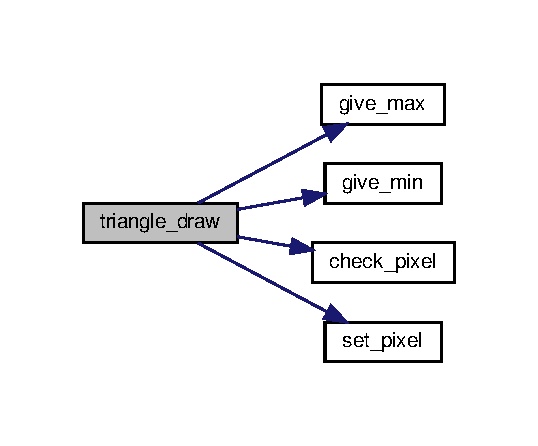
\includegraphics[width=258pt]{group__triangle_ga7debe2af7dc5ecd4b384f7c1b254c38c_cgraph}
\end{center}
\end{figure}

\hypertarget{group__utils}{}\section{utils}
\label{group__utils}\index{utils@{utils}}


Utility functions.  


\subsection*{Functions}
\begin{DoxyCompactItemize}
\item 
int \hyperlink{group__utils_ga2b56f50ba159e9d5115ed1a75eff15d9}{util\+\_\+sys\+\_\+inb} (int port, uint8\+\_\+t $\ast$value)
\begin{DoxyCompactList}\small\item\em Reads a byte from memory. \end{DoxyCompactList}\item 
uint8\+\_\+t \hyperlink{group__utils_ga304fc85c5c7fb06010deb07c6dd16b81}{bcd\+\_\+to\+\_\+decimal} (uint8\+\_\+t hex)
\begin{DoxyCompactList}\small\item\em Converts a value from bcd format to decimal format. \end{DoxyCompactList}\item 
uint8\+\_\+t \hyperlink{group__utils_ga8c10bb1f9a5bb82b67c6980182193c54}{decimal\+\_\+to\+\_\+bcd} (uint8\+\_\+t decimal)
\begin{DoxyCompactList}\small\item\em Converts a value from decimal format to bcd format. \end{DoxyCompactList}\end{DoxyCompactItemize}


\subsection{Detailed Description}
Utility functions. 



\subsection{Function Documentation}
\mbox{\Hypertarget{group__utils_ga304fc85c5c7fb06010deb07c6dd16b81}\label{group__utils_ga304fc85c5c7fb06010deb07c6dd16b81}} 
\index{utils@{utils}!bcd\+\_\+to\+\_\+decimal@{bcd\+\_\+to\+\_\+decimal}}
\index{bcd\+\_\+to\+\_\+decimal@{bcd\+\_\+to\+\_\+decimal}!utils@{utils}}
\subsubsection{\texorpdfstring{bcd\+\_\+to\+\_\+decimal()}{bcd\_to\_decimal()}}
{\footnotesize\ttfamily uint8\+\_\+t bcd\+\_\+to\+\_\+decimal (\begin{DoxyParamCaption}\item[{uint8\+\_\+t}]{hex }\end{DoxyParamCaption})}



Converts a value from bcd format to decimal format. 


\begin{DoxyParams}{Parameters}
{\em hex} & The value in bcd format\\
\hline
\end{DoxyParams}
\begin{DoxyReturn}{Returns}
The value in decimal format 
\end{DoxyReturn}
\mbox{\Hypertarget{group__utils_ga8c10bb1f9a5bb82b67c6980182193c54}\label{group__utils_ga8c10bb1f9a5bb82b67c6980182193c54}} 
\index{utils@{utils}!decimal\+\_\+to\+\_\+bcd@{decimal\+\_\+to\+\_\+bcd}}
\index{decimal\+\_\+to\+\_\+bcd@{decimal\+\_\+to\+\_\+bcd}!utils@{utils}}
\subsubsection{\texorpdfstring{decimal\+\_\+to\+\_\+bcd()}{decimal\_to\_bcd()}}
{\footnotesize\ttfamily uint8\+\_\+t decimal\+\_\+to\+\_\+bcd (\begin{DoxyParamCaption}\item[{uint8\+\_\+t}]{decimal }\end{DoxyParamCaption})}



Converts a value from decimal format to bcd format. 


\begin{DoxyParams}{Parameters}
{\em decimal} & The value in decimal format\\
\hline
\end{DoxyParams}
\begin{DoxyReturn}{Returns}
The value in bcd format 
\end{DoxyReturn}
\mbox{\Hypertarget{group__utils_ga2b56f50ba159e9d5115ed1a75eff15d9}\label{group__utils_ga2b56f50ba159e9d5115ed1a75eff15d9}} 
\index{utils@{utils}!util\+\_\+sys\+\_\+inb@{util\+\_\+sys\+\_\+inb}}
\index{util\+\_\+sys\+\_\+inb@{util\+\_\+sys\+\_\+inb}!utils@{utils}}
\subsubsection{\texorpdfstring{util\+\_\+sys\+\_\+inb()}{util\_sys\_inb()}}
{\footnotesize\ttfamily int util\+\_\+sys\+\_\+inb (\begin{DoxyParamCaption}\item[{int}]{port,  }\item[{uint8\+\_\+t $\ast$}]{value }\end{DoxyParamCaption})}



Reads a byte from memory. 


\begin{DoxyParams}{Parameters}
{\em port} & The memory address (normally in hexadecimal) \\
\hline
{\em value} & A pointer to a byte, which will be rewritten with the value in memory\\
\hline
\end{DoxyParams}
\begin{DoxyReturn}{Returns}
0 if successful, otherwise it was not successful 
\end{DoxyReturn}

\hypertarget{group__vector2}{}\section{vector2}
\label{group__vector2}\index{vector2@{vector2}}


Functions for 2-\/dimensional vector manipulations.  


\subsection*{Data Structures}
\begin{DoxyCompactItemize}
\item 
struct \hyperlink{structvector2}{vector2}
\begin{DoxyCompactList}\small\item\em Struct that represents a vector in 2d space. \end{DoxyCompactList}\end{DoxyCompactItemize}
\subsection*{Typedefs}
\begin{DoxyCompactItemize}
\item 
typedef struct \hyperlink{structvector2}{vector2} \hyperlink{group__vector2_ga79bfbffebc693e35657aa7eec9499688}{vector2}
\begin{DoxyCompactList}\small\item\em Struct that represents a vector in 2d space. \end{DoxyCompactList}\end{DoxyCompactItemize}
\subsection*{Functions}
\begin{DoxyCompactItemize}
\item 
\hyperlink{structvector2}{vector2} \hyperlink{group__vector2_ga8a53b9698cf1172ab388531dcd3d8399}{vector2\+\_\+add} (\hyperlink{structvector2}{vector2} v1, \hyperlink{structvector2}{vector2} v2)
\item 
\hyperlink{structvector2}{vector2} \hyperlink{group__vector2_ga7a403a2bce25c9ee0fd5e6fc30a8f9ea}{vector2\+\_\+subtract} (\hyperlink{structvector2}{vector2} v1, \hyperlink{structvector2}{vector2} v2)
\item 
\hyperlink{structvector2}{vector2} \hyperlink{group__vector2_gab71f45ca9825acdbf70c639cf4a5d09c}{vector2\+\_\+scalar\+\_\+product} (\hyperlink{structvector2}{vector2} v, float k)
\item 
float \hyperlink{group__vector2_ga03173bb05b63e8723fc6e54cf55dff71}{vector2\+\_\+norm} (\hyperlink{structvector2}{vector2} v)
\item 
\hyperlink{structvector2}{vector2} \hyperlink{group__vector2_gaa3e831b3dbed8e51233f48de98c3266e}{vector2\+\_\+normalized} (\hyperlink{structvector2}{vector2} v)
\end{DoxyCompactItemize}


\subsection{Detailed Description}
Functions for 2-\/dimensional vector manipulations. 



\subsection{Typedef Documentation}
\mbox{\Hypertarget{group__vector2_ga79bfbffebc693e35657aa7eec9499688}\label{group__vector2_ga79bfbffebc693e35657aa7eec9499688}} 
\index{vector2@{vector2}!vector2@{vector2}}
\index{vector2@{vector2}!vector2@{vector2}}
\subsubsection{\texorpdfstring{vector2}{vector2}}
{\footnotesize\ttfamily typedef struct \hyperlink{structvector2}{vector2}  \hyperlink{structvector2}{vector2}}



Struct that represents a vector in 2d space. 



\subsection{Function Documentation}
\mbox{\Hypertarget{group__vector2_ga8a53b9698cf1172ab388531dcd3d8399}\label{group__vector2_ga8a53b9698cf1172ab388531dcd3d8399}} 
\index{vector2@{vector2}!vector2\+\_\+add@{vector2\+\_\+add}}
\index{vector2\+\_\+add@{vector2\+\_\+add}!vector2@{vector2}}
\subsubsection{\texorpdfstring{vector2\+\_\+add()}{vector2\_add()}}
{\footnotesize\ttfamily \hyperlink{structvector2}{vector2} vector2\+\_\+add (\begin{DoxyParamCaption}\item[{\hyperlink{structvector2}{vector2}}]{v1,  }\item[{\hyperlink{structvector2}{vector2}}]{v2 }\end{DoxyParamCaption})}

\begin{DoxyReturn}{Returns}
The sum of v1 and v2 
\end{DoxyReturn}
\mbox{\Hypertarget{group__vector2_ga03173bb05b63e8723fc6e54cf55dff71}\label{group__vector2_ga03173bb05b63e8723fc6e54cf55dff71}} 
\index{vector2@{vector2}!vector2\+\_\+norm@{vector2\+\_\+norm}}
\index{vector2\+\_\+norm@{vector2\+\_\+norm}!vector2@{vector2}}
\subsubsection{\texorpdfstring{vector2\+\_\+norm()}{vector2\_norm()}}
{\footnotesize\ttfamily float vector2\+\_\+norm (\begin{DoxyParamCaption}\item[{\hyperlink{structvector2}{vector2}}]{v }\end{DoxyParamCaption})}

\begin{DoxyReturn}{Returns}
The lenght of \hyperlink{structvector2}{vector2} v 
\end{DoxyReturn}
\mbox{\Hypertarget{group__vector2_gaa3e831b3dbed8e51233f48de98c3266e}\label{group__vector2_gaa3e831b3dbed8e51233f48de98c3266e}} 
\index{vector2@{vector2}!vector2\+\_\+normalized@{vector2\+\_\+normalized}}
\index{vector2\+\_\+normalized@{vector2\+\_\+normalized}!vector2@{vector2}}
\subsubsection{\texorpdfstring{vector2\+\_\+normalized()}{vector2\_normalized()}}
{\footnotesize\ttfamily \hyperlink{structvector2}{vector2} vector2\+\_\+normalized (\begin{DoxyParamCaption}\item[{\hyperlink{structvector2}{vector2}}]{v }\end{DoxyParamCaption})}

\begin{DoxyReturn}{Returns}
The normalized version of \hyperlink{structvector2}{vector2} v 
\end{DoxyReturn}
Here is the call graph for this function\+:\nopagebreak
\begin{figure}[H]
\begin{center}
\leavevmode
\includegraphics[width=293pt]{group__vector2_gaa3e831b3dbed8e51233f48de98c3266e_cgraph}
\end{center}
\end{figure}
\mbox{\Hypertarget{group__vector2_gab71f45ca9825acdbf70c639cf4a5d09c}\label{group__vector2_gab71f45ca9825acdbf70c639cf4a5d09c}} 
\index{vector2@{vector2}!vector2\+\_\+scalar\+\_\+product@{vector2\+\_\+scalar\+\_\+product}}
\index{vector2\+\_\+scalar\+\_\+product@{vector2\+\_\+scalar\+\_\+product}!vector2@{vector2}}
\subsubsection{\texorpdfstring{vector2\+\_\+scalar\+\_\+product()}{vector2\_scalar\_product()}}
{\footnotesize\ttfamily \hyperlink{structvector2}{vector2} vector2\+\_\+scalar\+\_\+product (\begin{DoxyParamCaption}\item[{\hyperlink{structvector2}{vector2}}]{v,  }\item[{float}]{k }\end{DoxyParamCaption})}

\begin{DoxyReturn}{Returns}
A \hyperlink{structvector2}{vector2} in which every element of v is multiplied by k 
\end{DoxyReturn}
\mbox{\Hypertarget{group__vector2_ga7a403a2bce25c9ee0fd5e6fc30a8f9ea}\label{group__vector2_ga7a403a2bce25c9ee0fd5e6fc30a8f9ea}} 
\index{vector2@{vector2}!vector2\+\_\+subtract@{vector2\+\_\+subtract}}
\index{vector2\+\_\+subtract@{vector2\+\_\+subtract}!vector2@{vector2}}
\subsubsection{\texorpdfstring{vector2\+\_\+subtract()}{vector2\_subtract()}}
{\footnotesize\ttfamily \hyperlink{structvector2}{vector2} vector2\+\_\+subtract (\begin{DoxyParamCaption}\item[{\hyperlink{structvector2}{vector2}}]{v1,  }\item[{\hyperlink{structvector2}{vector2}}]{v2 }\end{DoxyParamCaption})}

\begin{DoxyReturn}{Returns}
v1 subtracted by v2 
\end{DoxyReturn}

\hypertarget{group__video__card}{}\section{video\+\_\+card}
\label{group__video__card}\index{video\+\_\+card@{video\+\_\+card}}


Functions related to graphic mode initialization and frame buffer modification.  


\subsection*{Functions}
\begin{DoxyCompactItemize}
\item 
uint16\+\_\+t \hyperlink{group__video__card_gad5999dee7ae30ea14b13e2e2e5a92c88}{get\+\_\+vres} ()
\item 
uint16\+\_\+t \hyperlink{group__video__card_ga8becb86f48f701c43e1c411f57f60c4d}{get\+\_\+hres} ()
\item 
uint16\+\_\+t \hyperlink{group__video__card_ga9f914dcc3574459a6f0f5fa903ad40e7}{get\+\_\+bytes\+\_\+per\+\_\+pixel} ()
\item 
uint16\+\_\+t \hyperlink{group__video__card_ga3ff6bb40b256e97af89a53bd459b59f5}{get\+\_\+buffer\+\_\+size} ()
\item 
uint8\+\_\+t $\ast$ \hyperlink{group__video__card_ga461fb4a3b5536b3de26e342444394ddd}{get\+\_\+buffer\+\_\+base\+\_\+ptr} ()
\item 
void \hyperlink{group__video__card_ga5f6f4feebf127c7d02258175e5df35ff}{set\+\_\+pixel} (uint8\+\_\+t $\ast$base\+\_\+ptr, uint16\+\_\+t x, uint16\+\_\+t y, uint32\+\_\+t color)
\begin{DoxyCompactList}\small\item\em Sets the pixel of the given buffer at the given coordinates to the given color. \end{DoxyCompactList}\item 
void \hyperlink{group__video__card_ga88795d0238c894e7d54c134b69305976}{set\+\_\+rectangle} (uint8\+\_\+t $\ast$base\+\_\+ptr, uint16\+\_\+t x, uint16\+\_\+t y, uint16\+\_\+t len\+\_\+x, uint16\+\_\+t len\+\_\+y, uint32\+\_\+t color)
\begin{DoxyCompactList}\small\item\em Draws a rectangle on the given buffer at the given coordinates with the given lenght and height to the given color. \end{DoxyCompactList}\item 
void \hyperlink{group__video__card_gacd25f5efb8e27da60488e6b317be5e12}{set\+\_\+xpm\+\_\+image} (uint8\+\_\+t $\ast$base\+\_\+ptr, uint16\+\_\+t x, uint16\+\_\+t y, xpm\+\_\+image\+\_\+t img)
\begin{DoxyCompactList}\small\item\em Draws the given xpm image on the given buffer at the given coordinates. \end{DoxyCompactList}\item 
void \hyperlink{group__video__card_ga0d199b5702695c4d7b78ef83759c32d5}{clean\+\_\+screen} ()
\begin{DoxyCompactList}\small\item\em Sets all the bytes of the frame buffer to 0, meaning that the screen turns black. \end{DoxyCompactList}\end{DoxyCompactItemize}


\subsection{Detailed Description}
Functions related to graphic mode initialization and frame buffer modification. 

All the functions provided have buffer boundary checks, which means that they are (as far as I\textquotesingle{}m concerned) safe to use given bogus coordinates 

\subsection{Function Documentation}
\mbox{\Hypertarget{group__video__card_ga0d199b5702695c4d7b78ef83759c32d5}\label{group__video__card_ga0d199b5702695c4d7b78ef83759c32d5}} 
\index{video\+\_\+card@{video\+\_\+card}!clean\+\_\+screen@{clean\+\_\+screen}}
\index{clean\+\_\+screen@{clean\+\_\+screen}!video\+\_\+card@{video\+\_\+card}}
\subsubsection{\texorpdfstring{clean\+\_\+screen()}{clean\_screen()}}
{\footnotesize\ttfamily void clean\+\_\+screen (\begin{DoxyParamCaption}{ }\end{DoxyParamCaption})}



Sets all the bytes of the frame buffer to 0, meaning that the screen turns black. 

\mbox{\Hypertarget{group__video__card_ga461fb4a3b5536b3de26e342444394ddd}\label{group__video__card_ga461fb4a3b5536b3de26e342444394ddd}} 
\index{video\+\_\+card@{video\+\_\+card}!get\+\_\+buffer\+\_\+base\+\_\+ptr@{get\+\_\+buffer\+\_\+base\+\_\+ptr}}
\index{get\+\_\+buffer\+\_\+base\+\_\+ptr@{get\+\_\+buffer\+\_\+base\+\_\+ptr}!video\+\_\+card@{video\+\_\+card}}
\subsubsection{\texorpdfstring{get\+\_\+buffer\+\_\+base\+\_\+ptr()}{get\_buffer\_base\_ptr()}}
{\footnotesize\ttfamily uint8\+\_\+t$\ast$ get\+\_\+buffer\+\_\+base\+\_\+ptr (\begin{DoxyParamCaption}{ }\end{DoxyParamCaption})}

\begin{DoxyReturn}{Returns}
A pointer to the frame buffer 
\end{DoxyReturn}
\mbox{\Hypertarget{group__video__card_ga3ff6bb40b256e97af89a53bd459b59f5}\label{group__video__card_ga3ff6bb40b256e97af89a53bd459b59f5}} 
\index{video\+\_\+card@{video\+\_\+card}!get\+\_\+buffer\+\_\+size@{get\+\_\+buffer\+\_\+size}}
\index{get\+\_\+buffer\+\_\+size@{get\+\_\+buffer\+\_\+size}!video\+\_\+card@{video\+\_\+card}}
\subsubsection{\texorpdfstring{get\+\_\+buffer\+\_\+size()}{get\_buffer\_size()}}
{\footnotesize\ttfamily uint16\+\_\+t get\+\_\+buffer\+\_\+size (\begin{DoxyParamCaption}{ }\end{DoxyParamCaption})}

\begin{DoxyReturn}{Returns}
The size of the buffer, in bytes
\end{DoxyReturn}
Instead of this function, you may want to do \hyperlink{group__video__card_gad5999dee7ae30ea14b13e2e2e5a92c88}{get\+\_\+vres()} $\ast$ \hyperlink{group__video__card_ga8becb86f48f701c43e1c411f57f60c4d}{get\+\_\+hres()} $\ast$ \hyperlink{group__video__card_ga9f914dcc3574459a6f0f5fa903ad40e7}{get\+\_\+bytes\+\_\+per\+\_\+pixel()} for the same outcome. \mbox{\Hypertarget{group__video__card_ga9f914dcc3574459a6f0f5fa903ad40e7}\label{group__video__card_ga9f914dcc3574459a6f0f5fa903ad40e7}} 
\index{video\+\_\+card@{video\+\_\+card}!get\+\_\+bytes\+\_\+per\+\_\+pixel@{get\+\_\+bytes\+\_\+per\+\_\+pixel}}
\index{get\+\_\+bytes\+\_\+per\+\_\+pixel@{get\+\_\+bytes\+\_\+per\+\_\+pixel}!video\+\_\+card@{video\+\_\+card}}
\subsubsection{\texorpdfstring{get\+\_\+bytes\+\_\+per\+\_\+pixel()}{get\_bytes\_per\_pixel()}}
{\footnotesize\ttfamily uint16\+\_\+t get\+\_\+bytes\+\_\+per\+\_\+pixel (\begin{DoxyParamCaption}{ }\end{DoxyParamCaption})}

\begin{DoxyReturn}{Returns}
The number of bytes per pixel 
\end{DoxyReturn}
\mbox{\Hypertarget{group__video__card_ga8becb86f48f701c43e1c411f57f60c4d}\label{group__video__card_ga8becb86f48f701c43e1c411f57f60c4d}} 
\index{video\+\_\+card@{video\+\_\+card}!get\+\_\+hres@{get\+\_\+hres}}
\index{get\+\_\+hres@{get\+\_\+hres}!video\+\_\+card@{video\+\_\+card}}
\subsubsection{\texorpdfstring{get\+\_\+hres()}{get\_hres()}}
{\footnotesize\ttfamily uint16\+\_\+t get\+\_\+hres (\begin{DoxyParamCaption}{ }\end{DoxyParamCaption})}

\begin{DoxyReturn}{Returns}
The horizontal resolution of the screen 
\end{DoxyReturn}
\mbox{\Hypertarget{group__video__card_gad5999dee7ae30ea14b13e2e2e5a92c88}\label{group__video__card_gad5999dee7ae30ea14b13e2e2e5a92c88}} 
\index{video\+\_\+card@{video\+\_\+card}!get\+\_\+vres@{get\+\_\+vres}}
\index{get\+\_\+vres@{get\+\_\+vres}!video\+\_\+card@{video\+\_\+card}}
\subsubsection{\texorpdfstring{get\+\_\+vres()}{get\_vres()}}
{\footnotesize\ttfamily uint16\+\_\+t get\+\_\+vres (\begin{DoxyParamCaption}{ }\end{DoxyParamCaption})}

\begin{DoxyReturn}{Returns}
The vertical resolution of the screen 
\end{DoxyReturn}
\mbox{\Hypertarget{group__video__card_ga5f6f4feebf127c7d02258175e5df35ff}\label{group__video__card_ga5f6f4feebf127c7d02258175e5df35ff}} 
\index{video\+\_\+card@{video\+\_\+card}!set\+\_\+pixel@{set\+\_\+pixel}}
\index{set\+\_\+pixel@{set\+\_\+pixel}!video\+\_\+card@{video\+\_\+card}}
\subsubsection{\texorpdfstring{set\+\_\+pixel()}{set\_pixel()}}
{\footnotesize\ttfamily void set\+\_\+pixel (\begin{DoxyParamCaption}\item[{uint8\+\_\+t $\ast$}]{base\+\_\+ptr,  }\item[{uint16\+\_\+t}]{x,  }\item[{uint16\+\_\+t}]{y,  }\item[{uint32\+\_\+t}]{color }\end{DoxyParamCaption})}



Sets the pixel of the given buffer at the given coordinates to the given color. 


\begin{DoxyParams}{Parameters}
{\em base\+\_\+ptr} & A pointer to a buffer (must be equal in size to the frame buffer) \\
\hline
{\em x} & The x coordinate of the pixel (counting downwards from the top) \\
\hline
{\em y} & The y coordinate of the pixel (counting rightwards from the left) \\
\hline
{\em color} & The color to which the pixel will be set \\
\hline
\end{DoxyParams}
\mbox{\Hypertarget{group__video__card_ga88795d0238c894e7d54c134b69305976}\label{group__video__card_ga88795d0238c894e7d54c134b69305976}} 
\index{video\+\_\+card@{video\+\_\+card}!set\+\_\+rectangle@{set\+\_\+rectangle}}
\index{set\+\_\+rectangle@{set\+\_\+rectangle}!video\+\_\+card@{video\+\_\+card}}
\subsubsection{\texorpdfstring{set\+\_\+rectangle()}{set\_rectangle()}}
{\footnotesize\ttfamily void set\+\_\+rectangle (\begin{DoxyParamCaption}\item[{uint8\+\_\+t $\ast$}]{base\+\_\+ptr,  }\item[{uint16\+\_\+t}]{x,  }\item[{uint16\+\_\+t}]{y,  }\item[{uint16\+\_\+t}]{len\+\_\+x,  }\item[{uint16\+\_\+t}]{len\+\_\+y,  }\item[{uint32\+\_\+t}]{color }\end{DoxyParamCaption})}



Draws a rectangle on the given buffer at the given coordinates with the given lenght and height to the given color. 


\begin{DoxyParams}{Parameters}
{\em base\+\_\+ptr} & A pointer to a buffer (must be equal in size to the frame buffer) \\
\hline
{\em x} & The x coordinate of the top left corner of the rectangle (counting downwards from the top) \\
\hline
{\em y} & The y coordinate of the top left corner of the rectangle (counting rightwards from the left) \\
\hline
{\em len\+\_\+x} & The width of the rectangle \\
\hline
{\em len\+\_\+y} & The height of the rectangle \\
\hline
{\em color} & The color of the rectangle \\
\hline
\end{DoxyParams}
Here is the call graph for this function\+:\nopagebreak
\begin{figure}[H]
\begin{center}
\leavevmode
\includegraphics[width=247pt]{group__video__card_ga88795d0238c894e7d54c134b69305976_cgraph}
\end{center}
\end{figure}
\mbox{\Hypertarget{group__video__card_gacd25f5efb8e27da60488e6b317be5e12}\label{group__video__card_gacd25f5efb8e27da60488e6b317be5e12}} 
\index{video\+\_\+card@{video\+\_\+card}!set\+\_\+xpm\+\_\+image@{set\+\_\+xpm\+\_\+image}}
\index{set\+\_\+xpm\+\_\+image@{set\+\_\+xpm\+\_\+image}!video\+\_\+card@{video\+\_\+card}}
\subsubsection{\texorpdfstring{set\+\_\+xpm\+\_\+image()}{set\_xpm\_image()}}
{\footnotesize\ttfamily void set\+\_\+xpm\+\_\+image (\begin{DoxyParamCaption}\item[{uint8\+\_\+t $\ast$}]{base\+\_\+ptr,  }\item[{uint16\+\_\+t}]{x,  }\item[{uint16\+\_\+t}]{y,  }\item[{xpm\+\_\+image\+\_\+t}]{img }\end{DoxyParamCaption})}



Draws the given xpm image on the given buffer at the given coordinates. 


\begin{DoxyParams}{Parameters}
{\em base\+\_\+ptr} & A pointer to a buffer (must be equal in size to the frame buffer) \\
\hline
{\em x} & The x coordinate of the top left corner of the xpm image (counting downwards from the top) \\
\hline
{\em y} & The y coordinate of the top left corner of the xpm image (counting rightwards from the left) \\
\hline
{\em img} & The xpm image (see \href{https://web.fe.up.pt/~pfs/aulas/lcom2019/labs/lab5/src/doc/structxpm__image__t.html}{\tt this}) \\
\hline
\end{DoxyParams}
Here is the call graph for this function\+:\nopagebreak
\begin{figure}[H]
\begin{center}
\leavevmode
\includegraphics[width=258pt]{group__video__card_gacd25f5efb8e27da60488e6b317be5e12_cgraph}
\end{center}
\end{figure}

\chapter{Data Structure Documentation}
\hypertarget{structammo}{}\section{ammo Struct Reference}
\label{structammo}\index{ammo@{ammo}}


Struct that represents one of the ammo \char`\"{}balls\char`\"{} that give you more bullets.  




{\ttfamily \#include $<$ammo.\+h$>$}



Collaboration diagram for ammo\+:\nopagebreak
\begin{figure}[H]
\begin{center}
\leavevmode
\includegraphics[width=157pt]{structammo__coll__graph}
\end{center}
\end{figure}
\subsection*{Data Fields}
\begin{DoxyCompactItemize}
\item 
\hyperlink{structgravity__object}{gravity\+\_\+object} \hyperlink{structammo_a0ad521a11f45a9309c1549873d5ed8b3}{grav}
\begin{DoxyCompactList}\small\item\em The position and velocity of the ammo. \end{DoxyCompactList}\item 
bool \hyperlink{structammo_a03c996f9fcf0e10baeb3e700be0c409a}{active}
\begin{DoxyCompactList}\small\item\em You can think of this as whether or not the ammo exists. \end{DoxyCompactList}\item 
float \hyperlink{structammo_a5050a760c11da521cd4aee6336f6529f}{radius}
\begin{DoxyCompactList}\small\item\em The radius of the outer circle. \end{DoxyCompactList}\item 
float \hyperlink{structammo_a1fc579177a47c35c7cb5cf18df4cfbfa}{inner\+\_\+radius}
\begin{DoxyCompactList}\small\item\em The radius of the inner circle (for rendering purposes) \end{DoxyCompactList}\item 
uint32\+\_\+t \hyperlink{structammo_a66b2ef8398a8bbb0f5816f22a7b138da}{color}
\begin{DoxyCompactList}\small\item\em The color of the ammo (gold, silver or bronze) \end{DoxyCompactList}\item 
uint32\+\_\+t \hyperlink{structammo_ae59c9b7ba560b778d5fe7b70de5abace}{edge\+\_\+color}
\begin{DoxyCompactList}\small\item\em The color of the edge of the ammo (darker than the main color) \end{DoxyCompactList}\item 
uint8\+\_\+t \hyperlink{structammo_a76fcb1d819bf5074623ac90bfab0abf9}{n\+\_\+bullets}
\begin{DoxyCompactList}\small\item\em The number of bullets this ammo gives. \end{DoxyCompactList}\end{DoxyCompactItemize}


\subsection{Detailed Description}
Struct that represents one of the ammo \char`\"{}balls\char`\"{} that give you more bullets. 

\subsection{Field Documentation}
\mbox{\Hypertarget{structammo_a03c996f9fcf0e10baeb3e700be0c409a}\label{structammo_a03c996f9fcf0e10baeb3e700be0c409a}} 
\index{ammo@{ammo}!active@{active}}
\index{active@{active}!ammo@{ammo}}
\subsubsection{\texorpdfstring{active}{active}}
{\footnotesize\ttfamily bool active}



You can think of this as whether or not the ammo exists. 

\mbox{\Hypertarget{structammo_a66b2ef8398a8bbb0f5816f22a7b138da}\label{structammo_a66b2ef8398a8bbb0f5816f22a7b138da}} 
\index{ammo@{ammo}!color@{color}}
\index{color@{color}!ammo@{ammo}}
\subsubsection{\texorpdfstring{color}{color}}
{\footnotesize\ttfamily uint32\+\_\+t color}



The color of the ammo (gold, silver or bronze) 

\mbox{\Hypertarget{structammo_ae59c9b7ba560b778d5fe7b70de5abace}\label{structammo_ae59c9b7ba560b778d5fe7b70de5abace}} 
\index{ammo@{ammo}!edge\+\_\+color@{edge\+\_\+color}}
\index{edge\+\_\+color@{edge\+\_\+color}!ammo@{ammo}}
\subsubsection{\texorpdfstring{edge\+\_\+color}{edge\_color}}
{\footnotesize\ttfamily uint32\+\_\+t edge\+\_\+color}



The color of the edge of the ammo (darker than the main color) 

\mbox{\Hypertarget{structammo_a0ad521a11f45a9309c1549873d5ed8b3}\label{structammo_a0ad521a11f45a9309c1549873d5ed8b3}} 
\index{ammo@{ammo}!grav@{grav}}
\index{grav@{grav}!ammo@{ammo}}
\subsubsection{\texorpdfstring{grav}{grav}}
{\footnotesize\ttfamily \hyperlink{structgravity__object}{gravity\+\_\+object} grav}



The position and velocity of the ammo. 

\mbox{\Hypertarget{structammo_a1fc579177a47c35c7cb5cf18df4cfbfa}\label{structammo_a1fc579177a47c35c7cb5cf18df4cfbfa}} 
\index{ammo@{ammo}!inner\+\_\+radius@{inner\+\_\+radius}}
\index{inner\+\_\+radius@{inner\+\_\+radius}!ammo@{ammo}}
\subsubsection{\texorpdfstring{inner\+\_\+radius}{inner\_radius}}
{\footnotesize\ttfamily float inner\+\_\+radius}



The radius of the inner circle (for rendering purposes) 

\mbox{\Hypertarget{structammo_a76fcb1d819bf5074623ac90bfab0abf9}\label{structammo_a76fcb1d819bf5074623ac90bfab0abf9}} 
\index{ammo@{ammo}!n\+\_\+bullets@{n\+\_\+bullets}}
\index{n\+\_\+bullets@{n\+\_\+bullets}!ammo@{ammo}}
\subsubsection{\texorpdfstring{n\+\_\+bullets}{n\_bullets}}
{\footnotesize\ttfamily uint8\+\_\+t n\+\_\+bullets}



The number of bullets this ammo gives. 

\mbox{\Hypertarget{structammo_a5050a760c11da521cd4aee6336f6529f}\label{structammo_a5050a760c11da521cd4aee6336f6529f}} 
\index{ammo@{ammo}!radius@{radius}}
\index{radius@{radius}!ammo@{ammo}}
\subsubsection{\texorpdfstring{radius}{radius}}
{\footnotesize\ttfamily float radius}



The radius of the outer circle. 



The documentation for this struct was generated from the following file\+:\begin{DoxyCompactItemize}
\item 
/home/daniel/\+Desktop/\+L\+C\+O\+M\+\_\+root/\+M\+I\+N\+I\+X-\/\+L\+C\+O\+M/shared/proj/src/\hyperlink{ammo_8h}{ammo.\+h}\end{DoxyCompactItemize}

\hypertarget{structgravity__object}{}\section{gravity\+\_\+object Struct Reference}
\label{structgravity__object}\index{gravity\+\_\+object@{gravity\+\_\+object}}


Struct that contains the position and velocity of an object.  




{\ttfamily \#include $<$gravity.\+h$>$}



Collaboration diagram for gravity\+\_\+object\+:\nopagebreak
\begin{figure}[H]
\begin{center}
\leavevmode
\includegraphics[width=157pt]{structgravity__object__coll__graph}
\end{center}
\end{figure}
\subsection*{Data Fields}
\begin{DoxyCompactItemize}
\item 
\hyperlink{structvector2}{vector2} \hyperlink{structgravity__object_a55d093fd989c09df2b1a0516b8828d31}{position}
\begin{DoxyCompactList}\small\item\em The position of an object. \end{DoxyCompactList}\item 
\hyperlink{structvector2}{vector2} \hyperlink{structgravity__object_ab38e0d342e3fc457159742966beadd5d}{velocity}
\begin{DoxyCompactList}\small\item\em The velocity of an object. \end{DoxyCompactList}\end{DoxyCompactItemize}


\subsection{Detailed Description}
Struct that contains the position and velocity of an object. 

\subsection{Field Documentation}
\mbox{\Hypertarget{structgravity__object_a55d093fd989c09df2b1a0516b8828d31}\label{structgravity__object_a55d093fd989c09df2b1a0516b8828d31}} 
\index{gravity\+\_\+object@{gravity\+\_\+object}!position@{position}}
\index{position@{position}!gravity\+\_\+object@{gravity\+\_\+object}}
\subsubsection{\texorpdfstring{position}{position}}
{\footnotesize\ttfamily \hyperlink{structvector2}{vector2} position}



The position of an object. 

\mbox{\Hypertarget{structgravity__object_ab38e0d342e3fc457159742966beadd5d}\label{structgravity__object_ab38e0d342e3fc457159742966beadd5d}} 
\index{gravity\+\_\+object@{gravity\+\_\+object}!velocity@{velocity}}
\index{velocity@{velocity}!gravity\+\_\+object@{gravity\+\_\+object}}
\subsubsection{\texorpdfstring{velocity}{velocity}}
{\footnotesize\ttfamily \hyperlink{structvector2}{vector2} velocity}



The velocity of an object. 



The documentation for this struct was generated from the following file\+:\begin{DoxyCompactItemize}
\item 
/home/daniel/\+Desktop/\+L\+C\+O\+M\+\_\+root/\+M\+I\+N\+I\+X-\/\+L\+C\+O\+M/shared/proj/src/\hyperlink{gravity_8h}{gravity.\+h}\end{DoxyCompactItemize}

\hypertarget{structkeyboard__packet}{}\section{keyboard\+\_\+packet Struct Reference}
\label{structkeyboard__packet}\index{keyboard\+\_\+packet@{keyboard\+\_\+packet}}


Struct that represents a keyboard packet.  




{\ttfamily \#include $<$keyboard.\+h$>$}

\subsection*{Data Fields}
\begin{DoxyCompactItemize}
\item 
uint8\+\_\+t \hyperlink{structkeyboard__packet_a46e4c05d20a047ec169f60d3167e912e}{bytes} \mbox{[}2\mbox{]}
\begin{DoxyCompactList}\small\item\em The raw bytes of the keyboard packet. \end{DoxyCompactList}\item 
uint8\+\_\+t \hyperlink{structkeyboard__packet_a712aa6778c25fe5f5a87add171dbde7d}{n\+\_\+bytes}
\begin{DoxyCompactList}\small\item\em The number of bytes in the packet. \end{DoxyCompactList}\end{DoxyCompactItemize}


\subsection{Detailed Description}
Struct that represents a keyboard packet. 

\subsection{Field Documentation}
\mbox{\Hypertarget{structkeyboard__packet_a46e4c05d20a047ec169f60d3167e912e}\label{structkeyboard__packet_a46e4c05d20a047ec169f60d3167e912e}} 
\index{keyboard\+\_\+packet@{keyboard\+\_\+packet}!bytes@{bytes}}
\index{bytes@{bytes}!keyboard\+\_\+packet@{keyboard\+\_\+packet}}
\subsubsection{\texorpdfstring{bytes}{bytes}}
{\footnotesize\ttfamily uint8\+\_\+t bytes\mbox{[}2\mbox{]}}



The raw bytes of the keyboard packet. 

\mbox{\Hypertarget{structkeyboard__packet_a712aa6778c25fe5f5a87add171dbde7d}\label{structkeyboard__packet_a712aa6778c25fe5f5a87add171dbde7d}} 
\index{keyboard\+\_\+packet@{keyboard\+\_\+packet}!n\+\_\+bytes@{n\+\_\+bytes}}
\index{n\+\_\+bytes@{n\+\_\+bytes}!keyboard\+\_\+packet@{keyboard\+\_\+packet}}
\subsubsection{\texorpdfstring{n\+\_\+bytes}{n\_bytes}}
{\footnotesize\ttfamily uint8\+\_\+t n\+\_\+bytes}



The number of bytes in the packet. 



The documentation for this struct was generated from the following file\+:\begin{DoxyCompactItemize}
\item 
/home/daniel/\+Desktop/\+L\+C\+O\+M\+\_\+root/\+M\+I\+N\+I\+X-\/\+L\+C\+O\+M/shared/proj/src/\hyperlink{keyboard_8h}{keyboard.\+h}\end{DoxyCompactItemize}

\hypertarget{structmouse__packet}{}\section{mouse\+\_\+packet Struct Reference}
\label{structmouse__packet}\index{mouse\+\_\+packet@{mouse\+\_\+packet}}


Struct that represents a mouse packet. This struct was provided by one of L\+C\+OM\textquotesingle{}s header files.  




{\ttfamily \#include $<$mouse.\+h$>$}

\subsection*{Data Fields}
\begin{DoxyCompactItemize}
\item 
uint8\+\_\+t \hyperlink{structmouse__packet_a89fe01e2d4cf73b27993d65029aff235}{bytes} \mbox{[}3\mbox{]}
\begin{DoxyCompactList}\small\item\em mouse packet raw bytes \end{DoxyCompactList}\item 
bool \hyperlink{structmouse__packet_abbf74dbbb9f15eefcd8500a92e0d9385}{rb}
\begin{DoxyCompactList}\small\item\em right mouse button pressed \end{DoxyCompactList}\item 
bool \hyperlink{structmouse__packet_ae010190682edcfeb246d109ff3d4d7ba}{mb}
\begin{DoxyCompactList}\small\item\em middle mouse button pressed \end{DoxyCompactList}\item 
bool \hyperlink{structmouse__packet_a2cc1266e0b4b2162696a91f235034271}{lb}
\begin{DoxyCompactList}\small\item\em left mouse button pressed \end{DoxyCompactList}\item 
int16\+\_\+t \hyperlink{structmouse__packet_ada6da69ab3d4f4b471ffe88827e8754c}{delta\+\_\+x}
\begin{DoxyCompactList}\small\item\em mouse x-\/displacement\+: rightwards is positive \end{DoxyCompactList}\item 
int16\+\_\+t \hyperlink{structmouse__packet_a7699dbabc822179a121331d93fee1301}{delta\+\_\+y}
\begin{DoxyCompactList}\small\item\em mouse y-\/displacement\+: upwards is positive \end{DoxyCompactList}\item 
bool \hyperlink{structmouse__packet_a34fd9f358287cbbc00b4a2e2d9ca894c}{x\+\_\+ov}
\begin{DoxyCompactList}\small\item\em x-\/displacement overflow \end{DoxyCompactList}\item 
bool \hyperlink{structmouse__packet_af53b041fcbe6de2aca94b8ef4189705a}{y\+\_\+ov}
\begin{DoxyCompactList}\small\item\em y-\/displacement overflow \end{DoxyCompactList}\end{DoxyCompactItemize}


\subsection{Detailed Description}
Struct that represents a mouse packet. This struct was provided by one of L\+C\+OM\textquotesingle{}s header files. 

\subsection{Field Documentation}
\mbox{\Hypertarget{structmouse__packet_a89fe01e2d4cf73b27993d65029aff235}\label{structmouse__packet_a89fe01e2d4cf73b27993d65029aff235}} 
\index{mouse\+\_\+packet@{mouse\+\_\+packet}!bytes@{bytes}}
\index{bytes@{bytes}!mouse\+\_\+packet@{mouse\+\_\+packet}}
\subsubsection{\texorpdfstring{bytes}{bytes}}
{\footnotesize\ttfamily uint8\+\_\+t bytes\mbox{[}3\mbox{]}}



mouse packet raw bytes 

\mbox{\Hypertarget{structmouse__packet_ada6da69ab3d4f4b471ffe88827e8754c}\label{structmouse__packet_ada6da69ab3d4f4b471ffe88827e8754c}} 
\index{mouse\+\_\+packet@{mouse\+\_\+packet}!delta\+\_\+x@{delta\+\_\+x}}
\index{delta\+\_\+x@{delta\+\_\+x}!mouse\+\_\+packet@{mouse\+\_\+packet}}
\subsubsection{\texorpdfstring{delta\+\_\+x}{delta\_x}}
{\footnotesize\ttfamily int16\+\_\+t delta\+\_\+x}



mouse x-\/displacement\+: rightwards is positive 

\mbox{\Hypertarget{structmouse__packet_a7699dbabc822179a121331d93fee1301}\label{structmouse__packet_a7699dbabc822179a121331d93fee1301}} 
\index{mouse\+\_\+packet@{mouse\+\_\+packet}!delta\+\_\+y@{delta\+\_\+y}}
\index{delta\+\_\+y@{delta\+\_\+y}!mouse\+\_\+packet@{mouse\+\_\+packet}}
\subsubsection{\texorpdfstring{delta\+\_\+y}{delta\_y}}
{\footnotesize\ttfamily int16\+\_\+t delta\+\_\+y}



mouse y-\/displacement\+: upwards is positive 

\mbox{\Hypertarget{structmouse__packet_a2cc1266e0b4b2162696a91f235034271}\label{structmouse__packet_a2cc1266e0b4b2162696a91f235034271}} 
\index{mouse\+\_\+packet@{mouse\+\_\+packet}!lb@{lb}}
\index{lb@{lb}!mouse\+\_\+packet@{mouse\+\_\+packet}}
\subsubsection{\texorpdfstring{lb}{lb}}
{\footnotesize\ttfamily bool lb}



left mouse button pressed 

\mbox{\Hypertarget{structmouse__packet_ae010190682edcfeb246d109ff3d4d7ba}\label{structmouse__packet_ae010190682edcfeb246d109ff3d4d7ba}} 
\index{mouse\+\_\+packet@{mouse\+\_\+packet}!mb@{mb}}
\index{mb@{mb}!mouse\+\_\+packet@{mouse\+\_\+packet}}
\subsubsection{\texorpdfstring{mb}{mb}}
{\footnotesize\ttfamily bool mb}



middle mouse button pressed 

\mbox{\Hypertarget{structmouse__packet_abbf74dbbb9f15eefcd8500a92e0d9385}\label{structmouse__packet_abbf74dbbb9f15eefcd8500a92e0d9385}} 
\index{mouse\+\_\+packet@{mouse\+\_\+packet}!rb@{rb}}
\index{rb@{rb}!mouse\+\_\+packet@{mouse\+\_\+packet}}
\subsubsection{\texorpdfstring{rb}{rb}}
{\footnotesize\ttfamily bool rb}



right mouse button pressed 

\mbox{\Hypertarget{structmouse__packet_a34fd9f358287cbbc00b4a2e2d9ca894c}\label{structmouse__packet_a34fd9f358287cbbc00b4a2e2d9ca894c}} 
\index{mouse\+\_\+packet@{mouse\+\_\+packet}!x\+\_\+ov@{x\+\_\+ov}}
\index{x\+\_\+ov@{x\+\_\+ov}!mouse\+\_\+packet@{mouse\+\_\+packet}}
\subsubsection{\texorpdfstring{x\+\_\+ov}{x\_ov}}
{\footnotesize\ttfamily bool x\+\_\+ov}



x-\/displacement overflow 

\mbox{\Hypertarget{structmouse__packet_af53b041fcbe6de2aca94b8ef4189705a}\label{structmouse__packet_af53b041fcbe6de2aca94b8ef4189705a}} 
\index{mouse\+\_\+packet@{mouse\+\_\+packet}!y\+\_\+ov@{y\+\_\+ov}}
\index{y\+\_\+ov@{y\+\_\+ov}!mouse\+\_\+packet@{mouse\+\_\+packet}}
\subsubsection{\texorpdfstring{y\+\_\+ov}{y\_ov}}
{\footnotesize\ttfamily bool y\+\_\+ov}



y-\/displacement overflow 



The documentation for this struct was generated from the following file\+:\begin{DoxyCompactItemize}
\item 
/home/daniel/\+Desktop/\+L\+C\+O\+M\+\_\+root/\+M\+I\+N\+I\+X-\/\+L\+C\+O\+M/shared/proj/src/\hyperlink{mouse_8h}{mouse.\+h}\end{DoxyCompactItemize}

\hypertarget{structplayer}{}\section{player Struct Reference}
\label{structplayer}\index{player@{player}}


Struct that represents one of our game\textquotesingle{}s players.  




{\ttfamily \#include $<$player.\+h$>$}



Collaboration diagram for player\+:\nopagebreak
\begin{figure}[H]
\begin{center}
\leavevmode
\includegraphics[width=157pt]{structplayer__coll__graph}
\end{center}
\end{figure}
\subsection*{Data Fields}
\begin{DoxyCompactItemize}
\item 
\hyperlink{structgravity__object}{gravity\+\_\+object} \hyperlink{structplayer_a4e4005a0bb3af3d6876952a7cca49163}{state}
\begin{DoxyCompactList}\small\item\em The position and velocity of the player (the position is actually the triangle\textquotesingle{}s \href{https://en.wikipedia.org/wiki/Triangle_center#Circumcenter}{\tt circumcenter}) \end{DoxyCompactList}\item 
float \hyperlink{structplayer_a8f54e9f41016004732115c10e844deb8}{direction}
\begin{DoxyCompactList}\small\item\em The orientation of the player, in radians. \end{DoxyCompactList}\item 
bool \hyperlink{structplayer_a23a0742ddb120a88b03c4eaa61daab72}{alive}
\begin{DoxyCompactList}\small\item\em Whether or not the player is alive. \end{DoxyCompactList}\item 
uint16\+\_\+t \hyperlink{structplayer_ae0fa1b55cc1da566dc7bab4416193f2d}{p1x}
\begin{DoxyCompactList}\small\item\em The x coordinate of the first vertex of the player\textquotesingle{}s triangle. \end{DoxyCompactList}\item 
uint16\+\_\+t \hyperlink{structplayer_a7fa638c52e431ce5053b8dfcc787c778}{p1y}
\begin{DoxyCompactList}\small\item\em The y coordinate of the first vertex of the player\textquotesingle{}s triangle. \end{DoxyCompactList}\item 
uint16\+\_\+t \hyperlink{structplayer_a5a5d318b129ba83456be1f0a43e3e33a}{p2x}
\begin{DoxyCompactList}\small\item\em The x coordinate of the second vertex of the player\textquotesingle{}s triangle. \end{DoxyCompactList}\item 
uint16\+\_\+t \hyperlink{structplayer_a6f1fb8d5e9e7c611aa39465a961d7cd1}{p2y}
\begin{DoxyCompactList}\small\item\em The y coordinate of the second vertex of the player\textquotesingle{}s triangle. \end{DoxyCompactList}\item 
uint16\+\_\+t \hyperlink{structplayer_a338c30a8d3c35fca3af6cc832ee472c0}{p3x}
\begin{DoxyCompactList}\small\item\em The x coordinate of the third vertex of the player\textquotesingle{}s triangle. \end{DoxyCompactList}\item 
uint16\+\_\+t \hyperlink{structplayer_adfa7d386121c4c7dd78e6a3b19f6fbae}{p3y}
\begin{DoxyCompactList}\small\item\em The y coordinate of the third vertex of the player\textquotesingle{}s triangle. \end{DoxyCompactList}\item 
uint8\+\_\+t \hyperlink{structplayer_a93e6353ab4b2c8e528bfe9789f7996ee}{shooting\+\_\+cooldown}
\begin{DoxyCompactList}\small\item\em A cooldown counter to prevent the player from shooting every frame. If it is equal to 0, the player can shoot. Decrements once per frame. \end{DoxyCompactList}\item 
uint8\+\_\+t \hyperlink{structplayer_a76fcb1d819bf5074623ac90bfab0abf9}{n\+\_\+bullets}
\begin{DoxyCompactList}\small\item\em The number of bullets the player currently has. \end{DoxyCompactList}\item 
bool \hyperlink{structplayer_a26eb3b2626daf93d534a3504a6fc663b}{input\+\_\+accelerate}
\begin{DoxyCompactList}\small\item\em Whether or not the player should accelerate this frame. \end{DoxyCompactList}\item 
bool \hyperlink{structplayer_a0ac2a27628c9f628fe4f01e522845372}{input\+\_\+shooting}
\begin{DoxyCompactList}\small\item\em Whether or not the player should fire a shot this frame. \end{DoxyCompactList}\item 
float \hyperlink{structplayer_a54480a9ce1ccb383229691dd88d55103}{input\+\_\+direction\+\_\+delta}
\begin{DoxyCompactList}\small\item\em By how much should the player turn this frame. \end{DoxyCompactList}\item 
uint16\+\_\+t \hyperlink{structplayer_ab517d54e430f914ee52f52813e1761cb}{hp}
\begin{DoxyCompactList}\small\item\em The health points of the player, measured in pixels. \end{DoxyCompactList}\end{DoxyCompactItemize}


\subsection{Detailed Description}
Struct that represents one of our game\textquotesingle{}s players. 

The players, in our game, are represented by triangles. The reason the players\textquotesingle{} vertices are stored in the struct is because they necessary, not only for triangle drawing, but also for collision checking. Therefore, for sake of both convenience and efficiency, the players\textquotesingle{} vertices are only computed once per frame and stored in the struct itself. 

\subsection{Field Documentation}
\mbox{\Hypertarget{structplayer_a23a0742ddb120a88b03c4eaa61daab72}\label{structplayer_a23a0742ddb120a88b03c4eaa61daab72}} 
\index{player@{player}!alive@{alive}}
\index{alive@{alive}!player@{player}}
\subsubsection{\texorpdfstring{alive}{alive}}
{\footnotesize\ttfamily bool alive}



Whether or not the player is alive. 

\mbox{\Hypertarget{structplayer_a8f54e9f41016004732115c10e844deb8}\label{structplayer_a8f54e9f41016004732115c10e844deb8}} 
\index{player@{player}!direction@{direction}}
\index{direction@{direction}!player@{player}}
\subsubsection{\texorpdfstring{direction}{direction}}
{\footnotesize\ttfamily float direction}



The orientation of the player, in radians. 

\mbox{\Hypertarget{structplayer_ab517d54e430f914ee52f52813e1761cb}\label{structplayer_ab517d54e430f914ee52f52813e1761cb}} 
\index{player@{player}!hp@{hp}}
\index{hp@{hp}!player@{player}}
\subsubsection{\texorpdfstring{hp}{hp}}
{\footnotesize\ttfamily uint16\+\_\+t hp}



The health points of the player, measured in pixels. 

\mbox{\Hypertarget{structplayer_a26eb3b2626daf93d534a3504a6fc663b}\label{structplayer_a26eb3b2626daf93d534a3504a6fc663b}} 
\index{player@{player}!input\+\_\+accelerate@{input\+\_\+accelerate}}
\index{input\+\_\+accelerate@{input\+\_\+accelerate}!player@{player}}
\subsubsection{\texorpdfstring{input\+\_\+accelerate}{input\_accelerate}}
{\footnotesize\ttfamily bool input\+\_\+accelerate}



Whether or not the player should accelerate this frame. 

\mbox{\Hypertarget{structplayer_a54480a9ce1ccb383229691dd88d55103}\label{structplayer_a54480a9ce1ccb383229691dd88d55103}} 
\index{player@{player}!input\+\_\+direction\+\_\+delta@{input\+\_\+direction\+\_\+delta}}
\index{input\+\_\+direction\+\_\+delta@{input\+\_\+direction\+\_\+delta}!player@{player}}
\subsubsection{\texorpdfstring{input\+\_\+direction\+\_\+delta}{input\_direction\_delta}}
{\footnotesize\ttfamily float input\+\_\+direction\+\_\+delta}



By how much should the player turn this frame. 

\mbox{\Hypertarget{structplayer_a0ac2a27628c9f628fe4f01e522845372}\label{structplayer_a0ac2a27628c9f628fe4f01e522845372}} 
\index{player@{player}!input\+\_\+shooting@{input\+\_\+shooting}}
\index{input\+\_\+shooting@{input\+\_\+shooting}!player@{player}}
\subsubsection{\texorpdfstring{input\+\_\+shooting}{input\_shooting}}
{\footnotesize\ttfamily bool input\+\_\+shooting}



Whether or not the player should fire a shot this frame. 

\mbox{\Hypertarget{structplayer_a76fcb1d819bf5074623ac90bfab0abf9}\label{structplayer_a76fcb1d819bf5074623ac90bfab0abf9}} 
\index{player@{player}!n\+\_\+bullets@{n\+\_\+bullets}}
\index{n\+\_\+bullets@{n\+\_\+bullets}!player@{player}}
\subsubsection{\texorpdfstring{n\+\_\+bullets}{n\_bullets}}
{\footnotesize\ttfamily uint8\+\_\+t n\+\_\+bullets}



The number of bullets the player currently has. 

\mbox{\Hypertarget{structplayer_ae0fa1b55cc1da566dc7bab4416193f2d}\label{structplayer_ae0fa1b55cc1da566dc7bab4416193f2d}} 
\index{player@{player}!p1x@{p1x}}
\index{p1x@{p1x}!player@{player}}
\subsubsection{\texorpdfstring{p1x}{p1x}}
{\footnotesize\ttfamily uint16\+\_\+t p1x}



The x coordinate of the first vertex of the player\textquotesingle{}s triangle. 

\mbox{\Hypertarget{structplayer_a7fa638c52e431ce5053b8dfcc787c778}\label{structplayer_a7fa638c52e431ce5053b8dfcc787c778}} 
\index{player@{player}!p1y@{p1y}}
\index{p1y@{p1y}!player@{player}}
\subsubsection{\texorpdfstring{p1y}{p1y}}
{\footnotesize\ttfamily uint16\+\_\+t p1y}



The y coordinate of the first vertex of the player\textquotesingle{}s triangle. 

\mbox{\Hypertarget{structplayer_a5a5d318b129ba83456be1f0a43e3e33a}\label{structplayer_a5a5d318b129ba83456be1f0a43e3e33a}} 
\index{player@{player}!p2x@{p2x}}
\index{p2x@{p2x}!player@{player}}
\subsubsection{\texorpdfstring{p2x}{p2x}}
{\footnotesize\ttfamily uint16\+\_\+t p2x}



The x coordinate of the second vertex of the player\textquotesingle{}s triangle. 

\mbox{\Hypertarget{structplayer_a6f1fb8d5e9e7c611aa39465a961d7cd1}\label{structplayer_a6f1fb8d5e9e7c611aa39465a961d7cd1}} 
\index{player@{player}!p2y@{p2y}}
\index{p2y@{p2y}!player@{player}}
\subsubsection{\texorpdfstring{p2y}{p2y}}
{\footnotesize\ttfamily uint16\+\_\+t p2y}



The y coordinate of the second vertex of the player\textquotesingle{}s triangle. 

\mbox{\Hypertarget{structplayer_a338c30a8d3c35fca3af6cc832ee472c0}\label{structplayer_a338c30a8d3c35fca3af6cc832ee472c0}} 
\index{player@{player}!p3x@{p3x}}
\index{p3x@{p3x}!player@{player}}
\subsubsection{\texorpdfstring{p3x}{p3x}}
{\footnotesize\ttfamily uint16\+\_\+t p3x}



The x coordinate of the third vertex of the player\textquotesingle{}s triangle. 

\mbox{\Hypertarget{structplayer_adfa7d386121c4c7dd78e6a3b19f6fbae}\label{structplayer_adfa7d386121c4c7dd78e6a3b19f6fbae}} 
\index{player@{player}!p3y@{p3y}}
\index{p3y@{p3y}!player@{player}}
\subsubsection{\texorpdfstring{p3y}{p3y}}
{\footnotesize\ttfamily uint16\+\_\+t p3y}



The y coordinate of the third vertex of the player\textquotesingle{}s triangle. 

\mbox{\Hypertarget{structplayer_a93e6353ab4b2c8e528bfe9789f7996ee}\label{structplayer_a93e6353ab4b2c8e528bfe9789f7996ee}} 
\index{player@{player}!shooting\+\_\+cooldown@{shooting\+\_\+cooldown}}
\index{shooting\+\_\+cooldown@{shooting\+\_\+cooldown}!player@{player}}
\subsubsection{\texorpdfstring{shooting\+\_\+cooldown}{shooting\_cooldown}}
{\footnotesize\ttfamily uint8\+\_\+t shooting\+\_\+cooldown}



A cooldown counter to prevent the player from shooting every frame. If it is equal to 0, the player can shoot. Decrements once per frame. 

\mbox{\Hypertarget{structplayer_a4e4005a0bb3af3d6876952a7cca49163}\label{structplayer_a4e4005a0bb3af3d6876952a7cca49163}} 
\index{player@{player}!state@{state}}
\index{state@{state}!player@{player}}
\subsubsection{\texorpdfstring{state}{state}}
{\footnotesize\ttfamily \hyperlink{structgravity__object}{gravity\+\_\+object} state}



The position and velocity of the player (the position is actually the triangle\textquotesingle{}s \href{https://en.wikipedia.org/wiki/Triangle_center#Circumcenter}{\tt circumcenter}) 



The documentation for this struct was generated from the following file\+:\begin{DoxyCompactItemize}
\item 
/home/daniel/\+Desktop/\+L\+C\+O\+M\+\_\+root/\+M\+I\+N\+I\+X-\/\+L\+C\+O\+M/shared/proj/src/\hyperlink{player_8h}{player.\+h}\end{DoxyCompactItemize}

\hypertarget{structprojectile}{}\section{projectile Struct Reference}
\label{structprojectile}\index{projectile@{projectile}}


Struct that represents one of our game\textquotesingle{}s bullets.  




{\ttfamily \#include $<$projectiles.\+h$>$}



Collaboration diagram for projectile\+:\nopagebreak
\begin{figure}[H]
\begin{center}
\leavevmode
\includegraphics[width=157pt]{structprojectile__coll__graph}
\end{center}
\end{figure}
\subsection*{Data Fields}
\begin{DoxyCompactItemize}
\item 
\hyperlink{structgravity__object}{gravity\+\_\+object} \hyperlink{structprojectile_a0ad521a11f45a9309c1549873d5ed8b3}{grav}
\begin{DoxyCompactList}\small\item\em The position and velocity of the bullet. \end{DoxyCompactList}\item 
bool \hyperlink{structprojectile_a03c996f9fcf0e10baeb3e700be0c409a}{active}
\begin{DoxyCompactList}\small\item\em You can think of this as whether or not the bullet exists. \end{DoxyCompactList}\end{DoxyCompactItemize}


\subsection{Detailed Description}
Struct that represents one of our game\textquotesingle{}s bullets. 

\subsection{Field Documentation}
\mbox{\Hypertarget{structprojectile_a03c996f9fcf0e10baeb3e700be0c409a}\label{structprojectile_a03c996f9fcf0e10baeb3e700be0c409a}} 
\index{projectile@{projectile}!active@{active}}
\index{active@{active}!projectile@{projectile}}
\subsubsection{\texorpdfstring{active}{active}}
{\footnotesize\ttfamily bool active}



You can think of this as whether or not the bullet exists. 

\mbox{\Hypertarget{structprojectile_a0ad521a11f45a9309c1549873d5ed8b3}\label{structprojectile_a0ad521a11f45a9309c1549873d5ed8b3}} 
\index{projectile@{projectile}!grav@{grav}}
\index{grav@{grav}!projectile@{projectile}}
\subsubsection{\texorpdfstring{grav}{grav}}
{\footnotesize\ttfamily \hyperlink{structgravity__object}{gravity\+\_\+object} grav}



The position and velocity of the bullet. 



The documentation for this struct was generated from the following file\+:\begin{DoxyCompactItemize}
\item 
/home/daniel/\+Desktop/\+L\+C\+O\+M\+\_\+root/\+M\+I\+N\+I\+X-\/\+L\+C\+O\+M/shared/proj/src/\hyperlink{projectiles_8h}{projectiles.\+h}\end{DoxyCompactItemize}

\hypertarget{structvector2}{}\section{vector2 Struct Reference}
\label{structvector2}\index{vector2@{vector2}}


Struct that represents a vector in 2d space.  




{\ttfamily \#include $<$vector2.\+h$>$}

\subsection*{Data Fields}
\begin{DoxyCompactItemize}
\item 
float \hyperlink{structvector2_ad0da36b2558901e21e7a30f6c227a45e}{x}
\begin{DoxyCompactList}\small\item\em The x component. \end{DoxyCompactList}\item 
float \hyperlink{structvector2_aa4f0d3eebc3c443f9be81bf48561a217}{y}
\begin{DoxyCompactList}\small\item\em The y component. \end{DoxyCompactList}\end{DoxyCompactItemize}


\subsection{Detailed Description}
Struct that represents a vector in 2d space. 

\subsection{Field Documentation}
\mbox{\Hypertarget{structvector2_ad0da36b2558901e21e7a30f6c227a45e}\label{structvector2_ad0da36b2558901e21e7a30f6c227a45e}} 
\index{vector2@{vector2}!x@{x}}
\index{x@{x}!vector2@{vector2}}
\subsubsection{\texorpdfstring{x}{x}}
{\footnotesize\ttfamily float x}



The x component. 

\mbox{\Hypertarget{structvector2_aa4f0d3eebc3c443f9be81bf48561a217}\label{structvector2_aa4f0d3eebc3c443f9be81bf48561a217}} 
\index{vector2@{vector2}!y@{y}}
\index{y@{y}!vector2@{vector2}}
\subsubsection{\texorpdfstring{y}{y}}
{\footnotesize\ttfamily float y}



The y component. 



The documentation for this struct was generated from the following file\+:\begin{DoxyCompactItemize}
\item 
/home/daniel/\+Desktop/\+L\+C\+O\+M\+\_\+root/\+M\+I\+N\+I\+X-\/\+L\+C\+O\+M/shared/proj/src/\hyperlink{vector2_8h}{vector2.\+h}\end{DoxyCompactItemize}

\chapter{File Documentation}
\hypertarget{ammo_8c}{}\section{/home/daniel/\+Desktop/\+L\+C\+O\+M\+\_\+root/\+M\+I\+N\+I\+X-\/\+L\+C\+O\+M/shared/proj/src/ammo.c File Reference}
\label{ammo_8c}\index{/home/daniel/\+Desktop/\+L\+C\+O\+M\+\_\+root/\+M\+I\+N\+I\+X-\/\+L\+C\+O\+M/shared/proj/src/ammo.\+c@{/home/daniel/\+Desktop/\+L\+C\+O\+M\+\_\+root/\+M\+I\+N\+I\+X-\/\+L\+C\+O\+M/shared/proj/src/ammo.\+c}}
{\ttfamily \#include \char`\"{}ammo.\+h\char`\"{}}\newline
{\ttfamily \#include \char`\"{}video\+\_\+card.\+h\char`\"{}}\newline
{\ttfamily \#include \char`\"{}bullet.\+xpm\char`\"{}}\newline
{\ttfamily \#include \char`\"{}circle.\+h\char`\"{}}\newline
{\ttfamily \#include \char`\"{}core\+\_\+game\+\_\+settings.\+h\char`\"{}}\newline
{\ttfamily \#include $<$math.\+h$>$}\newline
Include dependency graph for ammo.\+c\+:
\nopagebreak
\begin{figure}[H]
\begin{center}
\leavevmode
\includegraphics[width=350pt]{ammo_8c__incl}
\end{center}
\end{figure}
\subsection*{Functions}
\begin{DoxyCompactItemize}
\item 
\hyperlink{structammo}{ammo} $\ast$ \hyperlink{group__ammo_gafd32649160360f67e00c8dc8186edeef}{get\+\_\+ammo} (uint8\+\_\+t \hyperlink{projectiles_8c_a5a648f5ec00c526b0dfa2df7a272c6c0}{n})
\item 
void \hyperlink{ammo_8c_afeab7f4d0245826cf8d0314728091a76}{draw\+\_\+1ammo} (uint8\+\_\+t $\ast$base\+\_\+ptr, \hyperlink{structammo}{ammo} $\ast$b)
\item 
void \hyperlink{group__ammo_ga4d649b8b03319d3a2cdc2f171f9112ea}{draw\+\_\+ammo} (uint8\+\_\+t $\ast$base\+\_\+ptr)
\begin{DoxyCompactList}\small\item\em Draws the ammo \char`\"{}balls\char`\"{} (that are active) on the given buffer. \end{DoxyCompactList}\item 
void \hyperlink{group__ammo_gac8e56296d8320fc25379a842c74fd72e}{spawn\+\_\+ammo} ()
\begin{DoxyCompactList}\small\item\em Spawns an ammo \char`\"{}ball\char`\"{}. \end{DoxyCompactList}\item 
bool \hyperlink{group__ammo_ga05181ac613d5d6d1d1070031b5461191}{ammo\+\_\+hits\+\_\+top} (\hyperlink{structammo}{ammo} $\ast$b)
\item 
bool \hyperlink{group__ammo_gaec2edee56f7204786a3640973e4f8f7f}{ammo\+\_\+hits\+\_\+bottom} (\hyperlink{structammo}{ammo} $\ast$b)
\item 
bool \hyperlink{group__ammo_ga23525b3b56d7c2217da8179045d80db6}{ammo\+\_\+hits\+\_\+left} (\hyperlink{structammo}{ammo} $\ast$b)
\item 
bool \hyperlink{group__ammo_gabab3a68eb48f6e4f339c648f6cec5522}{ammo\+\_\+hits\+\_\+right} (\hyperlink{structammo}{ammo} $\ast$b)
\end{DoxyCompactItemize}
\subsection*{Variables}
\begin{DoxyCompactItemize}
\item 
static xpm\+\_\+image\+\_\+t \hyperlink{ammo_8c_a199f48d46f7d3f9bc67fee2edda1e78a}{bullet\+\_\+img}
\item 
\hyperlink{structammo}{ammo} \hyperlink{ammo_8c_acb009cae92a97fb7b3ebe7e2cd3c7678}{bronze} = \{ .active = false, .radius = 20, .inner\+\_\+radius = 16 , .color = 0x00cd7f32, .\+edge\+\_\+color = 0x00905923, .\+n\+\_\+bullets = 5\}
\item 
\hyperlink{structammo}{ammo} \hyperlink{ammo_8c_a18431f02d88e08c1e65eac03e58d9083}{silver} = \{ .active = false, .radius = 20, .inner\+\_\+radius = 16 , .color = 0x00c0c0c0, .\+edge\+\_\+color = 0x009a9a9a, .\+n\+\_\+bullets = 10\}
\item 
\hyperlink{structammo}{ammo} \hyperlink{ammo_8c_a37684dc811c704a30b2f577c911084bc}{gold} = \{ .active = false, .radius = 20, .inner\+\_\+radius = 16 , .color = 0x00ffd700, .\+edge\+\_\+color = 0x00ccac00, .\+n\+\_\+bullets = 20\}
\end{DoxyCompactItemize}


\subsection{Function Documentation}
\mbox{\Hypertarget{ammo_8c_afeab7f4d0245826cf8d0314728091a76}\label{ammo_8c_afeab7f4d0245826cf8d0314728091a76}} 
\index{ammo.\+c@{ammo.\+c}!draw\+\_\+1ammo@{draw\+\_\+1ammo}}
\index{draw\+\_\+1ammo@{draw\+\_\+1ammo}!ammo.\+c@{ammo.\+c}}
\subsubsection{\texorpdfstring{draw\+\_\+1ammo()}{draw\_1ammo()}}
{\footnotesize\ttfamily void draw\+\_\+1ammo (\begin{DoxyParamCaption}\item[{uint8\+\_\+t $\ast$}]{base\+\_\+ptr,  }\item[{\hyperlink{structammo}{ammo} $\ast$}]{b }\end{DoxyParamCaption})}

Here is the call graph for this function\+:\nopagebreak
\begin{figure}[H]
\begin{center}
\leavevmode
\includegraphics[width=350pt]{ammo_8c_afeab7f4d0245826cf8d0314728091a76_cgraph}
\end{center}
\end{figure}


\subsection{Variable Documentation}
\mbox{\Hypertarget{ammo_8c_acb009cae92a97fb7b3ebe7e2cd3c7678}\label{ammo_8c_acb009cae92a97fb7b3ebe7e2cd3c7678}} 
\index{ammo.\+c@{ammo.\+c}!bronze@{bronze}}
\index{bronze@{bronze}!ammo.\+c@{ammo.\+c}}
\subsubsection{\texorpdfstring{bronze}{bronze}}
{\footnotesize\ttfamily \hyperlink{structammo}{ammo} bronze = \{ .active = false, .radius = 20, .inner\+\_\+radius = 16 , .color = 0x00cd7f32, .\+edge\+\_\+color = 0x00905923, .\+n\+\_\+bullets = 5\}}

\mbox{\Hypertarget{ammo_8c_a199f48d46f7d3f9bc67fee2edda1e78a}\label{ammo_8c_a199f48d46f7d3f9bc67fee2edda1e78a}} 
\index{ammo.\+c@{ammo.\+c}!bullet\+\_\+img@{bullet\+\_\+img}}
\index{bullet\+\_\+img@{bullet\+\_\+img}!ammo.\+c@{ammo.\+c}}
\subsubsection{\texorpdfstring{bullet\+\_\+img}{bullet\_img}}
{\footnotesize\ttfamily xpm\+\_\+image\+\_\+t bullet\+\_\+img\hspace{0.3cm}{\ttfamily [static]}}

\mbox{\Hypertarget{ammo_8c_a37684dc811c704a30b2f577c911084bc}\label{ammo_8c_a37684dc811c704a30b2f577c911084bc}} 
\index{ammo.\+c@{ammo.\+c}!gold@{gold}}
\index{gold@{gold}!ammo.\+c@{ammo.\+c}}
\subsubsection{\texorpdfstring{gold}{gold}}
{\footnotesize\ttfamily \hyperlink{structammo}{ammo} gold = \{ .active = false, .radius = 20, .inner\+\_\+radius = 16 , .color = 0x00ffd700, .\+edge\+\_\+color = 0x00ccac00, .\+n\+\_\+bullets = 20\}}

\mbox{\Hypertarget{ammo_8c_a18431f02d88e08c1e65eac03e58d9083}\label{ammo_8c_a18431f02d88e08c1e65eac03e58d9083}} 
\index{ammo.\+c@{ammo.\+c}!silver@{silver}}
\index{silver@{silver}!ammo.\+c@{ammo.\+c}}
\subsubsection{\texorpdfstring{silver}{silver}}
{\footnotesize\ttfamily \hyperlink{structammo}{ammo} silver = \{ .active = false, .radius = 20, .inner\+\_\+radius = 16 , .color = 0x00c0c0c0, .\+edge\+\_\+color = 0x009a9a9a, .\+n\+\_\+bullets = 10\}}


\hypertarget{ammo_8h}{}\section{/home/daniel/\+Desktop/\+L\+C\+O\+M\+\_\+root/\+M\+I\+N\+I\+X-\/\+L\+C\+O\+M/shared/proj/src/ammo.h File Reference}
\label{ammo_8h}\index{/home/daniel/\+Desktop/\+L\+C\+O\+M\+\_\+root/\+M\+I\+N\+I\+X-\/\+L\+C\+O\+M/shared/proj/src/ammo.\+h@{/home/daniel/\+Desktop/\+L\+C\+O\+M\+\_\+root/\+M\+I\+N\+I\+X-\/\+L\+C\+O\+M/shared/proj/src/ammo.\+h}}
{\ttfamily \#include \char`\"{}gravity.\+h\char`\"{}}\newline
{\ttfamily \#include \char`\"{}stdint.\+h\char`\"{}}\newline
{\ttfamily \#include $<$stdbool.\+h$>$}\newline
Include dependency graph for ammo.\+h\+:
\nopagebreak
\begin{figure}[H]
\begin{center}
\leavevmode
\includegraphics[width=278pt]{ammo_8h__incl}
\end{center}
\end{figure}
This graph shows which files directly or indirectly include this file\+:
\nopagebreak
\begin{figure}[H]
\begin{center}
\leavevmode
\includegraphics[width=350pt]{ammo_8h__dep__incl}
\end{center}
\end{figure}
\subsection*{Data Structures}
\begin{DoxyCompactItemize}
\item 
struct \hyperlink{structammo}{ammo}
\begin{DoxyCompactList}\small\item\em Struct that represents one of the ammo \char`\"{}balls\char`\"{} that give you more bullets. \end{DoxyCompactList}\end{DoxyCompactItemize}
\subsection*{Typedefs}
\begin{DoxyCompactItemize}
\item 
typedef struct \hyperlink{structammo}{ammo} \hyperlink{group__ammo_ga2beee330181a5b70a5c47092391bb174}{ammo}
\begin{DoxyCompactList}\small\item\em Struct that represents one of the ammo \char`\"{}balls\char`\"{} that give you more bullets. \end{DoxyCompactList}\end{DoxyCompactItemize}
\subsection*{Functions}
\begin{DoxyCompactItemize}
\item 
\hyperlink{structammo}{ammo} $\ast$ \hyperlink{group__ammo_gafd32649160360f67e00c8dc8186edeef}{get\+\_\+ammo} (uint8\+\_\+t \hyperlink{projectiles_8c_a5a648f5ec00c526b0dfa2df7a272c6c0}{n})
\item 
void \hyperlink{group__ammo_ga4d649b8b03319d3a2cdc2f171f9112ea}{draw\+\_\+ammo} (uint8\+\_\+t $\ast$base\+\_\+ptr)
\begin{DoxyCompactList}\small\item\em Draws the ammo \char`\"{}balls\char`\"{} (that are active) on the given buffer. \end{DoxyCompactList}\item 
void \hyperlink{group__ammo_gac8e56296d8320fc25379a842c74fd72e}{spawn\+\_\+ammo} ()
\begin{DoxyCompactList}\small\item\em Spawns an ammo \char`\"{}ball\char`\"{}. \end{DoxyCompactList}\item 
bool \hyperlink{group__ammo_ga05181ac613d5d6d1d1070031b5461191}{ammo\+\_\+hits\+\_\+top} (\hyperlink{structammo}{ammo} $\ast$b)
\item 
bool \hyperlink{group__ammo_gaec2edee56f7204786a3640973e4f8f7f}{ammo\+\_\+hits\+\_\+bottom} (\hyperlink{structammo}{ammo} $\ast$b)
\item 
bool \hyperlink{group__ammo_ga23525b3b56d7c2217da8179045d80db6}{ammo\+\_\+hits\+\_\+left} (\hyperlink{structammo}{ammo} $\ast$b)
\item 
bool \hyperlink{group__ammo_gabab3a68eb48f6e4f339c648f6cec5522}{ammo\+\_\+hits\+\_\+right} (\hyperlink{structammo}{ammo} $\ast$b)
\end{DoxyCompactItemize}

\hypertarget{circle_8c}{}\section{/home/daniel/\+Desktop/\+L\+C\+O\+M\+\_\+root/\+M\+I\+N\+I\+X-\/\+L\+C\+O\+M/shared/proj/src/circle.c File Reference}
\label{circle_8c}\index{/home/daniel/\+Desktop/\+L\+C\+O\+M\+\_\+root/\+M\+I\+N\+I\+X-\/\+L\+C\+O\+M/shared/proj/src/circle.\+c@{/home/daniel/\+Desktop/\+L\+C\+O\+M\+\_\+root/\+M\+I\+N\+I\+X-\/\+L\+C\+O\+M/shared/proj/src/circle.\+c}}
{\ttfamily \#include \char`\"{}circle.\+h\char`\"{}}\newline
Include dependency graph for circle.\+c\+:
\nopagebreak
\begin{figure}[H]
\begin{center}
\leavevmode
\includegraphics[width=350pt]{circle_8c__incl}
\end{center}
\end{figure}
\subsection*{Functions}
\begin{DoxyCompactItemize}
\item 
bool \hyperlink{group__circle_gaf097cd6cfd9dde8acf534b2c2e1dbabd}{local\+\_\+pixel} (uint16\+\_\+t x\+\_\+pixel, uint16\+\_\+t y\+\_\+pixel, uint16\+\_\+t x1, uint16\+\_\+t y1, uint16\+\_\+t r)
\begin{DoxyCompactList}\small\item\em Checks whether or not a given point is inside a circle. \end{DoxyCompactList}\item 
void \hyperlink{group__circle_gad0932d378de29bbdb27306adf7927591}{draw\+\_\+circle} (uint8\+\_\+t $\ast$base\+\_\+ptr, uint16\+\_\+t x1, uint16\+\_\+t y1, uint16\+\_\+t r, uint32\+\_\+t color)
\begin{DoxyCompactList}\small\item\em Draws a circle on the given buffer with the given center, radius and color. \end{DoxyCompactList}\end{DoxyCompactItemize}

\hypertarget{circle_8h}{}\section{/home/daniel/\+Desktop/\+L\+C\+O\+M\+\_\+root/\+M\+I\+N\+I\+X-\/\+L\+C\+O\+M/shared/proj/src/circle.h File Reference}
\label{circle_8h}\index{/home/daniel/\+Desktop/\+L\+C\+O\+M\+\_\+root/\+M\+I\+N\+I\+X-\/\+L\+C\+O\+M/shared/proj/src/circle.\+h@{/home/daniel/\+Desktop/\+L\+C\+O\+M\+\_\+root/\+M\+I\+N\+I\+X-\/\+L\+C\+O\+M/shared/proj/src/circle.\+h}}
{\ttfamily \#include $<$stdio.\+h$>$}\newline
{\ttfamily \#include $<$stdbool.\+h$>$}\newline
{\ttfamily \#include $<$stdint.\+h$>$}\newline
{\ttfamily \#include \char`\"{}video\+\_\+card.\+h\char`\"{}}\newline
Include dependency graph for circle.\+h\+:
\nopagebreak
\begin{figure}[H]
\begin{center}
\leavevmode
\includegraphics[width=350pt]{circle_8h__incl}
\end{center}
\end{figure}
This graph shows which files directly or indirectly include this file\+:
\nopagebreak
\begin{figure}[H]
\begin{center}
\leavevmode
\includegraphics[width=350pt]{circle_8h__dep__incl}
\end{center}
\end{figure}
\subsection*{Functions}
\begin{DoxyCompactItemize}
\item 
bool \hyperlink{group__circle_gaf097cd6cfd9dde8acf534b2c2e1dbabd}{local\+\_\+pixel} (uint16\+\_\+t x\+\_\+pixel, uint16\+\_\+t y\+\_\+pixel, uint16\+\_\+t x1, uint16\+\_\+t y1, uint16\+\_\+t r)
\begin{DoxyCompactList}\small\item\em Checks whether or not a given point is inside a circle. \end{DoxyCompactList}\item 
void \hyperlink{group__circle_gad0932d378de29bbdb27306adf7927591}{draw\+\_\+circle} (uint8\+\_\+t $\ast$base\+\_\+ptr, uint16\+\_\+t x1, uint16\+\_\+t y1, uint16\+\_\+t r, uint32\+\_\+t color)
\begin{DoxyCompactList}\small\item\em Draws a circle on the given buffer with the given center, radius and color. \end{DoxyCompactList}\end{DoxyCompactItemize}

\hypertarget{core__game__loop_8c}{}\section{/home/daniel/\+Desktop/\+L\+C\+O\+M\+\_\+root/\+M\+I\+N\+I\+X-\/\+L\+C\+O\+M/shared/proj/src/core\+\_\+game\+\_\+loop.c File Reference}
\label{core__game__loop_8c}\index{/home/daniel/\+Desktop/\+L\+C\+O\+M\+\_\+root/\+M\+I\+N\+I\+X-\/\+L\+C\+O\+M/shared/proj/src/core\+\_\+game\+\_\+loop.\+c@{/home/daniel/\+Desktop/\+L\+C\+O\+M\+\_\+root/\+M\+I\+N\+I\+X-\/\+L\+C\+O\+M/shared/proj/src/core\+\_\+game\+\_\+loop.\+c}}
{\ttfamily \#include \char`\"{}core\+\_\+game\+\_\+loop.\+h\char`\"{}}\newline
{\ttfamily \#include \char`\"{}player1wins.\+xpm\char`\"{}}\newline
{\ttfamily \#include \char`\"{}player2wins.\+xpm\char`\"{}}\newline
{\ttfamily \#include \char`\"{}nebula.\+xpm\char`\"{}}\newline
{\ttfamily \#include \char`\"{}draw.\+xpm\char`\"{}}\newline
{\ttfamily \#include \char`\"{}ammo.\+xpm\char`\"{}}\newline
{\ttfamily \#include \char`\"{}sun.\+xpm\char`\"{}}\newline
Include dependency graph for core\+\_\+game\+\_\+loop.\+c\+:
\nopagebreak
\begin{figure}[H]
\begin{center}
\leavevmode
\includegraphics[width=350pt]{core__game__loop_8c__incl}
\end{center}
\end{figure}
\subsection*{Macros}
\begin{DoxyCompactItemize}
\item 
\#define \hyperlink{core__game__loop_8c_ac6060b211635122cb0483274bc4e2b9b}{B\+R\+E\+A\+K\+\_\+\+E\+S\+C\+\_\+\+K\+EY}~0x81
\item 
\#define \hyperlink{core__game__loop_8c_a5400b1f2028d38732e4377be4f32b255}{D\+E\+L\+T\+A\+\_\+T}~0.\+03333333333
\end{DoxyCompactItemize}
\subsection*{Enumerations}
\begin{DoxyCompactItemize}
\item 
enum \hyperlink{core__game__loop_8c_ad0ed1832dd134806ad335cdcc1a59ad2}{game\+\_\+state} \{ \hyperlink{core__game__loop_8c_ad0ed1832dd134806ad335cdcc1a59ad2a593fcb971576d8ee918ec9eaad2678d6}{playing}, 
\hyperlink{core__game__loop_8c_ad0ed1832dd134806ad335cdcc1a59ad2a4f811bee68047ae75f8c7cd0fd4e595e}{player1\+\_\+wins}, 
\hyperlink{core__game__loop_8c_ad0ed1832dd134806ad335cdcc1a59ad2a1147dfc93d14618627257a9359cf2c64}{player2\+\_\+wins}, 
\hyperlink{core__game__loop_8c_ad0ed1832dd134806ad335cdcc1a59ad2ab7c5e2be72f458457f06c9598e0cb22d}{tie}
 \}
\end{DoxyCompactItemize}
\subsection*{Functions}
\begin{DoxyCompactItemize}
\item 
void \hyperlink{group__core__game__loop_ga46e6c6f53965490e91d8629d528ec797}{gravity\+\_\+step} ()
\begin{DoxyCompactList}\small\item\em The high-\/level physics function. \end{DoxyCompactList}\item 
void \hyperlink{group__core__game__loop_ga549153b90f3cb4e43291079eb5d893bf}{explode\+\_\+player} (uint8\+\_\+t \hyperlink{structplayer}{player})
\begin{DoxyCompactList}\small\item\em Explodes one of the players Rather unsurprisingly, calls to this function usually imply the end of the game. \end{DoxyCompactList}\item 
void \hyperlink{group__core__game__loop_gadffa4aa993db001bdee35fbce31dc00b}{player\+\_\+deal\+\_\+damage} (uint8\+\_\+t \hyperlink{structplayer}{player}, uint16\+\_\+t damage)
\begin{DoxyCompactList}\small\item\em Deals damage one of the players. If the player doesn\textquotesingle{}t have enough HP to take the hit, \hyperlink{group__core__game__loop_ga549153b90f3cb4e43291079eb5d893bf}{explode\+\_\+player(uint8\+\_\+t player)} is called and the game ends. \end{DoxyCompactList}\item 
void \hyperlink{group__core__game__loop_ga7ffe05c55466ca7e6c94b73b63c22927}{player\+\_\+shoot} (\hyperlink{structplayer}{player} $\ast$p)
\begin{DoxyCompactList}\small\item\em Spawns a projectile in front of p, with a given velocity. \end{DoxyCompactList}\item 
void \hyperlink{group__core__game__loop_ga79bddd8b336f6be116bfa658dd949e2e}{shooting} ()
\begin{DoxyCompactList}\small\item\em The high-\/level shooting function. \end{DoxyCompactList}\item 
void \hyperlink{group__core__game__loop_ga53d6cc2e012c3f117efb3cd959af4af4}{collision} ()
\begin{DoxyCompactList}\small\item\em The high-\/level collision-\/checking function. \end{DoxyCompactList}\item 
void \hyperlink{group__core__game__loop_ga9f1bba2db0aa13b5749945e9679a28bc}{draw\+\_\+life\+\_\+bars} (uint8\+\_\+t $\ast$base\+\_\+ptr)
\begin{DoxyCompactList}\small\item\em Draws the players\textquotesingle{} life bars. \end{DoxyCompactList}\item 
void \hyperlink{group__core__game__loop_ga33240cb1f9e3570ad230d7e081888dd6}{draw\+\_\+transparent\+\_\+image} (uint8\+\_\+t $\ast$base\+\_\+ptr, uint16\+\_\+t x, uint16\+\_\+t y, xpm\+\_\+image\+\_\+t img, bool invert)
\begin{DoxyCompactList}\small\item\em Pretty much the same as \hyperlink{group__video__card_gacd25f5efb8e27da60488e6b317be5e12}{set\+\_\+xpm\+\_\+image(uint8\+\_\+t $\ast$base\+\_\+ptr, uint16\+\_\+t x, uint16\+\_\+t y, xpm\+\_\+image\+\_\+t img)}, with the notable exception that white pixels do not get drawn. \end{DoxyCompactList}\item 
void \hyperlink{group__core__game__loop_gade0334b547fb581566867d040aa7608a}{draw\+\_\+message} (uint8\+\_\+t $\ast$base\+\_\+ptr)
\begin{DoxyCompactList}\small\item\em If the game ended, displays a message on the top of the screen. \end{DoxyCompactList}\item 
void \hyperlink{group__core__game__loop_ga40e143893b9f0cd6ae25ab8e3017b5b2}{draw\+\_\+ammo\+\_\+numbers} (uint8\+\_\+t $\ast$base\+\_\+ptr)
\begin{DoxyCompactList}\small\item\em Draws the ammunition numbers, letting them know how many bullets they have. \end{DoxyCompactList}\item 
void \hyperlink{group__core__game__loop_ga56c5cf8a568cff737ff95520cbe6b405}{draw} ()
\begin{DoxyCompactList}\small\item\em The high-\/level frame-\/rendering function. \end{DoxyCompactList}\item 
void \hyperlink{group__core__game__loop_ga46fea93bf5d63e93090fbb95b742b881}{game\+\_\+loop} ()
\begin{DoxyCompactList}\small\item\em The high-\/level game loop function. \end{DoxyCompactList}\item 
void \hyperlink{group__core__game__loop_ga3675a504daf73491a060c7462420df07}{draw\+\_\+sun} (uint8\+\_\+t $\ast$base\+\_\+ptr, uint16\+\_\+t x, uint16\+\_\+t y, xpm\+\_\+image\+\_\+t img)
\begin{DoxyCompactList}\small\item\em Pretty much the same as \hyperlink{group__video__card_gacd25f5efb8e27da60488e6b317be5e12}{set\+\_\+xpm\+\_\+image(uint8\+\_\+t $\ast$base\+\_\+ptr, uint16\+\_\+t x, uint16\+\_\+t y, xpm\+\_\+image\+\_\+t img)}, with the notable exception that only pixels from a given distance from the center of the screen get drawn. \end{DoxyCompactList}\item 
void \hyperlink{group__core__game__loop_gac82e7d55ed069f5d0c396c20b97337e9}{load\+\_\+xpms} ()
\begin{DoxyCompactList}\small\item\em Loads the X\+P\+Ms, if they have not been already loaded. \end{DoxyCompactList}\item 
void \hyperlink{group__core__game__loop_gaa06ba1be9bd4796cb317a83db95966f2}{core\+\_\+game\+\_\+loop} ()
\begin{DoxyCompactList}\small\item\em The highest-\/level function of this module. \end{DoxyCompactList}\end{DoxyCompactItemize}
\subsection*{Variables}
\begin{DoxyCompactItemize}
\item 
static \hyperlink{structvector2}{vector2} \hyperlink{core__game__loop_8c_a7bcca815826a83b5e84fa98b32e59404}{screen\+\_\+center}
\item 
static uint8\+\_\+t $\ast$ \hyperlink{core__game__loop_8c_a6473b5098c114ab97fc4cde61684ab7b}{double\+\_\+buffer}
\item 
static uint8\+\_\+t $\ast$ \hyperlink{core__game__loop_8c_abd1e2296f1f43cb459cbd6f2e7d3b609}{background\+\_\+buffer}
\item 
static enum \hyperlink{core__game__loop_8c_ad0ed1832dd134806ad335cdcc1a59ad2}{game\+\_\+state} \hyperlink{core__game__loop_8c_a32b024e2a37a6e9ae39ecf5f0aea5d99}{state}
\item 
xpm\+\_\+image\+\_\+t \hyperlink{core__game__loop_8c_a4e2d8e37790db5f5895447a12d89ddae}{nebula\+\_\+background\+\_\+img}
\item 
static xpm\+\_\+image\+\_\+t \hyperlink{core__game__loop_8c_a8e0ef5fd626d312cb63158c14c94f205}{sun\+\_\+img}
\item 
static xpm\+\_\+image\+\_\+t \hyperlink{core__game__loop_8c_a4add7d5170b2190f4f3616ed5b6cae40}{player1\+\_\+wins\+\_\+img}
\item 
static xpm\+\_\+image\+\_\+t \hyperlink{core__game__loop_8c_a9fa5ad56da864b7b6500a205de00461d}{player2\+\_\+wins\+\_\+img}
\item 
static xpm\+\_\+image\+\_\+t \hyperlink{core__game__loop_8c_a9dc3cfce1c20d2d26a18f9fb2860b49d}{draw\+\_\+img}
\item 
static xpm\+\_\+image\+\_\+t \hyperlink{core__game__loop_8c_aecb09fa5ad58d433f023090e3d467eb4}{ammo\+\_\+img}
\end{DoxyCompactItemize}


\subsection{Macro Definition Documentation}
\mbox{\Hypertarget{core__game__loop_8c_ac6060b211635122cb0483274bc4e2b9b}\label{core__game__loop_8c_ac6060b211635122cb0483274bc4e2b9b}} 
\index{core\+\_\+game\+\_\+loop.\+c@{core\+\_\+game\+\_\+loop.\+c}!B\+R\+E\+A\+K\+\_\+\+E\+S\+C\+\_\+\+K\+EY@{B\+R\+E\+A\+K\+\_\+\+E\+S\+C\+\_\+\+K\+EY}}
\index{B\+R\+E\+A\+K\+\_\+\+E\+S\+C\+\_\+\+K\+EY@{B\+R\+E\+A\+K\+\_\+\+E\+S\+C\+\_\+\+K\+EY}!core\+\_\+game\+\_\+loop.\+c@{core\+\_\+game\+\_\+loop.\+c}}
\subsubsection{\texorpdfstring{B\+R\+E\+A\+K\+\_\+\+E\+S\+C\+\_\+\+K\+EY}{BREAK\_ESC\_KEY}}
{\footnotesize\ttfamily \#define B\+R\+E\+A\+K\+\_\+\+E\+S\+C\+\_\+\+K\+EY~0x81}

\mbox{\Hypertarget{core__game__loop_8c_a5400b1f2028d38732e4377be4f32b255}\label{core__game__loop_8c_a5400b1f2028d38732e4377be4f32b255}} 
\index{core\+\_\+game\+\_\+loop.\+c@{core\+\_\+game\+\_\+loop.\+c}!D\+E\+L\+T\+A\+\_\+T@{D\+E\+L\+T\+A\+\_\+T}}
\index{D\+E\+L\+T\+A\+\_\+T@{D\+E\+L\+T\+A\+\_\+T}!core\+\_\+game\+\_\+loop.\+c@{core\+\_\+game\+\_\+loop.\+c}}
\subsubsection{\texorpdfstring{D\+E\+L\+T\+A\+\_\+T}{DELTA\_T}}
{\footnotesize\ttfamily \#define D\+E\+L\+T\+A\+\_\+T~0.\+03333333333}



\subsection{Enumeration Type Documentation}
\mbox{\Hypertarget{core__game__loop_8c_ad0ed1832dd134806ad335cdcc1a59ad2}\label{core__game__loop_8c_ad0ed1832dd134806ad335cdcc1a59ad2}} 
\index{core\+\_\+game\+\_\+loop.\+c@{core\+\_\+game\+\_\+loop.\+c}!game\+\_\+state@{game\+\_\+state}}
\index{game\+\_\+state@{game\+\_\+state}!core\+\_\+game\+\_\+loop.\+c@{core\+\_\+game\+\_\+loop.\+c}}
\subsubsection{\texorpdfstring{game\+\_\+state}{game\_state}}
{\footnotesize\ttfamily enum \hyperlink{core__game__loop_8c_ad0ed1832dd134806ad335cdcc1a59ad2}{game\+\_\+state}}

\begin{DoxyEnumFields}{Enumerator}
\raisebox{\heightof{T}}[0pt][0pt]{\index{playing@{playing}!core\+\_\+game\+\_\+loop.\+c@{core\+\_\+game\+\_\+loop.\+c}}\index{core\+\_\+game\+\_\+loop.\+c@{core\+\_\+game\+\_\+loop.\+c}!playing@{playing}}}\mbox{\Hypertarget{core__game__loop_8c_ad0ed1832dd134806ad335cdcc1a59ad2a593fcb971576d8ee918ec9eaad2678d6}\label{core__game__loop_8c_ad0ed1832dd134806ad335cdcc1a59ad2a593fcb971576d8ee918ec9eaad2678d6}} 
playing&\\
\hline

\raisebox{\heightof{T}}[0pt][0pt]{\index{player1\+\_\+wins@{player1\+\_\+wins}!core\+\_\+game\+\_\+loop.\+c@{core\+\_\+game\+\_\+loop.\+c}}\index{core\+\_\+game\+\_\+loop.\+c@{core\+\_\+game\+\_\+loop.\+c}!player1\+\_\+wins@{player1\+\_\+wins}}}\mbox{\Hypertarget{core__game__loop_8c_ad0ed1832dd134806ad335cdcc1a59ad2a4f811bee68047ae75f8c7cd0fd4e595e}\label{core__game__loop_8c_ad0ed1832dd134806ad335cdcc1a59ad2a4f811bee68047ae75f8c7cd0fd4e595e}} 
player1\+\_\+wins&\\
\hline

\raisebox{\heightof{T}}[0pt][0pt]{\index{player2\+\_\+wins@{player2\+\_\+wins}!core\+\_\+game\+\_\+loop.\+c@{core\+\_\+game\+\_\+loop.\+c}}\index{core\+\_\+game\+\_\+loop.\+c@{core\+\_\+game\+\_\+loop.\+c}!player2\+\_\+wins@{player2\+\_\+wins}}}\mbox{\Hypertarget{core__game__loop_8c_ad0ed1832dd134806ad335cdcc1a59ad2a1147dfc93d14618627257a9359cf2c64}\label{core__game__loop_8c_ad0ed1832dd134806ad335cdcc1a59ad2a1147dfc93d14618627257a9359cf2c64}} 
player2\+\_\+wins&\\
\hline

\raisebox{\heightof{T}}[0pt][0pt]{\index{tie@{tie}!core\+\_\+game\+\_\+loop.\+c@{core\+\_\+game\+\_\+loop.\+c}}\index{core\+\_\+game\+\_\+loop.\+c@{core\+\_\+game\+\_\+loop.\+c}!tie@{tie}}}\mbox{\Hypertarget{core__game__loop_8c_ad0ed1832dd134806ad335cdcc1a59ad2ab7c5e2be72f458457f06c9598e0cb22d}\label{core__game__loop_8c_ad0ed1832dd134806ad335cdcc1a59ad2ab7c5e2be72f458457f06c9598e0cb22d}} 
tie&\\
\hline

\end{DoxyEnumFields}


\subsection{Variable Documentation}
\mbox{\Hypertarget{core__game__loop_8c_aecb09fa5ad58d433f023090e3d467eb4}\label{core__game__loop_8c_aecb09fa5ad58d433f023090e3d467eb4}} 
\index{core\+\_\+game\+\_\+loop.\+c@{core\+\_\+game\+\_\+loop.\+c}!ammo\+\_\+img@{ammo\+\_\+img}}
\index{ammo\+\_\+img@{ammo\+\_\+img}!core\+\_\+game\+\_\+loop.\+c@{core\+\_\+game\+\_\+loop.\+c}}
\subsubsection{\texorpdfstring{ammo\+\_\+img}{ammo\_img}}
{\footnotesize\ttfamily xpm\+\_\+image\+\_\+t ammo\+\_\+img\hspace{0.3cm}{\ttfamily [static]}}

\mbox{\Hypertarget{core__game__loop_8c_abd1e2296f1f43cb459cbd6f2e7d3b609}\label{core__game__loop_8c_abd1e2296f1f43cb459cbd6f2e7d3b609}} 
\index{core\+\_\+game\+\_\+loop.\+c@{core\+\_\+game\+\_\+loop.\+c}!background\+\_\+buffer@{background\+\_\+buffer}}
\index{background\+\_\+buffer@{background\+\_\+buffer}!core\+\_\+game\+\_\+loop.\+c@{core\+\_\+game\+\_\+loop.\+c}}
\subsubsection{\texorpdfstring{background\+\_\+buffer}{background\_buffer}}
{\footnotesize\ttfamily uint8\+\_\+t$\ast$ background\+\_\+buffer\hspace{0.3cm}{\ttfamily [static]}}

\mbox{\Hypertarget{core__game__loop_8c_a6473b5098c114ab97fc4cde61684ab7b}\label{core__game__loop_8c_a6473b5098c114ab97fc4cde61684ab7b}} 
\index{core\+\_\+game\+\_\+loop.\+c@{core\+\_\+game\+\_\+loop.\+c}!double\+\_\+buffer@{double\+\_\+buffer}}
\index{double\+\_\+buffer@{double\+\_\+buffer}!core\+\_\+game\+\_\+loop.\+c@{core\+\_\+game\+\_\+loop.\+c}}
\subsubsection{\texorpdfstring{double\+\_\+buffer}{double\_buffer}}
{\footnotesize\ttfamily uint8\+\_\+t$\ast$ double\+\_\+buffer\hspace{0.3cm}{\ttfamily [static]}}

\mbox{\Hypertarget{core__game__loop_8c_a9dc3cfce1c20d2d26a18f9fb2860b49d}\label{core__game__loop_8c_a9dc3cfce1c20d2d26a18f9fb2860b49d}} 
\index{core\+\_\+game\+\_\+loop.\+c@{core\+\_\+game\+\_\+loop.\+c}!draw\+\_\+img@{draw\+\_\+img}}
\index{draw\+\_\+img@{draw\+\_\+img}!core\+\_\+game\+\_\+loop.\+c@{core\+\_\+game\+\_\+loop.\+c}}
\subsubsection{\texorpdfstring{draw\+\_\+img}{draw\_img}}
{\footnotesize\ttfamily xpm\+\_\+image\+\_\+t draw\+\_\+img\hspace{0.3cm}{\ttfamily [static]}}

\mbox{\Hypertarget{core__game__loop_8c_a4e2d8e37790db5f5895447a12d89ddae}\label{core__game__loop_8c_a4e2d8e37790db5f5895447a12d89ddae}} 
\index{core\+\_\+game\+\_\+loop.\+c@{core\+\_\+game\+\_\+loop.\+c}!nebula\+\_\+background\+\_\+img@{nebula\+\_\+background\+\_\+img}}
\index{nebula\+\_\+background\+\_\+img@{nebula\+\_\+background\+\_\+img}!core\+\_\+game\+\_\+loop.\+c@{core\+\_\+game\+\_\+loop.\+c}}
\subsubsection{\texorpdfstring{nebula\+\_\+background\+\_\+img}{nebula\_background\_img}}
{\footnotesize\ttfamily xpm\+\_\+image\+\_\+t nebula\+\_\+background\+\_\+img}

\mbox{\Hypertarget{core__game__loop_8c_a4add7d5170b2190f4f3616ed5b6cae40}\label{core__game__loop_8c_a4add7d5170b2190f4f3616ed5b6cae40}} 
\index{core\+\_\+game\+\_\+loop.\+c@{core\+\_\+game\+\_\+loop.\+c}!player1\+\_\+wins\+\_\+img@{player1\+\_\+wins\+\_\+img}}
\index{player1\+\_\+wins\+\_\+img@{player1\+\_\+wins\+\_\+img}!core\+\_\+game\+\_\+loop.\+c@{core\+\_\+game\+\_\+loop.\+c}}
\subsubsection{\texorpdfstring{player1\+\_\+wins\+\_\+img}{player1\_wins\_img}}
{\footnotesize\ttfamily xpm\+\_\+image\+\_\+t player1\+\_\+wins\+\_\+img\hspace{0.3cm}{\ttfamily [static]}}

\mbox{\Hypertarget{core__game__loop_8c_a9fa5ad56da864b7b6500a205de00461d}\label{core__game__loop_8c_a9fa5ad56da864b7b6500a205de00461d}} 
\index{core\+\_\+game\+\_\+loop.\+c@{core\+\_\+game\+\_\+loop.\+c}!player2\+\_\+wins\+\_\+img@{player2\+\_\+wins\+\_\+img}}
\index{player2\+\_\+wins\+\_\+img@{player2\+\_\+wins\+\_\+img}!core\+\_\+game\+\_\+loop.\+c@{core\+\_\+game\+\_\+loop.\+c}}
\subsubsection{\texorpdfstring{player2\+\_\+wins\+\_\+img}{player2\_wins\_img}}
{\footnotesize\ttfamily xpm\+\_\+image\+\_\+t player2\+\_\+wins\+\_\+img\hspace{0.3cm}{\ttfamily [static]}}

\mbox{\Hypertarget{core__game__loop_8c_a7bcca815826a83b5e84fa98b32e59404}\label{core__game__loop_8c_a7bcca815826a83b5e84fa98b32e59404}} 
\index{core\+\_\+game\+\_\+loop.\+c@{core\+\_\+game\+\_\+loop.\+c}!screen\+\_\+center@{screen\+\_\+center}}
\index{screen\+\_\+center@{screen\+\_\+center}!core\+\_\+game\+\_\+loop.\+c@{core\+\_\+game\+\_\+loop.\+c}}
\subsubsection{\texorpdfstring{screen\+\_\+center}{screen\_center}}
{\footnotesize\ttfamily \hyperlink{structvector2}{vector2} screen\+\_\+center\hspace{0.3cm}{\ttfamily [static]}}

\mbox{\Hypertarget{core__game__loop_8c_a32b024e2a37a6e9ae39ecf5f0aea5d99}\label{core__game__loop_8c_a32b024e2a37a6e9ae39ecf5f0aea5d99}} 
\index{core\+\_\+game\+\_\+loop.\+c@{core\+\_\+game\+\_\+loop.\+c}!state@{state}}
\index{state@{state}!core\+\_\+game\+\_\+loop.\+c@{core\+\_\+game\+\_\+loop.\+c}}
\subsubsection{\texorpdfstring{state}{state}}
{\footnotesize\ttfamily enum \hyperlink{core__game__loop_8c_ad0ed1832dd134806ad335cdcc1a59ad2}{game\+\_\+state} state\hspace{0.3cm}{\ttfamily [static]}}

\mbox{\Hypertarget{core__game__loop_8c_a8e0ef5fd626d312cb63158c14c94f205}\label{core__game__loop_8c_a8e0ef5fd626d312cb63158c14c94f205}} 
\index{core\+\_\+game\+\_\+loop.\+c@{core\+\_\+game\+\_\+loop.\+c}!sun\+\_\+img@{sun\+\_\+img}}
\index{sun\+\_\+img@{sun\+\_\+img}!core\+\_\+game\+\_\+loop.\+c@{core\+\_\+game\+\_\+loop.\+c}}
\subsubsection{\texorpdfstring{sun\+\_\+img}{sun\_img}}
{\footnotesize\ttfamily xpm\+\_\+image\+\_\+t sun\+\_\+img\hspace{0.3cm}{\ttfamily [static]}}


\hypertarget{core__game__loop_8h}{}\section{/home/daniel/\+Desktop/\+L\+C\+O\+M\+\_\+root/\+M\+I\+N\+I\+X-\/\+L\+C\+O\+M/shared/proj/src/core\+\_\+game\+\_\+loop.h File Reference}
\label{core__game__loop_8h}\index{/home/daniel/\+Desktop/\+L\+C\+O\+M\+\_\+root/\+M\+I\+N\+I\+X-\/\+L\+C\+O\+M/shared/proj/src/core\+\_\+game\+\_\+loop.\+h@{/home/daniel/\+Desktop/\+L\+C\+O\+M\+\_\+root/\+M\+I\+N\+I\+X-\/\+L\+C\+O\+M/shared/proj/src/core\+\_\+game\+\_\+loop.\+h}}
{\ttfamily \#include $<$stdio.\+h$>$}\newline
{\ttfamily \#include $<$math.\+h$>$}\newline
{\ttfamily \#include $<$lcom/lab5.\+h$>$}\newline
{\ttfamily \#include $<$lcom/xpm.\+h$>$}\newline
{\ttfamily \#include \char`\"{}core\+\_\+game\+\_\+settings.\+h\char`\"{}}\newline
{\ttfamily \#include \char`\"{}projectiles.\+h\char`\"{}}\newline
{\ttfamily \#include \char`\"{}video\+\_\+card.\+h\char`\"{}}\newline
{\ttfamily \#include \char`\"{}keyboard.\+h\char`\"{}}\newline
{\ttfamily \#include \char`\"{}triangle.\+h\char`\"{}}\newline
{\ttfamily \#include \char`\"{}vector2.\+h\char`\"{}}\newline
{\ttfamily \#include \char`\"{}gravity.\+h\char`\"{}}\newline
{\ttfamily \#include \char`\"{}numbers.\+h\char`\"{}}\newline
{\ttfamily \#include \char`\"{}circle.\+h\char`\"{}}\newline
{\ttfamily \#include \char`\"{}player.\+h\char`\"{}}\newline
{\ttfamily \#include \char`\"{}mouse.\+h\char`\"{}}\newline
{\ttfamily \#include \char`\"{}timer.\+h\char`\"{}}\newline
{\ttfamily \#include \char`\"{}utils.\+h\char`\"{}}\newline
{\ttfamily \#include \char`\"{}ammo.\+h\char`\"{}}\newline
{\ttfamily \#include \char`\"{}kbc.\+h\char`\"{}}\newline
{\ttfamily \#include \char`\"{}rtc.\+h\char`\"{}}\newline
Include dependency graph for core\+\_\+game\+\_\+loop.\+h\+:
\nopagebreak
\begin{figure}[H]
\begin{center}
\leavevmode
\includegraphics[width=350pt]{core__game__loop_8h__incl}
\end{center}
\end{figure}
This graph shows which files directly or indirectly include this file\+:
\nopagebreak
\begin{figure}[H]
\begin{center}
\leavevmode
\includegraphics[width=350pt]{core__game__loop_8h__dep__incl}
\end{center}
\end{figure}
\subsection*{Functions}
\begin{DoxyCompactItemize}
\item 
void \hyperlink{group__core__game__loop_ga46e6c6f53965490e91d8629d528ec797}{gravity\+\_\+step} ()
\begin{DoxyCompactList}\small\item\em The high-\/level physics function. \end{DoxyCompactList}\item 
void \hyperlink{group__core__game__loop_ga549153b90f3cb4e43291079eb5d893bf}{explode\+\_\+player} (uint8\+\_\+t \hyperlink{structplayer}{player})
\begin{DoxyCompactList}\small\item\em Explodes one of the players Rather unsurprisingly, calls to this function usually imply the end of the game. \end{DoxyCompactList}\item 
void \hyperlink{group__core__game__loop_gadffa4aa993db001bdee35fbce31dc00b}{player\+\_\+deal\+\_\+damage} (uint8\+\_\+t \hyperlink{structplayer}{player}, uint16\+\_\+t damage)
\begin{DoxyCompactList}\small\item\em Deals damage one of the players. If the player doesn\textquotesingle{}t have enough HP to take the hit, \hyperlink{group__core__game__loop_ga549153b90f3cb4e43291079eb5d893bf}{explode\+\_\+player(uint8\+\_\+t player)} is called and the game ends. \end{DoxyCompactList}\item 
void \hyperlink{group__core__game__loop_ga7ffe05c55466ca7e6c94b73b63c22927}{player\+\_\+shoot} (\hyperlink{structplayer}{player} $\ast$p)
\begin{DoxyCompactList}\small\item\em Spawns a projectile in front of p, with a given velocity. \end{DoxyCompactList}\item 
void \hyperlink{group__core__game__loop_ga79bddd8b336f6be116bfa658dd949e2e}{shooting} ()
\begin{DoxyCompactList}\small\item\em The high-\/level shooting function. \end{DoxyCompactList}\item 
void \hyperlink{group__core__game__loop_ga53d6cc2e012c3f117efb3cd959af4af4}{collision} ()
\begin{DoxyCompactList}\small\item\em The high-\/level collision-\/checking function. \end{DoxyCompactList}\item 
void \hyperlink{group__core__game__loop_ga9f1bba2db0aa13b5749945e9679a28bc}{draw\+\_\+life\+\_\+bars} (uint8\+\_\+t $\ast$base\+\_\+ptr)
\begin{DoxyCompactList}\small\item\em Draws the players\textquotesingle{} life bars. \end{DoxyCompactList}\item 
void \hyperlink{group__core__game__loop_ga33240cb1f9e3570ad230d7e081888dd6}{draw\+\_\+transparent\+\_\+image} (uint8\+\_\+t $\ast$base\+\_\+ptr, uint16\+\_\+t x, uint16\+\_\+t y, xpm\+\_\+image\+\_\+t img, bool invert)
\begin{DoxyCompactList}\small\item\em Pretty much the same as \hyperlink{group__video__card_gacd25f5efb8e27da60488e6b317be5e12}{set\+\_\+xpm\+\_\+image(uint8\+\_\+t $\ast$base\+\_\+ptr, uint16\+\_\+t x, uint16\+\_\+t y, xpm\+\_\+image\+\_\+t img)}, with the notable exception that white pixels do not get drawn. \end{DoxyCompactList}\item 
void \hyperlink{group__core__game__loop_gade0334b547fb581566867d040aa7608a}{draw\+\_\+message} (uint8\+\_\+t $\ast$base\+\_\+ptr)
\begin{DoxyCompactList}\small\item\em If the game ended, displays a message on the top of the screen. \end{DoxyCompactList}\item 
void \hyperlink{group__core__game__loop_ga40e143893b9f0cd6ae25ab8e3017b5b2}{draw\+\_\+ammo\+\_\+numbers} (uint8\+\_\+t $\ast$base\+\_\+ptr)
\begin{DoxyCompactList}\small\item\em Draws the ammunition numbers, letting them know how many bullets they have. \end{DoxyCompactList}\item 
void \hyperlink{group__core__game__loop_ga56c5cf8a568cff737ff95520cbe6b405}{draw} ()
\begin{DoxyCompactList}\small\item\em The high-\/level frame-\/rendering function. \end{DoxyCompactList}\item 
void \hyperlink{group__core__game__loop_ga46fea93bf5d63e93090fbb95b742b881}{game\+\_\+loop} ()
\begin{DoxyCompactList}\small\item\em The high-\/level game loop function. \end{DoxyCompactList}\item 
void \hyperlink{group__core__game__loop_ga3675a504daf73491a060c7462420df07}{draw\+\_\+sun} (uint8\+\_\+t $\ast$base\+\_\+ptr, uint16\+\_\+t x, uint16\+\_\+t y, xpm\+\_\+image\+\_\+t img)
\begin{DoxyCompactList}\small\item\em Pretty much the same as \hyperlink{group__video__card_gacd25f5efb8e27da60488e6b317be5e12}{set\+\_\+xpm\+\_\+image(uint8\+\_\+t $\ast$base\+\_\+ptr, uint16\+\_\+t x, uint16\+\_\+t y, xpm\+\_\+image\+\_\+t img)}, with the notable exception that only pixels from a given distance from the center of the screen get drawn. \end{DoxyCompactList}\item 
void \hyperlink{group__core__game__loop_gac82e7d55ed069f5d0c396c20b97337e9}{load\+\_\+xpms} ()
\begin{DoxyCompactList}\small\item\em Loads the X\+P\+Ms, if they have not been already loaded. \end{DoxyCompactList}\item 
void \hyperlink{group__core__game__loop_gaa06ba1be9bd4796cb317a83db95966f2}{core\+\_\+game\+\_\+loop} ()
\begin{DoxyCompactList}\small\item\em The highest-\/level function of this module. \end{DoxyCompactList}\end{DoxyCompactItemize}

\hypertarget{core__game__settings_8c}{}\section{/home/daniel/\+Desktop/\+L\+C\+O\+M\+\_\+root/\+M\+I\+N\+I\+X-\/\+L\+C\+O\+M/shared/proj/src/core\+\_\+game\+\_\+settings.c File Reference}
\label{core__game__settings_8c}\index{/home/daniel/\+Desktop/\+L\+C\+O\+M\+\_\+root/\+M\+I\+N\+I\+X-\/\+L\+C\+O\+M/shared/proj/src/core\+\_\+game\+\_\+settings.\+c@{/home/daniel/\+Desktop/\+L\+C\+O\+M\+\_\+root/\+M\+I\+N\+I\+X-\/\+L\+C\+O\+M/shared/proj/src/core\+\_\+game\+\_\+settings.\+c}}
{\ttfamily \#include \char`\"{}core\+\_\+game\+\_\+settings.\+h\char`\"{}}\newline
Include dependency graph for core\+\_\+game\+\_\+settings.\+c\+:
\nopagebreak
\begin{figure}[H]
\begin{center}
\leavevmode
\includegraphics[width=213pt]{core__game__settings_8c__incl}
\end{center}
\end{figure}
\subsection*{Functions}
\begin{DoxyCompactItemize}
\item 
uint16\+\_\+t \hyperlink{group__core__game__settings_gae7e72ac62497c693b7972e5b7aa2b42a}{get\+\_\+planet\+\_\+radius} ()
\item 
float \hyperlink{group__core__game__settings_ga7a058129c2abf0cc41fbd17f5265710d}{get\+\_\+planet\+\_\+gravity} ()
\item 
void \hyperlink{group__core__game__settings_ga9ad9d5a1de42dfd1bb9c35f918eb51ff}{set\+\_\+planet\+\_\+gravity} (float g)
\item 
float \hyperlink{group__core__game__settings_ga15eb947de263d29d6c97bae746737fa8}{get\+\_\+projectile\+\_\+shooting\+\_\+speed} ()
\item 
void \hyperlink{group__core__game__settings_ga5eeb5440c01178975630413285bee384}{set\+\_\+projectile\+\_\+shooting\+\_\+speed} (float speed)
\item 
uint8\+\_\+t \hyperlink{group__core__game__settings_ga10fcc8a3f6a22ea214e0b5e9f28362f8}{get\+\_\+projectile\+\_\+shooting\+\_\+cooldown} ()
\item 
void \hyperlink{group__core__game__settings_gaa78d2a1d2f17c5e37268f9b6d32ff885}{set\+\_\+projectile\+\_\+shooting\+\_\+cooldown} (uint8\+\_\+t cooldown)
\item 
uint32\+\_\+t \hyperlink{group__core__game__settings_ga0ba9dec3f44eebdfb14f0671b61f1b4e}{get\+\_\+projectile\+\_\+color} ()
\item 
void \hyperlink{group__core__game__settings_ga1d9f0dd4963fce752d49aea50e9c9d74}{set\+\_\+projectile\+\_\+color} (uint32\+\_\+t color)
\item 
uint32\+\_\+t \hyperlink{group__core__game__settings_ga614dd4319b2fe76e2a08747473836c0c}{get\+\_\+player1\+\_\+color} ()
\item 
void \hyperlink{group__core__game__settings_ga7d2df33bf9002ff71c661a521df4c279}{set\+\_\+player1\+\_\+color} (uint32\+\_\+t color)
\item 
uint32\+\_\+t \hyperlink{group__core__game__settings_gade5cf065ae24753f7fb8e73df7f8aa8f}{get\+\_\+player2\+\_\+color} ()
\item 
void \hyperlink{group__core__game__settings_ga03b1fe954023f0f81abcbf5e962e1169}{set\+\_\+player2\+\_\+color} (uint32\+\_\+t color)
\item 
float \hyperlink{group__core__game__settings_ga1eee074a8161cfbb24eab5bfab97369d}{get\+\_\+player\+\_\+size} ()
\item 
void \hyperlink{group__core__game__settings_ga0a444c4577d885de9a65789ed1f0a49e}{set\+\_\+player\+\_\+size} (float size)
\item 
float \hyperlink{group__core__game__settings_gaff00b21783e221feea599cb41520ebb8}{get\+\_\+player\+\_\+acceleration} ()
\item 
void \hyperlink{group__core__game__settings_gaf015b3fb5da34e2af0913a665b53f440}{set\+\_\+player\+\_\+acceleration} (float acc)
\item 
bool \hyperlink{group__core__game__settings_ga0288cff6bde3e658e0bea4e88a367039}{get\+\_\+bouncy\+\_\+walls} ()
\item 
void \hyperlink{group__core__game__settings_ga3d00a4e0dab9454c1176e82699a2d510}{set\+\_\+bouncy\+\_\+walls} (bool bouncy)
\item 
bool \hyperlink{group__core__game__settings_gae294ba27e3b2bf1d347ed563ee1327f7}{get\+\_\+disable\+\_\+gravity} ()
\item 
void \hyperlink{group__core__game__settings_gaef0357b1d6d13d5efcde0ebc880ef5ae}{set\+\_\+disable\+\_\+gravity} (bool disable)
\item 
bool \hyperlink{group__core__game__settings_gaf19a3bae554ca2a2ae3213aef7f9f208}{get\+\_\+infinite\+\_\+ammo} ()
\item 
void \hyperlink{group__core__game__settings_ga098db2a1aea09dead03ad58bb667bff9}{set\+\_\+infinite\+\_\+ammo} (bool infinite)
\item 
bool \hyperlink{group__core__game__settings_gae98ea18abc06d0d144350c2c6018bdb9}{get\+\_\+disable\+\_\+wall\+\_\+damage} ()
\item 
void \hyperlink{group__core__game__settings_gaf4298289f3e03eb97347eb6a3865ec60}{set\+\_\+disable\+\_\+wall\+\_\+damage} (bool damage)
\end{DoxyCompactItemize}
\subsection*{Variables}
\begin{DoxyCompactItemize}
\item 
static uint16\+\_\+t \hyperlink{core__game__settings_8c_a36d347d6c41a3020e1fc869da7a24c30}{planet\+\_\+radius} = 47
\item 
static float \hyperlink{core__game__settings_8c_a16ba01c6fc1337065ea8a279094e5a64}{planet\+\_\+gravity} = 4000000
\item 
static float \hyperlink{core__game__settings_8c_a59eb0b538a61e8c2581ead711ce4046c}{projectile\+\_\+shooting\+\_\+speed} = 100
\item 
static uint8\+\_\+t \hyperlink{core__game__settings_8c_a84d7d5b25b65fad189f5bc47d7b4e84d}{projectile\+\_\+shooting\+\_\+cooldown} = 10
\item 
static uint32\+\_\+t \hyperlink{core__game__settings_8c_a61b5a129bdedb23fd0f2cd97ba7d638c}{projectile\+\_\+color} = -\/1
\item 
static uint32\+\_\+t \hyperlink{core__game__settings_8c_a8f825bdea3599e53f3dad4eca907fc88}{player1\+\_\+color} = -\/1
\item 
static uint32\+\_\+t \hyperlink{core__game__settings_8c_afa98cbf853c5efa1ffaa7bfd0e8edf38}{player2\+\_\+color} = -\/1
\item 
static float \hyperlink{core__game__settings_8c_a5395072e8b172885c7f5576d673bbfc1}{player\+\_\+size} = 20
\item 
float \hyperlink{core__game__settings_8c_a79f961b2372ce6595c9597a2488309a5}{player\+\_\+acceleration} = 100
\item 
bool \hyperlink{core__game__settings_8c_aa2ad74ee797ab0976f655efb2f3d9d7f}{bouncy\+\_\+walls} = false
\item 
bool \hyperlink{core__game__settings_8c_a32c29f99298af3c2c929f6b49cd0e1ac}{disable\+\_\+gravity} = false
\item 
bool \hyperlink{core__game__settings_8c_a7e87bd92fd18f22783f0f61b8fb51666}{infinite\+\_\+ammo} = false
\item 
bool \hyperlink{core__game__settings_8c_a9bb1909cbb8212d54758d37860ba650b}{disable\+\_\+wall\+\_\+damage} = false
\end{DoxyCompactItemize}


\subsection{Variable Documentation}
\mbox{\Hypertarget{core__game__settings_8c_aa2ad74ee797ab0976f655efb2f3d9d7f}\label{core__game__settings_8c_aa2ad74ee797ab0976f655efb2f3d9d7f}} 
\index{core\+\_\+game\+\_\+settings.\+c@{core\+\_\+game\+\_\+settings.\+c}!bouncy\+\_\+walls@{bouncy\+\_\+walls}}
\index{bouncy\+\_\+walls@{bouncy\+\_\+walls}!core\+\_\+game\+\_\+settings.\+c@{core\+\_\+game\+\_\+settings.\+c}}
\subsubsection{\texorpdfstring{bouncy\+\_\+walls}{bouncy\_walls}}
{\footnotesize\ttfamily bool bouncy\+\_\+walls = false}

\mbox{\Hypertarget{core__game__settings_8c_a32c29f99298af3c2c929f6b49cd0e1ac}\label{core__game__settings_8c_a32c29f99298af3c2c929f6b49cd0e1ac}} 
\index{core\+\_\+game\+\_\+settings.\+c@{core\+\_\+game\+\_\+settings.\+c}!disable\+\_\+gravity@{disable\+\_\+gravity}}
\index{disable\+\_\+gravity@{disable\+\_\+gravity}!core\+\_\+game\+\_\+settings.\+c@{core\+\_\+game\+\_\+settings.\+c}}
\subsubsection{\texorpdfstring{disable\+\_\+gravity}{disable\_gravity}}
{\footnotesize\ttfamily bool disable\+\_\+gravity = false}

\mbox{\Hypertarget{core__game__settings_8c_a9bb1909cbb8212d54758d37860ba650b}\label{core__game__settings_8c_a9bb1909cbb8212d54758d37860ba650b}} 
\index{core\+\_\+game\+\_\+settings.\+c@{core\+\_\+game\+\_\+settings.\+c}!disable\+\_\+wall\+\_\+damage@{disable\+\_\+wall\+\_\+damage}}
\index{disable\+\_\+wall\+\_\+damage@{disable\+\_\+wall\+\_\+damage}!core\+\_\+game\+\_\+settings.\+c@{core\+\_\+game\+\_\+settings.\+c}}
\subsubsection{\texorpdfstring{disable\+\_\+wall\+\_\+damage}{disable\_wall\_damage}}
{\footnotesize\ttfamily bool disable\+\_\+wall\+\_\+damage = false}

\mbox{\Hypertarget{core__game__settings_8c_a7e87bd92fd18f22783f0f61b8fb51666}\label{core__game__settings_8c_a7e87bd92fd18f22783f0f61b8fb51666}} 
\index{core\+\_\+game\+\_\+settings.\+c@{core\+\_\+game\+\_\+settings.\+c}!infinite\+\_\+ammo@{infinite\+\_\+ammo}}
\index{infinite\+\_\+ammo@{infinite\+\_\+ammo}!core\+\_\+game\+\_\+settings.\+c@{core\+\_\+game\+\_\+settings.\+c}}
\subsubsection{\texorpdfstring{infinite\+\_\+ammo}{infinite\_ammo}}
{\footnotesize\ttfamily bool infinite\+\_\+ammo = false}

\mbox{\Hypertarget{core__game__settings_8c_a16ba01c6fc1337065ea8a279094e5a64}\label{core__game__settings_8c_a16ba01c6fc1337065ea8a279094e5a64}} 
\index{core\+\_\+game\+\_\+settings.\+c@{core\+\_\+game\+\_\+settings.\+c}!planet\+\_\+gravity@{planet\+\_\+gravity}}
\index{planet\+\_\+gravity@{planet\+\_\+gravity}!core\+\_\+game\+\_\+settings.\+c@{core\+\_\+game\+\_\+settings.\+c}}
\subsubsection{\texorpdfstring{planet\+\_\+gravity}{planet\_gravity}}
{\footnotesize\ttfamily float planet\+\_\+gravity = 4000000\hspace{0.3cm}{\ttfamily [static]}}

\mbox{\Hypertarget{core__game__settings_8c_a36d347d6c41a3020e1fc869da7a24c30}\label{core__game__settings_8c_a36d347d6c41a3020e1fc869da7a24c30}} 
\index{core\+\_\+game\+\_\+settings.\+c@{core\+\_\+game\+\_\+settings.\+c}!planet\+\_\+radius@{planet\+\_\+radius}}
\index{planet\+\_\+radius@{planet\+\_\+radius}!core\+\_\+game\+\_\+settings.\+c@{core\+\_\+game\+\_\+settings.\+c}}
\subsubsection{\texorpdfstring{planet\+\_\+radius}{planet\_radius}}
{\footnotesize\ttfamily uint16\+\_\+t planet\+\_\+radius = 47\hspace{0.3cm}{\ttfamily [static]}}

\mbox{\Hypertarget{core__game__settings_8c_a8f825bdea3599e53f3dad4eca907fc88}\label{core__game__settings_8c_a8f825bdea3599e53f3dad4eca907fc88}} 
\index{core\+\_\+game\+\_\+settings.\+c@{core\+\_\+game\+\_\+settings.\+c}!player1\+\_\+color@{player1\+\_\+color}}
\index{player1\+\_\+color@{player1\+\_\+color}!core\+\_\+game\+\_\+settings.\+c@{core\+\_\+game\+\_\+settings.\+c}}
\subsubsection{\texorpdfstring{player1\+\_\+color}{player1\_color}}
{\footnotesize\ttfamily uint32\+\_\+t player1\+\_\+color = -\/1\hspace{0.3cm}{\ttfamily [static]}}

\mbox{\Hypertarget{core__game__settings_8c_afa98cbf853c5efa1ffaa7bfd0e8edf38}\label{core__game__settings_8c_afa98cbf853c5efa1ffaa7bfd0e8edf38}} 
\index{core\+\_\+game\+\_\+settings.\+c@{core\+\_\+game\+\_\+settings.\+c}!player2\+\_\+color@{player2\+\_\+color}}
\index{player2\+\_\+color@{player2\+\_\+color}!core\+\_\+game\+\_\+settings.\+c@{core\+\_\+game\+\_\+settings.\+c}}
\subsubsection{\texorpdfstring{player2\+\_\+color}{player2\_color}}
{\footnotesize\ttfamily uint32\+\_\+t player2\+\_\+color = -\/1\hspace{0.3cm}{\ttfamily [static]}}

\mbox{\Hypertarget{core__game__settings_8c_a79f961b2372ce6595c9597a2488309a5}\label{core__game__settings_8c_a79f961b2372ce6595c9597a2488309a5}} 
\index{core\+\_\+game\+\_\+settings.\+c@{core\+\_\+game\+\_\+settings.\+c}!player\+\_\+acceleration@{player\+\_\+acceleration}}
\index{player\+\_\+acceleration@{player\+\_\+acceleration}!core\+\_\+game\+\_\+settings.\+c@{core\+\_\+game\+\_\+settings.\+c}}
\subsubsection{\texorpdfstring{player\+\_\+acceleration}{player\_acceleration}}
{\footnotesize\ttfamily float player\+\_\+acceleration = 100}

\mbox{\Hypertarget{core__game__settings_8c_a5395072e8b172885c7f5576d673bbfc1}\label{core__game__settings_8c_a5395072e8b172885c7f5576d673bbfc1}} 
\index{core\+\_\+game\+\_\+settings.\+c@{core\+\_\+game\+\_\+settings.\+c}!player\+\_\+size@{player\+\_\+size}}
\index{player\+\_\+size@{player\+\_\+size}!core\+\_\+game\+\_\+settings.\+c@{core\+\_\+game\+\_\+settings.\+c}}
\subsubsection{\texorpdfstring{player\+\_\+size}{player\_size}}
{\footnotesize\ttfamily float player\+\_\+size = 20\hspace{0.3cm}{\ttfamily [static]}}

\mbox{\Hypertarget{core__game__settings_8c_a61b5a129bdedb23fd0f2cd97ba7d638c}\label{core__game__settings_8c_a61b5a129bdedb23fd0f2cd97ba7d638c}} 
\index{core\+\_\+game\+\_\+settings.\+c@{core\+\_\+game\+\_\+settings.\+c}!projectile\+\_\+color@{projectile\+\_\+color}}
\index{projectile\+\_\+color@{projectile\+\_\+color}!core\+\_\+game\+\_\+settings.\+c@{core\+\_\+game\+\_\+settings.\+c}}
\subsubsection{\texorpdfstring{projectile\+\_\+color}{projectile\_color}}
{\footnotesize\ttfamily uint32\+\_\+t projectile\+\_\+color = -\/1\hspace{0.3cm}{\ttfamily [static]}}

\mbox{\Hypertarget{core__game__settings_8c_a84d7d5b25b65fad189f5bc47d7b4e84d}\label{core__game__settings_8c_a84d7d5b25b65fad189f5bc47d7b4e84d}} 
\index{core\+\_\+game\+\_\+settings.\+c@{core\+\_\+game\+\_\+settings.\+c}!projectile\+\_\+shooting\+\_\+cooldown@{projectile\+\_\+shooting\+\_\+cooldown}}
\index{projectile\+\_\+shooting\+\_\+cooldown@{projectile\+\_\+shooting\+\_\+cooldown}!core\+\_\+game\+\_\+settings.\+c@{core\+\_\+game\+\_\+settings.\+c}}
\subsubsection{\texorpdfstring{projectile\+\_\+shooting\+\_\+cooldown}{projectile\_shooting\_cooldown}}
{\footnotesize\ttfamily uint8\+\_\+t projectile\+\_\+shooting\+\_\+cooldown = 10\hspace{0.3cm}{\ttfamily [static]}}

\mbox{\Hypertarget{core__game__settings_8c_a59eb0b538a61e8c2581ead711ce4046c}\label{core__game__settings_8c_a59eb0b538a61e8c2581ead711ce4046c}} 
\index{core\+\_\+game\+\_\+settings.\+c@{core\+\_\+game\+\_\+settings.\+c}!projectile\+\_\+shooting\+\_\+speed@{projectile\+\_\+shooting\+\_\+speed}}
\index{projectile\+\_\+shooting\+\_\+speed@{projectile\+\_\+shooting\+\_\+speed}!core\+\_\+game\+\_\+settings.\+c@{core\+\_\+game\+\_\+settings.\+c}}
\subsubsection{\texorpdfstring{projectile\+\_\+shooting\+\_\+speed}{projectile\_shooting\_speed}}
{\footnotesize\ttfamily float projectile\+\_\+shooting\+\_\+speed = 100\hspace{0.3cm}{\ttfamily [static]}}


\hypertarget{core__game__settings_8h}{}\section{/home/daniel/\+Desktop/\+L\+C\+O\+M\+\_\+root/\+M\+I\+N\+I\+X-\/\+L\+C\+O\+M/shared/proj/src/core\+\_\+game\+\_\+settings.h File Reference}
\label{core__game__settings_8h}\index{/home/daniel/\+Desktop/\+L\+C\+O\+M\+\_\+root/\+M\+I\+N\+I\+X-\/\+L\+C\+O\+M/shared/proj/src/core\+\_\+game\+\_\+settings.\+h@{/home/daniel/\+Desktop/\+L\+C\+O\+M\+\_\+root/\+M\+I\+N\+I\+X-\/\+L\+C\+O\+M/shared/proj/src/core\+\_\+game\+\_\+settings.\+h}}
{\ttfamily \#include $<$stdint.\+h$>$}\newline
{\ttfamily \#include $<$stdbool.\+h$>$}\newline
Include dependency graph for core\+\_\+game\+\_\+settings.\+h\+:
\nopagebreak
\begin{figure}[H]
\begin{center}
\leavevmode
\includegraphics[width=213pt]{core__game__settings_8h__incl}
\end{center}
\end{figure}
This graph shows which files directly or indirectly include this file\+:
\nopagebreak
\begin{figure}[H]
\begin{center}
\leavevmode
\includegraphics[width=350pt]{core__game__settings_8h__dep__incl}
\end{center}
\end{figure}
\subsection*{Functions}
\begin{DoxyCompactItemize}
\item 
uint16\+\_\+t \hyperlink{group__core__game__settings_gae7e72ac62497c693b7972e5b7aa2b42a}{get\+\_\+planet\+\_\+radius} ()
\item 
float \hyperlink{group__core__game__settings_ga7a058129c2abf0cc41fbd17f5265710d}{get\+\_\+planet\+\_\+gravity} ()
\item 
void \hyperlink{group__core__game__settings_ga9ad9d5a1de42dfd1bb9c35f918eb51ff}{set\+\_\+planet\+\_\+gravity} (float g)
\item 
float \hyperlink{group__core__game__settings_ga15eb947de263d29d6c97bae746737fa8}{get\+\_\+projectile\+\_\+shooting\+\_\+speed} ()
\item 
void \hyperlink{group__core__game__settings_ga5eeb5440c01178975630413285bee384}{set\+\_\+projectile\+\_\+shooting\+\_\+speed} (float speed)
\item 
uint8\+\_\+t \hyperlink{group__core__game__settings_ga10fcc8a3f6a22ea214e0b5e9f28362f8}{get\+\_\+projectile\+\_\+shooting\+\_\+cooldown} ()
\item 
void \hyperlink{group__core__game__settings_gaa78d2a1d2f17c5e37268f9b6d32ff885}{set\+\_\+projectile\+\_\+shooting\+\_\+cooldown} (uint8\+\_\+t cooldown)
\item 
uint32\+\_\+t \hyperlink{group__core__game__settings_ga0ba9dec3f44eebdfb14f0671b61f1b4e}{get\+\_\+projectile\+\_\+color} ()
\item 
void \hyperlink{group__core__game__settings_ga1d9f0dd4963fce752d49aea50e9c9d74}{set\+\_\+projectile\+\_\+color} (uint32\+\_\+t color)
\item 
uint32\+\_\+t \hyperlink{group__core__game__settings_ga614dd4319b2fe76e2a08747473836c0c}{get\+\_\+player1\+\_\+color} ()
\item 
void \hyperlink{group__core__game__settings_ga7d2df33bf9002ff71c661a521df4c279}{set\+\_\+player1\+\_\+color} (uint32\+\_\+t color)
\item 
uint32\+\_\+t \hyperlink{group__core__game__settings_gade5cf065ae24753f7fb8e73df7f8aa8f}{get\+\_\+player2\+\_\+color} ()
\item 
void \hyperlink{group__core__game__settings_ga03b1fe954023f0f81abcbf5e962e1169}{set\+\_\+player2\+\_\+color} (uint32\+\_\+t color)
\item 
float \hyperlink{group__core__game__settings_ga1eee074a8161cfbb24eab5bfab97369d}{get\+\_\+player\+\_\+size} ()
\item 
void \hyperlink{group__core__game__settings_ga0a444c4577d885de9a65789ed1f0a49e}{set\+\_\+player\+\_\+size} (float size)
\item 
float \hyperlink{group__core__game__settings_gaff00b21783e221feea599cb41520ebb8}{get\+\_\+player\+\_\+acceleration} ()
\item 
void \hyperlink{group__core__game__settings_gaf015b3fb5da34e2af0913a665b53f440}{set\+\_\+player\+\_\+acceleration} (float acc)
\item 
bool \hyperlink{group__core__game__settings_ga0288cff6bde3e658e0bea4e88a367039}{get\+\_\+bouncy\+\_\+walls} ()
\item 
void \hyperlink{group__core__game__settings_ga3d00a4e0dab9454c1176e82699a2d510}{set\+\_\+bouncy\+\_\+walls} (bool bouncy)
\item 
bool \hyperlink{group__core__game__settings_gae294ba27e3b2bf1d347ed563ee1327f7}{get\+\_\+disable\+\_\+gravity} ()
\item 
void \hyperlink{group__core__game__settings_gaef0357b1d6d13d5efcde0ebc880ef5ae}{set\+\_\+disable\+\_\+gravity} (bool disable)
\item 
bool \hyperlink{group__core__game__settings_gaf19a3bae554ca2a2ae3213aef7f9f208}{get\+\_\+infinite\+\_\+ammo} ()
\item 
void \hyperlink{group__core__game__settings_ga098db2a1aea09dead03ad58bb667bff9}{set\+\_\+infinite\+\_\+ammo} (bool infinite)
\item 
bool \hyperlink{group__core__game__settings_gae98ea18abc06d0d144350c2c6018bdb9}{get\+\_\+disable\+\_\+wall\+\_\+damage} ()
\item 
void \hyperlink{group__core__game__settings_gaf4298289f3e03eb97347eb6a3865ec60}{set\+\_\+disable\+\_\+wall\+\_\+damage} (bool damage)
\end{DoxyCompactItemize}

\hypertarget{game_8c}{}\section{/home/daniel/\+Desktop/\+L\+C\+O\+M\+\_\+root/\+M\+I\+N\+I\+X-\/\+L\+C\+O\+M/shared/proj/src/game.c File Reference}
\label{game_8c}\index{/home/daniel/\+Desktop/\+L\+C\+O\+M\+\_\+root/\+M\+I\+N\+I\+X-\/\+L\+C\+O\+M/shared/proj/src/game.\+c@{/home/daniel/\+Desktop/\+L\+C\+O\+M\+\_\+root/\+M\+I\+N\+I\+X-\/\+L\+C\+O\+M/shared/proj/src/game.\+c}}
{\ttfamily \#include \char`\"{}game.\+h\char`\"{}}\newline
Include dependency graph for game.\+c\+:
\nopagebreak
\begin{figure}[H]
\begin{center}
\leavevmode
\includegraphics[width=350pt]{game_8c__incl}
\end{center}
\end{figure}
\subsection*{Enumerations}
\begin{DoxyCompactItemize}
\item 
enum \hyperlink{game_8c_ab587deac2ae34c126e6222afedb790ea}{game} \{ \newline
\hyperlink{game_8c_ab587deac2ae34c126e6222afedb790eaa9ba67d49ea8aa2b12c9ec7cac8e86d2a}{main\+\_\+menu}, 
\hyperlink{game_8c_ab587deac2ae34c126e6222afedb790eaa5c08a9f3277eeb4cca4f930fcf99f5df}{help\+\_\+menu}, 
\hyperlink{game_8c_ab587deac2ae34c126e6222afedb790eaa944ff5408b44febe564f099c9dc9f9c7}{options\+\_\+menu}, 
\hyperlink{game_8c_ab587deac2ae34c126e6222afedb790eaa7997bec422545eaa64e296a5fc7c8511}{exit\+\_\+program}, 
\newline
\hyperlink{game_8c_ab587deac2ae34c126e6222afedb790eaadf6e38ec7c00a6c4549173d5f142a708}{core\+\_\+game}
 \}
\end{DoxyCompactItemize}
\subsection*{Functions}
\begin{DoxyCompactItemize}
\item 
void \hyperlink{group__game_gac443369f029f95734396be718a095e93}{handle\+\_\+user\+\_\+input} (\hyperlink{structmouse__packet}{mouse\+\_\+packet} p1)
\item 
void \hyperlink{group__game_gae53a2c47c7b05d012ce5356a53ae7092}{handle\+\_\+state} ()
\item 
void \hyperlink{group__game_ga435b545b95a32afd525f8a1f05b2652c}{letsplay} ()
\end{DoxyCompactItemize}
\subsection*{Variables}
\begin{DoxyCompactItemize}
\item 
int16\+\_\+t \hyperlink{game_8c_af31a1d563ee2613b5b30838bf58f012a}{mouse\+\_\+x}
\item 
int16\+\_\+t \hyperlink{game_8c_a780edb8ad65677d73615b4e40d06f5f1}{mouse\+\_\+y}
\item 
xpm\+\_\+image\+\_\+t \hyperlink{game_8c_ac9a8bf81e7492977136733d5e9c3142f}{mousepointer\+\_\+img}
\item 
enum \hyperlink{game_8c_ab587deac2ae34c126e6222afedb790ea}{game} \hyperlink{game_8c_a0bbdedf83490fc2acbaf1c000ecbef9b}{game\+\_\+state} = \hyperlink{game_8c_ab587deac2ae34c126e6222afedb790eaa9ba67d49ea8aa2b12c9ec7cac8e86d2a}{main\+\_\+menu}
\end{DoxyCompactItemize}


\subsection{Enumeration Type Documentation}
\mbox{\Hypertarget{game_8c_ab587deac2ae34c126e6222afedb790ea}\label{game_8c_ab587deac2ae34c126e6222afedb790ea}} 
\index{game.\+c@{game.\+c}!game@{game}}
\index{game@{game}!game.\+c@{game.\+c}}
\subsubsection{\texorpdfstring{game}{game}}
{\footnotesize\ttfamily enum \hyperlink{game_8c_ab587deac2ae34c126e6222afedb790ea}{game}}

\begin{DoxyEnumFields}{Enumerator}
\raisebox{\heightof{T}}[0pt][0pt]{\index{main\+\_\+menu@{main\+\_\+menu}!game.\+c@{game.\+c}}\index{game.\+c@{game.\+c}!main\+\_\+menu@{main\+\_\+menu}}}\mbox{\Hypertarget{game_8c_ab587deac2ae34c126e6222afedb790eaa9ba67d49ea8aa2b12c9ec7cac8e86d2a}\label{game_8c_ab587deac2ae34c126e6222afedb790eaa9ba67d49ea8aa2b12c9ec7cac8e86d2a}} 
main\+\_\+menu&\\
\hline

\raisebox{\heightof{T}}[0pt][0pt]{\index{help\+\_\+menu@{help\+\_\+menu}!game.\+c@{game.\+c}}\index{game.\+c@{game.\+c}!help\+\_\+menu@{help\+\_\+menu}}}\mbox{\Hypertarget{game_8c_ab587deac2ae34c126e6222afedb790eaa5c08a9f3277eeb4cca4f930fcf99f5df}\label{game_8c_ab587deac2ae34c126e6222afedb790eaa5c08a9f3277eeb4cca4f930fcf99f5df}} 
help\+\_\+menu&\\
\hline

\raisebox{\heightof{T}}[0pt][0pt]{\index{options\+\_\+menu@{options\+\_\+menu}!game.\+c@{game.\+c}}\index{game.\+c@{game.\+c}!options\+\_\+menu@{options\+\_\+menu}}}\mbox{\Hypertarget{game_8c_ab587deac2ae34c126e6222afedb790eaa944ff5408b44febe564f099c9dc9f9c7}\label{game_8c_ab587deac2ae34c126e6222afedb790eaa944ff5408b44febe564f099c9dc9f9c7}} 
options\+\_\+menu&\\
\hline

\raisebox{\heightof{T}}[0pt][0pt]{\index{exit\+\_\+program@{exit\+\_\+program}!game.\+c@{game.\+c}}\index{game.\+c@{game.\+c}!exit\+\_\+program@{exit\+\_\+program}}}\mbox{\Hypertarget{game_8c_ab587deac2ae34c126e6222afedb790eaa7997bec422545eaa64e296a5fc7c8511}\label{game_8c_ab587deac2ae34c126e6222afedb790eaa7997bec422545eaa64e296a5fc7c8511}} 
exit\+\_\+program&\\
\hline

\raisebox{\heightof{T}}[0pt][0pt]{\index{core\+\_\+game@{core\+\_\+game}!game.\+c@{game.\+c}}\index{game.\+c@{game.\+c}!core\+\_\+game@{core\+\_\+game}}}\mbox{\Hypertarget{game_8c_ab587deac2ae34c126e6222afedb790eaadf6e38ec7c00a6c4549173d5f142a708}\label{game_8c_ab587deac2ae34c126e6222afedb790eaadf6e38ec7c00a6c4549173d5f142a708}} 
core\+\_\+game&\\
\hline

\end{DoxyEnumFields}


\subsection{Variable Documentation}
\mbox{\Hypertarget{game_8c_a0bbdedf83490fc2acbaf1c000ecbef9b}\label{game_8c_a0bbdedf83490fc2acbaf1c000ecbef9b}} 
\index{game.\+c@{game.\+c}!game\+\_\+state@{game\+\_\+state}}
\index{game\+\_\+state@{game\+\_\+state}!game.\+c@{game.\+c}}
\subsubsection{\texorpdfstring{game\+\_\+state}{game\_state}}
{\footnotesize\ttfamily enum \hyperlink{game_8c_ab587deac2ae34c126e6222afedb790ea}{game} \hyperlink{core__game__loop_8c_ad0ed1832dd134806ad335cdcc1a59ad2}{game\+\_\+state} = \hyperlink{game_8c_ab587deac2ae34c126e6222afedb790eaa9ba67d49ea8aa2b12c9ec7cac8e86d2a}{main\+\_\+menu}}

\mbox{\Hypertarget{game_8c_af31a1d563ee2613b5b30838bf58f012a}\label{game_8c_af31a1d563ee2613b5b30838bf58f012a}} 
\index{game.\+c@{game.\+c}!mouse\+\_\+x@{mouse\+\_\+x}}
\index{mouse\+\_\+x@{mouse\+\_\+x}!game.\+c@{game.\+c}}
\subsubsection{\texorpdfstring{mouse\+\_\+x}{mouse\_x}}
{\footnotesize\ttfamily int16\+\_\+t mouse\+\_\+x}

\mbox{\Hypertarget{game_8c_a780edb8ad65677d73615b4e40d06f5f1}\label{game_8c_a780edb8ad65677d73615b4e40d06f5f1}} 
\index{game.\+c@{game.\+c}!mouse\+\_\+y@{mouse\+\_\+y}}
\index{mouse\+\_\+y@{mouse\+\_\+y}!game.\+c@{game.\+c}}
\subsubsection{\texorpdfstring{mouse\+\_\+y}{mouse\_y}}
{\footnotesize\ttfamily int16\+\_\+t mouse\+\_\+y}

\mbox{\Hypertarget{game_8c_ac9a8bf81e7492977136733d5e9c3142f}\label{game_8c_ac9a8bf81e7492977136733d5e9c3142f}} 
\index{game.\+c@{game.\+c}!mousepointer\+\_\+img@{mousepointer\+\_\+img}}
\index{mousepointer\+\_\+img@{mousepointer\+\_\+img}!game.\+c@{game.\+c}}
\subsubsection{\texorpdfstring{mousepointer\+\_\+img}{mousepointer\_img}}
{\footnotesize\ttfamily xpm\+\_\+image\+\_\+t mousepointer\+\_\+img}


\hypertarget{game_8h}{}\section{/home/daniel/\+Desktop/\+L\+C\+O\+M\+\_\+root/\+M\+I\+N\+I\+X-\/\+L\+C\+O\+M/shared/proj/src/game.h File Reference}
\label{game_8h}\index{/home/daniel/\+Desktop/\+L\+C\+O\+M\+\_\+root/\+M\+I\+N\+I\+X-\/\+L\+C\+O\+M/shared/proj/src/game.\+h@{/home/daniel/\+Desktop/\+L\+C\+O\+M\+\_\+root/\+M\+I\+N\+I\+X-\/\+L\+C\+O\+M/shared/proj/src/game.\+h}}
{\ttfamily \#include $<$stdio.\+h$>$}\newline
{\ttfamily \#include $<$stdbool.\+h$>$}\newline
{\ttfamily \#include $<$stdint.\+h$>$}\newline
{\ttfamily \#include \char`\"{}Menu.\+h\char`\"{}}\newline
{\ttfamily \#include \char`\"{}core\+\_\+game\+\_\+loop.\+h\char`\"{}}\newline
{\ttfamily \#include \char`\"{}core\+\_\+game\+\_\+settings.\+h\char`\"{}}\newline
{\ttfamily \#include $<$lcom/lab5.\+h$>$}\newline
{\ttfamily \#include $<$lcom/xpm.\+h$>$}\newline
Include dependency graph for game.\+h\+:
\nopagebreak
\begin{figure}[H]
\begin{center}
\leavevmode
\includegraphics[width=350pt]{game_8h__incl}
\end{center}
\end{figure}
This graph shows which files directly or indirectly include this file\+:
\nopagebreak
\begin{figure}[H]
\begin{center}
\leavevmode
\includegraphics[width=350pt]{game_8h__dep__incl}
\end{center}
\end{figure}
\subsection*{Functions}
\begin{DoxyCompactItemize}
\item 
void \hyperlink{group__game_gac443369f029f95734396be718a095e93}{handle\+\_\+user\+\_\+input} (\hyperlink{structmouse__packet}{mouse\+\_\+packet} p1)
\item 
void \hyperlink{group__game_gae53a2c47c7b05d012ce5356a53ae7092}{handle\+\_\+state} ()
\item 
void \hyperlink{group__game_ga435b545b95a32afd525f8a1f05b2652c}{letsplay} ()
\end{DoxyCompactItemize}

\hypertarget{gravity_8c}{}\section{/home/daniel/\+Desktop/\+L\+C\+O\+M\+\_\+root/\+M\+I\+N\+I\+X-\/\+L\+C\+O\+M/shared/proj/src/gravity.c File Reference}
\label{gravity_8c}\index{/home/daniel/\+Desktop/\+L\+C\+O\+M\+\_\+root/\+M\+I\+N\+I\+X-\/\+L\+C\+O\+M/shared/proj/src/gravity.\+c@{/home/daniel/\+Desktop/\+L\+C\+O\+M\+\_\+root/\+M\+I\+N\+I\+X-\/\+L\+C\+O\+M/shared/proj/src/gravity.\+c}}
{\ttfamily \#include \char`\"{}gravity.\+h\char`\"{}}\newline
Include dependency graph for gravity.\+c\+:
\nopagebreak
\begin{figure}[H]
\begin{center}
\leavevmode
\includegraphics[width=213pt]{gravity_8c__incl}
\end{center}
\end{figure}
\subsection*{Functions}
\begin{DoxyCompactItemize}
\item 
\hyperlink{structvector2}{vector2} \hyperlink{group__gravity_gadecebe4cd578161d35b325249079f7b9}{gravity\+\_\+acc\+\_\+vector} (\hyperlink{structvector2}{vector2} body\+\_\+pos, float body\+\_\+grav\+\_\+parameter, const \hyperlink{structgravity__object}{gravity\+\_\+object} $\ast$obj)
\begin{DoxyCompactList}\small\item\em Calculates the gravitational pull of a given body on \hyperlink{structgravity__object}{gravity\+\_\+object} obj. \end{DoxyCompactList}\item 
void \hyperlink{group__gravity_ga2cf5adbf1029afdd7b7cdd00eadc8771}{update\+\_\+gravity\+\_\+object} (\hyperlink{structgravity__object}{gravity\+\_\+object} $\ast$obj, \hyperlink{structvector2}{vector2} acc, float delta)
\begin{DoxyCompactList}\small\item\em Updates the velocity and position of obj, using something similar to the \href{https://en.wikipedia.org/wiki/Euler_method}{\tt Euler method} \end{DoxyCompactList}\end{DoxyCompactItemize}

\hypertarget{gravity_8h}{}\section{/home/daniel/\+Desktop/\+L\+C\+O\+M\+\_\+root/\+M\+I\+N\+I\+X-\/\+L\+C\+O\+M/shared/proj/src/gravity.h File Reference}
\label{gravity_8h}\index{/home/daniel/\+Desktop/\+L\+C\+O\+M\+\_\+root/\+M\+I\+N\+I\+X-\/\+L\+C\+O\+M/shared/proj/src/gravity.\+h@{/home/daniel/\+Desktop/\+L\+C\+O\+M\+\_\+root/\+M\+I\+N\+I\+X-\/\+L\+C\+O\+M/shared/proj/src/gravity.\+h}}
{\ttfamily \#include \char`\"{}vector2.\+h\char`\"{}}\newline
Include dependency graph for gravity.\+h\+:
\nopagebreak
\begin{figure}[H]
\begin{center}
\leavevmode
\includegraphics[width=213pt]{gravity_8h__incl}
\end{center}
\end{figure}
This graph shows which files directly or indirectly include this file\+:
\nopagebreak
\begin{figure}[H]
\begin{center}
\leavevmode
\includegraphics[width=350pt]{gravity_8h__dep__incl}
\end{center}
\end{figure}
\subsection*{Data Structures}
\begin{DoxyCompactItemize}
\item 
struct \hyperlink{structgravity__object}{gravity\+\_\+object}
\begin{DoxyCompactList}\small\item\em Struct that contains the position and velocity of an object. \end{DoxyCompactList}\end{DoxyCompactItemize}
\subsection*{Typedefs}
\begin{DoxyCompactItemize}
\item 
typedef struct \hyperlink{structgravity__object}{gravity\+\_\+object} \hyperlink{group__gravity_ga5aec6ca0c05d29e1a2708c89b0f27228}{gravity\+\_\+object}
\begin{DoxyCompactList}\small\item\em Struct that contains the position and velocity of an object. \end{DoxyCompactList}\end{DoxyCompactItemize}
\subsection*{Functions}
\begin{DoxyCompactItemize}
\item 
\hyperlink{structvector2}{vector2} \hyperlink{group__gravity_gadecebe4cd578161d35b325249079f7b9}{gravity\+\_\+acc\+\_\+vector} (\hyperlink{structvector2}{vector2} body\+\_\+pos, float body\+\_\+grav\+\_\+parameter, const \hyperlink{structgravity__object}{gravity\+\_\+object} $\ast$obj)
\begin{DoxyCompactList}\small\item\em Calculates the gravitational pull of a given body on \hyperlink{structgravity__object}{gravity\+\_\+object} obj. \end{DoxyCompactList}\item 
void \hyperlink{group__gravity_ga2cf5adbf1029afdd7b7cdd00eadc8771}{update\+\_\+gravity\+\_\+object} (\hyperlink{structgravity__object}{gravity\+\_\+object} $\ast$obj, \hyperlink{structvector2}{vector2} acc, float delta)
\begin{DoxyCompactList}\small\item\em Updates the velocity and position of obj, using something similar to the \href{https://en.wikipedia.org/wiki/Euler_method}{\tt Euler method} \end{DoxyCompactList}\end{DoxyCompactItemize}

\hypertarget{kbc_8c}{}\section{/home/daniel/\+Desktop/\+L\+C\+O\+M\+\_\+root/\+M\+I\+N\+I\+X-\/\+L\+C\+O\+M/shared/proj/src/kbc.c File Reference}
\label{kbc_8c}\index{/home/daniel/\+Desktop/\+L\+C\+O\+M\+\_\+root/\+M\+I\+N\+I\+X-\/\+L\+C\+O\+M/shared/proj/src/kbc.\+c@{/home/daniel/\+Desktop/\+L\+C\+O\+M\+\_\+root/\+M\+I\+N\+I\+X-\/\+L\+C\+O\+M/shared/proj/src/kbc.\+c}}
{\ttfamily \#include \char`\"{}kbc.\+h\char`\"{}}\newline
{\ttfamily \#include $<$minix/sysutil.\+h$>$}\newline
{\ttfamily \#include \char`\"{}utils.\+h\char`\"{}}\newline
Include dependency graph for kbc.\+c\+:
\nopagebreak
\begin{figure}[H]
\begin{center}
\leavevmode
\includegraphics[width=268pt]{kbc_8c__incl}
\end{center}
\end{figure}
\subsection*{Functions}
\begin{DoxyCompactItemize}
\item 
void \hyperlink{group__kbc_ga594c74b8ef8c0d8a660bcdb729b1f381}{kbc\+\_\+delay} (int delay)
\begin{DoxyCompactList}\small\item\em Blocks the program by delay microseconds. \end{DoxyCompactList}\item 
int \hyperlink{group__kbc_ga8c467e640bc33719fe3ed7bcb73f2121}{kbc\+\_\+write\+\_\+command} (uint8\+\_\+t command)
\begin{DoxyCompactList}\small\item\em Sends a command to the kbc. \end{DoxyCompactList}\item 
int \hyperlink{group__kbc_ga24f1a4d1bcb60a73ebd6cee462191a52}{kbc\+\_\+write\+\_\+command\+\_\+arg} (uint8\+\_\+t arg)
\begin{DoxyCompactList}\small\item\em Sends an argument to the kbc. \end{DoxyCompactList}\item 
int \hyperlink{group__kbc_ga65f11cca39a73154ab68dabac8b12683}{kbc\+\_\+read\+\_\+command\+\_\+result} (uint8\+\_\+t $\ast$result)
\begin{DoxyCompactList}\small\item\em Reads a command result from the kbc. \end{DoxyCompactList}\item 
int \hyperlink{group__kbc_gadc6d5fbf9c3a43d168962776591ac75b}{kbc\+\_\+read\+\_\+command\+\_\+byte} (uint8\+\_\+t $\ast$command\+\_\+byte)
\begin{DoxyCompactList}\small\item\em Reads the command byte from the kbc. \end{DoxyCompactList}\item 
int \hyperlink{group__kbc_ga5e840dccbbe5abccff8ca66f78c476c9}{kbc\+\_\+write\+\_\+command\+\_\+byte} (uint8\+\_\+t command\+\_\+byte)
\begin{DoxyCompactList}\small\item\em Sends a command byte to the kbc. \end{DoxyCompactList}\item 
int \hyperlink{group__kbc_gaa4c58a11cd49c54cc0eb02a79010a9cc}{kbc\+\_\+read\+\_\+status} (uint8\+\_\+t $\ast$status)
\begin{DoxyCompactList}\small\item\em Reads the status of the kbc. \end{DoxyCompactList}\end{DoxyCompactItemize}

\hypertarget{kbc_8h}{}\section{/home/daniel/\+Desktop/\+L\+C\+O\+M\+\_\+root/\+M\+I\+N\+I\+X-\/\+L\+C\+O\+M/shared/proj/src/kbc.h File Reference}
\label{kbc_8h}\index{/home/daniel/\+Desktop/\+L\+C\+O\+M\+\_\+root/\+M\+I\+N\+I\+X-\/\+L\+C\+O\+M/shared/proj/src/kbc.\+h@{/home/daniel/\+Desktop/\+L\+C\+O\+M\+\_\+root/\+M\+I\+N\+I\+X-\/\+L\+C\+O\+M/shared/proj/src/kbc.\+h}}
{\ttfamily \#include $<$lcom/lcf.\+h$>$}\newline
{\ttfamily \#include \char`\"{}utils.\+h\char`\"{}}\newline
Include dependency graph for kbc.\+h\+:
\nopagebreak
\begin{figure}[H]
\begin{center}
\leavevmode
\includegraphics[width=218pt]{kbc_8h__incl}
\end{center}
\end{figure}
This graph shows which files directly or indirectly include this file\+:
\nopagebreak
\begin{figure}[H]
\begin{center}
\leavevmode
\includegraphics[width=350pt]{kbc_8h__dep__incl}
\end{center}
\end{figure}
\subsection*{Macros}
\begin{DoxyCompactItemize}
\item 
\#define \hyperlink{group__kbc_gab414f096b1781939124cd2ff672edb59}{K\+B\+C\+\_\+\+T\+I\+C\+K\+\_\+\+D\+E\+L\+AY}~20000
\item 
\#define \hyperlink{group__kbc_ga82a39176e42fe8f48025521b9674cdc6}{K\+B\+C\+\_\+\+P\+A\+R\+I\+TY}~B\+IT(7)
\item 
\#define \hyperlink{group__kbc_ga34599ca5c55cb9be3b235d7422aff45c}{K\+B\+C\+\_\+\+T\+I\+M\+E\+O\+UT}~B\+IT(6)
\item 
\#define \hyperlink{group__kbc_gaaa796d09d1e94025da456738295342f2}{K\+B\+C\+\_\+\+A\+UX}~B\+IT(5)
\item 
\#define \hyperlink{group__kbc_ga869c99dd1e3e026e766b3a1c75729df1}{K\+B\+C\+\_\+\+I\+NH}~B\+IT(4)
\item 
\#define \hyperlink{group__kbc_ga933a8846def486d800a725dc3959a74b}{K\+B\+C\+\_\+\+A2}~B\+IT(3)
\item 
\#define \hyperlink{group__kbc_ga9e3fddced5da8ee918cc20e74ff124d8}{K\+B\+C\+\_\+\+S\+YS}~B\+IT(2)
\item 
\#define \hyperlink{group__kbc_gac1649d41f8ba9a02fa70ec4e600d5e4a}{K\+B\+C\+\_\+\+I\+BF}~B\+IT(1)
\item 
\#define \hyperlink{group__kbc_ga36930de8a703505c95fe133095dcfe06}{K\+B\+C\+\_\+\+O\+BF}~B\+IT(0)
\item 
\#define \hyperlink{group__kbc_ga34b14687d83496940a236351fbbb1aea}{K\+B\+C\+\_\+\+S\+T\+A\+T\+\_\+\+R\+EG}~0x64
\item 
\#define \hyperlink{group__kbc_ga693314276867029f4c094442a261159f}{K\+B\+C\+\_\+\+C\+O\+M\+\_\+\+R\+EG}~0x64
\item 
\#define \hyperlink{group__kbc_ga1ccde68b2b6d4e45b50eef1403e10bb7}{K\+B\+C\+\_\+\+O\+U\+T\+\_\+\+B\+UF}~0x60
\item 
\#define \hyperlink{group__kbc_ga44b2468c0ea248ca480a8863b3f78c34}{K\+B\+C\+\_\+\+C\+O\+M\+\_\+\+A\+R\+G\+\_\+\+R\+EG}~0x60
\item 
\#define \hyperlink{group__kbc_ga67a2de56fabfdf65bfa20c50f8b77422}{K\+B\+C\+\_\+\+R\+E\+A\+D\+\_\+\+C\+OM}~0x20
\item 
\#define \hyperlink{group__kbc_ga09cb7b27cd3f4d0408f453da78ca294e}{K\+B\+C\+\_\+\+W\+R\+I\+T\+E\+\_\+\+C\+OM}~0x60
\item 
\#define \hyperlink{group__kbc_ga3add1395817336a078643ed6e0175ad6}{K\+B\+C\+\_\+\+S\+E\+L\+F\+\_\+\+T\+E\+ST}~0x\+AA
\item 
\#define \hyperlink{group__kbc_gab389a48497ca01296ca29c83c8eab2cd}{K\+B\+C\+\_\+\+C\+H\+E\+C\+K\+\_\+\+K\+B\+\_\+\+I\+N\+T\+E\+R\+F\+A\+CE}~0x\+AB
\item 
\#define \hyperlink{group__kbc_ga80e8aea5305350df2cc8811712caa6cc}{K\+B\+C\+\_\+\+D\+I\+S\+A\+B\+L\+E\+\_\+\+K\+B\+D\+\_\+\+I\+N\+T\+E\+R\+F\+A\+CE}~0x\+AD
\item 
\#define \hyperlink{group__kbc_ga728cbb4bd95a78097c116e7d4ce099a8}{K\+B\+C\+\_\+\+E\+N\+A\+B\+L\+E\+\_\+\+K\+B\+D\+\_\+\+I\+N\+T\+E\+R\+F\+A\+CE}~0x\+AE
\item 
\#define \hyperlink{group__kbc_ga1feec59f57ba28933fbe3516f30b1d14}{K\+B\+C\+\_\+\+D\+I\+S\+A\+B\+L\+E\+\_\+\+M\+O\+U\+SE}~0x\+A7
\item 
\#define \hyperlink{group__kbc_ga2c0f7ed5ff3b86d06f0e95600a5f736f}{K\+B\+C\+\_\+\+E\+N\+A\+B\+L\+E\+\_\+\+M\+O\+U\+SE}~0x\+A8
\item 
\#define \hyperlink{group__kbc_ga19f3f409be0e3cfa750c56408ef50f92}{K\+B\+C\+\_\+\+C\+H\+E\+C\+K\+\_\+\+M\+O\+U\+S\+E\+\_\+\+I\+N\+T\+E\+R\+F\+A\+CE}~0x\+A9
\item 
\#define \hyperlink{group__kbc_ga27c4267800118ec8c413f75f0bc45dc3}{K\+B\+C\+\_\+\+W\+R\+I\+T\+E\+\_\+\+B\+Y\+T\+E\+\_\+\+T\+O\+\_\+\+M\+O\+U\+SE}~0\+X\+D4
\item 
\#define \hyperlink{group__kbc_ga474cbc1b6540f557c0440d718b288ddd}{K\+B\+C\+\_\+\+C\+O\+M\+\_\+\+B\+Y\+T\+E\+\_\+\+D\+I\+S2}~B\+IT(5)
\item 
\#define \hyperlink{group__kbc_ga698b737cbe2182ee299347f00bc55ac1}{K\+B\+C\+\_\+\+C\+O\+M\+\_\+\+B\+Y\+T\+E\+\_\+\+D\+IS}~B\+IT(4)
\item 
\#define \hyperlink{group__kbc_ga35fe39f07554845d7c27a0b8d775cf25}{K\+B\+C\+\_\+\+C\+O\+M\+\_\+\+B\+Y\+T\+E\+\_\+\+I\+N\+T2}~B\+IT(1)
\item 
\#define \hyperlink{group__kbc_ga0574cae4394dc24a596d50361f31a1b3}{K\+B\+C\+\_\+\+C\+O\+M\+\_\+\+B\+Y\+T\+E\+\_\+\+I\+NT}~B\+IT(0)
\end{DoxyCompactItemize}
\subsection*{Functions}
\begin{DoxyCompactItemize}
\item 
void \hyperlink{group__kbc_ga594c74b8ef8c0d8a660bcdb729b1f381}{kbc\+\_\+delay} (int delay)
\begin{DoxyCompactList}\small\item\em Blocks the program by delay microseconds. \end{DoxyCompactList}\item 
int \hyperlink{group__kbc_ga8c467e640bc33719fe3ed7bcb73f2121}{kbc\+\_\+write\+\_\+command} (uint8\+\_\+t command)
\begin{DoxyCompactList}\small\item\em Sends a command to the kbc. \end{DoxyCompactList}\item 
int \hyperlink{group__kbc_ga24f1a4d1bcb60a73ebd6cee462191a52}{kbc\+\_\+write\+\_\+command\+\_\+arg} (uint8\+\_\+t arg)
\begin{DoxyCompactList}\small\item\em Sends an argument to the kbc. \end{DoxyCompactList}\item 
int \hyperlink{group__kbc_ga65f11cca39a73154ab68dabac8b12683}{kbc\+\_\+read\+\_\+command\+\_\+result} (uint8\+\_\+t $\ast$result)
\begin{DoxyCompactList}\small\item\em Reads a command result from the kbc. \end{DoxyCompactList}\item 
int \hyperlink{group__kbc_gadc6d5fbf9c3a43d168962776591ac75b}{kbc\+\_\+read\+\_\+command\+\_\+byte} (uint8\+\_\+t $\ast$command\+\_\+byte)
\begin{DoxyCompactList}\small\item\em Reads the command byte from the kbc. \end{DoxyCompactList}\item 
int \hyperlink{group__kbc_ga5e840dccbbe5abccff8ca66f78c476c9}{kbc\+\_\+write\+\_\+command\+\_\+byte} (uint8\+\_\+t command\+\_\+byte)
\begin{DoxyCompactList}\small\item\em Sends a command byte to the kbc. \end{DoxyCompactList}\item 
int \hyperlink{group__kbc_gaa4c58a11cd49c54cc0eb02a79010a9cc}{kbc\+\_\+read\+\_\+status} (uint8\+\_\+t $\ast$status)
\begin{DoxyCompactList}\small\item\em Reads the status of the kbc. \end{DoxyCompactList}\end{DoxyCompactItemize}

\hypertarget{keyboard_8c}{}\section{/home/daniel/\+Desktop/\+L\+C\+O\+M\+\_\+root/\+M\+I\+N\+I\+X-\/\+L\+C\+O\+M/shared/proj/src/keyboard.c File Reference}
\label{keyboard_8c}\index{/home/daniel/\+Desktop/\+L\+C\+O\+M\+\_\+root/\+M\+I\+N\+I\+X-\/\+L\+C\+O\+M/shared/proj/src/keyboard.\+c@{/home/daniel/\+Desktop/\+L\+C\+O\+M\+\_\+root/\+M\+I\+N\+I\+X-\/\+L\+C\+O\+M/shared/proj/src/keyboard.\+c}}
{\ttfamily \#include \char`\"{}keyboard.\+h\char`\"{}}\newline
{\ttfamily \#include \char`\"{}kbc.\+h\char`\"{}}\newline
Include dependency graph for keyboard.\+c\+:
\nopagebreak
\begin{figure}[H]
\begin{center}
\leavevmode
\includegraphics[width=264pt]{keyboard_8c__incl}
\end{center}
\end{figure}
\subsection*{Functions}
\begin{DoxyCompactItemize}
\item 
void() \hyperlink{keyboard_8c_a5761bd4aad91ac1d68916ad88f583d9f}{kbc\+\_\+ih} (void)
\item 
bool \hyperlink{group__keyboard_ga92937e5072f297d330bd57bb62cd35fb}{keyboard\+\_\+ih2} (\hyperlink{structkeyboard__packet}{keyboard\+\_\+packet} $\ast$new\+\_\+packet)
\begin{DoxyCompactList}\small\item\em The second part of keyboard interrupt handling. \end{DoxyCompactList}\item 
int \hyperlink{group__keyboard_ga73e07d998291eb412f8097fd06ddafa8}{keyboard\+\_\+ih\+\_\+subscribe} ()
\begin{DoxyCompactList}\small\item\em Subscribes to keyboard interrupts. \end{DoxyCompactList}\item 
int \hyperlink{group__keyboard_gae7dcc7462f98df72164f4a194125d0e9}{keyboard\+\_\+ih\+\_\+unsubscribe} ()
\begin{DoxyCompactList}\small\item\em Unsubscribes to keyboard interrupts. \end{DoxyCompactList}\item 
int \hyperlink{group__keyboard_ga803d759506fefe9119ad529c783b3a7a}{keyboard\+\_\+ih\+\_\+disable} ()
\begin{DoxyCompactList}\small\item\em Disables keyboard interrupts. \end{DoxyCompactList}\item 
int \hyperlink{group__keyboard_gad416a0ec7ca419806341ab7be70064b1}{keyboard\+\_\+ih\+\_\+enable} ()
\begin{DoxyCompactList}\small\item\em Enables keyboard interrupts. \end{DoxyCompactList}\end{DoxyCompactItemize}
\subsection*{Variables}
\begin{DoxyCompactItemize}
\item 
static int \hyperlink{keyboard_8c_ad883cdba6fcebac1d429320f6d5ba7d5}{keyboard\+\_\+hook\+\_\+id} = \hyperlink{group__keyboard_ga03c0bb70d0f678541f822faab96376bc}{K\+E\+Y\+B\+O\+A\+R\+D\+\_\+\+H\+O\+O\+K\+\_\+\+ID}
\item 
static bool \hyperlink{keyboard_8c_a299b2b74cd1d82630214b35d0c77b311}{keyboard\+\_\+two\+\_\+byte\+\_\+scancode} = false
\item 
static bool \hyperlink{keyboard_8c_a4987a30b6755639d1435b54b649ab42d}{new\+\_\+press} = false
\item 
static uint8\+\_\+t \hyperlink{keyboard_8c_adfee5022da81a2bf65a0d4b4aa529dac}{keyboard\+\_\+kbc\+\_\+status}
\item 
static uint8\+\_\+t \hyperlink{keyboard_8c_a71e799b2e160ddd397a621ecde00cbf8}{keyboard\+\_\+scancode}
\end{DoxyCompactItemize}


\subsection{Function Documentation}
\mbox{\Hypertarget{keyboard_8c_a5761bd4aad91ac1d68916ad88f583d9f}\label{keyboard_8c_a5761bd4aad91ac1d68916ad88f583d9f}} 
\index{keyboard.\+c@{keyboard.\+c}!kbc\+\_\+ih@{kbc\+\_\+ih}}
\index{kbc\+\_\+ih@{kbc\+\_\+ih}!keyboard.\+c@{keyboard.\+c}}
\subsubsection{\texorpdfstring{kbc\+\_\+ih()}{kbc\_ih()}}
{\footnotesize\ttfamily void() kbc\+\_\+ih (\begin{DoxyParamCaption}\item[{void}]{ }\end{DoxyParamCaption})}

Here is the call graph for this function\+:\nopagebreak
\begin{figure}[H]
\begin{center}
\leavevmode
\includegraphics[width=350pt]{keyboard_8c_a5761bd4aad91ac1d68916ad88f583d9f_cgraph}
\end{center}
\end{figure}


\subsection{Variable Documentation}
\mbox{\Hypertarget{keyboard_8c_ad883cdba6fcebac1d429320f6d5ba7d5}\label{keyboard_8c_ad883cdba6fcebac1d429320f6d5ba7d5}} 
\index{keyboard.\+c@{keyboard.\+c}!keyboard\+\_\+hook\+\_\+id@{keyboard\+\_\+hook\+\_\+id}}
\index{keyboard\+\_\+hook\+\_\+id@{keyboard\+\_\+hook\+\_\+id}!keyboard.\+c@{keyboard.\+c}}
\subsubsection{\texorpdfstring{keyboard\+\_\+hook\+\_\+id}{keyboard\_hook\_id}}
{\footnotesize\ttfamily int keyboard\+\_\+hook\+\_\+id = \hyperlink{group__keyboard_ga03c0bb70d0f678541f822faab96376bc}{K\+E\+Y\+B\+O\+A\+R\+D\+\_\+\+H\+O\+O\+K\+\_\+\+ID}\hspace{0.3cm}{\ttfamily [static]}}

\mbox{\Hypertarget{keyboard_8c_adfee5022da81a2bf65a0d4b4aa529dac}\label{keyboard_8c_adfee5022da81a2bf65a0d4b4aa529dac}} 
\index{keyboard.\+c@{keyboard.\+c}!keyboard\+\_\+kbc\+\_\+status@{keyboard\+\_\+kbc\+\_\+status}}
\index{keyboard\+\_\+kbc\+\_\+status@{keyboard\+\_\+kbc\+\_\+status}!keyboard.\+c@{keyboard.\+c}}
\subsubsection{\texorpdfstring{keyboard\+\_\+kbc\+\_\+status}{keyboard\_kbc\_status}}
{\footnotesize\ttfamily uint8\+\_\+t keyboard\+\_\+kbc\+\_\+status\hspace{0.3cm}{\ttfamily [static]}}

\mbox{\Hypertarget{keyboard_8c_a71e799b2e160ddd397a621ecde00cbf8}\label{keyboard_8c_a71e799b2e160ddd397a621ecde00cbf8}} 
\index{keyboard.\+c@{keyboard.\+c}!keyboard\+\_\+scancode@{keyboard\+\_\+scancode}}
\index{keyboard\+\_\+scancode@{keyboard\+\_\+scancode}!keyboard.\+c@{keyboard.\+c}}
\subsubsection{\texorpdfstring{keyboard\+\_\+scancode}{keyboard\_scancode}}
{\footnotesize\ttfamily uint8\+\_\+t keyboard\+\_\+scancode\hspace{0.3cm}{\ttfamily [static]}}

\mbox{\Hypertarget{keyboard_8c_a299b2b74cd1d82630214b35d0c77b311}\label{keyboard_8c_a299b2b74cd1d82630214b35d0c77b311}} 
\index{keyboard.\+c@{keyboard.\+c}!keyboard\+\_\+two\+\_\+byte\+\_\+scancode@{keyboard\+\_\+two\+\_\+byte\+\_\+scancode}}
\index{keyboard\+\_\+two\+\_\+byte\+\_\+scancode@{keyboard\+\_\+two\+\_\+byte\+\_\+scancode}!keyboard.\+c@{keyboard.\+c}}
\subsubsection{\texorpdfstring{keyboard\+\_\+two\+\_\+byte\+\_\+scancode}{keyboard\_two\_byte\_scancode}}
{\footnotesize\ttfamily bool keyboard\+\_\+two\+\_\+byte\+\_\+scancode = false\hspace{0.3cm}{\ttfamily [static]}}

\mbox{\Hypertarget{keyboard_8c_a4987a30b6755639d1435b54b649ab42d}\label{keyboard_8c_a4987a30b6755639d1435b54b649ab42d}} 
\index{keyboard.\+c@{keyboard.\+c}!new\+\_\+press@{new\+\_\+press}}
\index{new\+\_\+press@{new\+\_\+press}!keyboard.\+c@{keyboard.\+c}}
\subsubsection{\texorpdfstring{new\+\_\+press}{new\_press}}
{\footnotesize\ttfamily bool new\+\_\+press = false\hspace{0.3cm}{\ttfamily [static]}}


\hypertarget{keyboard_8h}{}\section{/home/daniel/\+Desktop/\+L\+C\+O\+M\+\_\+root/\+M\+I\+N\+I\+X-\/\+L\+C\+O\+M/shared/proj/src/keyboard.h File Reference}
\label{keyboard_8h}\index{/home/daniel/\+Desktop/\+L\+C\+O\+M\+\_\+root/\+M\+I\+N\+I\+X-\/\+L\+C\+O\+M/shared/proj/src/keyboard.\+h@{/home/daniel/\+Desktop/\+L\+C\+O\+M\+\_\+root/\+M\+I\+N\+I\+X-\/\+L\+C\+O\+M/shared/proj/src/keyboard.\+h}}
{\ttfamily \#include $<$lcom/lcf.\+h$>$}\newline
Include dependency graph for keyboard.\+h\+:
\nopagebreak
\begin{figure}[H]
\begin{center}
\leavevmode
\includegraphics[width=215pt]{keyboard_8h__incl}
\end{center}
\end{figure}
This graph shows which files directly or indirectly include this file\+:
\nopagebreak
\begin{figure}[H]
\begin{center}
\leavevmode
\includegraphics[width=350pt]{keyboard_8h__dep__incl}
\end{center}
\end{figure}
\subsection*{Data Structures}
\begin{DoxyCompactItemize}
\item 
struct \hyperlink{structkeyboard__packet}{keyboard\+\_\+packet}
\begin{DoxyCompactList}\small\item\em Struct that represents a keyboard packet. \end{DoxyCompactList}\end{DoxyCompactItemize}
\subsection*{Macros}
\begin{DoxyCompactItemize}
\item 
\#define \hyperlink{group__keyboard_ga2d17911b50c0aeebb2e3325c5b36d4f2}{K\+E\+Y\+B\+O\+A\+R\+D\+\_\+\+I\+RQ}~1
\item 
\#define \hyperlink{group__keyboard_ga03c0bb70d0f678541f822faab96376bc}{K\+E\+Y\+B\+O\+A\+R\+D\+\_\+\+H\+O\+O\+K\+\_\+\+ID}~1
\item 
\#define \hyperlink{group__keyboard_ga67f9ce144f998dd5c8b1ae5e25fb8dec}{K\+E\+Y\+B\+O\+A\+R\+D\+\_\+\+M\+A\+SK}~B\+IT(\hyperlink{group__keyboard_ga03c0bb70d0f678541f822faab96376bc}{K\+E\+Y\+B\+O\+A\+R\+D\+\_\+\+H\+O\+O\+K\+\_\+\+ID})
\item 
\#define \hyperlink{group__keyboard_gaa639f3ee505b0f62686d71087830b1d5}{K\+E\+Y\+B\+O\+A\+R\+D\+\_\+\+T\+W\+O\+\_\+\+B\+Y\+T\+E\+S\+\_\+\+M\+SB}~0x\+E0
\end{DoxyCompactItemize}
\subsection*{Typedefs}
\begin{DoxyCompactItemize}
\item 
typedef struct \hyperlink{structkeyboard__packet}{keyboard\+\_\+packet} \hyperlink{group__keyboard_ga823c244c9bc4e1f5004a548133e112d9}{keyboard\+\_\+packet}
\begin{DoxyCompactList}\small\item\em Struct that represents a keyboard packet. \end{DoxyCompactList}\end{DoxyCompactItemize}
\subsection*{Functions}
\begin{DoxyCompactItemize}
\item 
bool \hyperlink{group__keyboard_ga92937e5072f297d330bd57bb62cd35fb}{keyboard\+\_\+ih2} (\hyperlink{structkeyboard__packet}{keyboard\+\_\+packet} $\ast$new\+\_\+packet)
\begin{DoxyCompactList}\small\item\em The second part of keyboard interrupt handling. \end{DoxyCompactList}\item 
int \hyperlink{group__keyboard_ga73e07d998291eb412f8097fd06ddafa8}{keyboard\+\_\+ih\+\_\+subscribe} ()
\begin{DoxyCompactList}\small\item\em Subscribes to keyboard interrupts. \end{DoxyCompactList}\item 
int \hyperlink{group__keyboard_gae7dcc7462f98df72164f4a194125d0e9}{keyboard\+\_\+ih\+\_\+unsubscribe} ()
\begin{DoxyCompactList}\small\item\em Unsubscribes to keyboard interrupts. \end{DoxyCompactList}\item 
int \hyperlink{group__keyboard_gad416a0ec7ca419806341ab7be70064b1}{keyboard\+\_\+ih\+\_\+enable} ()
\begin{DoxyCompactList}\small\item\em Enables keyboard interrupts. \end{DoxyCompactList}\item 
int \hyperlink{group__keyboard_ga803d759506fefe9119ad529c783b3a7a}{keyboard\+\_\+ih\+\_\+disable} ()
\begin{DoxyCompactList}\small\item\em Disables keyboard interrupts. \end{DoxyCompactList}\end{DoxyCompactItemize}

\hypertarget{_menu_8c}{}\section{/home/daniel/\+Desktop/\+L\+C\+O\+M\+\_\+root/\+M\+I\+N\+I\+X-\/\+L\+C\+O\+M/shared/proj/src/\+Menu.c File Reference}
\label{_menu_8c}\index{/home/daniel/\+Desktop/\+L\+C\+O\+M\+\_\+root/\+M\+I\+N\+I\+X-\/\+L\+C\+O\+M/shared/proj/src/\+Menu.\+c@{/home/daniel/\+Desktop/\+L\+C\+O\+M\+\_\+root/\+M\+I\+N\+I\+X-\/\+L\+C\+O\+M/shared/proj/src/\+Menu.\+c}}
{\ttfamily \#include \char`\"{}Menu.\+h\char`\"{}}\newline
{\ttfamily \#include \char`\"{}video\+\_\+card.\+h\char`\"{}}\newline
{\ttfamily \#include \char`\"{}core\+\_\+game\+\_\+settings.\+h\char`\"{}}\newline
{\ttfamily \#include \char`\"{}core\+\_\+game\+\_\+loop.\+h\char`\"{}}\newline
{\ttfamily \#include \char`\"{}rtc.\+h\char`\"{}}\newline
{\ttfamily \#include $<$lcom/lab5.\+h$>$}\newline
{\ttfamily \#include $<$lcom/xpm.\+h$>$}\newline
{\ttfamily \#include \char`\"{}playbutton.\+xpm\char`\"{}}\newline
{\ttfamily \#include \char`\"{}helpbutton.\+xpm\char`\"{}}\newline
{\ttfamily \#include \char`\"{}optionsbutton.\+xpm\char`\"{}}\newline
{\ttfamily \#include \char`\"{}exitbutton.\+xpm\char`\"{}}\newline
{\ttfamily \#include \char`\"{}title.\+xpm\char`\"{}}\newline
{\ttfamily \#include \char`\"{}mouserb.\+xpm\char`\"{}}\newline
{\ttfamily \#include \char`\"{}mouselb.\+xpm\char`\"{}}\newline
{\ttfamily \#include \char`\"{}mouse.\+xpm\char`\"{}}\newline
{\ttfamily \#include \char`\"{}leftarrow.\+xpm\char`\"{}}\newline
{\ttfamily \#include \char`\"{}rightarrow.\+xpm\char`\"{}}\newline
{\ttfamily \#include \char`\"{}spacebar.\+xpm\char`\"{}}\newline
{\ttfamily \#include \char`\"{}right.\+xpm\char`\"{}}\newline
{\ttfamily \#include \char`\"{}up.\+xpm\char`\"{}}\newline
{\ttfamily \#include \char`\"{}left.\+xpm\char`\"{}}\newline
{\ttfamily \#include \char`\"{}player1.\+xpm\char`\"{}}\newline
{\ttfamily \#include \char`\"{}player2.\+xpm\char`\"{}}\newline
{\ttfamily \#include \char`\"{}move.\+xpm\char`\"{}}\newline
{\ttfamily \#include \char`\"{}shoot.\+xpm\char`\"{}}\newline
{\ttfamily \#include \char`\"{}accelerate.\+xpm\char`\"{}}\newline
{\ttfamily \#include \char`\"{}back.\+xpm\char`\"{}}\newline
{\ttfamily \#include \char`\"{}yes.\+xpm\char`\"{}}\newline
{\ttfamily \#include \char`\"{}no.\+xpm\char`\"{}}\newline
{\ttfamily \#include \char`\"{}bouncywalls.\+xpm\char`\"{}}\newline
{\ttfamily \#include \char`\"{}walldamage.\+xpm\char`\"{}}\newline
{\ttfamily \#include \char`\"{}infiniteammo.\+xpm\char`\"{}}\newline
{\ttfamily \#include \char`\"{}gravity.\+xpm\char`\"{}}\newline
{\ttfamily \#include \char`\"{}mousepointer.\+xpm\char`\"{}}\newline
{\ttfamily \#include \char`\"{}numbers.\+h\char`\"{}}\newline
{\ttfamily \#include \char`\"{}doispontos.\+xpm\char`\"{}}\newline
Include dependency graph for Menu.\+c\+:
\nopagebreak
\begin{figure}[H]
\begin{center}
\leavevmode
\includegraphics[width=350pt]{_menu_8c__incl}
\end{center}
\end{figure}
\subsection*{Functions}
\begin{DoxyCompactItemize}
\item 
void \hyperlink{group___menu_ga730cfddc7cb680e1b1d4ad54d4a8be30}{set\+\_\+rectangle\+\_\+frame} (uint8\+\_\+t $\ast$base\+\_\+ptr, uint16\+\_\+t x, uint16\+\_\+t y, uint16\+\_\+t len\+\_\+x, uint16\+\_\+t len\+\_\+y, uint16\+\_\+t len\+\_\+edge, uint32\+\_\+t color)
\begin{DoxyCompactList}\small\item\em It draws the frame of a rectangle, used for buttons. \end{DoxyCompactList}\item 
void \hyperlink{group___menu_gaa59cc81964587bdbe8dcd981e8e6fd08}{load\+\_\+xpm\+\_\+menu} ()
\begin{DoxyCompactList}\small\item\em Loads the X\+P\+Ms for the menus, if they have not been already loaded. \end{DoxyCompactList}\item 
void \hyperlink{group___menu_ga06326bc3ce2fdfe90cb6eb3172159fd0}{draw\+Main\+Menu} ()
\begin{DoxyCompactList}\small\item\em Draws the main menu with the options\+: play, help, options and exit. It also displays the current time. \end{DoxyCompactList}\item 
void \hyperlink{group___menu_ga879287e331940c91b6b6b9dbb65474de}{draw\+Help\+Menu} ()
\begin{DoxyCompactList}\small\item\em Draws the help menu that explains the players\textquotesingle{} commands. \end{DoxyCompactList}\item 
void \hyperlink{group___menu_ga8be4d848c58721f26653059357806041}{draw\+Options\+Menu} ()
\begin{DoxyCompactList}\small\item\em Draws the options menu that allows the players to change some settings like if the player s want bouncy walls, infinite ammo, be affected by gravity and if they want wall damage. \end{DoxyCompactList}\item 
bool \hyperlink{group___menu_ga24808d404d0ba3711a2445fc0d876167}{checkpixel\+\_\+inbutton} (uint16\+\_\+t pixel\+\_\+x, uint16\+\_\+t pixel\+\_\+y, uint16\+\_\+t x, uint16\+\_\+t y, uint16\+\_\+t len\+\_\+x, uint16\+\_\+t len\+\_\+y)
\begin{DoxyCompactList}\small\item\em Checks if a pixel is inside a rectangle. \end{DoxyCompactList}\end{DoxyCompactItemize}
\subsection*{Variables}
\begin{DoxyCompactItemize}
\item 
xpm\+\_\+image\+\_\+t \hyperlink{_menu_8c_a4e2d8e37790db5f5895447a12d89ddae}{nebula\+\_\+background\+\_\+img}
\item 
static xpm\+\_\+image\+\_\+t \hyperlink{_menu_8c_a8f19c51ec8c93a219fb722d667a7e7d8}{playbutton\+\_\+img}
\item 
static xpm\+\_\+image\+\_\+t \hyperlink{_menu_8c_af77bbb60c5bd254b973144eaacba89e1}{helpbutton\+\_\+img}
\item 
static xpm\+\_\+image\+\_\+t \hyperlink{_menu_8c_a309ace20544ce48cf02fcc41512bfe5e}{optionsbutton\+\_\+img}
\item 
static xpm\+\_\+image\+\_\+t \hyperlink{_menu_8c_ae8dfa543eb5ac9e78258de286b00a342}{exitbutton\+\_\+img}
\item 
static xpm\+\_\+image\+\_\+t \hyperlink{_menu_8c_af8af7f2b62d5344fdcfa099b304a3b35}{title\+\_\+img}
\item 
static xpm\+\_\+image\+\_\+t \hyperlink{_menu_8c_a494b3f0611b954f5cd172714e6eeea83}{mouserb\+\_\+img}
\item 
static xpm\+\_\+image\+\_\+t \hyperlink{_menu_8c_acbc8b16b5974deab3b363b6ebeafb053}{mouselb\+\_\+img}
\item 
static xpm\+\_\+image\+\_\+t \hyperlink{_menu_8c_ac3106dc5b51827d911b34e5333092dad}{mouse\+\_\+img}
\item 
static xpm\+\_\+image\+\_\+t \hyperlink{_menu_8c_ab54320947fb5547c6a1969d60d4b3867}{leftarrow\+\_\+img}
\item 
static xpm\+\_\+image\+\_\+t \hyperlink{_menu_8c_a85e46f757207713f076c208eaf6ac2a5}{rightarrow\+\_\+img}
\item 
static xpm\+\_\+image\+\_\+t \hyperlink{_menu_8c_acc250626081873e4bb9b0c3400ac3b55}{spacebar\+\_\+img}
\item 
static xpm\+\_\+image\+\_\+t \hyperlink{_menu_8c_a81cfdd9476ee1d3a26e738de2c2b95e8}{right\+\_\+img}
\item 
static xpm\+\_\+image\+\_\+t \hyperlink{_menu_8c_af43e822ddc38a68a1510b627cb71e8c0}{up\+\_\+img}
\item 
static xpm\+\_\+image\+\_\+t \hyperlink{_menu_8c_a366166a705d025ea0ad410df434fa8b8}{left\+\_\+img}
\item 
static xpm\+\_\+image\+\_\+t \hyperlink{_menu_8c_ad53bd57cd9e889682588dda888629839}{player1\+\_\+img}
\item 
static xpm\+\_\+image\+\_\+t \hyperlink{_menu_8c_a721d7344afad4f720d07699baca23549}{player2\+\_\+img}
\item 
static xpm\+\_\+image\+\_\+t \hyperlink{_menu_8c_a5aca4440cf3dab5028929445b8477a6e}{move\+\_\+img}
\item 
static xpm\+\_\+image\+\_\+t \hyperlink{_menu_8c_a8a35d3bc57b682a65ef3bb5ec282c2a6}{shoot\+\_\+img}
\item 
static xpm\+\_\+image\+\_\+t \hyperlink{_menu_8c_a33ca6c0aad2d3939f3cfc2c75c39ea87}{accelerate\+\_\+img}
\item 
static xpm\+\_\+image\+\_\+t \hyperlink{_menu_8c_a6b40cc91b47cf612be5370df8f9a49ec}{back\+\_\+img}
\item 
static xpm\+\_\+image\+\_\+t \hyperlink{_menu_8c_a758432a3cd84f48ea51f75f72428ca2f}{bouncywalls\+\_\+img}
\item 
static xpm\+\_\+image\+\_\+t \hyperlink{_menu_8c_a0404b273d1557e76a895f93d3547775f}{gravity\+\_\+img}
\item 
static xpm\+\_\+image\+\_\+t \hyperlink{_menu_8c_a191f25699b2f4ebf4cbeefdcefba2e9f}{infiniteammo\+\_\+img}
\item 
static xpm\+\_\+image\+\_\+t \hyperlink{_menu_8c_af03d32b0a166ec9a7bd7f9766c087436}{walldamage\+\_\+img}
\item 
static xpm\+\_\+image\+\_\+t \hyperlink{_menu_8c_af7dbebbc3adeb065532ca2181715783f}{yes\+\_\+img}
\item 
static xpm\+\_\+image\+\_\+t \hyperlink{_menu_8c_aa54383e3f800e36e6c324f1c94842b6c}{no\+\_\+img}
\item 
xpm\+\_\+image\+\_\+t \hyperlink{_menu_8c_ac9a8bf81e7492977136733d5e9c3142f}{mousepointer\+\_\+img}
\item 
static xpm\+\_\+image\+\_\+t \hyperlink{_menu_8c_ad1bea289200da8c8b0a7c5e13f3a1746}{doispontos\+\_\+img}
\item 
static uint8\+\_\+t $\ast$ \hyperlink{_menu_8c_a6473b5098c114ab97fc4cde61684ab7b}{double\+\_\+buffer}
\item 
int16\+\_\+t \hyperlink{_menu_8c_af31a1d563ee2613b5b30838bf58f012a}{mouse\+\_\+x}
\item 
int16\+\_\+t \hyperlink{_menu_8c_a780edb8ad65677d73615b4e40d06f5f1}{mouse\+\_\+y}
\end{DoxyCompactItemize}


\subsection{Variable Documentation}
\mbox{\Hypertarget{_menu_8c_a33ca6c0aad2d3939f3cfc2c75c39ea87}\label{_menu_8c_a33ca6c0aad2d3939f3cfc2c75c39ea87}} 
\index{Menu.\+c@{Menu.\+c}!accelerate\+\_\+img@{accelerate\+\_\+img}}
\index{accelerate\+\_\+img@{accelerate\+\_\+img}!Menu.\+c@{Menu.\+c}}
\subsubsection{\texorpdfstring{accelerate\+\_\+img}{accelerate\_img}}
{\footnotesize\ttfamily xpm\+\_\+image\+\_\+t accelerate\+\_\+img\hspace{0.3cm}{\ttfamily [static]}}

\mbox{\Hypertarget{_menu_8c_a6b40cc91b47cf612be5370df8f9a49ec}\label{_menu_8c_a6b40cc91b47cf612be5370df8f9a49ec}} 
\index{Menu.\+c@{Menu.\+c}!back\+\_\+img@{back\+\_\+img}}
\index{back\+\_\+img@{back\+\_\+img}!Menu.\+c@{Menu.\+c}}
\subsubsection{\texorpdfstring{back\+\_\+img}{back\_img}}
{\footnotesize\ttfamily xpm\+\_\+image\+\_\+t back\+\_\+img\hspace{0.3cm}{\ttfamily [static]}}

\mbox{\Hypertarget{_menu_8c_a758432a3cd84f48ea51f75f72428ca2f}\label{_menu_8c_a758432a3cd84f48ea51f75f72428ca2f}} 
\index{Menu.\+c@{Menu.\+c}!bouncywalls\+\_\+img@{bouncywalls\+\_\+img}}
\index{bouncywalls\+\_\+img@{bouncywalls\+\_\+img}!Menu.\+c@{Menu.\+c}}
\subsubsection{\texorpdfstring{bouncywalls\+\_\+img}{bouncywalls\_img}}
{\footnotesize\ttfamily xpm\+\_\+image\+\_\+t bouncywalls\+\_\+img\hspace{0.3cm}{\ttfamily [static]}}

\mbox{\Hypertarget{_menu_8c_ad1bea289200da8c8b0a7c5e13f3a1746}\label{_menu_8c_ad1bea289200da8c8b0a7c5e13f3a1746}} 
\index{Menu.\+c@{Menu.\+c}!doispontos\+\_\+img@{doispontos\+\_\+img}}
\index{doispontos\+\_\+img@{doispontos\+\_\+img}!Menu.\+c@{Menu.\+c}}
\subsubsection{\texorpdfstring{doispontos\+\_\+img}{doispontos\_img}}
{\footnotesize\ttfamily xpm\+\_\+image\+\_\+t doispontos\+\_\+img\hspace{0.3cm}{\ttfamily [static]}}

\mbox{\Hypertarget{_menu_8c_a6473b5098c114ab97fc4cde61684ab7b}\label{_menu_8c_a6473b5098c114ab97fc4cde61684ab7b}} 
\index{Menu.\+c@{Menu.\+c}!double\+\_\+buffer@{double\+\_\+buffer}}
\index{double\+\_\+buffer@{double\+\_\+buffer}!Menu.\+c@{Menu.\+c}}
\subsubsection{\texorpdfstring{double\+\_\+buffer}{double\_buffer}}
{\footnotesize\ttfamily uint8\+\_\+t$\ast$ double\+\_\+buffer\hspace{0.3cm}{\ttfamily [static]}}

\mbox{\Hypertarget{_menu_8c_ae8dfa543eb5ac9e78258de286b00a342}\label{_menu_8c_ae8dfa543eb5ac9e78258de286b00a342}} 
\index{Menu.\+c@{Menu.\+c}!exitbutton\+\_\+img@{exitbutton\+\_\+img}}
\index{exitbutton\+\_\+img@{exitbutton\+\_\+img}!Menu.\+c@{Menu.\+c}}
\subsubsection{\texorpdfstring{exitbutton\+\_\+img}{exitbutton\_img}}
{\footnotesize\ttfamily xpm\+\_\+image\+\_\+t exitbutton\+\_\+img\hspace{0.3cm}{\ttfamily [static]}}

\mbox{\Hypertarget{_menu_8c_a0404b273d1557e76a895f93d3547775f}\label{_menu_8c_a0404b273d1557e76a895f93d3547775f}} 
\index{Menu.\+c@{Menu.\+c}!gravity\+\_\+img@{gravity\+\_\+img}}
\index{gravity\+\_\+img@{gravity\+\_\+img}!Menu.\+c@{Menu.\+c}}
\subsubsection{\texorpdfstring{gravity\+\_\+img}{gravity\_img}}
{\footnotesize\ttfamily xpm\+\_\+image\+\_\+t gravity\+\_\+img\hspace{0.3cm}{\ttfamily [static]}}

\mbox{\Hypertarget{_menu_8c_af77bbb60c5bd254b973144eaacba89e1}\label{_menu_8c_af77bbb60c5bd254b973144eaacba89e1}} 
\index{Menu.\+c@{Menu.\+c}!helpbutton\+\_\+img@{helpbutton\+\_\+img}}
\index{helpbutton\+\_\+img@{helpbutton\+\_\+img}!Menu.\+c@{Menu.\+c}}
\subsubsection{\texorpdfstring{helpbutton\+\_\+img}{helpbutton\_img}}
{\footnotesize\ttfamily xpm\+\_\+image\+\_\+t helpbutton\+\_\+img\hspace{0.3cm}{\ttfamily [static]}}

\mbox{\Hypertarget{_menu_8c_a191f25699b2f4ebf4cbeefdcefba2e9f}\label{_menu_8c_a191f25699b2f4ebf4cbeefdcefba2e9f}} 
\index{Menu.\+c@{Menu.\+c}!infiniteammo\+\_\+img@{infiniteammo\+\_\+img}}
\index{infiniteammo\+\_\+img@{infiniteammo\+\_\+img}!Menu.\+c@{Menu.\+c}}
\subsubsection{\texorpdfstring{infiniteammo\+\_\+img}{infiniteammo\_img}}
{\footnotesize\ttfamily xpm\+\_\+image\+\_\+t infiniteammo\+\_\+img\hspace{0.3cm}{\ttfamily [static]}}

\mbox{\Hypertarget{_menu_8c_a366166a705d025ea0ad410df434fa8b8}\label{_menu_8c_a366166a705d025ea0ad410df434fa8b8}} 
\index{Menu.\+c@{Menu.\+c}!left\+\_\+img@{left\+\_\+img}}
\index{left\+\_\+img@{left\+\_\+img}!Menu.\+c@{Menu.\+c}}
\subsubsection{\texorpdfstring{left\+\_\+img}{left\_img}}
{\footnotesize\ttfamily xpm\+\_\+image\+\_\+t left\+\_\+img\hspace{0.3cm}{\ttfamily [static]}}

\mbox{\Hypertarget{_menu_8c_ab54320947fb5547c6a1969d60d4b3867}\label{_menu_8c_ab54320947fb5547c6a1969d60d4b3867}} 
\index{Menu.\+c@{Menu.\+c}!leftarrow\+\_\+img@{leftarrow\+\_\+img}}
\index{leftarrow\+\_\+img@{leftarrow\+\_\+img}!Menu.\+c@{Menu.\+c}}
\subsubsection{\texorpdfstring{leftarrow\+\_\+img}{leftarrow\_img}}
{\footnotesize\ttfamily xpm\+\_\+image\+\_\+t leftarrow\+\_\+img\hspace{0.3cm}{\ttfamily [static]}}

\mbox{\Hypertarget{_menu_8c_ac3106dc5b51827d911b34e5333092dad}\label{_menu_8c_ac3106dc5b51827d911b34e5333092dad}} 
\index{Menu.\+c@{Menu.\+c}!mouse\+\_\+img@{mouse\+\_\+img}}
\index{mouse\+\_\+img@{mouse\+\_\+img}!Menu.\+c@{Menu.\+c}}
\subsubsection{\texorpdfstring{mouse\+\_\+img}{mouse\_img}}
{\footnotesize\ttfamily xpm\+\_\+image\+\_\+t mouse\+\_\+img\hspace{0.3cm}{\ttfamily [static]}}

\mbox{\Hypertarget{_menu_8c_af31a1d563ee2613b5b30838bf58f012a}\label{_menu_8c_af31a1d563ee2613b5b30838bf58f012a}} 
\index{Menu.\+c@{Menu.\+c}!mouse\+\_\+x@{mouse\+\_\+x}}
\index{mouse\+\_\+x@{mouse\+\_\+x}!Menu.\+c@{Menu.\+c}}
\subsubsection{\texorpdfstring{mouse\+\_\+x}{mouse\_x}}
{\footnotesize\ttfamily int16\+\_\+t mouse\+\_\+x}

\mbox{\Hypertarget{_menu_8c_a780edb8ad65677d73615b4e40d06f5f1}\label{_menu_8c_a780edb8ad65677d73615b4e40d06f5f1}} 
\index{Menu.\+c@{Menu.\+c}!mouse\+\_\+y@{mouse\+\_\+y}}
\index{mouse\+\_\+y@{mouse\+\_\+y}!Menu.\+c@{Menu.\+c}}
\subsubsection{\texorpdfstring{mouse\+\_\+y}{mouse\_y}}
{\footnotesize\ttfamily int16\+\_\+t mouse\+\_\+y}

\mbox{\Hypertarget{_menu_8c_acbc8b16b5974deab3b363b6ebeafb053}\label{_menu_8c_acbc8b16b5974deab3b363b6ebeafb053}} 
\index{Menu.\+c@{Menu.\+c}!mouselb\+\_\+img@{mouselb\+\_\+img}}
\index{mouselb\+\_\+img@{mouselb\+\_\+img}!Menu.\+c@{Menu.\+c}}
\subsubsection{\texorpdfstring{mouselb\+\_\+img}{mouselb\_img}}
{\footnotesize\ttfamily xpm\+\_\+image\+\_\+t mouselb\+\_\+img\hspace{0.3cm}{\ttfamily [static]}}

\mbox{\Hypertarget{_menu_8c_ac9a8bf81e7492977136733d5e9c3142f}\label{_menu_8c_ac9a8bf81e7492977136733d5e9c3142f}} 
\index{Menu.\+c@{Menu.\+c}!mousepointer\+\_\+img@{mousepointer\+\_\+img}}
\index{mousepointer\+\_\+img@{mousepointer\+\_\+img}!Menu.\+c@{Menu.\+c}}
\subsubsection{\texorpdfstring{mousepointer\+\_\+img}{mousepointer\_img}}
{\footnotesize\ttfamily xpm\+\_\+image\+\_\+t mousepointer\+\_\+img}

\mbox{\Hypertarget{_menu_8c_a494b3f0611b954f5cd172714e6eeea83}\label{_menu_8c_a494b3f0611b954f5cd172714e6eeea83}} 
\index{Menu.\+c@{Menu.\+c}!mouserb\+\_\+img@{mouserb\+\_\+img}}
\index{mouserb\+\_\+img@{mouserb\+\_\+img}!Menu.\+c@{Menu.\+c}}
\subsubsection{\texorpdfstring{mouserb\+\_\+img}{mouserb\_img}}
{\footnotesize\ttfamily xpm\+\_\+image\+\_\+t mouserb\+\_\+img\hspace{0.3cm}{\ttfamily [static]}}

\mbox{\Hypertarget{_menu_8c_a5aca4440cf3dab5028929445b8477a6e}\label{_menu_8c_a5aca4440cf3dab5028929445b8477a6e}} 
\index{Menu.\+c@{Menu.\+c}!move\+\_\+img@{move\+\_\+img}}
\index{move\+\_\+img@{move\+\_\+img}!Menu.\+c@{Menu.\+c}}
\subsubsection{\texorpdfstring{move\+\_\+img}{move\_img}}
{\footnotesize\ttfamily xpm\+\_\+image\+\_\+t move\+\_\+img\hspace{0.3cm}{\ttfamily [static]}}

\mbox{\Hypertarget{_menu_8c_a4e2d8e37790db5f5895447a12d89ddae}\label{_menu_8c_a4e2d8e37790db5f5895447a12d89ddae}} 
\index{Menu.\+c@{Menu.\+c}!nebula\+\_\+background\+\_\+img@{nebula\+\_\+background\+\_\+img}}
\index{nebula\+\_\+background\+\_\+img@{nebula\+\_\+background\+\_\+img}!Menu.\+c@{Menu.\+c}}
\subsubsection{\texorpdfstring{nebula\+\_\+background\+\_\+img}{nebula\_background\_img}}
{\footnotesize\ttfamily xpm\+\_\+image\+\_\+t nebula\+\_\+background\+\_\+img}

\mbox{\Hypertarget{_menu_8c_aa54383e3f800e36e6c324f1c94842b6c}\label{_menu_8c_aa54383e3f800e36e6c324f1c94842b6c}} 
\index{Menu.\+c@{Menu.\+c}!no\+\_\+img@{no\+\_\+img}}
\index{no\+\_\+img@{no\+\_\+img}!Menu.\+c@{Menu.\+c}}
\subsubsection{\texorpdfstring{no\+\_\+img}{no\_img}}
{\footnotesize\ttfamily xpm\+\_\+image\+\_\+t no\+\_\+img\hspace{0.3cm}{\ttfamily [static]}}

\mbox{\Hypertarget{_menu_8c_a309ace20544ce48cf02fcc41512bfe5e}\label{_menu_8c_a309ace20544ce48cf02fcc41512bfe5e}} 
\index{Menu.\+c@{Menu.\+c}!optionsbutton\+\_\+img@{optionsbutton\+\_\+img}}
\index{optionsbutton\+\_\+img@{optionsbutton\+\_\+img}!Menu.\+c@{Menu.\+c}}
\subsubsection{\texorpdfstring{optionsbutton\+\_\+img}{optionsbutton\_img}}
{\footnotesize\ttfamily xpm\+\_\+image\+\_\+t optionsbutton\+\_\+img\hspace{0.3cm}{\ttfamily [static]}}

\mbox{\Hypertarget{_menu_8c_a8f19c51ec8c93a219fb722d667a7e7d8}\label{_menu_8c_a8f19c51ec8c93a219fb722d667a7e7d8}} 
\index{Menu.\+c@{Menu.\+c}!playbutton\+\_\+img@{playbutton\+\_\+img}}
\index{playbutton\+\_\+img@{playbutton\+\_\+img}!Menu.\+c@{Menu.\+c}}
\subsubsection{\texorpdfstring{playbutton\+\_\+img}{playbutton\_img}}
{\footnotesize\ttfamily xpm\+\_\+image\+\_\+t playbutton\+\_\+img\hspace{0.3cm}{\ttfamily [static]}}

\mbox{\Hypertarget{_menu_8c_ad53bd57cd9e889682588dda888629839}\label{_menu_8c_ad53bd57cd9e889682588dda888629839}} 
\index{Menu.\+c@{Menu.\+c}!player1\+\_\+img@{player1\+\_\+img}}
\index{player1\+\_\+img@{player1\+\_\+img}!Menu.\+c@{Menu.\+c}}
\subsubsection{\texorpdfstring{player1\+\_\+img}{player1\_img}}
{\footnotesize\ttfamily xpm\+\_\+image\+\_\+t player1\+\_\+img\hspace{0.3cm}{\ttfamily [static]}}

\mbox{\Hypertarget{_menu_8c_a721d7344afad4f720d07699baca23549}\label{_menu_8c_a721d7344afad4f720d07699baca23549}} 
\index{Menu.\+c@{Menu.\+c}!player2\+\_\+img@{player2\+\_\+img}}
\index{player2\+\_\+img@{player2\+\_\+img}!Menu.\+c@{Menu.\+c}}
\subsubsection{\texorpdfstring{player2\+\_\+img}{player2\_img}}
{\footnotesize\ttfamily xpm\+\_\+image\+\_\+t player2\+\_\+img\hspace{0.3cm}{\ttfamily [static]}}

\mbox{\Hypertarget{_menu_8c_a81cfdd9476ee1d3a26e738de2c2b95e8}\label{_menu_8c_a81cfdd9476ee1d3a26e738de2c2b95e8}} 
\index{Menu.\+c@{Menu.\+c}!right\+\_\+img@{right\+\_\+img}}
\index{right\+\_\+img@{right\+\_\+img}!Menu.\+c@{Menu.\+c}}
\subsubsection{\texorpdfstring{right\+\_\+img}{right\_img}}
{\footnotesize\ttfamily xpm\+\_\+image\+\_\+t right\+\_\+img\hspace{0.3cm}{\ttfamily [static]}}

\mbox{\Hypertarget{_menu_8c_a85e46f757207713f076c208eaf6ac2a5}\label{_menu_8c_a85e46f757207713f076c208eaf6ac2a5}} 
\index{Menu.\+c@{Menu.\+c}!rightarrow\+\_\+img@{rightarrow\+\_\+img}}
\index{rightarrow\+\_\+img@{rightarrow\+\_\+img}!Menu.\+c@{Menu.\+c}}
\subsubsection{\texorpdfstring{rightarrow\+\_\+img}{rightarrow\_img}}
{\footnotesize\ttfamily xpm\+\_\+image\+\_\+t rightarrow\+\_\+img\hspace{0.3cm}{\ttfamily [static]}}

\mbox{\Hypertarget{_menu_8c_a8a35d3bc57b682a65ef3bb5ec282c2a6}\label{_menu_8c_a8a35d3bc57b682a65ef3bb5ec282c2a6}} 
\index{Menu.\+c@{Menu.\+c}!shoot\+\_\+img@{shoot\+\_\+img}}
\index{shoot\+\_\+img@{shoot\+\_\+img}!Menu.\+c@{Menu.\+c}}
\subsubsection{\texorpdfstring{shoot\+\_\+img}{shoot\_img}}
{\footnotesize\ttfamily xpm\+\_\+image\+\_\+t shoot\+\_\+img\hspace{0.3cm}{\ttfamily [static]}}

\mbox{\Hypertarget{_menu_8c_acc250626081873e4bb9b0c3400ac3b55}\label{_menu_8c_acc250626081873e4bb9b0c3400ac3b55}} 
\index{Menu.\+c@{Menu.\+c}!spacebar\+\_\+img@{spacebar\+\_\+img}}
\index{spacebar\+\_\+img@{spacebar\+\_\+img}!Menu.\+c@{Menu.\+c}}
\subsubsection{\texorpdfstring{spacebar\+\_\+img}{spacebar\_img}}
{\footnotesize\ttfamily xpm\+\_\+image\+\_\+t spacebar\+\_\+img\hspace{0.3cm}{\ttfamily [static]}}

\mbox{\Hypertarget{_menu_8c_af8af7f2b62d5344fdcfa099b304a3b35}\label{_menu_8c_af8af7f2b62d5344fdcfa099b304a3b35}} 
\index{Menu.\+c@{Menu.\+c}!title\+\_\+img@{title\+\_\+img}}
\index{title\+\_\+img@{title\+\_\+img}!Menu.\+c@{Menu.\+c}}
\subsubsection{\texorpdfstring{title\+\_\+img}{title\_img}}
{\footnotesize\ttfamily xpm\+\_\+image\+\_\+t title\+\_\+img\hspace{0.3cm}{\ttfamily [static]}}

\mbox{\Hypertarget{_menu_8c_af43e822ddc38a68a1510b627cb71e8c0}\label{_menu_8c_af43e822ddc38a68a1510b627cb71e8c0}} 
\index{Menu.\+c@{Menu.\+c}!up\+\_\+img@{up\+\_\+img}}
\index{up\+\_\+img@{up\+\_\+img}!Menu.\+c@{Menu.\+c}}
\subsubsection{\texorpdfstring{up\+\_\+img}{up\_img}}
{\footnotesize\ttfamily xpm\+\_\+image\+\_\+t up\+\_\+img\hspace{0.3cm}{\ttfamily [static]}}

\mbox{\Hypertarget{_menu_8c_af03d32b0a166ec9a7bd7f9766c087436}\label{_menu_8c_af03d32b0a166ec9a7bd7f9766c087436}} 
\index{Menu.\+c@{Menu.\+c}!walldamage\+\_\+img@{walldamage\+\_\+img}}
\index{walldamage\+\_\+img@{walldamage\+\_\+img}!Menu.\+c@{Menu.\+c}}
\subsubsection{\texorpdfstring{walldamage\+\_\+img}{walldamage\_img}}
{\footnotesize\ttfamily xpm\+\_\+image\+\_\+t walldamage\+\_\+img\hspace{0.3cm}{\ttfamily [static]}}

\mbox{\Hypertarget{_menu_8c_af7dbebbc3adeb065532ca2181715783f}\label{_menu_8c_af7dbebbc3adeb065532ca2181715783f}} 
\index{Menu.\+c@{Menu.\+c}!yes\+\_\+img@{yes\+\_\+img}}
\index{yes\+\_\+img@{yes\+\_\+img}!Menu.\+c@{Menu.\+c}}
\subsubsection{\texorpdfstring{yes\+\_\+img}{yes\_img}}
{\footnotesize\ttfamily xpm\+\_\+image\+\_\+t yes\+\_\+img\hspace{0.3cm}{\ttfamily [static]}}


\hypertarget{_menu_8h}{}\section{/home/daniel/\+Desktop/\+L\+C\+O\+M\+\_\+root/\+M\+I\+N\+I\+X-\/\+L\+C\+O\+M/shared/proj/src/\+Menu.h File Reference}
\label{_menu_8h}\index{/home/daniel/\+Desktop/\+L\+C\+O\+M\+\_\+root/\+M\+I\+N\+I\+X-\/\+L\+C\+O\+M/shared/proj/src/\+Menu.\+h@{/home/daniel/\+Desktop/\+L\+C\+O\+M\+\_\+root/\+M\+I\+N\+I\+X-\/\+L\+C\+O\+M/shared/proj/src/\+Menu.\+h}}
{\ttfamily \#include $<$stdint.\+h$>$}\newline
{\ttfamily \#include $<$stdbool.\+h$>$}\newline
{\ttfamily \#include \char`\"{}mouse.\+h\char`\"{}}\newline
{\ttfamily \#include \char`\"{}core\+\_\+game\+\_\+loop.\+h\char`\"{}}\newline
Include dependency graph for Menu.\+h\+:
\nopagebreak
\begin{figure}[H]
\begin{center}
\leavevmode
\includegraphics[width=350pt]{_menu_8h__incl}
\end{center}
\end{figure}
This graph shows which files directly or indirectly include this file\+:
\nopagebreak
\begin{figure}[H]
\begin{center}
\leavevmode
\includegraphics[width=350pt]{_menu_8h__dep__incl}
\end{center}
\end{figure}
\subsection*{Functions}
\begin{DoxyCompactItemize}
\item 
void \hyperlink{group___menu_ga730cfddc7cb680e1b1d4ad54d4a8be30}{set\+\_\+rectangle\+\_\+frame} (uint8\+\_\+t $\ast$base\+\_\+ptr, uint16\+\_\+t x, uint16\+\_\+t y, uint16\+\_\+t len\+\_\+x, uint16\+\_\+t len\+\_\+y, uint16\+\_\+t len\+\_\+edge, uint32\+\_\+t color)
\begin{DoxyCompactList}\small\item\em It draws the frame of a rectangle, used for buttons. \end{DoxyCompactList}\item 
void \hyperlink{group___menu_gaa59cc81964587bdbe8dcd981e8e6fd08}{load\+\_\+xpm\+\_\+menu} ()
\begin{DoxyCompactList}\small\item\em Loads the X\+P\+Ms for the menus, if they have not been already loaded. \end{DoxyCompactList}\item 
void \hyperlink{group___menu_ga06326bc3ce2fdfe90cb6eb3172159fd0}{draw\+Main\+Menu} ()
\begin{DoxyCompactList}\small\item\em Draws the main menu with the options\+: play, help, options and exit. It also displays the current time. \end{DoxyCompactList}\item 
void \hyperlink{group___menu_ga879287e331940c91b6b6b9dbb65474de}{draw\+Help\+Menu} ()
\begin{DoxyCompactList}\small\item\em Draws the help menu that explains the players\textquotesingle{} commands. \end{DoxyCompactList}\item 
void \hyperlink{group___menu_ga8be4d848c58721f26653059357806041}{draw\+Options\+Menu} ()
\begin{DoxyCompactList}\small\item\em Draws the options menu that allows the players to change some settings like if the player s want bouncy walls, infinite ammo, be affected by gravity and if they want wall damage. \end{DoxyCompactList}\item 
bool \hyperlink{group___menu_ga24808d404d0ba3711a2445fc0d876167}{checkpixel\+\_\+inbutton} (uint16\+\_\+t pixel\+\_\+x, uint16\+\_\+t pixel\+\_\+y, uint16\+\_\+t x, uint16\+\_\+t y, uint16\+\_\+t len\+\_\+x, uint16\+\_\+t len\+\_\+y)
\begin{DoxyCompactList}\small\item\em Checks if a pixel is inside a rectangle. \end{DoxyCompactList}\end{DoxyCompactItemize}

\hypertarget{mouse_8c}{}\section{/home/daniel/\+Desktop/\+L\+C\+O\+M\+\_\+root/\+M\+I\+N\+I\+X-\/\+L\+C\+O\+M/shared/proj/src/mouse.c File Reference}
\label{mouse_8c}\index{/home/daniel/\+Desktop/\+L\+C\+O\+M\+\_\+root/\+M\+I\+N\+I\+X-\/\+L\+C\+O\+M/shared/proj/src/mouse.\+c@{/home/daniel/\+Desktop/\+L\+C\+O\+M\+\_\+root/\+M\+I\+N\+I\+X-\/\+L\+C\+O\+M/shared/proj/src/mouse.\+c}}
{\ttfamily \#include \char`\"{}mouse.\+h\char`\"{}}\newline
{\ttfamily \#include \char`\"{}kbc.\+h\char`\"{}}\newline
Include dependency graph for mouse.\+c\+:
\nopagebreak
\begin{figure}[H]
\begin{center}
\leavevmode
\includegraphics[width=241pt]{mouse_8c__incl}
\end{center}
\end{figure}
\subsection*{Functions}
\begin{DoxyCompactItemize}
\item 
void() \hyperlink{group__mouse_gaed4404005e4c565ac36656307386e0ac}{mouse\+\_\+ih} (void)
\begin{DoxyCompactList}\small\item\em The first part of mouse interrupt handling. \end{DoxyCompactList}\item 
bool \hyperlink{group__mouse_gaf9c7f5ebd99c28946ab2184325ffa5f4}{mouse\+\_\+parse\+\_\+packet} (\hyperlink{structmouse__packet}{mouse\+\_\+packet} $\ast$packet)
\begin{DoxyCompactList}\small\item\em The second part of mouse interrupt handling. \end{DoxyCompactList}\item 
int \hyperlink{group__mouse_ga8f2981a74d75d33c2e4bec9a93314711}{mouse\+\_\+send\+\_\+command} (uint8\+\_\+t command)
\begin{DoxyCompactList}\small\item\em Sends a command to the mouse. \end{DoxyCompactList}\item 
int \hyperlink{group__mouse_ga6061042abde98af7b169c463bc203aee}{mouse\+\_\+ih\+\_\+subscribe} ()
\begin{DoxyCompactList}\small\item\em Subscribes to mouse interrupts. \end{DoxyCompactList}\item 
int \hyperlink{group__mouse_ga42e7f57ba1a7deeac5f9ba73bb00b80b}{mouse\+\_\+ih\+\_\+unsubscribe} ()
\begin{DoxyCompactList}\small\item\em Unsubscribes to mouse interrupts. \end{DoxyCompactList}\item 
int \hyperlink{group__mouse_gad806e677c27eae4034eeecb456323378}{mouse\+\_\+ih\+\_\+disable} ()
\begin{DoxyCompactList}\small\item\em Disables mouse interrupts. \end{DoxyCompactList}\item 
int \hyperlink{group__mouse_ga0d1a2cd4eaf9a059b2ce3899ea8edc62}{mouse\+\_\+ih\+\_\+enable} ()
\begin{DoxyCompactList}\small\item\em Enables mouse interrupts. \end{DoxyCompactList}\end{DoxyCompactItemize}
\subsection*{Variables}
\begin{DoxyCompactItemize}
\item 
int \hyperlink{mouse_8c_a37cad7cad93664f8a1ed1b0258fe958b}{mouse\+\_\+hook\+\_\+id} = \hyperlink{group__mouse_gab68ffa76160866a0585aead19b67a130}{M\+O\+U\+S\+E\+\_\+\+H\+O\+O\+K\+\_\+\+ID}
\item 
uint8\+\_\+t \hyperlink{mouse_8c_aec82064a6795ef73e30e4c1873dca2c6}{mouse\+\_\+byte}
\end{DoxyCompactItemize}


\subsection{Variable Documentation}
\mbox{\Hypertarget{mouse_8c_aec82064a6795ef73e30e4c1873dca2c6}\label{mouse_8c_aec82064a6795ef73e30e4c1873dca2c6}} 
\index{mouse.\+c@{mouse.\+c}!mouse\+\_\+byte@{mouse\+\_\+byte}}
\index{mouse\+\_\+byte@{mouse\+\_\+byte}!mouse.\+c@{mouse.\+c}}
\subsubsection{\texorpdfstring{mouse\+\_\+byte}{mouse\_byte}}
{\footnotesize\ttfamily uint8\+\_\+t mouse\+\_\+byte}

\mbox{\Hypertarget{mouse_8c_a37cad7cad93664f8a1ed1b0258fe958b}\label{mouse_8c_a37cad7cad93664f8a1ed1b0258fe958b}} 
\index{mouse.\+c@{mouse.\+c}!mouse\+\_\+hook\+\_\+id@{mouse\+\_\+hook\+\_\+id}}
\index{mouse\+\_\+hook\+\_\+id@{mouse\+\_\+hook\+\_\+id}!mouse.\+c@{mouse.\+c}}
\subsubsection{\texorpdfstring{mouse\+\_\+hook\+\_\+id}{mouse\_hook\_id}}
{\footnotesize\ttfamily int mouse\+\_\+hook\+\_\+id = \hyperlink{group__mouse_gab68ffa76160866a0585aead19b67a130}{M\+O\+U\+S\+E\+\_\+\+H\+O\+O\+K\+\_\+\+ID}}


\hypertarget{mouse_8h}{}\section{/home/daniel/\+Desktop/\+L\+C\+O\+M\+\_\+root/\+M\+I\+N\+I\+X-\/\+L\+C\+O\+M/shared/proj/src/mouse.h File Reference}
\label{mouse_8h}\index{/home/daniel/\+Desktop/\+L\+C\+O\+M\+\_\+root/\+M\+I\+N\+I\+X-\/\+L\+C\+O\+M/shared/proj/src/mouse.\+h@{/home/daniel/\+Desktop/\+L\+C\+O\+M\+\_\+root/\+M\+I\+N\+I\+X-\/\+L\+C\+O\+M/shared/proj/src/mouse.\+h}}
{\ttfamily \#include $<$stdint.\+h$>$}\newline
{\ttfamily \#include $<$stdbool.\+h$>$}\newline
Include dependency graph for mouse.\+h\+:
\nopagebreak
\begin{figure}[H]
\begin{center}
\leavevmode
\includegraphics[width=213pt]{mouse_8h__incl}
\end{center}
\end{figure}
This graph shows which files directly or indirectly include this file\+:
\nopagebreak
\begin{figure}[H]
\begin{center}
\leavevmode
\includegraphics[width=350pt]{mouse_8h__dep__incl}
\end{center}
\end{figure}
\subsection*{Data Structures}
\begin{DoxyCompactItemize}
\item 
struct \hyperlink{structmouse__packet}{mouse\+\_\+packet}
\begin{DoxyCompactList}\small\item\em Struct that represents a mouse packet. This struct was provided by one of L\+C\+OM\textquotesingle{}s header files. \end{DoxyCompactList}\end{DoxyCompactItemize}
\subsection*{Macros}
\begin{DoxyCompactItemize}
\item 
\#define \hyperlink{group__mouse_ga85964cb90343bb1a029b1d1b4229f910}{M\+O\+U\+S\+E\+\_\+\+I\+RQ}~12
\item 
\#define \hyperlink{group__mouse_gab68ffa76160866a0585aead19b67a130}{M\+O\+U\+S\+E\+\_\+\+H\+O\+O\+K\+\_\+\+ID}~2
\item 
\#define \hyperlink{group__mouse_ga3827dd7e924d260f38f9d045860f1cbd}{M\+O\+U\+S\+E\+\_\+\+M\+A\+SK}~B\+IT(\hyperlink{group__mouse_gab68ffa76160866a0585aead19b67a130}{M\+O\+U\+S\+E\+\_\+\+H\+O\+O\+K\+\_\+\+ID})
\item 
\#define \hyperlink{group__mouse_gae4fd8309d3740444324d85d2ac44beff}{M\+O\+U\+S\+E\+\_\+\+B\+Y\+T\+E\+\_\+1\+\_\+\+Y\+\_\+\+O\+V\+FL}~B\+IT(7)
\item 
\#define \hyperlink{group__mouse_ga9495aababa14763f72d708ce1fe00688}{M\+O\+U\+S\+E\+\_\+\+B\+Y\+T\+E\+\_\+1\+\_\+\+X\+\_\+\+O\+V\+FL}~B\+IT(6)
\item 
\#define \hyperlink{group__mouse_ga40a1d41abbb3d62b78a17c787e42b1a1}{M\+O\+U\+S\+E\+\_\+\+B\+Y\+T\+E\+\_\+1\+\_\+\+M\+S\+B\+\_\+\+Y\+\_\+\+D\+E\+L\+TA}~B\+IT(5)
\item 
\#define \hyperlink{group__mouse_gaa99d2d0eb460df4a2de767cb1ccf9821}{M\+O\+U\+S\+E\+\_\+\+B\+Y\+T\+E\+\_\+1\+\_\+\+M\+S\+B\+\_\+\+X\+\_\+\+D\+E\+L\+TA}~B\+IT(4)
\item 
\#define \hyperlink{group__mouse_ga02a6dbb607416ec197dadeadda1d1a0f}{M\+O\+U\+S\+E\+\_\+\+B\+Y\+T\+E\+\_\+1\+\_\+\+B\+I\+T\+\_\+\+S\+E\+T\+\_\+\+T\+O\+\_\+1}~B\+IT(3)
\item 
\#define \hyperlink{group__mouse_ga0ff3caa0262caf3650e60bef9e7ee7af}{M\+O\+U\+S\+E\+\_\+\+B\+Y\+T\+E\+\_\+1\+\_\+\+MB}~B\+IT(2)
\item 
\#define \hyperlink{group__mouse_ga192e557f1c7e34d6f7819950f2d13f5a}{M\+O\+U\+S\+E\+\_\+\+B\+Y\+T\+E\+\_\+1\+\_\+\+RB}~B\+IT(1)
\item 
\#define \hyperlink{group__mouse_gac52085fb9fe5541384e6da6fc2a1d25d}{M\+O\+U\+S\+E\+\_\+\+B\+Y\+T\+E\+\_\+1\+\_\+\+LB}~B\+IT(0)
\item 
\#define \hyperlink{group__mouse_ga0c74c250143abeeac88e08d0e3834124}{M\+O\+U\+S\+E\+\_\+\+C\+O\+M\+\_\+\+R\+E\+S\+ET}~0x\+FF
\item 
\#define \hyperlink{group__mouse_ga58ba0f27a686010810eac184f5d8bb74}{M\+O\+U\+S\+E\+\_\+\+C\+O\+M\+\_\+\+R\+E\+S\+E\+ND}~0x\+FE
\item 
\#define \hyperlink{group__mouse_ga7bf2b3af28b96a74c1f92b9f4281882d}{M\+O\+U\+S\+E\+\_\+\+C\+O\+M\+\_\+\+S\+E\+T\+\_\+\+D\+E\+F\+A\+U\+L\+TS}~0x\+F6
\item 
\#define \hyperlink{group__mouse_ga401ca449b62b5a382b260eb07174b0bf}{M\+O\+U\+S\+E\+\_\+\+C\+O\+M\+\_\+\+D\+I\+S\+A\+B\+L\+E\+\_\+\+D\+A\+T\+A\+\_\+\+R\+E\+P\+O\+R\+T\+I\+NG}~0x\+F5
\item 
\#define \hyperlink{group__mouse_gaf2448443ddae424b05b4be2262b2c75f}{M\+O\+U\+S\+E\+\_\+\+C\+O\+M\+\_\+\+E\+N\+A\+B\+L\+E\+\_\+\+D\+A\+T\+A\+\_\+\+R\+E\+P\+O\+R\+T\+I\+NG}~0x\+F4
\item 
\#define \hyperlink{group__mouse_ga36463c7a26d97c6df23d4e6a26e35b07}{M\+O\+U\+S\+E\+\_\+\+C\+O\+M\+\_\+\+S\+E\+T\+\_\+\+S\+A\+M\+P\+L\+E\+\_\+\+R\+A\+TE}~0x\+F3
\item 
\#define \hyperlink{group__mouse_ga204cde3345e544acad35cd19079fa176}{M\+O\+U\+S\+E\+\_\+\+C\+O\+M\+\_\+\+S\+E\+T\+\_\+\+R\+E\+M\+O\+T\+E\+\_\+\+M\+O\+DE}~0x\+F0
\item 
\#define \hyperlink{group__mouse_ga8b58b2cd5ca148ca4233f8255d49c229}{M\+O\+U\+S\+E\+\_\+\+C\+O\+M\+\_\+\+R\+E\+A\+D\+\_\+\+D\+A\+TA}~0x\+EB
\item 
\#define \hyperlink{group__mouse_ga20c9522c44cbe6ae0df569fc3f7e0978}{M\+O\+U\+S\+E\+\_\+\+C\+O\+M\+\_\+\+S\+E\+T\+\_\+\+S\+T\+R\+E\+A\+M\+\_\+\+M\+O\+DE}~0x\+EA
\item 
\#define \hyperlink{group__mouse_ga90e7bfacd0358a3a694e266313365bbb}{M\+O\+U\+S\+E\+\_\+\+C\+O\+M\+\_\+\+S\+T\+A\+T\+U\+S\+\_\+\+R\+E\+Q\+U\+E\+ST}~0x\+E9
\item 
\#define \hyperlink{group__mouse_ga4f8c0166a93fb364ef54a74744e6f345}{M\+O\+U\+S\+E\+\_\+\+C\+O\+M\+\_\+\+S\+E\+T\+\_\+\+R\+E\+S\+O\+L\+U\+T\+I\+ON}~0x\+E8
\item 
\#define \hyperlink{group__mouse_gaa00ca0eedd7774faf29716ba3090ab90}{M\+O\+U\+S\+E\+\_\+\+C\+O\+M\+\_\+\+S\+E\+T\+\_\+\+S\+C\+A\+L\+I\+N\+G\+\_\+2\+\_\+1}~0x\+E7
\item 
\#define \hyperlink{group__mouse_ga76ce27c82996aafa71d713b1e50181d9}{M\+O\+U\+S\+E\+\_\+\+C\+O\+M\+\_\+\+S\+E\+T\+\_\+\+S\+C\+A\+L\+I\+N\+G\+\_\+1\+\_\+1}~0x\+E6
\item 
\#define \hyperlink{group__mouse_gaa743bff971addd52ca4f031e6798ef45}{M\+O\+U\+S\+E\+\_\+\+R\+E\+S\+P\+O\+N\+S\+E\+\_\+\+A\+CK}~0x\+FA
\item 
\#define \hyperlink{group__mouse_gaaf80fc4dcb8e03fc78e5b8585c17be46}{M\+O\+U\+S\+E\+\_\+\+R\+E\+S\+P\+O\+N\+S\+E\+\_\+\+N\+A\+CK}~0x\+FE
\item 
\#define \hyperlink{group__mouse_ga856d0bcf5b147a6d91f9f7b754e3933b}{M\+O\+U\+S\+E\+\_\+\+R\+E\+S\+P\+O\+N\+S\+E\+\_\+\+E\+R\+R\+OR}~0x\+FC
\end{DoxyCompactItemize}
\subsection*{Typedefs}
\begin{DoxyCompactItemize}
\item 
typedef struct \hyperlink{structmouse__packet}{mouse\+\_\+packet} \hyperlink{group__mouse_ga0d5a254d2212f3e5036d6fedb3568634}{mouse\+\_\+packet}
\begin{DoxyCompactList}\small\item\em Struct that represents a mouse packet. This struct was provided by one of L\+C\+OM\textquotesingle{}s header files. \end{DoxyCompactList}\end{DoxyCompactItemize}
\subsection*{Functions}
\begin{DoxyCompactItemize}
\item 
void() \hyperlink{group__mouse_gaed4404005e4c565ac36656307386e0ac}{mouse\+\_\+ih} (void)
\begin{DoxyCompactList}\small\item\em The first part of mouse interrupt handling. \end{DoxyCompactList}\item 
int \hyperlink{group__mouse_ga8f2981a74d75d33c2e4bec9a93314711}{mouse\+\_\+send\+\_\+command} (uint8\+\_\+t command)
\begin{DoxyCompactList}\small\item\em Sends a command to the mouse. \end{DoxyCompactList}\item 
bool \hyperlink{group__mouse_gaf9c7f5ebd99c28946ab2184325ffa5f4}{mouse\+\_\+parse\+\_\+packet} (\hyperlink{structmouse__packet}{mouse\+\_\+packet} $\ast$packet)
\begin{DoxyCompactList}\small\item\em The second part of mouse interrupt handling. \end{DoxyCompactList}\item 
int \hyperlink{group__mouse_ga6061042abde98af7b169c463bc203aee}{mouse\+\_\+ih\+\_\+subscribe} ()
\begin{DoxyCompactList}\small\item\em Subscribes to mouse interrupts. \end{DoxyCompactList}\item 
int \hyperlink{group__mouse_ga42e7f57ba1a7deeac5f9ba73bb00b80b}{mouse\+\_\+ih\+\_\+unsubscribe} ()
\begin{DoxyCompactList}\small\item\em Unsubscribes to mouse interrupts. \end{DoxyCompactList}\item 
int \hyperlink{group__mouse_ga0d1a2cd4eaf9a059b2ce3899ea8edc62}{mouse\+\_\+ih\+\_\+enable} ()
\begin{DoxyCompactList}\small\item\em Enables mouse interrupts. \end{DoxyCompactList}\item 
int \hyperlink{group__mouse_gad806e677c27eae4034eeecb456323378}{mouse\+\_\+ih\+\_\+disable} ()
\begin{DoxyCompactList}\small\item\em Disables mouse interrupts. \end{DoxyCompactList}\end{DoxyCompactItemize}

\hypertarget{numbers_8c}{}\section{/home/daniel/\+Desktop/\+L\+C\+O\+M\+\_\+root/\+M\+I\+N\+I\+X-\/\+L\+C\+O\+M/shared/proj/src/numbers.c File Reference}
\label{numbers_8c}\index{/home/daniel/\+Desktop/\+L\+C\+O\+M\+\_\+root/\+M\+I\+N\+I\+X-\/\+L\+C\+O\+M/shared/proj/src/numbers.\+c@{/home/daniel/\+Desktop/\+L\+C\+O\+M\+\_\+root/\+M\+I\+N\+I\+X-\/\+L\+C\+O\+M/shared/proj/src/numbers.\+c}}
{\ttfamily \#include \char`\"{}numbers.\+h\char`\"{}}\newline
{\ttfamily \#include $<$lcom/xpm.\+h$>$}\newline
{\ttfamily \#include \char`\"{}number0.\+xpm\char`\"{}}\newline
{\ttfamily \#include \char`\"{}number1.\+xpm\char`\"{}}\newline
{\ttfamily \#include \char`\"{}number2.\+xpm\char`\"{}}\newline
{\ttfamily \#include \char`\"{}number3.\+xpm\char`\"{}}\newline
{\ttfamily \#include \char`\"{}number4.\+xpm\char`\"{}}\newline
{\ttfamily \#include \char`\"{}number5.\+xpm\char`\"{}}\newline
{\ttfamily \#include \char`\"{}number6.\+xpm\char`\"{}}\newline
{\ttfamily \#include \char`\"{}number7.\+xpm\char`\"{}}\newline
{\ttfamily \#include \char`\"{}number8.\+xpm\char`\"{}}\newline
{\ttfamily \#include \char`\"{}number9.\+xpm\char`\"{}}\newline
Include dependency graph for numbers.\+c\+:
\nopagebreak
\begin{figure}[H]
\begin{center}
\leavevmode
\includegraphics[width=350pt]{numbers_8c__incl}
\end{center}
\end{figure}
\subsection*{Functions}
\begin{DoxyCompactItemize}
\item 
void \hyperlink{numbers_8c_a86a2fa94e8ef96cf36a0a0b82cc3ec31}{load\+\_\+nums} ()
\item 
void \hyperlink{numbers_8c_a66139241d81ad95a26d9474fcc17e943}{draw\+\_\+number} (uint8\+\_\+t $\ast$base\+\_\+ptr, uint16\+\_\+t x, uint16\+\_\+t y, uint8\+\_\+t \hyperlink{projectiles_8c_a5a648f5ec00c526b0dfa2df7a272c6c0}{n})
\item 
void \hyperlink{group__numbers_ga957a3e5ec5d985ee4c890b5f34ac9511}{draw\+\_\+numbers} (uint8\+\_\+t $\ast$base\+\_\+ptr, uint16\+\_\+t x, uint16\+\_\+t y, uint8\+\_\+t \hyperlink{projectiles_8c_a5a648f5ec00c526b0dfa2df7a272c6c0}{n})
\begin{DoxyCompactList}\small\item\em Draws a two-\/digit number on the given buffer at the given coordinates. \end{DoxyCompactList}\end{DoxyCompactItemize}
\subsection*{Variables}
\begin{DoxyCompactItemize}
\item 
static xpm\+\_\+image\+\_\+t \hyperlink{numbers_8c_aa133a2b4b0daa9380ef272e043089bad}{number0\+\_\+img}
\item 
static xpm\+\_\+image\+\_\+t \hyperlink{numbers_8c_a2bd6210ece34cb49afafd9bf4efd5949}{number1\+\_\+img}
\item 
static xpm\+\_\+image\+\_\+t \hyperlink{numbers_8c_a9036deb354656ad6d0d6d6b488260ea0}{number2\+\_\+img}
\item 
static xpm\+\_\+image\+\_\+t \hyperlink{numbers_8c_ae5b6f13df3cc01f71ab8236df6b88675}{number3\+\_\+img}
\item 
static xpm\+\_\+image\+\_\+t \hyperlink{numbers_8c_af56566b899ba8c4d7f604446fe472cdf}{number4\+\_\+img}
\item 
static xpm\+\_\+image\+\_\+t \hyperlink{numbers_8c_a44bc4707b808305e8d779b004defec22}{number5\+\_\+img}
\item 
static xpm\+\_\+image\+\_\+t \hyperlink{numbers_8c_a83912e5cba019ae8bfc43c823ce0aba8}{number6\+\_\+img}
\item 
static xpm\+\_\+image\+\_\+t \hyperlink{numbers_8c_ab283e20dec71e70574608101e4fec419}{number7\+\_\+img}
\item 
static xpm\+\_\+image\+\_\+t \hyperlink{numbers_8c_a193d863211c5ada5a7f198dd242984f3}{number8\+\_\+img}
\item 
static xpm\+\_\+image\+\_\+t \hyperlink{numbers_8c_a1941ed4e54fdf44de16f49c8ed1056e9}{number9\+\_\+img}
\end{DoxyCompactItemize}


\subsection{Function Documentation}
\mbox{\Hypertarget{numbers_8c_a66139241d81ad95a26d9474fcc17e943}\label{numbers_8c_a66139241d81ad95a26d9474fcc17e943}} 
\index{numbers.\+c@{numbers.\+c}!draw\+\_\+number@{draw\+\_\+number}}
\index{draw\+\_\+number@{draw\+\_\+number}!numbers.\+c@{numbers.\+c}}
\subsubsection{\texorpdfstring{draw\+\_\+number()}{draw\_number()}}
{\footnotesize\ttfamily void draw\+\_\+number (\begin{DoxyParamCaption}\item[{uint8\+\_\+t $\ast$}]{base\+\_\+ptr,  }\item[{uint16\+\_\+t}]{x,  }\item[{uint16\+\_\+t}]{y,  }\item[{uint8\+\_\+t}]{n }\end{DoxyParamCaption})}

Here is the call graph for this function\+:\nopagebreak
\begin{figure}[H]
\begin{center}
\leavevmode
\includegraphics[width=295pt]{numbers_8c_a66139241d81ad95a26d9474fcc17e943_cgraph}
\end{center}
\end{figure}
\mbox{\Hypertarget{numbers_8c_a86a2fa94e8ef96cf36a0a0b82cc3ec31}\label{numbers_8c_a86a2fa94e8ef96cf36a0a0b82cc3ec31}} 
\index{numbers.\+c@{numbers.\+c}!load\+\_\+nums@{load\+\_\+nums}}
\index{load\+\_\+nums@{load\+\_\+nums}!numbers.\+c@{numbers.\+c}}
\subsubsection{\texorpdfstring{load\+\_\+nums()}{load\_nums()}}
{\footnotesize\ttfamily void load\+\_\+nums (\begin{DoxyParamCaption}{ }\end{DoxyParamCaption})}



\subsection{Variable Documentation}
\mbox{\Hypertarget{numbers_8c_aa133a2b4b0daa9380ef272e043089bad}\label{numbers_8c_aa133a2b4b0daa9380ef272e043089bad}} 
\index{numbers.\+c@{numbers.\+c}!number0\+\_\+img@{number0\+\_\+img}}
\index{number0\+\_\+img@{number0\+\_\+img}!numbers.\+c@{numbers.\+c}}
\subsubsection{\texorpdfstring{number0\+\_\+img}{number0\_img}}
{\footnotesize\ttfamily xpm\+\_\+image\+\_\+t number0\+\_\+img\hspace{0.3cm}{\ttfamily [static]}}

\mbox{\Hypertarget{numbers_8c_a2bd6210ece34cb49afafd9bf4efd5949}\label{numbers_8c_a2bd6210ece34cb49afafd9bf4efd5949}} 
\index{numbers.\+c@{numbers.\+c}!number1\+\_\+img@{number1\+\_\+img}}
\index{number1\+\_\+img@{number1\+\_\+img}!numbers.\+c@{numbers.\+c}}
\subsubsection{\texorpdfstring{number1\+\_\+img}{number1\_img}}
{\footnotesize\ttfamily xpm\+\_\+image\+\_\+t number1\+\_\+img\hspace{0.3cm}{\ttfamily [static]}}

\mbox{\Hypertarget{numbers_8c_a9036deb354656ad6d0d6d6b488260ea0}\label{numbers_8c_a9036deb354656ad6d0d6d6b488260ea0}} 
\index{numbers.\+c@{numbers.\+c}!number2\+\_\+img@{number2\+\_\+img}}
\index{number2\+\_\+img@{number2\+\_\+img}!numbers.\+c@{numbers.\+c}}
\subsubsection{\texorpdfstring{number2\+\_\+img}{number2\_img}}
{\footnotesize\ttfamily xpm\+\_\+image\+\_\+t number2\+\_\+img\hspace{0.3cm}{\ttfamily [static]}}

\mbox{\Hypertarget{numbers_8c_ae5b6f13df3cc01f71ab8236df6b88675}\label{numbers_8c_ae5b6f13df3cc01f71ab8236df6b88675}} 
\index{numbers.\+c@{numbers.\+c}!number3\+\_\+img@{number3\+\_\+img}}
\index{number3\+\_\+img@{number3\+\_\+img}!numbers.\+c@{numbers.\+c}}
\subsubsection{\texorpdfstring{number3\+\_\+img}{number3\_img}}
{\footnotesize\ttfamily xpm\+\_\+image\+\_\+t number3\+\_\+img\hspace{0.3cm}{\ttfamily [static]}}

\mbox{\Hypertarget{numbers_8c_af56566b899ba8c4d7f604446fe472cdf}\label{numbers_8c_af56566b899ba8c4d7f604446fe472cdf}} 
\index{numbers.\+c@{numbers.\+c}!number4\+\_\+img@{number4\+\_\+img}}
\index{number4\+\_\+img@{number4\+\_\+img}!numbers.\+c@{numbers.\+c}}
\subsubsection{\texorpdfstring{number4\+\_\+img}{number4\_img}}
{\footnotesize\ttfamily xpm\+\_\+image\+\_\+t number4\+\_\+img\hspace{0.3cm}{\ttfamily [static]}}

\mbox{\Hypertarget{numbers_8c_a44bc4707b808305e8d779b004defec22}\label{numbers_8c_a44bc4707b808305e8d779b004defec22}} 
\index{numbers.\+c@{numbers.\+c}!number5\+\_\+img@{number5\+\_\+img}}
\index{number5\+\_\+img@{number5\+\_\+img}!numbers.\+c@{numbers.\+c}}
\subsubsection{\texorpdfstring{number5\+\_\+img}{number5\_img}}
{\footnotesize\ttfamily xpm\+\_\+image\+\_\+t number5\+\_\+img\hspace{0.3cm}{\ttfamily [static]}}

\mbox{\Hypertarget{numbers_8c_a83912e5cba019ae8bfc43c823ce0aba8}\label{numbers_8c_a83912e5cba019ae8bfc43c823ce0aba8}} 
\index{numbers.\+c@{numbers.\+c}!number6\+\_\+img@{number6\+\_\+img}}
\index{number6\+\_\+img@{number6\+\_\+img}!numbers.\+c@{numbers.\+c}}
\subsubsection{\texorpdfstring{number6\+\_\+img}{number6\_img}}
{\footnotesize\ttfamily xpm\+\_\+image\+\_\+t number6\+\_\+img\hspace{0.3cm}{\ttfamily [static]}}

\mbox{\Hypertarget{numbers_8c_ab283e20dec71e70574608101e4fec419}\label{numbers_8c_ab283e20dec71e70574608101e4fec419}} 
\index{numbers.\+c@{numbers.\+c}!number7\+\_\+img@{number7\+\_\+img}}
\index{number7\+\_\+img@{number7\+\_\+img}!numbers.\+c@{numbers.\+c}}
\subsubsection{\texorpdfstring{number7\+\_\+img}{number7\_img}}
{\footnotesize\ttfamily xpm\+\_\+image\+\_\+t number7\+\_\+img\hspace{0.3cm}{\ttfamily [static]}}

\mbox{\Hypertarget{numbers_8c_a193d863211c5ada5a7f198dd242984f3}\label{numbers_8c_a193d863211c5ada5a7f198dd242984f3}} 
\index{numbers.\+c@{numbers.\+c}!number8\+\_\+img@{number8\+\_\+img}}
\index{number8\+\_\+img@{number8\+\_\+img}!numbers.\+c@{numbers.\+c}}
\subsubsection{\texorpdfstring{number8\+\_\+img}{number8\_img}}
{\footnotesize\ttfamily xpm\+\_\+image\+\_\+t number8\+\_\+img\hspace{0.3cm}{\ttfamily [static]}}

\mbox{\Hypertarget{numbers_8c_a1941ed4e54fdf44de16f49c8ed1056e9}\label{numbers_8c_a1941ed4e54fdf44de16f49c8ed1056e9}} 
\index{numbers.\+c@{numbers.\+c}!number9\+\_\+img@{number9\+\_\+img}}
\index{number9\+\_\+img@{number9\+\_\+img}!numbers.\+c@{numbers.\+c}}
\subsubsection{\texorpdfstring{number9\+\_\+img}{number9\_img}}
{\footnotesize\ttfamily xpm\+\_\+image\+\_\+t number9\+\_\+img\hspace{0.3cm}{\ttfamily [static]}}


\hypertarget{numbers_8h}{}\section{/home/daniel/\+Desktop/\+L\+C\+O\+M\+\_\+root/\+M\+I\+N\+I\+X-\/\+L\+C\+O\+M/shared/proj/src/numbers.h File Reference}
\label{numbers_8h}\index{/home/daniel/\+Desktop/\+L\+C\+O\+M\+\_\+root/\+M\+I\+N\+I\+X-\/\+L\+C\+O\+M/shared/proj/src/numbers.\+h@{/home/daniel/\+Desktop/\+L\+C\+O\+M\+\_\+root/\+M\+I\+N\+I\+X-\/\+L\+C\+O\+M/shared/proj/src/numbers.\+h}}
{\ttfamily \#include \char`\"{}video\+\_\+card.\+h\char`\"{}}\newline
Include dependency graph for numbers.\+h\+:
\nopagebreak
\begin{figure}[H]
\begin{center}
\leavevmode
\includegraphics[width=213pt]{numbers_8h__incl}
\end{center}
\end{figure}
This graph shows which files directly or indirectly include this file\+:
\nopagebreak
\begin{figure}[H]
\begin{center}
\leavevmode
\includegraphics[width=350pt]{numbers_8h__dep__incl}
\end{center}
\end{figure}
\subsection*{Macros}
\begin{DoxyCompactItemize}
\item 
\#define \hyperlink{group__numbers_ga25023eab36552ec9843c325b07ba20f8}{N\+U\+M\+B\+E\+R\+S\+\_\+\+L\+E\+N\+G\+TH}~56
\item 
\#define \hyperlink{group__numbers_ga9950e4d72e16c9672a3f936a47d2897c}{N\+U\+M\+B\+E\+R\+S\+\_\+\+H\+E\+I\+G\+HT}~32
\end{DoxyCompactItemize}
\subsection*{Functions}
\begin{DoxyCompactItemize}
\item 
void \hyperlink{group__numbers_ga957a3e5ec5d985ee4c890b5f34ac9511}{draw\+\_\+numbers} (uint8\+\_\+t $\ast$base\+\_\+ptr, uint16\+\_\+t x, uint16\+\_\+t y, uint8\+\_\+t \hyperlink{projectiles_8c_a5a648f5ec00c526b0dfa2df7a272c6c0}{n})
\begin{DoxyCompactList}\small\item\em Draws a two-\/digit number on the given buffer at the given coordinates. \end{DoxyCompactList}\end{DoxyCompactItemize}

\hypertarget{player_8c}{}\section{/home/daniel/\+Desktop/\+L\+C\+O\+M\+\_\+root/\+M\+I\+N\+I\+X-\/\+L\+C\+O\+M/shared/proj/src/player.c File Reference}
\label{player_8c}\index{/home/daniel/\+Desktop/\+L\+C\+O\+M\+\_\+root/\+M\+I\+N\+I\+X-\/\+L\+C\+O\+M/shared/proj/src/player.\+c@{/home/daniel/\+Desktop/\+L\+C\+O\+M\+\_\+root/\+M\+I\+N\+I\+X-\/\+L\+C\+O\+M/shared/proj/src/player.\+c}}
{\ttfamily \#include \char`\"{}player.\+h\char`\"{}}\newline
{\ttfamily \#include \char`\"{}triangle.\+h\char`\"{}}\newline
{\ttfamily \#include \char`\"{}core\+\_\+game\+\_\+settings.\+h\char`\"{}}\newline
{\ttfamily \#include \char`\"{}video\+\_\+card.\+h\char`\"{}}\newline
Include dependency graph for player.\+c\+:
\nopagebreak
\begin{figure}[H]
\begin{center}
\leavevmode
\includegraphics[width=350pt]{player_8c__incl}
\end{center}
\end{figure}
\subsection*{Functions}
\begin{DoxyCompactItemize}
\item 
void \hyperlink{group__player_gaee1b03a13fbb3fe40a1d0f4ba9c0392b}{get\+\_\+triangle} (\hyperlink{structplayer}{player} $\ast$p)
\begin{DoxyCompactList}\small\item\em It computes the player\textquotesingle{}s triangle\textquotesingle{}s vertices (\hyperlink{structplayer_ae0fa1b55cc1da566dc7bab4416193f2d}{player.\+p1x}, \hyperlink{structplayer_a7fa638c52e431ce5053b8dfcc787c778}{player.\+p1y}, \hyperlink{structplayer_a5a5d318b129ba83456be1f0a43e3e33a}{player.\+p2x}, etc.), given the player\textquotesingle{}s position and orientation. \end{DoxyCompactList}\item 
void \hyperlink{group__player_ga0380e53567fbcd1f4944881c14c1ea26}{update\+\_\+players\+\_\+headings} ()
\begin{DoxyCompactList}\small\item\em Updates the players\textquotesingle{} orientations with the given \hyperlink{structplayer_a54480a9ce1ccb383229691dd88d55103}{player.\+input\+\_\+direction\+\_\+delta}. \end{DoxyCompactList}\item 
\hyperlink{structplayer}{player} $\ast$ \hyperlink{group__player_gab297abc01f8234e00c40e1a2aa9b76dd}{get\+\_\+player} (uint8\+\_\+t \hyperlink{structplayer}{player})
\item 
void \hyperlink{group__player_gae147e3272cf07f0fce5c511256eb7d04}{draw\+\_\+players} (uint8\+\_\+t $\ast$base\+\_\+ptr)
\begin{DoxyCompactList}\small\item\em Draws the players (that are alive) on the given buffer. \end{DoxyCompactList}\item 
void \hyperlink{group__player_gaba5c1d6b1b36aefd3412c607540f274e}{handle\+\_\+player1\+\_\+input} (\hyperlink{structkeyboard__packet}{keyboard\+\_\+packet} p1)
\begin{DoxyCompactList}\small\item\em Updates player 1\textquotesingle{}s inputs. \end{DoxyCompactList}\item 
void \hyperlink{group__player_ga34127316334c60ca280028fbaa2a4c44}{handle\+\_\+player2\+\_\+input} (\hyperlink{structmouse__packet}{mouse\+\_\+packet} p2)
\begin{DoxyCompactList}\small\item\em Updates player 2\textquotesingle{}s inputs. \end{DoxyCompactList}\item 
\hyperlink{structvector2}{vector2} \hyperlink{group__player_ga42e681c6fb77fee7d6cab5a84759d796}{get\+\_\+player\+\_\+normalized\+\_\+heading} (\hyperlink{structplayer}{player} $\ast$p)
\item 
bool \hyperlink{group__player_gadc4c7fcd8773da2ab9aa8b3329753c5f}{players\+\_\+colide} ()
\item 
bool \hyperlink{group__player_ga24b1f0fee3e9f443541b9dd9ad9fe8b4}{player\+\_\+touches\+\_\+circle} (\hyperlink{structplayer}{player} $\ast$p, uint16\+\_\+t circle\+\_\+x, uint16\+\_\+t circle\+\_\+y, uint16\+\_\+t radius)
\item 
bool \hyperlink{player_8c_abc67c5a040186f28dd3e6e1dff8f2ccd}{dot\+\_\+hits\+\_\+top} (uint16\+\_\+t x, uint16\+\_\+t y)
\item 
bool \hyperlink{player_8c_ac81a20483dd62ab70e7b2b9aa60fe2b6}{dot\+\_\+hits\+\_\+bottom} (uint16\+\_\+t x, uint16\+\_\+t y)
\item 
bool \hyperlink{player_8c_ab7660c5cb0a393337f114bff5cefdf63}{dot\+\_\+hits\+\_\+right} (uint16\+\_\+t x, uint16\+\_\+t y)
\item 
bool \hyperlink{player_8c_a5d345b75437bbb21b253c312fc6dac93}{dot\+\_\+hits\+\_\+left} (uint16\+\_\+t x, uint16\+\_\+t y)
\item 
bool \hyperlink{group__player_ga431d0f0637a43f73720bb50437bba5a3}{player\+\_\+hits\+\_\+top} (\hyperlink{structplayer}{player} $\ast$p)
\item 
bool \hyperlink{group__player_ga08801e3ed5f697e05464b59448b55161}{player\+\_\+hits\+\_\+bottom} (\hyperlink{structplayer}{player} $\ast$p)
\item 
bool \hyperlink{group__player_ga48320119b999429e803eeeea71f826e6}{player\+\_\+hits\+\_\+right} (\hyperlink{structplayer}{player} $\ast$p)
\item 
bool \hyperlink{group__player_gafbba6449a23607a36fed909033f3c559}{player\+\_\+hits\+\_\+left} (\hyperlink{structplayer}{player} $\ast$p)
\end{DoxyCompactItemize}
\subsection*{Variables}
\begin{DoxyCompactItemize}
\item 
\hyperlink{structplayer}{player} \hyperlink{player_8c_a3404c7c4a1c99f6aee0c851c24c5482b}{player1}
\item 
\hyperlink{structplayer}{player} \hyperlink{player_8c_a003e923b470ecd7d8358f790df776f10}{player2}
\end{DoxyCompactItemize}


\subsection{Function Documentation}
\mbox{\Hypertarget{player_8c_ac81a20483dd62ab70e7b2b9aa60fe2b6}\label{player_8c_ac81a20483dd62ab70e7b2b9aa60fe2b6}} 
\index{player.\+c@{player.\+c}!dot\+\_\+hits\+\_\+bottom@{dot\+\_\+hits\+\_\+bottom}}
\index{dot\+\_\+hits\+\_\+bottom@{dot\+\_\+hits\+\_\+bottom}!player.\+c@{player.\+c}}
\subsubsection{\texorpdfstring{dot\+\_\+hits\+\_\+bottom()}{dot\_hits\_bottom()}}
{\footnotesize\ttfamily bool dot\+\_\+hits\+\_\+bottom (\begin{DoxyParamCaption}\item[{uint16\+\_\+t}]{x,  }\item[{uint16\+\_\+t}]{y }\end{DoxyParamCaption})}

Here is the call graph for this function\+:\nopagebreak
\begin{figure}[H]
\begin{center}
\leavevmode
\includegraphics[width=256pt]{player_8c_ac81a20483dd62ab70e7b2b9aa60fe2b6_cgraph}
\end{center}
\end{figure}
\mbox{\Hypertarget{player_8c_a5d345b75437bbb21b253c312fc6dac93}\label{player_8c_a5d345b75437bbb21b253c312fc6dac93}} 
\index{player.\+c@{player.\+c}!dot\+\_\+hits\+\_\+left@{dot\+\_\+hits\+\_\+left}}
\index{dot\+\_\+hits\+\_\+left@{dot\+\_\+hits\+\_\+left}!player.\+c@{player.\+c}}
\subsubsection{\texorpdfstring{dot\+\_\+hits\+\_\+left()}{dot\_hits\_left()}}
{\footnotesize\ttfamily bool dot\+\_\+hits\+\_\+left (\begin{DoxyParamCaption}\item[{uint16\+\_\+t}]{x,  }\item[{uint16\+\_\+t}]{y }\end{DoxyParamCaption})}

\mbox{\Hypertarget{player_8c_ab7660c5cb0a393337f114bff5cefdf63}\label{player_8c_ab7660c5cb0a393337f114bff5cefdf63}} 
\index{player.\+c@{player.\+c}!dot\+\_\+hits\+\_\+right@{dot\+\_\+hits\+\_\+right}}
\index{dot\+\_\+hits\+\_\+right@{dot\+\_\+hits\+\_\+right}!player.\+c@{player.\+c}}
\subsubsection{\texorpdfstring{dot\+\_\+hits\+\_\+right()}{dot\_hits\_right()}}
{\footnotesize\ttfamily bool dot\+\_\+hits\+\_\+right (\begin{DoxyParamCaption}\item[{uint16\+\_\+t}]{x,  }\item[{uint16\+\_\+t}]{y }\end{DoxyParamCaption})}

Here is the call graph for this function\+:\nopagebreak
\begin{figure}[H]
\begin{center}
\leavevmode
\includegraphics[width=245pt]{player_8c_ab7660c5cb0a393337f114bff5cefdf63_cgraph}
\end{center}
\end{figure}
\mbox{\Hypertarget{player_8c_abc67c5a040186f28dd3e6e1dff8f2ccd}\label{player_8c_abc67c5a040186f28dd3e6e1dff8f2ccd}} 
\index{player.\+c@{player.\+c}!dot\+\_\+hits\+\_\+top@{dot\+\_\+hits\+\_\+top}}
\index{dot\+\_\+hits\+\_\+top@{dot\+\_\+hits\+\_\+top}!player.\+c@{player.\+c}}
\subsubsection{\texorpdfstring{dot\+\_\+hits\+\_\+top()}{dot\_hits\_top()}}
{\footnotesize\ttfamily bool dot\+\_\+hits\+\_\+top (\begin{DoxyParamCaption}\item[{uint16\+\_\+t}]{x,  }\item[{uint16\+\_\+t}]{y }\end{DoxyParamCaption})}



\subsection{Variable Documentation}
\mbox{\Hypertarget{player_8c_a3404c7c4a1c99f6aee0c851c24c5482b}\label{player_8c_a3404c7c4a1c99f6aee0c851c24c5482b}} 
\index{player.\+c@{player.\+c}!player1@{player1}}
\index{player1@{player1}!player.\+c@{player.\+c}}
\subsubsection{\texorpdfstring{player1}{player1}}
{\footnotesize\ttfamily \hyperlink{structplayer}{player} player1}

\mbox{\Hypertarget{player_8c_a003e923b470ecd7d8358f790df776f10}\label{player_8c_a003e923b470ecd7d8358f790df776f10}} 
\index{player.\+c@{player.\+c}!player2@{player2}}
\index{player2@{player2}!player.\+c@{player.\+c}}
\subsubsection{\texorpdfstring{player2}{player2}}
{\footnotesize\ttfamily \hyperlink{structplayer}{player} player2}


\hypertarget{player_8h}{}\section{/home/daniel/\+Desktop/\+L\+C\+O\+M\+\_\+root/\+M\+I\+N\+I\+X-\/\+L\+C\+O\+M/shared/proj/src/player.h File Reference}
\label{player_8h}\index{/home/daniel/\+Desktop/\+L\+C\+O\+M\+\_\+root/\+M\+I\+N\+I\+X-\/\+L\+C\+O\+M/shared/proj/src/player.\+h@{/home/daniel/\+Desktop/\+L\+C\+O\+M\+\_\+root/\+M\+I\+N\+I\+X-\/\+L\+C\+O\+M/shared/proj/src/player.\+h}}
{\ttfamily \#include $<$stdio.\+h$>$}\newline
{\ttfamily \#include $<$stdbool.\+h$>$}\newline
{\ttfamily \#include $<$stdint.\+h$>$}\newline
{\ttfamily \#include $<$math.\+h$>$}\newline
{\ttfamily \#include \char`\"{}gravity.\+h\char`\"{}}\newline
{\ttfamily \#include \char`\"{}kbc.\+h\char`\"{}}\newline
{\ttfamily \#include \char`\"{}keyboard.\+h\char`\"{}}\newline
{\ttfamily \#include \char`\"{}mouse.\+h\char`\"{}}\newline
{\ttfamily \#include \char`\"{}vector2.\+h\char`\"{}}\newline
{\ttfamily \#include \char`\"{}circle.\+h\char`\"{}}\newline
Include dependency graph for player.\+h\+:
\nopagebreak
\begin{figure}[H]
\begin{center}
\leavevmode
\includegraphics[width=350pt]{player_8h__incl}
\end{center}
\end{figure}
This graph shows which files directly or indirectly include this file\+:
\nopagebreak
\begin{figure}[H]
\begin{center}
\leavevmode
\includegraphics[width=350pt]{player_8h__dep__incl}
\end{center}
\end{figure}
\subsection*{Data Structures}
\begin{DoxyCompactItemize}
\item 
struct \hyperlink{structplayer}{player}
\begin{DoxyCompactList}\small\item\em Struct that represents one of our game\textquotesingle{}s players. \end{DoxyCompactList}\end{DoxyCompactItemize}
\subsection*{Macros}
\begin{DoxyCompactItemize}
\item 
\#define \hyperlink{group__player_gaa6441831ca40c537df57bf5b100fe713}{L\+E\+F\+T\+\_\+\+B\+U\+T\+T\+O\+N\+\_\+M}~0x4b
\item 
\#define \hyperlink{group__player_ga9c277826f74bdfa51a6d700e375d8bd2}{R\+I\+G\+H\+T\+\_\+\+B\+U\+T\+T\+O\+N\+\_\+M}~0x4d
\item 
\#define \hyperlink{group__player_ga4c048fa9c31af5ad7cec35c5e4d0e806}{U\+P\+\_\+\+B\+U\+T\+T\+O\+N\+\_\+M}~0x48
\item 
\#define \hyperlink{group__player_ga489741c78d117de7cbc8544cec35a4de}{S\+P\+A\+C\+E\+B\+A\+R\+\_\+M}~0x39
\item 
\#define \hyperlink{group__player_ga777380ce149416afb395315a19273a7e}{L\+E\+F\+T\+\_\+\+B\+U\+T\+T\+O\+N\+\_\+B}~0xcb
\item 
\#define \hyperlink{group__player_ga6f2ca85f4bfc04c397b6102fef176a54}{R\+I\+G\+H\+T\+\_\+\+B\+U\+T\+T\+O\+N\+\_\+B}~0xcd
\item 
\#define \hyperlink{group__player_ga4f3122df972204e9abdee036dc0196fd}{U\+P\+\_\+\+B\+U\+T\+T\+O\+N\+\_\+B}~0xc8
\item 
\#define \hyperlink{group__player_gae4c8da10f184b1d26ee3797d744512b8}{S\+P\+A\+C\+E\+B\+A\+R\+\_\+B}~0xb9
\item 
\#define \hyperlink{group__player_ga57b8aa2e404b5fb79a64f44ce8c071d8}{D\+I\+S\+T\+\_\+\+F\+R\+O\+M\+\_\+\+M\+I\+D\+D\+L\+E\+\_\+\+P\+O\+I\+NT}~20
\item 
\#define \hyperlink{group__player_ga1f5d790ef3cd6eba2604b90705a1eb6b}{A\+N\+G\+L\+E\+\_\+\+O\+F\+F\+S\+ET}~2.\+5
\end{DoxyCompactItemize}
\subsection*{Typedefs}
\begin{DoxyCompactItemize}
\item 
typedef struct \hyperlink{structplayer}{player} \hyperlink{group__player_gaf40a611aff74b489090a3f7f5bedc72d}{player}
\begin{DoxyCompactList}\small\item\em Struct that represents one of our game\textquotesingle{}s players. \end{DoxyCompactList}\end{DoxyCompactItemize}
\subsection*{Functions}
\begin{DoxyCompactItemize}
\item 
void \hyperlink{group__player_gaee1b03a13fbb3fe40a1d0f4ba9c0392b}{get\+\_\+triangle} (\hyperlink{structplayer}{player} $\ast$p)
\begin{DoxyCompactList}\small\item\em It computes the player\textquotesingle{}s triangle\textquotesingle{}s vertices (\hyperlink{structplayer_ae0fa1b55cc1da566dc7bab4416193f2d}{player.\+p1x}, \hyperlink{structplayer_a7fa638c52e431ce5053b8dfcc787c778}{player.\+p1y}, \hyperlink{structplayer_a5a5d318b129ba83456be1f0a43e3e33a}{player.\+p2x}, etc.), given the player\textquotesingle{}s position and orientation. \end{DoxyCompactList}\item 
\hyperlink{structplayer}{player} $\ast$ \hyperlink{group__player_gab297abc01f8234e00c40e1a2aa9b76dd}{get\+\_\+player} (uint8\+\_\+t \hyperlink{structplayer}{player})
\item 
void \hyperlink{group__player_ga0380e53567fbcd1f4944881c14c1ea26}{update\+\_\+players\+\_\+headings} ()
\begin{DoxyCompactList}\small\item\em Updates the players\textquotesingle{} orientations with the given \hyperlink{structplayer_a54480a9ce1ccb383229691dd88d55103}{player.\+input\+\_\+direction\+\_\+delta}. \end{DoxyCompactList}\item 
void \hyperlink{group__player_gaba5c1d6b1b36aefd3412c607540f274e}{handle\+\_\+player1\+\_\+input} (\hyperlink{structkeyboard__packet}{keyboard\+\_\+packet} p1)
\begin{DoxyCompactList}\small\item\em Updates player 1\textquotesingle{}s inputs. \end{DoxyCompactList}\item 
void \hyperlink{group__player_ga34127316334c60ca280028fbaa2a4c44}{handle\+\_\+player2\+\_\+input} (\hyperlink{structmouse__packet}{mouse\+\_\+packet} p2)
\begin{DoxyCompactList}\small\item\em Updates player 2\textquotesingle{}s inputs. \end{DoxyCompactList}\item 
void \hyperlink{group__player_gae147e3272cf07f0fce5c511256eb7d04}{draw\+\_\+players} (uint8\+\_\+t $\ast$base\+\_\+ptr)
\begin{DoxyCompactList}\small\item\em Draws the players (that are alive) on the given buffer. \end{DoxyCompactList}\item 
\hyperlink{structvector2}{vector2} \hyperlink{group__player_ga42e681c6fb77fee7d6cab5a84759d796}{get\+\_\+player\+\_\+normalized\+\_\+heading} (\hyperlink{structplayer}{player} $\ast$p)
\item 
bool \hyperlink{group__player_gadc4c7fcd8773da2ab9aa8b3329753c5f}{players\+\_\+colide} ()
\item 
bool \hyperlink{group__player_ga24b1f0fee3e9f443541b9dd9ad9fe8b4}{player\+\_\+touches\+\_\+circle} (\hyperlink{structplayer}{player} $\ast$p, uint16\+\_\+t circle\+\_\+x, uint16\+\_\+t circle\+\_\+y, uint16\+\_\+t radius)
\item 
bool \hyperlink{group__player_ga431d0f0637a43f73720bb50437bba5a3}{player\+\_\+hits\+\_\+top} (\hyperlink{structplayer}{player} $\ast$p)
\item 
bool \hyperlink{group__player_ga08801e3ed5f697e05464b59448b55161}{player\+\_\+hits\+\_\+bottom} (\hyperlink{structplayer}{player} $\ast$p)
\item 
bool \hyperlink{group__player_ga48320119b999429e803eeeea71f826e6}{player\+\_\+hits\+\_\+right} (\hyperlink{structplayer}{player} $\ast$p)
\item 
bool \hyperlink{group__player_gafbba6449a23607a36fed909033f3c559}{player\+\_\+hits\+\_\+left} (\hyperlink{structplayer}{player} $\ast$p)
\end{DoxyCompactItemize}

\hypertarget{proj_8c}{}\section{/home/daniel/\+Desktop/\+L\+C\+O\+M\+\_\+root/\+M\+I\+N\+I\+X-\/\+L\+C\+O\+M/shared/proj/src/proj.c File Reference}
\label{proj_8c}\index{/home/daniel/\+Desktop/\+L\+C\+O\+M\+\_\+root/\+M\+I\+N\+I\+X-\/\+L\+C\+O\+M/shared/proj/src/proj.\+c@{/home/daniel/\+Desktop/\+L\+C\+O\+M\+\_\+root/\+M\+I\+N\+I\+X-\/\+L\+C\+O\+M/shared/proj/src/proj.\+c}}
{\ttfamily \#include $<$lcom/lcf.\+h$>$}\newline
{\ttfamily \#include $<$lcom/liblm.\+h$>$}\newline
{\ttfamily \#include $<$lcom/proj.\+h$>$}\newline
{\ttfamily \#include $<$stdbool.\+h$>$}\newline
{\ttfamily \#include $<$stdint.\+h$>$}\newline
{\ttfamily \#include $<$string.\+h$>$}\newline
{\ttfamily \#include \char`\"{}game.\+h\char`\"{}}\newline
Include dependency graph for proj.\+c\+:
\nopagebreak
\begin{figure}[H]
\begin{center}
\leavevmode
\includegraphics[width=350pt]{proj_8c__incl}
\end{center}
\end{figure}
\subsection*{Functions}
\begin{DoxyCompactItemize}
\item 
int \hyperlink{proj_8c_a0ddf1224851353fc92bfbff6f499fa97}{main} (int argc, char $\ast$argv\mbox{[}$\,$\mbox{]})
\item 
int() \hyperlink{proj_8c_a2a16f651eccbd248e1ad3b3b924b143b}{proj\+\_\+main\+\_\+loop} (int argc, char $\ast$argv\mbox{[}$\,$\mbox{]})
\end{DoxyCompactItemize}


\subsection{Function Documentation}
\mbox{\Hypertarget{proj_8c_a0ddf1224851353fc92bfbff6f499fa97}\label{proj_8c_a0ddf1224851353fc92bfbff6f499fa97}} 
\index{proj.\+c@{proj.\+c}!main@{main}}
\index{main@{main}!proj.\+c@{proj.\+c}}
\subsubsection{\texorpdfstring{main()}{main()}}
{\footnotesize\ttfamily int main (\begin{DoxyParamCaption}\item[{int}]{argc,  }\item[{char $\ast$}]{argv\mbox{[}$\,$\mbox{]} }\end{DoxyParamCaption})}

\mbox{\Hypertarget{proj_8c_a2a16f651eccbd248e1ad3b3b924b143b}\label{proj_8c_a2a16f651eccbd248e1ad3b3b924b143b}} 
\index{proj.\+c@{proj.\+c}!proj\+\_\+main\+\_\+loop@{proj\+\_\+main\+\_\+loop}}
\index{proj\+\_\+main\+\_\+loop@{proj\+\_\+main\+\_\+loop}!proj.\+c@{proj.\+c}}
\subsubsection{\texorpdfstring{proj\+\_\+main\+\_\+loop()}{proj\_main\_loop()}}
{\footnotesize\ttfamily int() proj\+\_\+main\+\_\+loop (\begin{DoxyParamCaption}\item[{int}]{argc,  }\item[{char $\ast$}]{argv\mbox{[}$\,$\mbox{]} }\end{DoxyParamCaption})}

Here is the call graph for this function\+:
\nopagebreak
\begin{figure}[H]
\begin{center}
\leavevmode
\includegraphics[height=550pt]{proj_8c_a2a16f651eccbd248e1ad3b3b924b143b_cgraph}
\end{center}
\end{figure}

\hypertarget{projectiles_8c}{}\section{/home/daniel/\+Desktop/\+L\+C\+O\+M\+\_\+root/\+M\+I\+N\+I\+X-\/\+L\+C\+O\+M/shared/proj/src/projectiles.c File Reference}
\label{projectiles_8c}\index{/home/daniel/\+Desktop/\+L\+C\+O\+M\+\_\+root/\+M\+I\+N\+I\+X-\/\+L\+C\+O\+M/shared/proj/src/projectiles.\+c@{/home/daniel/\+Desktop/\+L\+C\+O\+M\+\_\+root/\+M\+I\+N\+I\+X-\/\+L\+C\+O\+M/shared/proj/src/projectiles.\+c}}
{\ttfamily \#include \char`\"{}projectiles.\+h\char`\"{}}\newline
{\ttfamily \#include \char`\"{}core\+\_\+game\+\_\+settings.\+h\char`\"{}}\newline
Include dependency graph for projectiles.\+c\+:
\nopagebreak
\begin{figure}[H]
\begin{center}
\leavevmode
\includegraphics[width=350pt]{projectiles_8c__incl}
\end{center}
\end{figure}
\subsection*{Functions}
\begin{DoxyCompactItemize}
\item 
uint8\+\_\+t \hyperlink{group__projectiles_ga5694db4d07322ea0cb9792dd0409dcd6}{get\+\_\+n\+\_\+projectiles} ()
\item 
\hyperlink{structprojectile}{projectile} $\ast$ \hyperlink{group__projectiles_ga83c71feca8610bd78396e078b96c7607}{get\+\_\+proj\+\_\+array} ()
\item 
void \hyperlink{group__projectiles_ga1b3d00bd49fc0770838c70cb1d2d9e94}{projectile\+\_\+alloc} (uint8\+\_\+t n\+\_\+projectile)
\item 
void \hyperlink{group__projectiles_ga1dcccbbcaf5fbc336ec52666ff0960ac}{new\+\_\+projectile} (\hyperlink{structvector2}{vector2} pos, \hyperlink{structvector2}{vector2} speed)
\begin{DoxyCompactList}\small\item\em Spawns a new projectile with the given position and velocity. \end{DoxyCompactList}\item 
void \hyperlink{projectiles_8c_aae40adbd92044ccbd5c5c3e4b4f25223}{draw\+\_\+projectile} (uint8\+\_\+t $\ast$base\+\_\+ptr, uint8\+\_\+t index)
\item 
void \hyperlink{group__projectiles_gae77390eb18c5b9c31165e891a1ab4b19}{draw\+\_\+projectiles} (uint8\+\_\+t $\ast$base\+\_\+ptr)
\begin{DoxyCompactList}\small\item\em Draws the projectiles on the given buffer. \end{DoxyCompactList}\end{DoxyCompactItemize}
\subsection*{Variables}
\begin{DoxyCompactItemize}
\item 
static uint8\+\_\+t \hyperlink{projectiles_8c_a72f6a4ef5d831709c1c10ff632d608ec}{n\+\_\+projectiles} = 0
\item 
static \hyperlink{structprojectile}{projectile} $\ast$ \hyperlink{projectiles_8c_a8e1467c5c61adaf6a330388f2337d313}{proj\+\_\+array} = N\+U\+LL
\item 
static uint8\+\_\+t \hyperlink{projectiles_8c_a5a648f5ec00c526b0dfa2df7a272c6c0}{n} = 0
\end{DoxyCompactItemize}


\subsection{Function Documentation}
\mbox{\Hypertarget{projectiles_8c_aae40adbd92044ccbd5c5c3e4b4f25223}\label{projectiles_8c_aae40adbd92044ccbd5c5c3e4b4f25223}} 
\index{projectiles.\+c@{projectiles.\+c}!draw\+\_\+projectile@{draw\+\_\+projectile}}
\index{draw\+\_\+projectile@{draw\+\_\+projectile}!projectiles.\+c@{projectiles.\+c}}
\subsubsection{\texorpdfstring{draw\+\_\+projectile()}{draw\_projectile()}}
{\footnotesize\ttfamily void draw\+\_\+projectile (\begin{DoxyParamCaption}\item[{uint8\+\_\+t $\ast$}]{base\+\_\+ptr,  }\item[{uint8\+\_\+t}]{index }\end{DoxyParamCaption})}

Here is the call graph for this function\+:\nopagebreak
\begin{figure}[H]
\begin{center}
\leavevmode
\includegraphics[width=299pt]{projectiles_8c_aae40adbd92044ccbd5c5c3e4b4f25223_cgraph}
\end{center}
\end{figure}


\subsection{Variable Documentation}
\mbox{\Hypertarget{projectiles_8c_a5a648f5ec00c526b0dfa2df7a272c6c0}\label{projectiles_8c_a5a648f5ec00c526b0dfa2df7a272c6c0}} 
\index{projectiles.\+c@{projectiles.\+c}!n@{n}}
\index{n@{n}!projectiles.\+c@{projectiles.\+c}}
\subsubsection{\texorpdfstring{n}{n}}
{\footnotesize\ttfamily uint8\+\_\+t n = 0\hspace{0.3cm}{\ttfamily [static]}}

\mbox{\Hypertarget{projectiles_8c_a72f6a4ef5d831709c1c10ff632d608ec}\label{projectiles_8c_a72f6a4ef5d831709c1c10ff632d608ec}} 
\index{projectiles.\+c@{projectiles.\+c}!n\+\_\+projectiles@{n\+\_\+projectiles}}
\index{n\+\_\+projectiles@{n\+\_\+projectiles}!projectiles.\+c@{projectiles.\+c}}
\subsubsection{\texorpdfstring{n\+\_\+projectiles}{n\_projectiles}}
{\footnotesize\ttfamily uint8\+\_\+t n\+\_\+projectiles = 0\hspace{0.3cm}{\ttfamily [static]}}

\mbox{\Hypertarget{projectiles_8c_a8e1467c5c61adaf6a330388f2337d313}\label{projectiles_8c_a8e1467c5c61adaf6a330388f2337d313}} 
\index{projectiles.\+c@{projectiles.\+c}!proj\+\_\+array@{proj\+\_\+array}}
\index{proj\+\_\+array@{proj\+\_\+array}!projectiles.\+c@{projectiles.\+c}}
\subsubsection{\texorpdfstring{proj\+\_\+array}{proj\_array}}
{\footnotesize\ttfamily \hyperlink{structprojectile}{projectile}$\ast$ proj\+\_\+array = N\+U\+LL\hspace{0.3cm}{\ttfamily [static]}}


\hypertarget{projectiles_8h}{}\section{/home/daniel/\+Desktop/\+L\+C\+O\+M\+\_\+root/\+M\+I\+N\+I\+X-\/\+L\+C\+O\+M/shared/proj/src/projectiles.h File Reference}
\label{projectiles_8h}\index{/home/daniel/\+Desktop/\+L\+C\+O\+M\+\_\+root/\+M\+I\+N\+I\+X-\/\+L\+C\+O\+M/shared/proj/src/projectiles.\+h@{/home/daniel/\+Desktop/\+L\+C\+O\+M\+\_\+root/\+M\+I\+N\+I\+X-\/\+L\+C\+O\+M/shared/proj/src/projectiles.\+h}}
{\ttfamily \#include \char`\"{}video\+\_\+card.\+h\char`\"{}}\newline
{\ttfamily \#include \char`\"{}gravity.\+h\char`\"{}}\newline
{\ttfamily \#include \char`\"{}vector2.\+h\char`\"{}}\newline
Include dependency graph for projectiles.\+h\+:
\nopagebreak
\begin{figure}[H]
\begin{center}
\leavevmode
\includegraphics[width=267pt]{projectiles_8h__incl}
\end{center}
\end{figure}
This graph shows which files directly or indirectly include this file\+:
\nopagebreak
\begin{figure}[H]
\begin{center}
\leavevmode
\includegraphics[width=350pt]{projectiles_8h__dep__incl}
\end{center}
\end{figure}
\subsection*{Data Structures}
\begin{DoxyCompactItemize}
\item 
struct \hyperlink{structprojectile}{projectile}
\begin{DoxyCompactList}\small\item\em Struct that represents one of our game\textquotesingle{}s bullets. \end{DoxyCompactList}\end{DoxyCompactItemize}
\subsection*{Typedefs}
\begin{DoxyCompactItemize}
\item 
typedef struct \hyperlink{structprojectile}{projectile} \hyperlink{group__projectiles_ga0ecdecffd31e7e21a2db68fb1aef8f23}{projectile}
\begin{DoxyCompactList}\small\item\em Struct that represents one of our game\textquotesingle{}s bullets. \end{DoxyCompactList}\end{DoxyCompactItemize}
\subsection*{Functions}
\begin{DoxyCompactItemize}
\item 
uint8\+\_\+t \hyperlink{group__projectiles_ga5694db4d07322ea0cb9792dd0409dcd6}{get\+\_\+n\+\_\+projectiles} ()
\item 
\hyperlink{structprojectile}{projectile} $\ast$ \hyperlink{group__projectiles_ga83c71feca8610bd78396e078b96c7607}{get\+\_\+proj\+\_\+array} ()
\item 
void \hyperlink{group__projectiles_ga1b3d00bd49fc0770838c70cb1d2d9e94}{projectile\+\_\+alloc} (uint8\+\_\+t \hyperlink{projectiles_8c_a72f6a4ef5d831709c1c10ff632d608ec}{n\+\_\+projectiles})
\item 
void \hyperlink{group__projectiles_ga1dcccbbcaf5fbc336ec52666ff0960ac}{new\+\_\+projectile} (\hyperlink{structvector2}{vector2} pos, \hyperlink{structvector2}{vector2} speed)
\begin{DoxyCompactList}\small\item\em Spawns a new projectile with the given position and velocity. \end{DoxyCompactList}\item 
void \hyperlink{group__projectiles_gae77390eb18c5b9c31165e891a1ab4b19}{draw\+\_\+projectiles} (uint8\+\_\+t $\ast$base\+\_\+ptr)
\begin{DoxyCompactList}\small\item\em Draws the projectiles on the given buffer. \end{DoxyCompactList}\end{DoxyCompactItemize}

\hypertarget{rtc_8c}{}\section{/home/daniel/\+Desktop/\+L\+C\+O\+M\+\_\+root/\+M\+I\+N\+I\+X-\/\+L\+C\+O\+M/shared/proj/src/rtc.c File Reference}
\label{rtc_8c}\index{/home/daniel/\+Desktop/\+L\+C\+O\+M\+\_\+root/\+M\+I\+N\+I\+X-\/\+L\+C\+O\+M/shared/proj/src/rtc.\+c@{/home/daniel/\+Desktop/\+L\+C\+O\+M\+\_\+root/\+M\+I\+N\+I\+X-\/\+L\+C\+O\+M/shared/proj/src/rtc.\+c}}
{\ttfamily \#include \char`\"{}rtc.\+h\char`\"{}}\newline
{\ttfamily \#include \char`\"{}utils.\+h\char`\"{}}\newline
{\ttfamily \#include $<$minix/sysutil.\+h$>$}\newline
Include dependency graph for rtc.\+c\+:
\nopagebreak
\begin{figure}[H]
\begin{center}
\leavevmode
\includegraphics[width=350pt]{rtc_8c__incl}
\end{center}
\end{figure}
\subsection*{Functions}
\begin{DoxyCompactItemize}
\item 
uint8\+\_\+t \hyperlink{group__rtc_ga94b0c84824555e206801ea5a59eaa8fb}{rtc\+\_\+get\+\_\+hour} ()
\item 
uint8\+\_\+t \hyperlink{group__rtc_ga045f10751f73dcf26ec496d24332e067}{rtc\+\_\+get\+\_\+minute} ()
\item 
uint8\+\_\+t \hyperlink{group__rtc_ga900a6f54c5751abfa35460384278ec84}{rtc\+\_\+get\+\_\+second} ()
\item 
bool \hyperlink{group__rtc_ga55d98e39c0c2bf246ef774491c31b593}{rtc\+\_\+ih} ()
\begin{DoxyCompactList}\small\item\em Handles R\+TC interrupts. \end{DoxyCompactList}\item 
int \hyperlink{group__rtc_gaa9a633f60d6ee3b237a80b408647908c}{rtc\+\_\+ih\+\_\+subscribe} ()
\begin{DoxyCompactList}\small\item\em Subscribes to R\+TC interrupts. \end{DoxyCompactList}\item 
int \hyperlink{group__rtc_ga9c629cc80f25b7d9d4e19fb6f6de8ea4}{rtc\+\_\+ih\+\_\+unsubscribe} ()
\begin{DoxyCompactList}\small\item\em Unsubscribes to R\+TC interrupts. \end{DoxyCompactList}\item 
int \hyperlink{group__rtc_gaacd5a961df48ee02b0d95588cbe00be5}{rtc\+\_\+ih\+\_\+disable} ()
\begin{DoxyCompactList}\small\item\em Disables R\+TC interrupts. \end{DoxyCompactList}\item 
int \hyperlink{group__rtc_ga272e00608ea1e5f0e931ae7a566c2af4}{rtc\+\_\+ih\+\_\+enable} ()
\begin{DoxyCompactList}\small\item\em Enables R\+TC interrupts. \end{DoxyCompactList}\item 
void \hyperlink{group__rtc_ga9d32737436e666dcd33816dd240321a8}{rtc\+\_\+write\+\_\+reg} (uint8\+\_\+t reg, uint8\+\_\+t data)
\begin{DoxyCompactList}\small\item\em Writes the R\+TC register at position reg. \end{DoxyCompactList}\item 
uint8\+\_\+t \hyperlink{group__rtc_ga967406c372c2ba0b6b18c4784d5b1ce2}{rtc\+\_\+read\+\_\+reg} (uint8\+\_\+t reg)
\begin{DoxyCompactList}\small\item\em Reads the R\+TC register at position reg. \end{DoxyCompactList}\end{DoxyCompactItemize}
\subsection*{Variables}
\begin{DoxyCompactItemize}
\item 
static uint8\+\_\+t \hyperlink{rtc_8c_ae5af4ff48939d13d480f87e56a9385d6}{hour} = 0
\item 
static uint8\+\_\+t \hyperlink{rtc_8c_a8ff981ec55c945940f4a0da7d8709b3c}{minute} = 0
\item 
static uint8\+\_\+t \hyperlink{rtc_8c_a8459fc4e94de7eefc74991e41779c8fc}{second} = 0
\item 
static int \hyperlink{rtc_8c_a6c52a1d32571a429369253ce7c3a3d7a}{rtc\+\_\+hook\+\_\+id} = \hyperlink{group__rtc_gac93f7885d306a82906ee65bdbf0db65d}{R\+T\+C\+\_\+\+H\+O\+O\+K\+\_\+\+ID}
\item 
static uint32\+\_\+t \hyperlink{rtc_8c_a25f650d5a49abb0c1d5433f4e5012cbf}{rtc\+\_\+counter} = 0
\end{DoxyCompactItemize}


\subsection{Variable Documentation}
\mbox{\Hypertarget{rtc_8c_ae5af4ff48939d13d480f87e56a9385d6}\label{rtc_8c_ae5af4ff48939d13d480f87e56a9385d6}} 
\index{rtc.\+c@{rtc.\+c}!hour@{hour}}
\index{hour@{hour}!rtc.\+c@{rtc.\+c}}
\subsubsection{\texorpdfstring{hour}{hour}}
{\footnotesize\ttfamily uint8\+\_\+t hour = 0\hspace{0.3cm}{\ttfamily [static]}}

\mbox{\Hypertarget{rtc_8c_a8ff981ec55c945940f4a0da7d8709b3c}\label{rtc_8c_a8ff981ec55c945940f4a0da7d8709b3c}} 
\index{rtc.\+c@{rtc.\+c}!minute@{minute}}
\index{minute@{minute}!rtc.\+c@{rtc.\+c}}
\subsubsection{\texorpdfstring{minute}{minute}}
{\footnotesize\ttfamily uint8\+\_\+t minute = 0\hspace{0.3cm}{\ttfamily [static]}}

\mbox{\Hypertarget{rtc_8c_a25f650d5a49abb0c1d5433f4e5012cbf}\label{rtc_8c_a25f650d5a49abb0c1d5433f4e5012cbf}} 
\index{rtc.\+c@{rtc.\+c}!rtc\+\_\+counter@{rtc\+\_\+counter}}
\index{rtc\+\_\+counter@{rtc\+\_\+counter}!rtc.\+c@{rtc.\+c}}
\subsubsection{\texorpdfstring{rtc\+\_\+counter}{rtc\_counter}}
{\footnotesize\ttfamily uint32\+\_\+t rtc\+\_\+counter = 0\hspace{0.3cm}{\ttfamily [static]}}

\mbox{\Hypertarget{rtc_8c_a6c52a1d32571a429369253ce7c3a3d7a}\label{rtc_8c_a6c52a1d32571a429369253ce7c3a3d7a}} 
\index{rtc.\+c@{rtc.\+c}!rtc\+\_\+hook\+\_\+id@{rtc\+\_\+hook\+\_\+id}}
\index{rtc\+\_\+hook\+\_\+id@{rtc\+\_\+hook\+\_\+id}!rtc.\+c@{rtc.\+c}}
\subsubsection{\texorpdfstring{rtc\+\_\+hook\+\_\+id}{rtc\_hook\_id}}
{\footnotesize\ttfamily int rtc\+\_\+hook\+\_\+id = \hyperlink{group__rtc_gac93f7885d306a82906ee65bdbf0db65d}{R\+T\+C\+\_\+\+H\+O\+O\+K\+\_\+\+ID}\hspace{0.3cm}{\ttfamily [static]}}

\mbox{\Hypertarget{rtc_8c_a8459fc4e94de7eefc74991e41779c8fc}\label{rtc_8c_a8459fc4e94de7eefc74991e41779c8fc}} 
\index{rtc.\+c@{rtc.\+c}!second@{second}}
\index{second@{second}!rtc.\+c@{rtc.\+c}}
\subsubsection{\texorpdfstring{second}{second}}
{\footnotesize\ttfamily uint8\+\_\+t second = 0\hspace{0.3cm}{\ttfamily [static]}}


\hypertarget{rtc_8h}{}\section{/home/daniel/\+Desktop/\+L\+C\+O\+M\+\_\+root/\+M\+I\+N\+I\+X-\/\+L\+C\+O\+M/shared/proj/src/rtc.h File Reference}
\label{rtc_8h}\index{/home/daniel/\+Desktop/\+L\+C\+O\+M\+\_\+root/\+M\+I\+N\+I\+X-\/\+L\+C\+O\+M/shared/proj/src/rtc.\+h@{/home/daniel/\+Desktop/\+L\+C\+O\+M\+\_\+root/\+M\+I\+N\+I\+X-\/\+L\+C\+O\+M/shared/proj/src/rtc.\+h}}
{\ttfamily \#include $<$stdint.\+h$>$}\newline
{\ttfamily \#include $<$stdbool.\+h$>$}\newline
{\ttfamily \#include $<$lcom/utils.\+h$>$}\newline
Include dependency graph for rtc.\+h\+:
\nopagebreak
\begin{figure}[H]
\begin{center}
\leavevmode
\includegraphics[width=289pt]{rtc_8h__incl}
\end{center}
\end{figure}
This graph shows which files directly or indirectly include this file\+:
\nopagebreak
\begin{figure}[H]
\begin{center}
\leavevmode
\includegraphics[width=350pt]{rtc_8h__dep__incl}
\end{center}
\end{figure}
\subsection*{Macros}
\begin{DoxyCompactItemize}
\item 
\#define \hyperlink{group__rtc_ga4e22feb6ffbc1cda32fadff5c740dc51}{R\+T\+C\+\_\+\+I\+RQ}~8
\item 
\#define \hyperlink{group__rtc_gac93f7885d306a82906ee65bdbf0db65d}{R\+T\+C\+\_\+\+H\+O\+O\+K\+\_\+\+ID}~3
\item 
\#define \hyperlink{group__rtc_gab54f2d18b47b47a59f718e16099446e8}{R\+T\+C\+\_\+\+M\+A\+SK}~B\+IT(\hyperlink{group__rtc_gac93f7885d306a82906ee65bdbf0db65d}{R\+T\+C\+\_\+\+H\+O\+O\+K\+\_\+\+ID})
\item 
\#define \hyperlink{group__rtc_ga43f6540c6d3a78b930f9adad56cf7fac}{R\+T\+C\+\_\+\+S\+E\+C\+O\+N\+DS}~0
\item 
\#define \hyperlink{group__rtc_gaba1a00fd8dcaa066bbb9cecacb4dd04b}{R\+T\+C\+\_\+\+S\+E\+C\+O\+N\+D\+S\+\_\+\+A\+L\+A\+RM}~1
\item 
\#define \hyperlink{group__rtc_gaabc0725ac27ea93c913a2a4d7cd51ac7}{R\+T\+C\+\_\+\+M\+I\+N\+U\+T\+ES}~2
\item 
\#define \hyperlink{group__rtc_ga3354ceb0b3dc74b2ff1123ecd0b7c043}{R\+T\+C\+\_\+\+M\+I\+N\+U\+T\+E\+S\+\_\+\+A\+L\+A\+RM}~3
\item 
\#define \hyperlink{group__rtc_ga4d74cdb9a956c4f1783ad5aff00dc2b8}{R\+T\+C\+\_\+\+H\+O\+U\+RS}~4
\item 
\#define \hyperlink{group__rtc_ga736eabe8fe923b38d85437697f37ba35}{R\+T\+C\+\_\+\+H\+O\+U\+R\+S\+\_\+\+A\+L\+A\+RM}~5
\item 
\#define \hyperlink{group__rtc_ga7ed5faace1f720b524bfb2ef119a7123}{R\+T\+C\+\_\+\+D\+A\+Y\+\_\+\+O\+F\+\_\+\+T\+H\+E\+\_\+\+W\+E\+EK}~6
\item 
\#define \hyperlink{group__rtc_ga8d7ce94679a93c7844b73de578abb9c9}{R\+T\+C\+\_\+\+D\+A\+Y\+\_\+\+O\+F\+\_\+\+T\+H\+E\+\_\+\+M\+O\+N\+TH}~7
\item 
\#define \hyperlink{group__rtc_gabda0c877ee1a02b8351c0cfe72838088}{R\+T\+C\+\_\+\+M\+O\+N\+TH}~8
\item 
\#define \hyperlink{group__rtc_ga1df5568e6774b73aa4c6e59fc40e9147}{R\+T\+C\+\_\+\+Y\+E\+AR}~9
\item 
\#define \hyperlink{group__rtc_ga81f35849e2c8fe00b1e66b085db986fa}{R\+T\+C\+\_\+\+R\+E\+G\+I\+S\+T\+E\+R\+\_\+A}~10
\item 
\#define \hyperlink{group__rtc_gaa7c10a34d778f2e5bc0f8867ba205f0d}{R\+T\+C\+\_\+\+R\+E\+G\+I\+S\+T\+E\+R\+\_\+B}~11
\item 
\#define \hyperlink{group__rtc_gac1a40b5e35c16b2467bcb5c09a6c1125}{R\+T\+C\+\_\+\+R\+E\+G\+I\+S\+T\+E\+R\+\_\+C}~12
\item 
\#define \hyperlink{group__rtc_ga49ae921cc8c2c61cbbd0b0e779e50057}{R\+T\+C\+\_\+\+R\+E\+G\+I\+S\+T\+E\+R\+\_\+D}~13
\item 
\#define \hyperlink{group__rtc_ga710b98232df2c563009e6f8a6cd18220}{R\+T\+C\+\_\+\+A\+D\+D\+R\+\_\+\+R\+EG}~0x70
\item 
\#define \hyperlink{group__rtc_ga2f258a00c59c3f347c8d2d4a75471ce0}{R\+T\+C\+\_\+\+D\+A\+T\+A\+\_\+\+R\+EG}~0x71
\item 
\#define \hyperlink{group__rtc_ga2d0dea617451446330a89387a9dfed99}{R\+T\+C\+\_\+\+R\+E\+G\+\_\+\+A\+\_\+\+U\+IP}~B\+IT(7)
\item 
\#define \hyperlink{group__rtc_ga0f56a2e4d35b0ad99f8fe85b425f59dc}{R\+T\+C\+\_\+\+R\+E\+G\+\_\+\+B\+\_\+\+S\+ET}~B\+IT(7)
\item 
\#define \hyperlink{group__rtc_ga7a275b39d2b9880655bf653b953b425e}{R\+T\+C\+\_\+\+R\+E\+G\+\_\+\+B\+\_\+\+P\+IE}~B\+IT(6)
\item 
\#define \hyperlink{group__rtc_ga4966ec0df7137606da48c11e339173a8}{R\+T\+C\+\_\+\+R\+E\+G\+\_\+\+B\+\_\+\+A\+IE}~B\+IT(5)
\item 
\#define \hyperlink{group__rtc_gac49ad037dea0a2eac11860a6c01a05a2}{R\+T\+C\+\_\+\+R\+E\+G\+\_\+\+B\+\_\+\+U\+IE}~B\+IT(4)
\item 
\#define \hyperlink{group__rtc_gabc5526120e6a1f035ef362b6f4fa5b63}{R\+T\+C\+\_\+\+R\+E\+G\+\_\+\+B\+\_\+\+S\+Q\+WE}~B\+IT(3)
\item 
\#define \hyperlink{group__rtc_ga9dc43c3d09d5ff86a6ccc538c922de85}{R\+T\+C\+\_\+\+R\+E\+G\+\_\+\+B\+\_\+\+DM}~B\+IT(2)
\item 
\#define \hyperlink{group__rtc_ga5009d8d9738bc5c2a0e1ffcf5845e132}{R\+T\+C\+\_\+\+R\+E\+G\+\_\+\+B\+\_\+24\+\_\+12}~B\+IT(1)
\item 
\#define \hyperlink{group__rtc_ga1fc0acfa01a11ca65cf1e472f4a49e99}{R\+T\+C\+\_\+\+R\+E\+G\+\_\+\+B\+\_\+\+D\+SE}~B\+IT(0)
\item 
\#define \hyperlink{group__rtc_ga38174f5b51b268ab91bc0d9e4f9177c8}{R\+T\+C\+\_\+\+R\+E\+G\+\_\+\+C\+\_\+\+I\+R\+QF}~B\+IT(7)
\item 
\#define \hyperlink{group__rtc_ga4e96da8e6998c6a7b275d8d1d2e21657}{R\+T\+C\+\_\+\+R\+E\+G\+\_\+\+C\+\_\+\+PF}~B\+IT(6)
\item 
\#define \hyperlink{group__rtc_ga5d87d84ef1cc2472d66bea9f1309cd60}{R\+T\+C\+\_\+\+R\+E\+G\+\_\+\+C\+\_\+\+AF}~B\+IT(5)
\item 
\#define \hyperlink{group__rtc_gaf8ce7b20a854a0ce90b2954cc1cef920}{R\+T\+C\+\_\+\+R\+E\+G\+\_\+\+C\+\_\+\+UF}~B\+IT(4)
\end{DoxyCompactItemize}
\subsection*{Functions}
\begin{DoxyCompactItemize}
\item 
bool \hyperlink{group__rtc_ga55d98e39c0c2bf246ef774491c31b593}{rtc\+\_\+ih} ()
\begin{DoxyCompactList}\small\item\em Handles R\+TC interrupts. \end{DoxyCompactList}\item 
int \hyperlink{group__rtc_gaa9a633f60d6ee3b237a80b408647908c}{rtc\+\_\+ih\+\_\+subscribe} ()
\begin{DoxyCompactList}\small\item\em Subscribes to R\+TC interrupts. \end{DoxyCompactList}\item 
int \hyperlink{group__rtc_ga9c629cc80f25b7d9d4e19fb6f6de8ea4}{rtc\+\_\+ih\+\_\+unsubscribe} ()
\begin{DoxyCompactList}\small\item\em Unsubscribes to R\+TC interrupts. \end{DoxyCompactList}\item 
int \hyperlink{group__rtc_ga272e00608ea1e5f0e931ae7a566c2af4}{rtc\+\_\+ih\+\_\+enable} ()
\begin{DoxyCompactList}\small\item\em Enables R\+TC interrupts. \end{DoxyCompactList}\item 
int \hyperlink{group__rtc_gaacd5a961df48ee02b0d95588cbe00be5}{rtc\+\_\+ih\+\_\+disable} ()
\begin{DoxyCompactList}\small\item\em Disables R\+TC interrupts. \end{DoxyCompactList}\item 
void \hyperlink{group__rtc_ga9d32737436e666dcd33816dd240321a8}{rtc\+\_\+write\+\_\+reg} (uint8\+\_\+t reg, uint8\+\_\+t data)
\begin{DoxyCompactList}\small\item\em Writes the R\+TC register at position reg. \end{DoxyCompactList}\item 
uint8\+\_\+t \hyperlink{group__rtc_ga967406c372c2ba0b6b18c4784d5b1ce2}{rtc\+\_\+read\+\_\+reg} (uint8\+\_\+t reg)
\begin{DoxyCompactList}\small\item\em Reads the R\+TC register at position reg. \end{DoxyCompactList}\item 
uint8\+\_\+t \hyperlink{group__rtc_ga94b0c84824555e206801ea5a59eaa8fb}{rtc\+\_\+get\+\_\+hour} ()
\item 
uint8\+\_\+t \hyperlink{group__rtc_ga045f10751f73dcf26ec496d24332e067}{rtc\+\_\+get\+\_\+minute} ()
\item 
uint8\+\_\+t \hyperlink{group__rtc_ga900a6f54c5751abfa35460384278ec84}{rtc\+\_\+get\+\_\+second} ()
\end{DoxyCompactItemize}

\hypertarget{timer_8c}{}\section{/home/daniel/\+Desktop/\+L\+C\+O\+M\+\_\+root/\+M\+I\+N\+I\+X-\/\+L\+C\+O\+M/shared/proj/src/timer.c File Reference}
\label{timer_8c}\index{/home/daniel/\+Desktop/\+L\+C\+O\+M\+\_\+root/\+M\+I\+N\+I\+X-\/\+L\+C\+O\+M/shared/proj/src/timer.\+c@{/home/daniel/\+Desktop/\+L\+C\+O\+M\+\_\+root/\+M\+I\+N\+I\+X-\/\+L\+C\+O\+M/shared/proj/src/timer.\+c}}
{\ttfamily \#include \char`\"{}timer.\+h\char`\"{}}\newline
Include dependency graph for timer.\+c\+:
\nopagebreak
\begin{figure}[H]
\begin{center}
\leavevmode
\includegraphics[width=213pt]{timer_8c__incl}
\end{center}
\end{figure}
\subsection*{Functions}
\begin{DoxyCompactItemize}
\item 
int \hyperlink{group__timer_gacbda5965336eef31790e7a8b983332ff}{timer\+\_\+get\+\_\+counter} ()
\item 
int \hyperlink{group__timer_gae44be0cfa0b6e717152afc708577cf5d}{timer\+\_\+ih\+\_\+subscribe} ()
\begin{DoxyCompactList}\small\item\em Subscribes to timer interrupts. \end{DoxyCompactList}\item 
int \hyperlink{group__timer_ga5e9cfb5b4e41a1e647e0ee7d0ed6709a}{timer\+\_\+ih\+\_\+unsubscribe} ()
\begin{DoxyCompactList}\small\item\em Unsubscribes to timer interrupts. \end{DoxyCompactList}\item 
int \hyperlink{group__timer_ga4a90bd229401205fbf0222cc3228c22c}{timer\+\_\+ih\+\_\+disable} ()
\begin{DoxyCompactList}\small\item\em Disables timer interrupts. \end{DoxyCompactList}\item 
int \hyperlink{group__timer_ga4baf1b5c30d394576f8044178524e2c4}{timer\+\_\+ih\+\_\+enable} ()
\begin{DoxyCompactList}\small\item\em Enables timer interrupts. \end{DoxyCompactList}\item 
void() \hyperlink{timer_8c_a91a2072306c68353712a6b771287dc2c}{timer\+\_\+int\+\_\+handler} ()
\end{DoxyCompactItemize}
\subsection*{Variables}
\begin{DoxyCompactItemize}
\item 
int \hyperlink{timer_8c_a96e6321e488d93a8134897510c435eb7}{timer\+\_\+hook\+\_\+id} = \hyperlink{group__timer_gacaa139b4a451d80a4cb00da3451edd5b}{T\+I\+M\+E\+R\+\_\+\+H\+O\+O\+K\+\_\+\+ID}
\item 
static int \hyperlink{timer_8c_a0f08eb193e0aedb134a1481913b6a823}{timer\+\_\+counter} = 0
\end{DoxyCompactItemize}


\subsection{Function Documentation}
\mbox{\Hypertarget{timer_8c_a91a2072306c68353712a6b771287dc2c}\label{timer_8c_a91a2072306c68353712a6b771287dc2c}} 
\index{timer.\+c@{timer.\+c}!timer\+\_\+int\+\_\+handler@{timer\+\_\+int\+\_\+handler}}
\index{timer\+\_\+int\+\_\+handler@{timer\+\_\+int\+\_\+handler}!timer.\+c@{timer.\+c}}
\subsubsection{\texorpdfstring{timer\+\_\+int\+\_\+handler()}{timer\_int\_handler()}}
{\footnotesize\ttfamily void() timer\+\_\+int\+\_\+handler (\begin{DoxyParamCaption}{ }\end{DoxyParamCaption})}



\subsection{Variable Documentation}
\mbox{\Hypertarget{timer_8c_a0f08eb193e0aedb134a1481913b6a823}\label{timer_8c_a0f08eb193e0aedb134a1481913b6a823}} 
\index{timer.\+c@{timer.\+c}!timer\+\_\+counter@{timer\+\_\+counter}}
\index{timer\+\_\+counter@{timer\+\_\+counter}!timer.\+c@{timer.\+c}}
\subsubsection{\texorpdfstring{timer\+\_\+counter}{timer\_counter}}
{\footnotesize\ttfamily int timer\+\_\+counter = 0\hspace{0.3cm}{\ttfamily [static]}}

\mbox{\Hypertarget{timer_8c_a96e6321e488d93a8134897510c435eb7}\label{timer_8c_a96e6321e488d93a8134897510c435eb7}} 
\index{timer.\+c@{timer.\+c}!timer\+\_\+hook\+\_\+id@{timer\+\_\+hook\+\_\+id}}
\index{timer\+\_\+hook\+\_\+id@{timer\+\_\+hook\+\_\+id}!timer.\+c@{timer.\+c}}
\subsubsection{\texorpdfstring{timer\+\_\+hook\+\_\+id}{timer\_hook\_id}}
{\footnotesize\ttfamily int timer\+\_\+hook\+\_\+id = \hyperlink{group__timer_gacaa139b4a451d80a4cb00da3451edd5b}{T\+I\+M\+E\+R\+\_\+\+H\+O\+O\+K\+\_\+\+ID}}


\hypertarget{timer_8h}{}\section{/home/daniel/\+Desktop/\+L\+C\+O\+M\+\_\+root/\+M\+I\+N\+I\+X-\/\+L\+C\+O\+M/shared/proj/src/timer.h File Reference}
\label{timer_8h}\index{/home/daniel/\+Desktop/\+L\+C\+O\+M\+\_\+root/\+M\+I\+N\+I\+X-\/\+L\+C\+O\+M/shared/proj/src/timer.\+h@{/home/daniel/\+Desktop/\+L\+C\+O\+M\+\_\+root/\+M\+I\+N\+I\+X-\/\+L\+C\+O\+M/shared/proj/src/timer.\+h}}
{\ttfamily \#include $<$lcom/lcf.\+h$>$}\newline
Include dependency graph for timer.\+h\+:
\nopagebreak
\begin{figure}[H]
\begin{center}
\leavevmode
\includegraphics[width=213pt]{timer_8h__incl}
\end{center}
\end{figure}
This graph shows which files directly or indirectly include this file\+:
\nopagebreak
\begin{figure}[H]
\begin{center}
\leavevmode
\includegraphics[width=350pt]{timer_8h__dep__incl}
\end{center}
\end{figure}
\subsection*{Macros}
\begin{DoxyCompactItemize}
\item 
\#define \hyperlink{group__timer_ga6afdd2bea8e7518daaa2641def6638a5}{T\+I\+M\+E\+R\+\_\+\+I\+N\+T\+E\+R\+R\+U\+P\+T\+\_\+\+F\+R\+EQ}~60
\item 
\#define \hyperlink{group__timer_ga7095fb363d08f6646611f9a47806647b}{T\+I\+M\+E\+R\+\_\+\+I\+RQ}~0
\item 
\#define \hyperlink{group__timer_gacaa139b4a451d80a4cb00da3451edd5b}{T\+I\+M\+E\+R\+\_\+\+H\+O\+O\+K\+\_\+\+ID}~0
\item 
\#define \hyperlink{group__timer_gae41604e470c014060c92349437078e03}{T\+I\+M\+E\+R\+\_\+\+M\+A\+SK}~B\+IT(\hyperlink{group__timer_gacaa139b4a451d80a4cb00da3451edd5b}{T\+I\+M\+E\+R\+\_\+\+H\+O\+O\+K\+\_\+\+ID})
\end{DoxyCompactItemize}
\subsection*{Functions}
\begin{DoxyCompactItemize}
\item 
int \hyperlink{group__timer_gacbda5965336eef31790e7a8b983332ff}{timer\+\_\+get\+\_\+counter} ()
\item 
int \hyperlink{group__timer_gae44be0cfa0b6e717152afc708577cf5d}{timer\+\_\+ih\+\_\+subscribe} ()
\begin{DoxyCompactList}\small\item\em Subscribes to timer interrupts. \end{DoxyCompactList}\item 
int \hyperlink{group__timer_ga5e9cfb5b4e41a1e647e0ee7d0ed6709a}{timer\+\_\+ih\+\_\+unsubscribe} ()
\begin{DoxyCompactList}\small\item\em Unsubscribes to timer interrupts. \end{DoxyCompactList}\item 
int \hyperlink{group__timer_ga4baf1b5c30d394576f8044178524e2c4}{timer\+\_\+ih\+\_\+enable} ()
\begin{DoxyCompactList}\small\item\em Enables timer interrupts. \end{DoxyCompactList}\item 
int \hyperlink{group__timer_ga4a90bd229401205fbf0222cc3228c22c}{timer\+\_\+ih\+\_\+disable} ()
\begin{DoxyCompactList}\small\item\em Disables timer interrupts. \end{DoxyCompactList}\end{DoxyCompactItemize}

\hypertarget{triangle_8c}{}\section{/home/daniel/\+Desktop/\+L\+C\+O\+M\+\_\+root/\+M\+I\+N\+I\+X-\/\+L\+C\+O\+M/shared/proj/src/triangle.c File Reference}
\label{triangle_8c}\index{/home/daniel/\+Desktop/\+L\+C\+O\+M\+\_\+root/\+M\+I\+N\+I\+X-\/\+L\+C\+O\+M/shared/proj/src/triangle.\+c@{/home/daniel/\+Desktop/\+L\+C\+O\+M\+\_\+root/\+M\+I\+N\+I\+X-\/\+L\+C\+O\+M/shared/proj/src/triangle.\+c}}
{\ttfamily \#include \char`\"{}triangle.\+h\char`\"{}}\newline
Include dependency graph for triangle.\+c\+:
\nopagebreak
\begin{figure}[H]
\begin{center}
\leavevmode
\includegraphics[width=350pt]{triangle_8c__incl}
\end{center}
\end{figure}
\subsection*{Functions}
\begin{DoxyCompactItemize}
\item 
bool \hyperlink{group__triangle_gaa849ba110cf7f4a6199c4a728b0084f1}{check\+\_\+pixel} (float x\+\_\+pixel, float y\+\_\+pixel, float x1, float y1, float x2, float y2, float x3, float y3)
\begin{DoxyCompactList}\small\item\em Checks whether or not a given point is inside a triangle. \end{DoxyCompactList}\item 
int16\+\_\+t \hyperlink{triangle_8c_a81d593af1d8442c360cfb1aa6e19c46a}{give\+\_\+max} (int16\+\_\+t x1, int16\+\_\+t x2, int16\+\_\+t x3)
\item 
int16\+\_\+t \hyperlink{triangle_8c_a65f9c241623e3fc1fd20df1ef9b14307}{give\+\_\+min} (int16\+\_\+t x1, int16\+\_\+t x2, int16\+\_\+t x3)
\item 
void \hyperlink{group__triangle_ga7debe2af7dc5ecd4b384f7c1b254c38c}{triangle\+\_\+draw} (uint8\+\_\+t $\ast$base\+\_\+ptr, int16\+\_\+t x1, int16\+\_\+t y1, int16\+\_\+t x2, int16\+\_\+t y2, int16\+\_\+t x3, int16\+\_\+t y3, uint32\+\_\+t color)
\begin{DoxyCompactList}\small\item\em Draws a triangle on the given buffer with the given vertices and color. \end{DoxyCompactList}\end{DoxyCompactItemize}


\subsection{Function Documentation}
\mbox{\Hypertarget{triangle_8c_a81d593af1d8442c360cfb1aa6e19c46a}\label{triangle_8c_a81d593af1d8442c360cfb1aa6e19c46a}} 
\index{triangle.\+c@{triangle.\+c}!give\+\_\+max@{give\+\_\+max}}
\index{give\+\_\+max@{give\+\_\+max}!triangle.\+c@{triangle.\+c}}
\subsubsection{\texorpdfstring{give\+\_\+max()}{give\_max()}}
{\footnotesize\ttfamily int16\+\_\+t give\+\_\+max (\begin{DoxyParamCaption}\item[{int16\+\_\+t}]{x1,  }\item[{int16\+\_\+t}]{x2,  }\item[{int16\+\_\+t}]{x3 }\end{DoxyParamCaption})}

\mbox{\Hypertarget{triangle_8c_a65f9c241623e3fc1fd20df1ef9b14307}\label{triangle_8c_a65f9c241623e3fc1fd20df1ef9b14307}} 
\index{triangle.\+c@{triangle.\+c}!give\+\_\+min@{give\+\_\+min}}
\index{give\+\_\+min@{give\+\_\+min}!triangle.\+c@{triangle.\+c}}
\subsubsection{\texorpdfstring{give\+\_\+min()}{give\_min()}}
{\footnotesize\ttfamily int16\+\_\+t give\+\_\+min (\begin{DoxyParamCaption}\item[{int16\+\_\+t}]{x1,  }\item[{int16\+\_\+t}]{x2,  }\item[{int16\+\_\+t}]{x3 }\end{DoxyParamCaption})}


\hypertarget{triangle_8h}{}\section{/home/daniel/\+Desktop/\+L\+C\+O\+M\+\_\+root/\+M\+I\+N\+I\+X-\/\+L\+C\+O\+M/shared/proj/src/triangle.h File Reference}
\label{triangle_8h}\index{/home/daniel/\+Desktop/\+L\+C\+O\+M\+\_\+root/\+M\+I\+N\+I\+X-\/\+L\+C\+O\+M/shared/proj/src/triangle.\+h@{/home/daniel/\+Desktop/\+L\+C\+O\+M\+\_\+root/\+M\+I\+N\+I\+X-\/\+L\+C\+O\+M/shared/proj/src/triangle.\+h}}
{\ttfamily \#include $<$stdio.\+h$>$}\newline
{\ttfamily \#include $<$stdbool.\+h$>$}\newline
{\ttfamily \#include $<$stdint.\+h$>$}\newline
{\ttfamily \#include \char`\"{}video\+\_\+card.\+h\char`\"{}}\newline
Include dependency graph for triangle.\+h\+:
\nopagebreak
\begin{figure}[H]
\begin{center}
\leavevmode
\includegraphics[width=350pt]{triangle_8h__incl}
\end{center}
\end{figure}
This graph shows which files directly or indirectly include this file\+:
\nopagebreak
\begin{figure}[H]
\begin{center}
\leavevmode
\includegraphics[width=350pt]{triangle_8h__dep__incl}
\end{center}
\end{figure}
\subsection*{Functions}
\begin{DoxyCompactItemize}
\item 
void \hyperlink{group__triangle_ga7debe2af7dc5ecd4b384f7c1b254c38c}{triangle\+\_\+draw} (uint8\+\_\+t $\ast$base\+\_\+ptr, int16\+\_\+t x1, int16\+\_\+t y1, int16\+\_\+t x2, int16\+\_\+t y2, int16\+\_\+t x3, int16\+\_\+t y3, uint32\+\_\+t color)
\begin{DoxyCompactList}\small\item\em Draws a triangle on the given buffer with the given vertices and color. \end{DoxyCompactList}\item 
bool \hyperlink{group__triangle_gaa849ba110cf7f4a6199c4a728b0084f1}{check\+\_\+pixel} (float x\+\_\+pixel, float y\+\_\+pixel, float x1, float y1, float x2, float y2, float x3, float y3)
\begin{DoxyCompactList}\small\item\em Checks whether or not a given point is inside a triangle. \end{DoxyCompactList}\end{DoxyCompactItemize}

\hypertarget{utils_8c}{}\section{/home/daniel/\+Desktop/\+L\+C\+O\+M\+\_\+root/\+M\+I\+N\+I\+X-\/\+L\+C\+O\+M/shared/proj/src/utils.c File Reference}
\label{utils_8c}\index{/home/daniel/\+Desktop/\+L\+C\+O\+M\+\_\+root/\+M\+I\+N\+I\+X-\/\+L\+C\+O\+M/shared/proj/src/utils.\+c@{/home/daniel/\+Desktop/\+L\+C\+O\+M\+\_\+root/\+M\+I\+N\+I\+X-\/\+L\+C\+O\+M/shared/proj/src/utils.\+c}}
{\ttfamily \#include \char`\"{}utils.\+h\char`\"{}}\newline
Include dependency graph for utils.\+c\+:
\nopagebreak
\begin{figure}[H]
\begin{center}
\leavevmode
\includegraphics[width=213pt]{utils_8c__incl}
\end{center}
\end{figure}
\subsection*{Functions}
\begin{DoxyCompactItemize}
\item 
int \hyperlink{group__utils_ga2b56f50ba159e9d5115ed1a75eff15d9}{util\+\_\+sys\+\_\+inb} (int port, uint8\+\_\+t $\ast$value)
\begin{DoxyCompactList}\small\item\em Reads a byte from memory. \end{DoxyCompactList}\item 
uint8\+\_\+t \hyperlink{group__utils_ga304fc85c5c7fb06010deb07c6dd16b81}{bcd\+\_\+to\+\_\+decimal} (uint8\+\_\+t hex)
\begin{DoxyCompactList}\small\item\em Converts a value from bcd format to decimal format. \end{DoxyCompactList}\item 
uint8\+\_\+t \hyperlink{group__utils_ga8c10bb1f9a5bb82b67c6980182193c54}{decimal\+\_\+to\+\_\+bcd} (uint8\+\_\+t decimal)
\begin{DoxyCompactList}\small\item\em Converts a value from decimal format to bcd format. \end{DoxyCompactList}\end{DoxyCompactItemize}

\hypertarget{utils_8h}{}\section{/home/daniel/\+Desktop/\+L\+C\+O\+M\+\_\+root/\+M\+I\+N\+I\+X-\/\+L\+C\+O\+M/shared/proj/src/utils.h File Reference}
\label{utils_8h}\index{/home/daniel/\+Desktop/\+L\+C\+O\+M\+\_\+root/\+M\+I\+N\+I\+X-\/\+L\+C\+O\+M/shared/proj/src/utils.\+h@{/home/daniel/\+Desktop/\+L\+C\+O\+M\+\_\+root/\+M\+I\+N\+I\+X-\/\+L\+C\+O\+M/shared/proj/src/utils.\+h}}
{\ttfamily \#include $<$lcom/lcf.\+h$>$}\newline
{\ttfamily \#include $<$stdint.\+h$>$}\newline
Include dependency graph for utils.\+h\+:
\nopagebreak
\begin{figure}[H]
\begin{center}
\leavevmode
\includegraphics[width=213pt]{utils_8h__incl}
\end{center}
\end{figure}
This graph shows which files directly or indirectly include this file\+:
\nopagebreak
\begin{figure}[H]
\begin{center}
\leavevmode
\includegraphics[width=350pt]{utils_8h__dep__incl}
\end{center}
\end{figure}
\subsection*{Functions}
\begin{DoxyCompactItemize}
\item 
int \hyperlink{group__utils_ga2b56f50ba159e9d5115ed1a75eff15d9}{util\+\_\+sys\+\_\+inb} (int port, uint8\+\_\+t $\ast$value)
\begin{DoxyCompactList}\small\item\em Reads a byte from memory. \end{DoxyCompactList}\item 
uint8\+\_\+t \hyperlink{group__utils_ga304fc85c5c7fb06010deb07c6dd16b81}{bcd\+\_\+to\+\_\+decimal} (uint8\+\_\+t hex)
\begin{DoxyCompactList}\small\item\em Converts a value from bcd format to decimal format. \end{DoxyCompactList}\item 
uint8\+\_\+t \hyperlink{group__utils_ga8c10bb1f9a5bb82b67c6980182193c54}{decimal\+\_\+to\+\_\+bcd} (uint8\+\_\+t decimal)
\begin{DoxyCompactList}\small\item\em Converts a value from decimal format to bcd format. \end{DoxyCompactList}\end{DoxyCompactItemize}

\hypertarget{vector2_8c}{}\section{/home/daniel/\+Desktop/\+L\+C\+O\+M\+\_\+root/\+M\+I\+N\+I\+X-\/\+L\+C\+O\+M/shared/proj/src/vector2.c File Reference}
\label{vector2_8c}\index{/home/daniel/\+Desktop/\+L\+C\+O\+M\+\_\+root/\+M\+I\+N\+I\+X-\/\+L\+C\+O\+M/shared/proj/src/vector2.\+c@{/home/daniel/\+Desktop/\+L\+C\+O\+M\+\_\+root/\+M\+I\+N\+I\+X-\/\+L\+C\+O\+M/shared/proj/src/vector2.\+c}}
{\ttfamily \#include \char`\"{}vector2.\+h\char`\"{}}\newline
{\ttfamily \#include $<$math.\+h$>$}\newline
Include dependency graph for vector2.\+c\+:
\nopagebreak
\begin{figure}[H]
\begin{center}
\leavevmode
\includegraphics[width=213pt]{vector2_8c__incl}
\end{center}
\end{figure}
\subsection*{Functions}
\begin{DoxyCompactItemize}
\item 
\hyperlink{structvector2}{vector2} \hyperlink{group__vector2_ga8a53b9698cf1172ab388531dcd3d8399}{vector2\+\_\+add} (\hyperlink{structvector2}{vector2} v1, \hyperlink{structvector2}{vector2} v2)
\item 
\hyperlink{structvector2}{vector2} \hyperlink{group__vector2_ga7a403a2bce25c9ee0fd5e6fc30a8f9ea}{vector2\+\_\+subtract} (\hyperlink{structvector2}{vector2} v1, \hyperlink{structvector2}{vector2} v2)
\item 
\hyperlink{structvector2}{vector2} \hyperlink{group__vector2_gab71f45ca9825acdbf70c639cf4a5d09c}{vector2\+\_\+scalar\+\_\+product} (\hyperlink{structvector2}{vector2} v, float k)
\item 
float \hyperlink{group__vector2_ga03173bb05b63e8723fc6e54cf55dff71}{vector2\+\_\+norm} (\hyperlink{structvector2}{vector2} v)
\item 
\hyperlink{structvector2}{vector2} \hyperlink{group__vector2_gaa3e831b3dbed8e51233f48de98c3266e}{vector2\+\_\+normalized} (\hyperlink{structvector2}{vector2} v)
\end{DoxyCompactItemize}

\hypertarget{vector2_8h}{}\section{/home/daniel/\+Desktop/\+L\+C\+O\+M\+\_\+root/\+M\+I\+N\+I\+X-\/\+L\+C\+O\+M/shared/proj/src/vector2.h File Reference}
\label{vector2_8h}\index{/home/daniel/\+Desktop/\+L\+C\+O\+M\+\_\+root/\+M\+I\+N\+I\+X-\/\+L\+C\+O\+M/shared/proj/src/vector2.\+h@{/home/daniel/\+Desktop/\+L\+C\+O\+M\+\_\+root/\+M\+I\+N\+I\+X-\/\+L\+C\+O\+M/shared/proj/src/vector2.\+h}}
This graph shows which files directly or indirectly include this file\+:
\nopagebreak
\begin{figure}[H]
\begin{center}
\leavevmode
\includegraphics[width=350pt]{vector2_8h__dep__incl}
\end{center}
\end{figure}
\subsection*{Data Structures}
\begin{DoxyCompactItemize}
\item 
struct \hyperlink{structvector2}{vector2}
\begin{DoxyCompactList}\small\item\em Struct that represents a vector in 2d space. \end{DoxyCompactList}\end{DoxyCompactItemize}
\subsection*{Typedefs}
\begin{DoxyCompactItemize}
\item 
typedef struct \hyperlink{structvector2}{vector2} \hyperlink{group__vector2_ga79bfbffebc693e35657aa7eec9499688}{vector2}
\begin{DoxyCompactList}\small\item\em Struct that represents a vector in 2d space. \end{DoxyCompactList}\end{DoxyCompactItemize}
\subsection*{Functions}
\begin{DoxyCompactItemize}
\item 
\hyperlink{structvector2}{vector2} \hyperlink{group__vector2_ga8a53b9698cf1172ab388531dcd3d8399}{vector2\+\_\+add} (\hyperlink{structvector2}{vector2} v1, \hyperlink{structvector2}{vector2} v2)
\item 
\hyperlink{structvector2}{vector2} \hyperlink{group__vector2_ga7a403a2bce25c9ee0fd5e6fc30a8f9ea}{vector2\+\_\+subtract} (\hyperlink{structvector2}{vector2} v1, \hyperlink{structvector2}{vector2} v2)
\item 
\hyperlink{structvector2}{vector2} \hyperlink{group__vector2_gab71f45ca9825acdbf70c639cf4a5d09c}{vector2\+\_\+scalar\+\_\+product} (\hyperlink{structvector2}{vector2} v, float k)
\item 
float \hyperlink{group__vector2_ga03173bb05b63e8723fc6e54cf55dff71}{vector2\+\_\+norm} (\hyperlink{structvector2}{vector2} v)
\item 
\hyperlink{structvector2}{vector2} \hyperlink{group__vector2_gaa3e831b3dbed8e51233f48de98c3266e}{vector2\+\_\+normalized} (\hyperlink{structvector2}{vector2} v)
\end{DoxyCompactItemize}

\hypertarget{video__card_8c}{}\section{/home/daniel/\+Desktop/\+L\+C\+O\+M\+\_\+root/\+M\+I\+N\+I\+X-\/\+L\+C\+O\+M/shared/proj/src/video\+\_\+card.c File Reference}
\label{video__card_8c}\index{/home/daniel/\+Desktop/\+L\+C\+O\+M\+\_\+root/\+M\+I\+N\+I\+X-\/\+L\+C\+O\+M/shared/proj/src/video\+\_\+card.\+c@{/home/daniel/\+Desktop/\+L\+C\+O\+M\+\_\+root/\+M\+I\+N\+I\+X-\/\+L\+C\+O\+M/shared/proj/src/video\+\_\+card.\+c}}
{\ttfamily \#include \char`\"{}video\+\_\+card.\+h\char`\"{}}\newline
Include dependency graph for video\+\_\+card.\+c\+:
\nopagebreak
\begin{figure}[H]
\begin{center}
\leavevmode
\includegraphics[width=213pt]{video__card_8c__incl}
\end{center}
\end{figure}
\subsection*{Functions}
\begin{DoxyCompactItemize}
\item 
uint16\+\_\+t \hyperlink{group__video__card_ga8becb86f48f701c43e1c411f57f60c4d}{get\+\_\+hres} ()
\item 
uint16\+\_\+t \hyperlink{group__video__card_gad5999dee7ae30ea14b13e2e2e5a92c88}{get\+\_\+vres} ()
\item 
uint16\+\_\+t \hyperlink{group__video__card_ga9f914dcc3574459a6f0f5fa903ad40e7}{get\+\_\+bytes\+\_\+per\+\_\+pixel} ()
\item 
uint16\+\_\+t \hyperlink{group__video__card_ga3ff6bb40b256e97af89a53bd459b59f5}{get\+\_\+buffer\+\_\+size} ()
\item 
vbe\+\_\+mode\+\_\+info\+\_\+t \hyperlink{video__card_8c_a9647dd45761f9e525df98fc86c08cbda}{get\+\_\+inf\+\_\+memory} ()
\item 
uint8\+\_\+t $\ast$ \hyperlink{group__video__card_ga461fb4a3b5536b3de26e342444394ddd}{get\+\_\+buffer\+\_\+base\+\_\+ptr} ()
\item 
void $\ast$() \hyperlink{video__card_8c_aa6c1ff5024cd4d15e476bce487584daa}{vg\+\_\+init} (uint16\+\_\+t mode)
\item 
void \hyperlink{group__video__card_ga5f6f4feebf127c7d02258175e5df35ff}{set\+\_\+pixel} (uint8\+\_\+t $\ast$base\+\_\+ptr, uint16\+\_\+t x, uint16\+\_\+t y, uint32\+\_\+t color)
\begin{DoxyCompactList}\small\item\em Sets the pixel of the given buffer at the given coordinates to the given color. \end{DoxyCompactList}\item 
void \hyperlink{group__video__card_ga88795d0238c894e7d54c134b69305976}{set\+\_\+rectangle} (uint8\+\_\+t $\ast$base\+\_\+ptr, uint16\+\_\+t x, uint16\+\_\+t y, uint16\+\_\+t len\+\_\+x, uint16\+\_\+t len\+\_\+y, uint32\+\_\+t color)
\begin{DoxyCompactList}\small\item\em Draws a rectangle on the given buffer at the given coordinates with the given lenght and height to the given color. \end{DoxyCompactList}\item 
void \hyperlink{group__video__card_gacd25f5efb8e27da60488e6b317be5e12}{set\+\_\+xpm\+\_\+image} (uint8\+\_\+t $\ast$base\+\_\+ptr, uint16\+\_\+t x, uint16\+\_\+t y, xpm\+\_\+image\+\_\+t img)
\begin{DoxyCompactList}\small\item\em Draws the given xpm image on the given buffer at the given coordinates. \end{DoxyCompactList}\item 
void \hyperlink{group__video__card_ga0d199b5702695c4d7b78ef83759c32d5}{clean\+\_\+screen} ()
\begin{DoxyCompactList}\small\item\em Sets all the bytes of the frame buffer to 0, meaning that the screen turns black. \end{DoxyCompactList}\item 
int() \hyperlink{video__card_8c_a5e5b25bd525250f61f40b9e9f212d5e6}{vg\+\_\+draw\+\_\+hline} (uint16\+\_\+t x, uint16\+\_\+t y, uint16\+\_\+t len, uint32\+\_\+t color)
\item 
int() \hyperlink{video__card_8c_a99d2da2559e11200c6b40c469e9977ec}{vg\+\_\+draw\+\_\+rectangle} (uint16\+\_\+t x, uint16\+\_\+t y, uint16\+\_\+t width, uint16\+\_\+t height, uint32\+\_\+t color)
\end{DoxyCompactItemize}
\subsection*{Variables}
\begin{DoxyCompactItemize}
\item 
static vbe\+\_\+mode\+\_\+info\+\_\+t \hyperlink{video__card_8c_ab9524390626b49077636c867b41560a7}{inf\+\_\+memory}
\item 
static uint16\+\_\+t \hyperlink{video__card_8c_abc3c784566289e1414929d23e32a0c6c}{hres}
\item 
static uint16\+\_\+t \hyperlink{video__card_8c_a573eca15e5986d6dd7ae53b5dab582e2}{vres}
\item 
static uint8\+\_\+t \hyperlink{video__card_8c_a36b87dc42923f704d16a629834a21b1e}{bytes\+\_\+per\+\_\+pixel}
\item 
static void $\ast$ \hyperlink{video__card_8c_a5077a1a703b40b073dc6b5c1129ab0a1}{video\+\_\+mem}
\end{DoxyCompactItemize}


\subsection{Function Documentation}
\mbox{\Hypertarget{video__card_8c_a9647dd45761f9e525df98fc86c08cbda}\label{video__card_8c_a9647dd45761f9e525df98fc86c08cbda}} 
\index{video\+\_\+card.\+c@{video\+\_\+card.\+c}!get\+\_\+inf\+\_\+memory@{get\+\_\+inf\+\_\+memory}}
\index{get\+\_\+inf\+\_\+memory@{get\+\_\+inf\+\_\+memory}!video\+\_\+card.\+c@{video\+\_\+card.\+c}}
\subsubsection{\texorpdfstring{get\+\_\+inf\+\_\+memory()}{get\_inf\_memory()}}
{\footnotesize\ttfamily vbe\+\_\+mode\+\_\+info\+\_\+t get\+\_\+inf\+\_\+memory (\begin{DoxyParamCaption}{ }\end{DoxyParamCaption})}

\mbox{\Hypertarget{video__card_8c_a5e5b25bd525250f61f40b9e9f212d5e6}\label{video__card_8c_a5e5b25bd525250f61f40b9e9f212d5e6}} 
\index{video\+\_\+card.\+c@{video\+\_\+card.\+c}!vg\+\_\+draw\+\_\+hline@{vg\+\_\+draw\+\_\+hline}}
\index{vg\+\_\+draw\+\_\+hline@{vg\+\_\+draw\+\_\+hline}!video\+\_\+card.\+c@{video\+\_\+card.\+c}}
\subsubsection{\texorpdfstring{vg\+\_\+draw\+\_\+hline()}{vg\_draw\_hline()}}
{\footnotesize\ttfamily int() vg\+\_\+draw\+\_\+hline (\begin{DoxyParamCaption}\item[{uint16\+\_\+t}]{x,  }\item[{uint16\+\_\+t}]{y,  }\item[{uint16\+\_\+t}]{len,  }\item[{uint32\+\_\+t}]{color }\end{DoxyParamCaption})}

Here is the call graph for this function\+:\nopagebreak
\begin{figure}[H]
\begin{center}
\leavevmode
\includegraphics[width=350pt]{video__card_8c_a5e5b25bd525250f61f40b9e9f212d5e6_cgraph}
\end{center}
\end{figure}
\mbox{\Hypertarget{video__card_8c_a99d2da2559e11200c6b40c469e9977ec}\label{video__card_8c_a99d2da2559e11200c6b40c469e9977ec}} 
\index{video\+\_\+card.\+c@{video\+\_\+card.\+c}!vg\+\_\+draw\+\_\+rectangle@{vg\+\_\+draw\+\_\+rectangle}}
\index{vg\+\_\+draw\+\_\+rectangle@{vg\+\_\+draw\+\_\+rectangle}!video\+\_\+card.\+c@{video\+\_\+card.\+c}}
\subsubsection{\texorpdfstring{vg\+\_\+draw\+\_\+rectangle()}{vg\_draw\_rectangle()}}
{\footnotesize\ttfamily int() vg\+\_\+draw\+\_\+rectangle (\begin{DoxyParamCaption}\item[{uint16\+\_\+t}]{x,  }\item[{uint16\+\_\+t}]{y,  }\item[{uint16\+\_\+t}]{width,  }\item[{uint16\+\_\+t}]{height,  }\item[{uint32\+\_\+t}]{color }\end{DoxyParamCaption})}

Here is the call graph for this function\+:\nopagebreak
\begin{figure}[H]
\begin{center}
\leavevmode
\includegraphics[width=350pt]{video__card_8c_a99d2da2559e11200c6b40c469e9977ec_cgraph}
\end{center}
\end{figure}
\mbox{\Hypertarget{video__card_8c_aa6c1ff5024cd4d15e476bce487584daa}\label{video__card_8c_aa6c1ff5024cd4d15e476bce487584daa}} 
\index{video\+\_\+card.\+c@{video\+\_\+card.\+c}!vg\+\_\+init@{vg\+\_\+init}}
\index{vg\+\_\+init@{vg\+\_\+init}!video\+\_\+card.\+c@{video\+\_\+card.\+c}}
\subsubsection{\texorpdfstring{vg\+\_\+init()}{vg\_init()}}
{\footnotesize\ttfamily void$\ast$() vg\+\_\+init (\begin{DoxyParamCaption}\item[{uint16\+\_\+t}]{mode }\end{DoxyParamCaption})}



\subsection{Variable Documentation}
\mbox{\Hypertarget{video__card_8c_a36b87dc42923f704d16a629834a21b1e}\label{video__card_8c_a36b87dc42923f704d16a629834a21b1e}} 
\index{video\+\_\+card.\+c@{video\+\_\+card.\+c}!bytes\+\_\+per\+\_\+pixel@{bytes\+\_\+per\+\_\+pixel}}
\index{bytes\+\_\+per\+\_\+pixel@{bytes\+\_\+per\+\_\+pixel}!video\+\_\+card.\+c@{video\+\_\+card.\+c}}
\subsubsection{\texorpdfstring{bytes\+\_\+per\+\_\+pixel}{bytes\_per\_pixel}}
{\footnotesize\ttfamily uint8\+\_\+t bytes\+\_\+per\+\_\+pixel\hspace{0.3cm}{\ttfamily [static]}}

\mbox{\Hypertarget{video__card_8c_abc3c784566289e1414929d23e32a0c6c}\label{video__card_8c_abc3c784566289e1414929d23e32a0c6c}} 
\index{video\+\_\+card.\+c@{video\+\_\+card.\+c}!hres@{hres}}
\index{hres@{hres}!video\+\_\+card.\+c@{video\+\_\+card.\+c}}
\subsubsection{\texorpdfstring{hres}{hres}}
{\footnotesize\ttfamily uint16\+\_\+t hres\hspace{0.3cm}{\ttfamily [static]}}

\mbox{\Hypertarget{video__card_8c_ab9524390626b49077636c867b41560a7}\label{video__card_8c_ab9524390626b49077636c867b41560a7}} 
\index{video\+\_\+card.\+c@{video\+\_\+card.\+c}!inf\+\_\+memory@{inf\+\_\+memory}}
\index{inf\+\_\+memory@{inf\+\_\+memory}!video\+\_\+card.\+c@{video\+\_\+card.\+c}}
\subsubsection{\texorpdfstring{inf\+\_\+memory}{inf\_memory}}
{\footnotesize\ttfamily vbe\+\_\+mode\+\_\+info\+\_\+t inf\+\_\+memory\hspace{0.3cm}{\ttfamily [static]}}

\mbox{\Hypertarget{video__card_8c_a5077a1a703b40b073dc6b5c1129ab0a1}\label{video__card_8c_a5077a1a703b40b073dc6b5c1129ab0a1}} 
\index{video\+\_\+card.\+c@{video\+\_\+card.\+c}!video\+\_\+mem@{video\+\_\+mem}}
\index{video\+\_\+mem@{video\+\_\+mem}!video\+\_\+card.\+c@{video\+\_\+card.\+c}}
\subsubsection{\texorpdfstring{video\+\_\+mem}{video\_mem}}
{\footnotesize\ttfamily void$\ast$ video\+\_\+mem\hspace{0.3cm}{\ttfamily [static]}}

\mbox{\Hypertarget{video__card_8c_a573eca15e5986d6dd7ae53b5dab582e2}\label{video__card_8c_a573eca15e5986d6dd7ae53b5dab582e2}} 
\index{video\+\_\+card.\+c@{video\+\_\+card.\+c}!vres@{vres}}
\index{vres@{vres}!video\+\_\+card.\+c@{video\+\_\+card.\+c}}
\subsubsection{\texorpdfstring{vres}{vres}}
{\footnotesize\ttfamily uint16\+\_\+t vres\hspace{0.3cm}{\ttfamily [static]}}


\hypertarget{video__card_8h}{}\section{/home/daniel/\+Desktop/\+L\+C\+O\+M\+\_\+root/\+M\+I\+N\+I\+X-\/\+L\+C\+O\+M/shared/proj/src/video\+\_\+card.h File Reference}
\label{video__card_8h}\index{/home/daniel/\+Desktop/\+L\+C\+O\+M\+\_\+root/\+M\+I\+N\+I\+X-\/\+L\+C\+O\+M/shared/proj/src/video\+\_\+card.\+h@{/home/daniel/\+Desktop/\+L\+C\+O\+M\+\_\+root/\+M\+I\+N\+I\+X-\/\+L\+C\+O\+M/shared/proj/src/video\+\_\+card.\+h}}
{\ttfamily \#include $<$lcom/lcf.\+h$>$}\newline
Include dependency graph for video\+\_\+card.\+h\+:
\nopagebreak
\begin{figure}[H]
\begin{center}
\leavevmode
\includegraphics[width=213pt]{video__card_8h__incl}
\end{center}
\end{figure}
This graph shows which files directly or indirectly include this file\+:
\nopagebreak
\begin{figure}[H]
\begin{center}
\leavevmode
\includegraphics[width=350pt]{video__card_8h__dep__incl}
\end{center}
\end{figure}
\subsection*{Macros}
\begin{DoxyCompactItemize}
\item 
\#define \hyperlink{video__card_8h_a544272917062d9213785ec39825622e9}{B\+I\+O\+S\+\_\+\+V\+I\+D\+E\+O\+\_\+\+C\+A\+LL}~0x10
\item 
\#define \hyperlink{video__card_8h_aaa7fbe1e02a424af8eb9efc320d936c0}{V\+B\+E\+\_\+\+C\+A\+LL}~0x4f
\item 
\#define \hyperlink{video__card_8h_a65e5709bca28d87f235a433f793e257e}{M\+O\+D\+E\+\_\+\+I\+NF}~0x01
\item 
\#define \hyperlink{video__card_8h_ab32156e1d72cb92b120bb16883c87eea}{S\+E\+T\+\_\+\+V\+B\+E\+\_\+\+M\+O\+DE}~0x02
\item 
\#define \hyperlink{video__card_8h_a5125a1103361f59594f741299774ccd2}{C\+O\+N\+T\+R\+O\+L\+L\+E\+R\+\_\+\+I\+NF}~0x00
\item 
\#define \hyperlink{video__card_8h_ae9d71b38a7833cdecf09d93dd2a31e7a}{L\+I\+N\+E\+R\+\_\+\+F\+R\+A\+M\+E\+B\+U\+F\+F\+ER}~(0x1$<$$<$14)
\end{DoxyCompactItemize}
\subsection*{Functions}
\begin{DoxyCompactItemize}
\item 
uint16\+\_\+t \hyperlink{group__video__card_gad5999dee7ae30ea14b13e2e2e5a92c88}{get\+\_\+vres} ()
\item 
uint16\+\_\+t \hyperlink{group__video__card_ga8becb86f48f701c43e1c411f57f60c4d}{get\+\_\+hres} ()
\item 
uint16\+\_\+t \hyperlink{group__video__card_ga9f914dcc3574459a6f0f5fa903ad40e7}{get\+\_\+bytes\+\_\+per\+\_\+pixel} ()
\item 
uint16\+\_\+t \hyperlink{group__video__card_ga3ff6bb40b256e97af89a53bd459b59f5}{get\+\_\+buffer\+\_\+size} ()
\item 
uint8\+\_\+t $\ast$ \hyperlink{group__video__card_ga461fb4a3b5536b3de26e342444394ddd}{get\+\_\+buffer\+\_\+base\+\_\+ptr} ()
\item 
void \hyperlink{group__video__card_ga5f6f4feebf127c7d02258175e5df35ff}{set\+\_\+pixel} (uint8\+\_\+t $\ast$base\+\_\+ptr, uint16\+\_\+t x, uint16\+\_\+t y, uint32\+\_\+t color)
\begin{DoxyCompactList}\small\item\em Sets the pixel of the given buffer at the given coordinates to the given color. \end{DoxyCompactList}\item 
void \hyperlink{group__video__card_ga88795d0238c894e7d54c134b69305976}{set\+\_\+rectangle} (uint8\+\_\+t $\ast$base\+\_\+ptr, uint16\+\_\+t x, uint16\+\_\+t y, uint16\+\_\+t len\+\_\+x, uint16\+\_\+t len\+\_\+y, uint32\+\_\+t color)
\begin{DoxyCompactList}\small\item\em Draws a rectangle on the given buffer at the given coordinates with the given lenght and height to the given color. \end{DoxyCompactList}\item 
void \hyperlink{group__video__card_gacd25f5efb8e27da60488e6b317be5e12}{set\+\_\+xpm\+\_\+image} (uint8\+\_\+t $\ast$base\+\_\+ptr, uint16\+\_\+t x, uint16\+\_\+t y, xpm\+\_\+image\+\_\+t img)
\begin{DoxyCompactList}\small\item\em Draws the given xpm image on the given buffer at the given coordinates. \end{DoxyCompactList}\item 
void \hyperlink{group__video__card_ga0d199b5702695c4d7b78ef83759c32d5}{clean\+\_\+screen} ()
\begin{DoxyCompactList}\small\item\em Sets all the bytes of the frame buffer to 0, meaning that the screen turns black. \end{DoxyCompactList}\end{DoxyCompactItemize}


\subsection{Macro Definition Documentation}
\mbox{\Hypertarget{video__card_8h_a544272917062d9213785ec39825622e9}\label{video__card_8h_a544272917062d9213785ec39825622e9}} 
\index{video\+\_\+card.\+h@{video\+\_\+card.\+h}!B\+I\+O\+S\+\_\+\+V\+I\+D\+E\+O\+\_\+\+C\+A\+LL@{B\+I\+O\+S\+\_\+\+V\+I\+D\+E\+O\+\_\+\+C\+A\+LL}}
\index{B\+I\+O\+S\+\_\+\+V\+I\+D\+E\+O\+\_\+\+C\+A\+LL@{B\+I\+O\+S\+\_\+\+V\+I\+D\+E\+O\+\_\+\+C\+A\+LL}!video\+\_\+card.\+h@{video\+\_\+card.\+h}}
\subsubsection{\texorpdfstring{B\+I\+O\+S\+\_\+\+V\+I\+D\+E\+O\+\_\+\+C\+A\+LL}{BIOS\_VIDEO\_CALL}}
{\footnotesize\ttfamily \#define B\+I\+O\+S\+\_\+\+V\+I\+D\+E\+O\+\_\+\+C\+A\+LL~0x10}

\mbox{\Hypertarget{video__card_8h_a5125a1103361f59594f741299774ccd2}\label{video__card_8h_a5125a1103361f59594f741299774ccd2}} 
\index{video\+\_\+card.\+h@{video\+\_\+card.\+h}!C\+O\+N\+T\+R\+O\+L\+L\+E\+R\+\_\+\+I\+NF@{C\+O\+N\+T\+R\+O\+L\+L\+E\+R\+\_\+\+I\+NF}}
\index{C\+O\+N\+T\+R\+O\+L\+L\+E\+R\+\_\+\+I\+NF@{C\+O\+N\+T\+R\+O\+L\+L\+E\+R\+\_\+\+I\+NF}!video\+\_\+card.\+h@{video\+\_\+card.\+h}}
\subsubsection{\texorpdfstring{C\+O\+N\+T\+R\+O\+L\+L\+E\+R\+\_\+\+I\+NF}{CONTROLLER\_INF}}
{\footnotesize\ttfamily \#define C\+O\+N\+T\+R\+O\+L\+L\+E\+R\+\_\+\+I\+NF~0x00}

\mbox{\Hypertarget{video__card_8h_ae9d71b38a7833cdecf09d93dd2a31e7a}\label{video__card_8h_ae9d71b38a7833cdecf09d93dd2a31e7a}} 
\index{video\+\_\+card.\+h@{video\+\_\+card.\+h}!L\+I\+N\+E\+R\+\_\+\+F\+R\+A\+M\+E\+B\+U\+F\+F\+ER@{L\+I\+N\+E\+R\+\_\+\+F\+R\+A\+M\+E\+B\+U\+F\+F\+ER}}
\index{L\+I\+N\+E\+R\+\_\+\+F\+R\+A\+M\+E\+B\+U\+F\+F\+ER@{L\+I\+N\+E\+R\+\_\+\+F\+R\+A\+M\+E\+B\+U\+F\+F\+ER}!video\+\_\+card.\+h@{video\+\_\+card.\+h}}
\subsubsection{\texorpdfstring{L\+I\+N\+E\+R\+\_\+\+F\+R\+A\+M\+E\+B\+U\+F\+F\+ER}{LINER\_FRAMEBUFFER}}
{\footnotesize\ttfamily \#define L\+I\+N\+E\+R\+\_\+\+F\+R\+A\+M\+E\+B\+U\+F\+F\+ER~(0x1$<$$<$14)}

\mbox{\Hypertarget{video__card_8h_a65e5709bca28d87f235a433f793e257e}\label{video__card_8h_a65e5709bca28d87f235a433f793e257e}} 
\index{video\+\_\+card.\+h@{video\+\_\+card.\+h}!M\+O\+D\+E\+\_\+\+I\+NF@{M\+O\+D\+E\+\_\+\+I\+NF}}
\index{M\+O\+D\+E\+\_\+\+I\+NF@{M\+O\+D\+E\+\_\+\+I\+NF}!video\+\_\+card.\+h@{video\+\_\+card.\+h}}
\subsubsection{\texorpdfstring{M\+O\+D\+E\+\_\+\+I\+NF}{MODE\_INF}}
{\footnotesize\ttfamily \#define M\+O\+D\+E\+\_\+\+I\+NF~0x01}

\mbox{\Hypertarget{video__card_8h_ab32156e1d72cb92b120bb16883c87eea}\label{video__card_8h_ab32156e1d72cb92b120bb16883c87eea}} 
\index{video\+\_\+card.\+h@{video\+\_\+card.\+h}!S\+E\+T\+\_\+\+V\+B\+E\+\_\+\+M\+O\+DE@{S\+E\+T\+\_\+\+V\+B\+E\+\_\+\+M\+O\+DE}}
\index{S\+E\+T\+\_\+\+V\+B\+E\+\_\+\+M\+O\+DE@{S\+E\+T\+\_\+\+V\+B\+E\+\_\+\+M\+O\+DE}!video\+\_\+card.\+h@{video\+\_\+card.\+h}}
\subsubsection{\texorpdfstring{S\+E\+T\+\_\+\+V\+B\+E\+\_\+\+M\+O\+DE}{SET\_VBE\_MODE}}
{\footnotesize\ttfamily \#define S\+E\+T\+\_\+\+V\+B\+E\+\_\+\+M\+O\+DE~0x02}

\mbox{\Hypertarget{video__card_8h_aaa7fbe1e02a424af8eb9efc320d936c0}\label{video__card_8h_aaa7fbe1e02a424af8eb9efc320d936c0}} 
\index{video\+\_\+card.\+h@{video\+\_\+card.\+h}!V\+B\+E\+\_\+\+C\+A\+LL@{V\+B\+E\+\_\+\+C\+A\+LL}}
\index{V\+B\+E\+\_\+\+C\+A\+LL@{V\+B\+E\+\_\+\+C\+A\+LL}!video\+\_\+card.\+h@{video\+\_\+card.\+h}}
\subsubsection{\texorpdfstring{V\+B\+E\+\_\+\+C\+A\+LL}{VBE\_CALL}}
{\footnotesize\ttfamily \#define V\+B\+E\+\_\+\+C\+A\+LL~0x4f}


%--- End generated contents ---

% Index
\backmatter
\newpage
\phantomsection
\clearemptydoublepage
\addcontentsline{toc}{chapter}{Index}
\printindex

\end{document}
